\documentclass[12pt]{report}
\usepackage[utf8]{inputenc}

\usepackage{amsfonts}

\usepackage{gensymb}

\title{Physics Notes}
\author{TBM}
\usepackage{booktabs}
\usepackage{amssymb}

\usepackage{tikz}
\usepackage{verbatim}
\usepackage{pgfplots}

\usepackage{circuitikz}
\usepackage{siunitx}[load=named]
\usetikzlibrary{arrows}
\usepackage{hyperref}

\usepackage{graphics}

\usepackage{placeins}

\usepackage[margin=0.5in]{geometry}
\usepackage[utf8]{inputenc}

\usepackage{amsthm}
\theoremstyle{definition}
\newtheorem{definition}{Definition}[section]
\newtheorem{theorem}{Theorem}[section]
\newtheorem{corollary}{Corollary}[theorem]
\newtheorem{example}{Example}[section]
\newtheorem{notation}{Notation}[section]
\newtheorem{experiment}{Experiment}[section]

\usepackage{algorithm}
\usepackage{algpseudocode}


\usepackage{titlesec}
\titleformat{\chapter}{\normalfont\huge}{\thechapter.}{20pt}{\huge\bf}

\usepackage{mathtools}

\newcommand{\prob}{\mathrm{P}}
\newcommand{\event}{\mathbb{E}}

\let\oldhat\hat
\let\oldvec\vec
\renewcommand{\hat}[1]{\boldsymbol{\mathrm{\oldhat{#1}}}}
\renewcommand{\vec}[1]{\boldsymbol{\mathrm{#1}}}

\begin{document}

    \maketitle
    
    \tableofcontents
    
    \chapter{Foundations of Physics}
    \input{notes/foundations-of-physics.tex}
    \clearpage
    
    \chapter{Classical mechanics}
    \label{chapter:mechanics}
    \section{Kinematics}

In kinematics, we are interested in describing the motion of particles. In this section we will discuss the motion of particles in one or two dimensions. 

\subsection{Position}

The position of a particle can be modelled as a function of time. Because the motion of the particle may involve more than on dimension, a vector representation is adopted. 

\begin{definition}{(\textbf{Position})}
\textit{The position of a particle $p$ at time $t$ is denoted as $\vec{r}(t)$. For example, assuming that the motion takes place in two dimension, $\vec{r}(t)$ is}
\begin{equation*}
    \vec{r}(t) = x(t) \hat{i} + y(t) \hat{j} = \langle x(t), y(t) \rangle.
\end{equation*}
\textit{More generally, for $n$ dimensional motion, we write}
\begin{equation}
    \vec{r}(t) = \langle r_1 (t), r_2 (t), \ldots r_n (t) \rangle.
\end{equation}
\end{definition}

Since the initial position of the particle is often known (the origin), we denote the initial position of the particle as $\vec{r}_0$. We can then immediately analyze the distance travelled and the net displacement, by analyzing the displacement and velocity of the particle.

\subsection{Displacement and Velocity}

\begin{definition}{(\textbf{Displacement})}
\textit{The displacement $\vec{s}(t)$, sometimes written as $\Delta \vec{r}(t)$, of a particle $p$ at time $t$ is the difference between the current position of particle $p$ at time $t$ $\vec{r}(t)$ and the origin $\vec{r}_0$. }
\begin{equation}
    \vec{s}(t) = \Delta \vec{r}(t) = \vec{r}(t) - \vec{r}_0
\end{equation}
\textit{measured in \textbf{metres} ($m$).}
\end{definition}

We shall discuss the speed and distance once we have defined velocity. This is because we note that the displacement experienced by a particle is zero if the particle returns to its initial point, while the distance covered by the particle along this path is not zero. Now we need to introduce the concepts of \textit{instantaneous} velocity and \textit{averaged} velocity.

\begin{definition}{(\textbf{Velocity})}
\textit{The instantaneous velocity $\vec{v}(t)$ of a particle $p$ is defined as the rate of change of displacement. Hence, instantaneous velocity can only be defined mathematical (we know it exists physically but cannot measure it experimentally).}
\begin{equation}
    \vec{v}(t) = \lim_{\Delta t \rightarrow 0} \frac{\vec{s}(t + \Delta t)}{\Delta t} = \frac{\mathop{\mathrm{d}\vec{s}(t)}}{\mathop{\mathrm{d}t}}
\end{equation}
\textit{measured in \textbf{metres per second} ($ms^{-1}$).}
\end{definition}

The averaged velocity $\overline{\vec{v}}$ is simply calculated by determining the change in displacement over a time interval $\Delta t = t_1 - t_0$ and calculating the ratio:
\begin{equation}
    \overline{\vec{v}} = \frac{\vec{s}(t_1) - \vec{s}(t_0)}{\Delta t}
\end{equation}

\subsection{Displacement-Time Graphs}

It is often useful to represent the motion of a particle using a graph, for example plotting displacement against time, also known as \textit{displacement-time} (\textit{s-t}) graphs. We can then use the graph to find the instantaneous velocity of the particle or the distance travelled. The gradient of a displacement-time graph is the velocity of the particle and the distance travelled can be found by adding the change in displacements of where the velocity is zero or displacement is zero. To graphically find the instantaneous velocity of the particle at time $t$, we draw a tangent to the curve at time $t$. The velocity at $t$ is then the gradient of the tangent. 


\begin{figure}[h!]
    \centering
    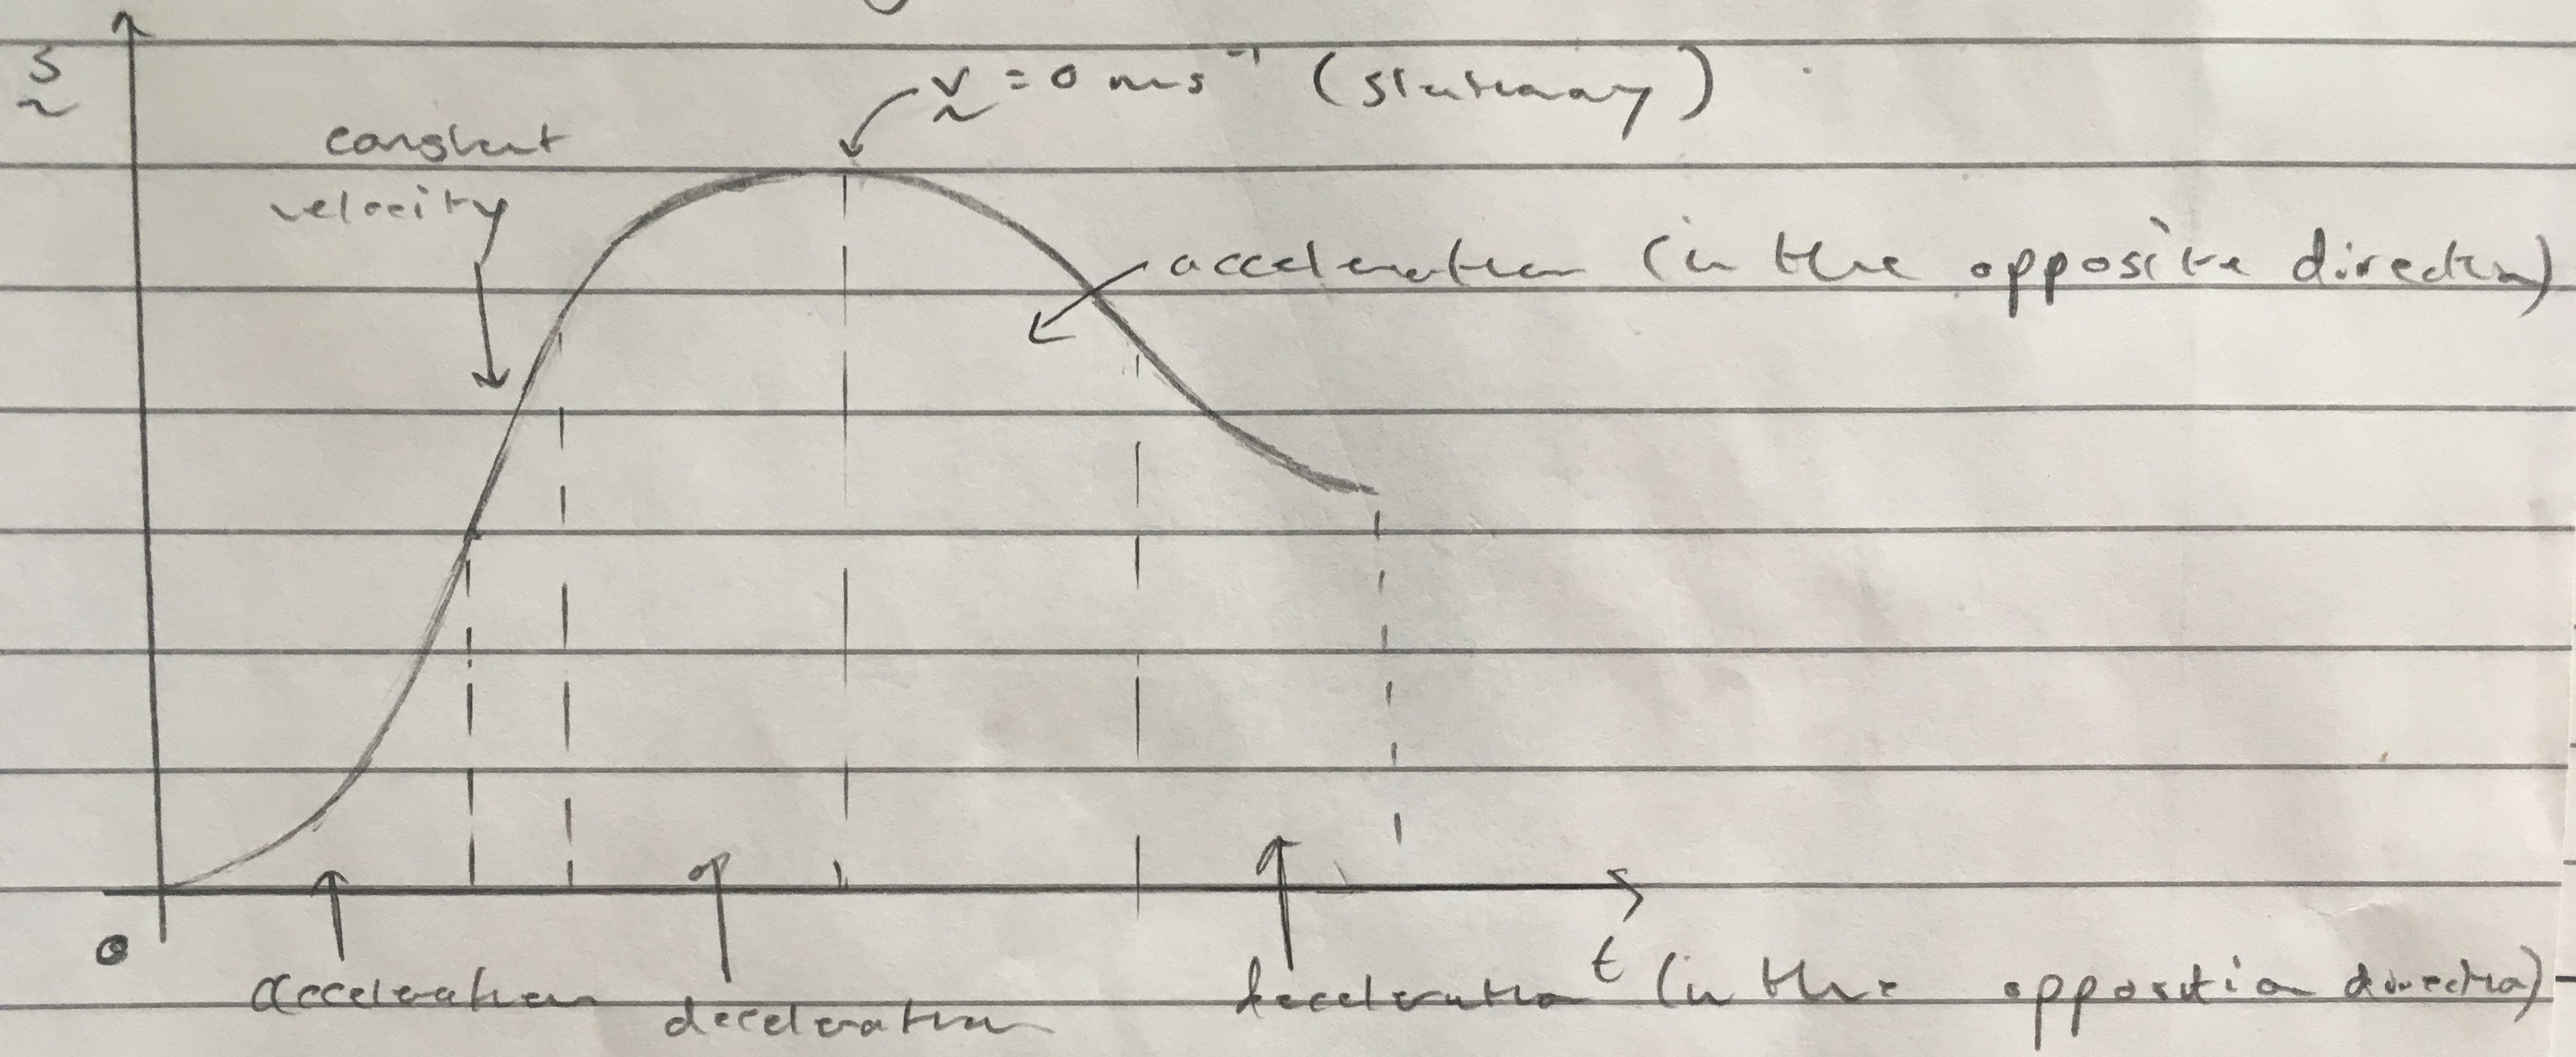
\includegraphics[scale=0.1]{notes/images/Displacement-Time-Graph.JPG}
    \caption{A \textit{s-t} graph}
\end{figure}
\FloatBarrier

\subsection{Distance and Speed}

The concept of velocity is associated with displacement, the concept of speed is associated with the distance travelled by the particle. Hence velocity is a vector quantity and speed is a scalar quantity. We note that due to the \textit{fundamental theorem of calculus} that 
\begin{equation*}
    \vec{s}(t) = \int \vec{v}(t) \mathop{\mathrm{d}t} 
\end{equation*}

\begin{definition}{(\textbf{Distance})}
\textit{The distance travelled $x(t)$, measured in metres ($m$),by the particle $p$ at time $t$ is given by }
\begin{equation}
    x(t) = \sum_{i = 1} ^ n \left|\int_{t_{i-1}}^{t_{i}} \vec{v}(t) \mathop{\mathrm{d}t}\right|
\end{equation}
\textit{where for all $i = 1, 2, \ldots, n$ we have $\vec{v}(t_i) = \vec{0}$ or $\vec{s}(t_i) = \vec{0}$ and $0 \leq t_1 < t_2 < \ldots < t_n \leq t$.}
\end{definition}
\noindent From our definition of distance, we can now define average speed. 
\begin{definition}{(\textbf{Average Speed})}
\textit{The average speed $\overline{v}(t)$, measured in metres per second ($ms^{-1}$), of a particle $p$ at time $t$ is given by}
\begin{equation}
    \overline{v}(t) = \frac{x(t)}{t}
\end{equation}
\end{definition}

\subsection{Distance-Time Graphs}

For a similar motivation to \textit{s-t} graphs, we often plot a distance against time graph, also known as \textit{displacement-time} (\textit{x-t}) graphs. We can use the graph to find the instantaneous speed, using a similar method for finding the instantaneous velocity and finding the distance travelled. To find the distance travelled we use the method of dissection to analyze sections of the journey. We then find the distance travelled in each section and sum up the distances from each section in the provided time ranges, to find the total distance travelled. 

\begin{figure}[h!]
    \centering
    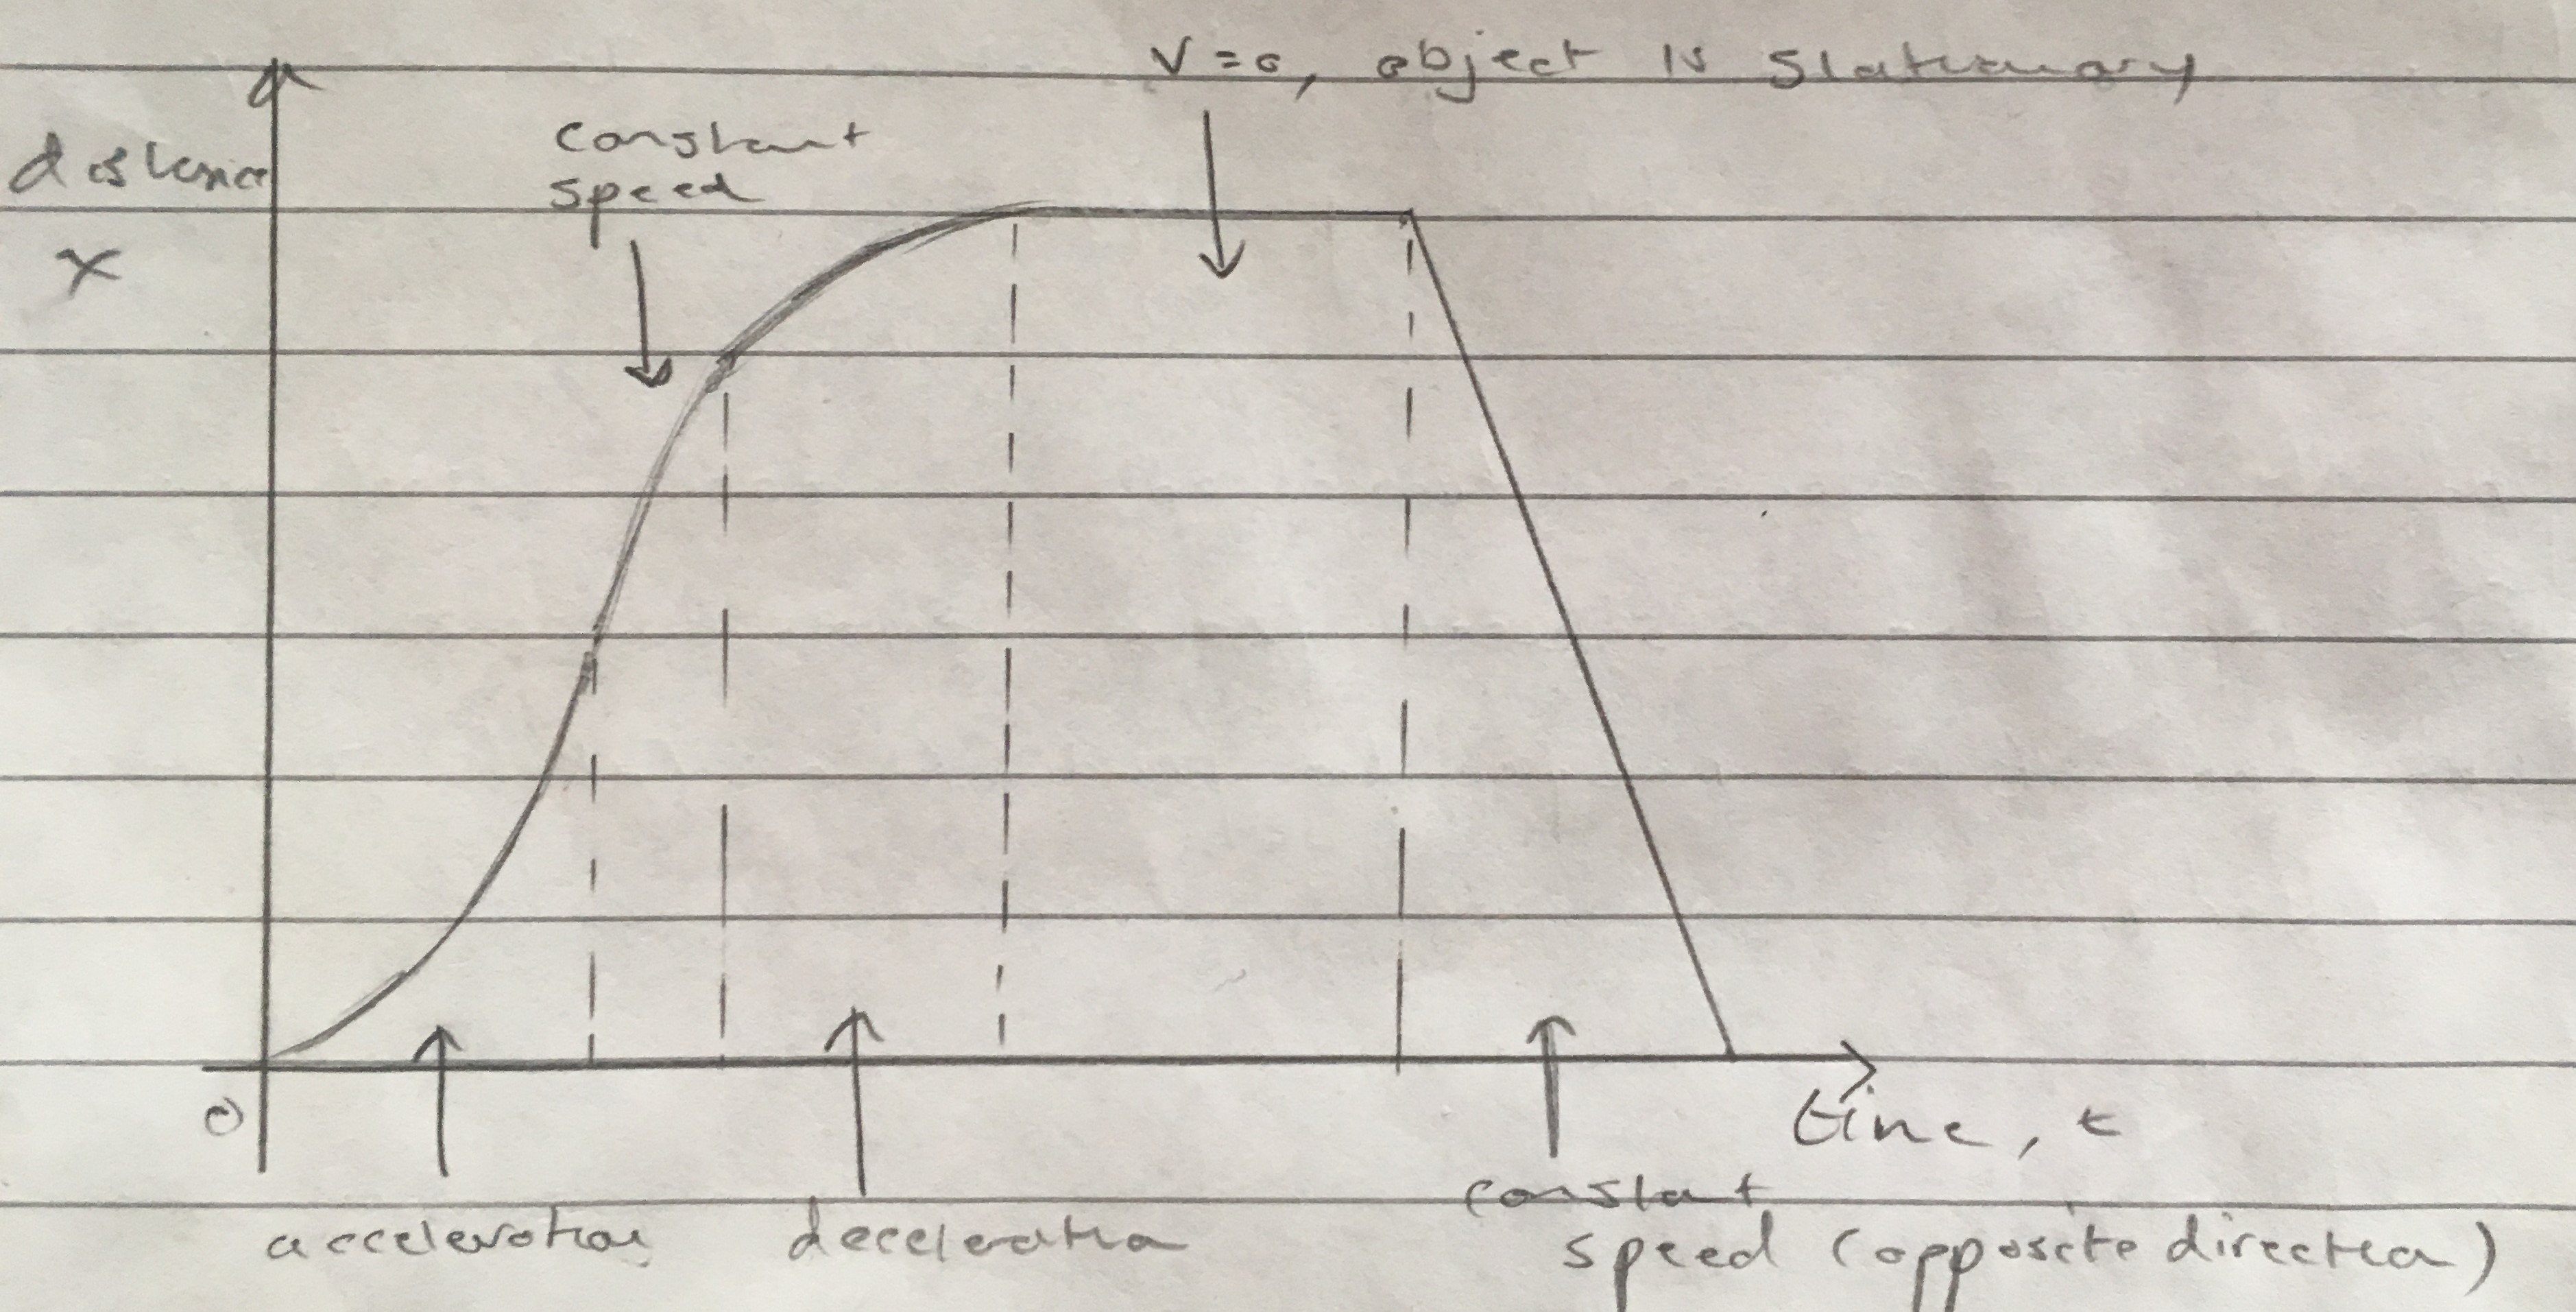
\includegraphics[scale=0.1]{notes/images/Distance-Time-Graph.jpg}
    \caption{A \textit{x-t} graph}
\end{figure}
\FloatBarrier

\subsection{Acceleration}

The last kinematic attribute of particle motion involves the determination of whether the instantaneous velocity $\vec{v}(t)$ of the particle changes as a function of time.

\begin{definition}{(\textbf{Acceleration})}
\label{def:acceleration}
\textit{The instantaneous acceleration $\vec{a}(t)$ of a particle $p$ is defined as the rate of change of the instantaneous velocity $\vec{v}(t)$: }
\begin{equation}
 \vec{a}(t) = \frac{\mathop{\mathrm{d}\vec{v}(t)}}{\mathop{\mathrm{d}t}}  
\end{equation}
\textit{measured in \textbf{metres per second squared} ($ms^{-2}$)}
\end{definition}
Note that the instantaneous acceleration of a particle can also be defined in terms of the section time derivative of its instantaneous displacement $\vec{s}(t)$.
\begin{equation*}
    \vec{a}(t) = \frac{\mathop{\mathrm{d}^2\vec{s}(t)}}{\mathop{\mathrm{d}t^2}}
\end{equation*}
Negative acceleration, or acceleration in the opposite direction to motion is usually called deceleration, however this might depend on the context of the scenario. 

\subsection{Velocity-Time Graphs}

For a similar motivation to \textit{s-t} and \textit{x-t} graphs, we often plot a velocity against time graph, also known as \textit{velocity-time} (\textit{v-t}) graphs. We can use the graph to find the instantaneous acceleration, using a similar method for finding the instantaneous velocity, and finding the displacement. To find the displacement using a \textit{v-t} graphs, we use the fundamental theorem of calculus, recalling that
\begin{equation*}
    \vec{s}(t) = \int \vec{v}(t) \mathop{\mathrm{d}t}.
\end{equation*}
Hence the area under a \textit{v-t} graph with bounds zero and $T$ seconds is equivalent to the displacement at time $T$. In A2 Physics we're not allowed to directly work with integrals, hence we must use the trapezium rule to estimate the area under the graph.  

\begin{figure}[h!]
    \centering
    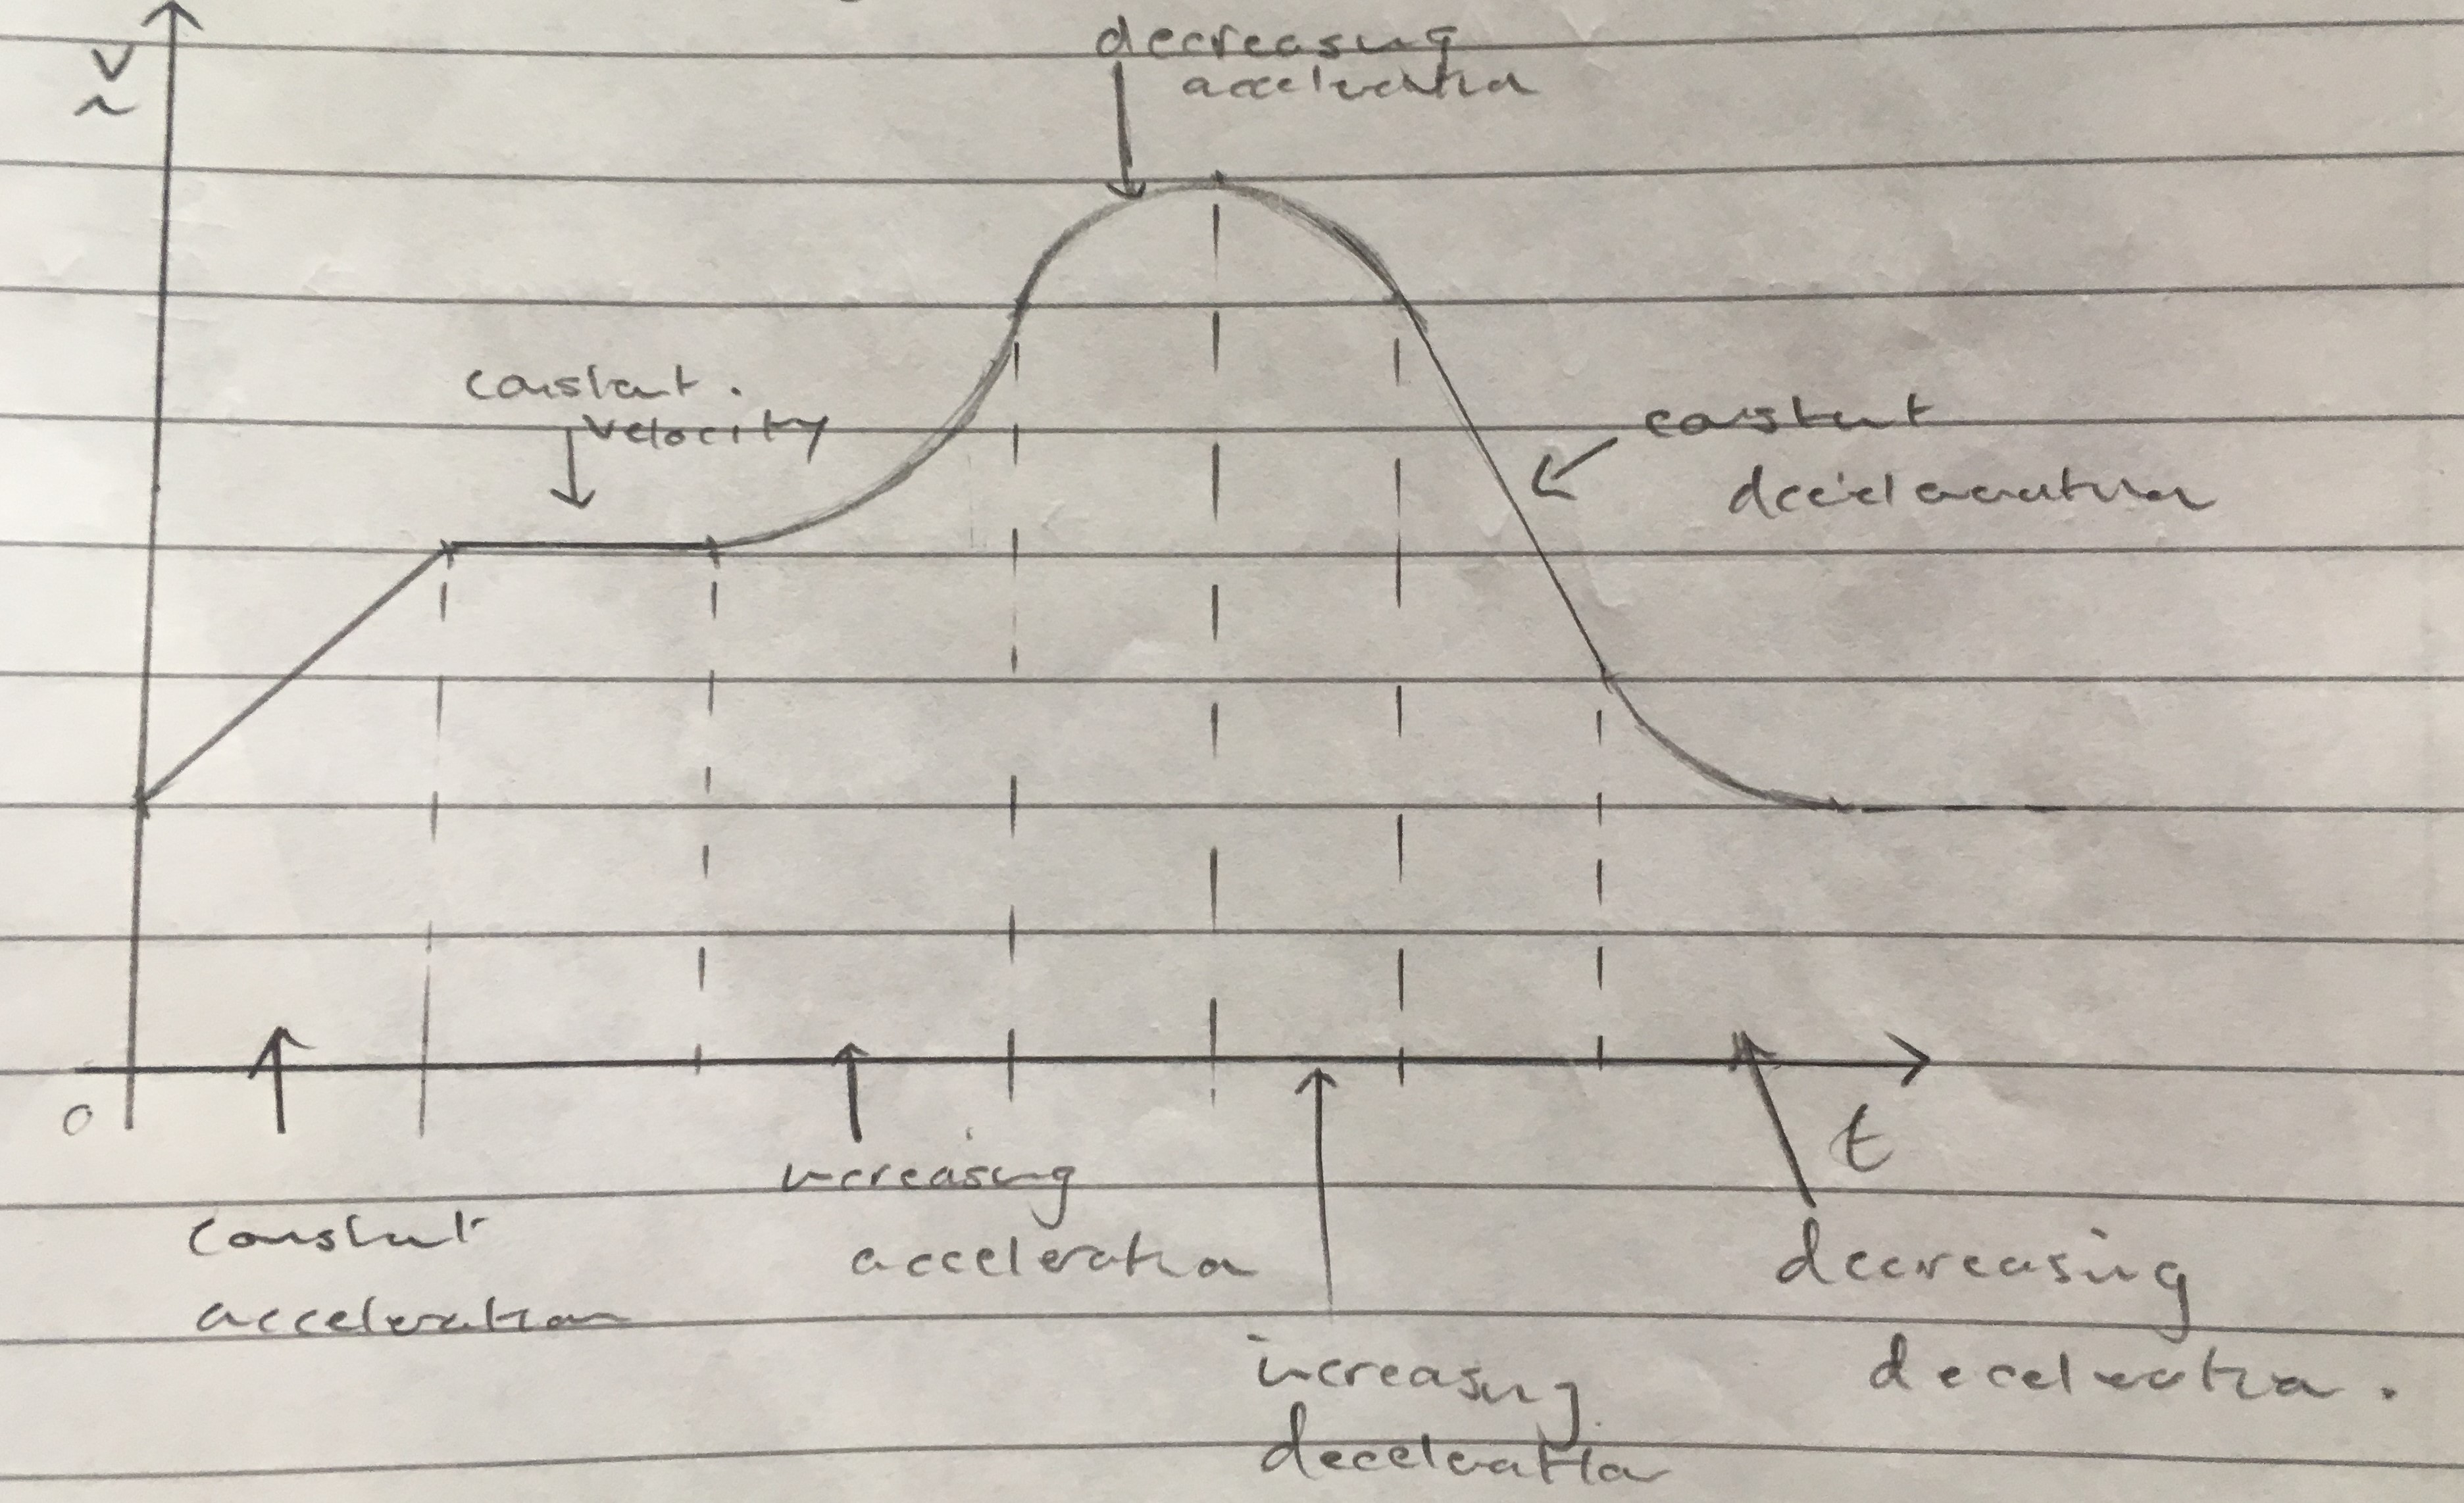
\includegraphics[scale=0.1]{notes/images/Velocity-Time-Graph.jpg}
    \caption{A \textit{v-t} graph}
\end{figure}
\FloatBarrier

\subsection{Equations of Motion}
\label{subsection:equations-of-motion}

This section will discuss one dimensional equations of motion for constant acceleration. It would be correct to say that no object has ever traveled in one-dimension with a constant acceleration anywhere in the universe at any time (due to relativity). However, it is useful to approximate real situations with models based on ideal situations (i.e constant acceleration). We will derive new equations that can be used to describe the motion of an object in terms of its three kinematic variables: acceleration $\vec{a}$, velocity $\vec{v}$, initial velocity $\vec{u}$, displacement $\vec{s}$ and time $t$. Since we are dealing with vector quantities, the use of vector calculus is necessary. 

By considering the definition of acceleration (see definition \ref{def:acceleration}), the fundamental theorem of calculus and assuming acceleration is constant, we get the velocity-time equation for constant acceleration, the so-called \textit{first equation of motion} (see equation \ref{eq:first-equation-of-motion}):
\begin{align*}
    \vec{a} &= \frac{\mathop{\mathrm{d}\vec{v}}}{\mathop{\mathrm{d}t}} \\
    \mathop{\mathrm{d}\vec{v}} &= \vec{a}\mathop{\mathrm{d}t} \\
    \int_{\vec{u}}^{\vec{v}} \mathop{\mathrm{d}\vec{v}} &= \int_0^t \vec{a}\mathop{\mathrm{d}t} \\
    \vec{v} - \vec{u} &= \vec{a}t,
\end{align*}
giving, 
\begin{equation}
    \label{eq:first-equation-of-motion}
    \vec{v} = \vec{u} + \vec{a}t.
\end{equation}

Again by definition, velocity is the first time derivative of displacement. Applying the fundamental theorem of calculus to this gives the displacement-time equation for constant acceleration, also known as the \textit{second equation of motion} (see equation \ref{eq:second-equation-of-motion})
\begin{align*}
    \vec{v} &= \frac{\mathop{\mathrm{d}\vec{s}}}{\mathop{\mathrm{d}t}} \\
    \mathop{\mathrm{d}\vec{s}} &= \vec{v}\mathop{\mathrm{d}t} \\
    \int_0^{\vec{s}} \mathop{\mathrm{d}\vec{s}} &= \int_0^t (\vec{u} + \vec{a}t) \mathop{\mathrm{d}t},
\end{align*}
evaluating the integral gives the second equation of motion,
\begin{equation}
    \label{eq:second-equation-of-motion}
    \vec{s}= \vec{u}t + \frac{1}{2}\vec{a}t^2.
\end{equation}

Unlike the first and second equations of motion, the \textit{third equation of motion} (see equation \ref{eq:third-equation-of-motion}), which relates velocity to displacement, cannot be obtained by reverse engineering the definitions of velocity or displacement. To do so, we need to consider the derivative of velocity with respect to displacement. 

\begin{equation*}
    \frac{\mathop{\mathrm{d}\vec{v}}}{\mathop{\mathrm{d}\vec{s}}} = \hspace{1mm} ?
\end{equation*}

To evaluate this derivative, we need to consider the chain rule. We note that the derivative above is equal to the product of acceleration and the inverse of velocity, that is
\begin{align*}
    \frac{\mathop{\mathrm{d}\vec{v}}}{\mathop{\mathrm{d}\vec{s}}} &= \frac{\mathop{\mathrm{d}\vec{v}}}{\mathop{\mathrm{d}t}} \cdot \frac{\mathop{\mathrm{d}t}}{\mathop{\mathrm{d}\vec{s}}} \\
    &= \vec{a} \cdot \frac{1}{\vec{v}}
\end{align*}

We should note that the reciprocal of a vector is mathematically speaking impossible, instead (in linear algebra) we consider the associated \textit{reciprocal vector} of $\vec{a}$, denoted $\vec{a}^{-1}$ such that $\vec{a} \cdot \vec{a}^{-1} = \vec{1}$. The next step is the separation of variables and then to integrate them. 

\begin{align*}
    \frac{\mathop{\mathrm{d}\vec{v}}}{\mathop{\mathrm{d}\vec{s}}} &= \vec{a} \cdot \frac{1}{\vec{v}} \\
    \vec{v} \cdot \mathop{\mathrm{d}\vec{v}} &= \vec{a} \cdot \mathop{\mathrm{d}\vec{s}} \\
    \int_{\vec{u}}^{\vec{v}} \vec{v} \cdot \mathop{\mathrm{d}\vec{v}} &= \int_0^{\vec{s}} \vec{a} \cdot \mathop{\mathrm{d}\vec{s}} \\
    \frac{1}{2}(\vec{v}\cdot \vec{v} - \vec{u} \cdot \vec{u}) &= \vec{a} \cdot \vec{s}
\end{align*}
The definition of the euclidean length of a vector $\vec{a}$, denoted $\| \vec{a} \|$, using dot product is $\| \vec{a} \| = \sqrt{\vec{a} \cdot \vec{a}}$, so we have 
\begin{equation}
    \label{eq:third-equation-of-motion}
    \| \vec{v} \|^2 = \| \vec{u} \|^2 + 2 \vec{a} \cdot \vec{s}.
\end{equation}
Alternatively, we could consider a one-dimensional model for each dimension in our model. For example, assuming that the motion takes places in two dimensions, we have
\begin{align*}
    v_x^2 &= u_x^2 + 2 a_x s_x, \\
    v_y^2 &= u_y^2 + 2 a_y s_y.
\end{align*}

We can now combine the three equations of motion to produce our so-called \textit{SUVAT} equations (shown below) where ``SUVAT'' is an acronym for the variables $\vec{s}$, $\vec{u}$, $\vec{v}$, $\vec{a}$ and $t$.
\begin{align}
    \vec{v} &= \vec{u} + \vec{a}t, \\
    \vec{s} &= \frac{1}{2}(\vec{u} + \vec{v})t, \\
    \vec{s} &= \vec{u}t + \frac{1}{2}\vec{a}t^2, \\
    \vec{s} &= \vec{v}t - \frac{1}{2}\vec{a}t^2, \\
    \| \vec{v} \|^2 &= \| \vec{u} \|^2 + 2\vec{a}\cdot \vec{s}.
\end{align}


\subsection{Free fall}

In physics, ``free fall'' is any motion of a body where gravity is the only force acting upon it. However the term is often used more loosely than the strict sense defined above. Thus, falling through an atmosphere without a deployed parachute is often referred to as \textit{free fall}. 

Newton's law of gravitation states that every body with mass attracts every other body in the universe  (see section ??). On earth, objects accelerate vertically downwards towards the centre of the earth due to this law. When an object is accelerating under ``gravity'', it is said to be in free fall (see above). The magnitude of the acceleration due to gravity, denoted by the symbol $\| \vec{g} \|$, is approximately $9.8$ $ms^{-2}$ on earth.   

In A2 Physics, we are required to know methods for determining this value. We will consider two experiments, the electromagnet and trap door method and the light gates method. 

\subsubsection{Electromagnet and Trap door}

An electromagnet holds a steel ball. When the current to the electromagnet is switch off, a timer is triggered as the magnet demagnetizes. When the magnet demagnetizes the ball is dropped. When the ball hits the trap door, the electrical contact is broken and the time stops. Applying the second equation of motion (under constant acceleration) we have  
\begin{equation}
    \vec{s} = \frac{1}{2}\vec{g}t^2.
\end{equation}
We can measure the displacement between the electromagnet and the trap door, so the only unknown left is the acceleration due to gravity $\vec{g}$. Rearranging the equation above, we can solve for $\vec{g}$.
\begin{equation}
    \vec{g} = \frac{2}{t^2}\vec{s}
\end{equation}
So we can just compute the magnitude of $\vec{g}$ to find an approximation to $\| \vec{g} \|$. The apparatus for this experiment is shown below. 

\subsubsection{Light Gates}

In theory, this method should be more accurate than the one described above, since light gates reduce the time delay. Place one light gate above another (vertically) with a known displacement $\vec{s}$ between them. Both light gates are then connected to a timer or data logger. A ball is dropped from through the first light gate triggering the timer to start. When the ball finally passes through the second light gate the timer stops. We can apply the same equation of motion we used in the method above to then find an approximate value of $\| \vec{g} \|$.


\subsection{Projectiles}

A projectile is any object that is cast, fired, flung, heaved, hurled or thrown. (This is an informal definition). The path of a project is called its \textit{trajectory}. Some examples of projects might include bullets, balls, rockets (after engine cut off), etc.

\begin{definition}{(\textbf{Projectile})}
\textit{A projectile is any object that once projected continues in motion by its own inertia and is influenced by the downwards force of gravity.}
\end{definition}

That is not to say other forces do not exist, just that they are negligible or have minimal effect in comparison. Another essential characteristics of a projectile is that its future has already been determined. Some projectiles travel far enough to experience a variation in acceleration due to gravity, for example a rocket will experience a variation in $\| \vec{g} \|$ by approximately $\pm 0.05$ $ms^{-2}$. To distinguish between projectiles that experience this variation, we use the term \textit{simple projectile}. For the remaining problems, the term \textit{general projectile} is adopted. 

Every projectile problem is essentially two one-dimensional motion problems, considering motion in the $x$ and $y$ planes. The kinematic equations for a simple projectile are those of an object traveling with constant horizontal velocity and a constant vertical acceleration, hence the equations of motion discussed in section \ref{subsection:equations-of-motion} can be applied. 

The equations of motion for a simple projectile are as follows
\begin{align}
    \vec{a}_x &= 0 & \vec{a}_y &= \vec{g} \\
    \vec{v}_x &= \vec{u}_x & \vec{v}_y &= \vec{u}_y + \vec{g}t \\
    \vec{s}_x &= \vec{u}_x t & \vec{s}_y &= \vec{u}_y t + \frac{1}{2} \vec{g}t^2 \\
    \hspace{1mm} & \hspace{1mm} & \| \vec{v}_y \|^2 &= \| \vec{u}_y \|^2 + 2 \vec{g} \cdot \vec{s} 
\end{align}
Note that any vectors in the above equations only exists in $\mathbb{R}$ and $\vec{g} = - \| \vec{g} \|$. Having obtained the equations of motion for a simple projectile, we can consider the maximum range of a projectile based on it's initial angle with the horizontal (note that this case only works with a projectile that has an initial horizontal and vertical position of zero). Considering the horizontal position, we have
\begin{align*}
    \vec{r}_x &= \vec{r}_{0, x} + \vec{u}_x t + \frac{1}{2} \vec{a}_x t^2 \\
    &= 0 + (\| \vec{u} \| \cos \theta) t + 0 \\
    &= (\| \vec{u} \| \cos \theta) t,
\end{align*}
so the final horizontal position is given by, 
\begin{equation*}
    \vec{r}_{x, final} = (\| \vec{u} \| \cos \theta) t_{final}.
\end{equation*}
Considering the vertical position, we have
\begin{align*}
    \vec{r}_y &= \vec{r}_{0, y} + \vec{u}_y t + \frac{1}{2} \vec{a}_y t^2 \\
    &= (\| \vec{u} \| \sin \theta) t - \frac{1}{2} \| \vec{g} \| t^2,
\end{align*}
and if we consider when $\vec{r}_y = 0$ (the final vertical position), we have
\begin{align*}
    0 &= (\| \vec{u} \| \sin \theta) t - \frac{1}{2} \| \vec{g} \| t_{final}^2 \\
    t_{final} &= \frac{2(\| \vec{u} \| \sin \theta)}{\| \vec{g} \|}.
\end{align*}
Combining these two equations,
\begin{align}
    \vec{r}_{x, final} &= (\| \vec{u} \| \cos \theta) \frac{2(\| \vec{u} \| \sin \theta)}{\| \vec{g} \|} \\
    &= \frac{\| \vec{u} \|^2 \sin 2\theta}{\| \vec{g} \|}.
\end{align}
If we consider the maximum of $\sin 2\theta$, then we get $\theta = \frac{\pi}{4}$. Hence the maximum range of a projectile with $\vec{r}_0 = \vec{0}$, denoted $\vec{r}_{x, max}$, is 
\begin{equation}
    \vec{r}_{x, max} = \frac{\| \vec{u} \|^2}{\| \vec{g} \|}.
\end{equation}

\subsection{Frames of reference}

A frame of reference is defined by a set of \textbf{coordinate axes} $(x, y, z)$ at rest relative to a particular observer. The observer can express the \textbf{position}, \textbf{velocity} and \textbf{acceleration} of a particle \textbf{relative to this frame of reference}. We want to consider transformations of these quantities between different frames of reference. This is particularly important in the \textbf{theory of relativity} (in modern physics). 

So for example, let us consider one frame of reference $S$, fixed relative to the Earth and another frame of reference $S'$ fixed relative to a car moving with a constant velocity $\vec{v}$ relative to the Earth, as shown in figure ??. 


Suppose the origins $O$ and $O'$ coincide at time $t = 0$. A point $P$ has the position $\vec{r}$ at time $t$ in $S$ and $\vec{r}'$ in $S'$, so that
\begin{equation*}
    \vec{r}' = \vec{r} - \vec{v}t 
\end{equation*}
Now suppose that point $P$ is moving at a constant velocity $\vec{u}$ relative to the Earth, then by definition
\begin{equation*}
    \vec{u} = \frac{\mathop{\mathrm{d}\vec{r}}}{\mathop{\mathrm{d}t}},
\end{equation*}
so the velocity of the point $P$ relative to the car is 
\begin{equation*}
    \vec{u}' = \frac{\mathop{\mathrm{d}\vec{r}'}}{\mathop{\mathrm{d}t}} = \frac{\mathop{\mathrm{d}\vec{r}}}{\mathop{\mathrm{d}t}} - \vec{v} = \vec{u} - \vec{v}
\end{equation*}

%So generally, if we consider a frame of reference $S$, relative to the Earth with a velocity $\vec{u}$ and another frame of reference $S'$, relative to the Earth with a velocity $\vec{v}$ and assuming the origins $O$ and $O'$ coincide at time $t = 0$ and the point $P$ has the position $\vec{r}_0$ at time $t=0$, then it has the position $\vec{r}$ in $S$ at time $t$ and $\vec{r}'$ in $S'$, so that
%\begin{align*}
%    \vec{r} &= \vec{r}_0 - \int_0^t \vec{u} \mathop{\mathrm{d}t} \\
%    \vec{r}' &= \vec{r} - \int_0^t \vec{v} \mathop{\mathrm{d}t} \\
%    &= \vec{r}_0 - \int_0^t \vec{u} + \vec{v} \mathop{\mathrm{d}t}
%\end{align*}
    
Now as we mentioned earlier, transformations of quantities is one of the key considerations in reference frames. So lets consider the transformation of velocity and acceleration. So the velocity of the point $P$ is  (from the example above)
\begin{equation*}
    \vec{u}' = \vec{u} - \vec{v}.
\end{equation*}
Suppose the velocity of the car $\vec{v}$ is constant, but the point $P$ is accelerating relative to the Earth, then
\begin{equation*}
    \frac{\mathop{\mathrm{d}\vec{u}'}}{\mathop{\mathrm{d}t}} = \frac{\mathop{\mathrm{d}\vec{u}}}{\mathop{\mathrm{d}t}} 
\end{equation*}
and the \textbf{acceleration} of the point is the \textbf{same} in both frames of reference. Suppose now that the car is also accelerating relative to the Earth, then 
\begin{equation*}
    \frac{\mathop{\mathrm{d}\vec{u}'}}{\mathop{\mathrm{d}t}} = \frac{\mathop{\mathrm{d}\vec{u}}}{\mathop{\mathrm{d}t}} - \frac{\mathop{\mathrm{d}\vec{v}}}{\mathop{\mathrm{d}t}} ,
\end{equation*}
with $\frac{\mathop{\mathrm{d}\vec{u}'}}{\mathop{\mathrm{d}t}}$ being the acceleration of the point relative to the car, $\frac{\mathop{\mathrm{d}\vec{u}}}{\mathop{\mathrm{d}t}}$ being the acceleration of the point relative to the Earth and  $\frac{\mathop{\mathrm{d}\vec{v}}}{\mathop{\mathrm{d}t}}$ being the acceleration of the car relative to the Earth. The force on the point necessary to accelerate in the frame $S$ is
\begin{equation*}
    \vec{F} = m \frac{\mathop{\mathrm{d}\vec{u}}}{\mathop{\mathrm{d}t}}.
\end{equation*}
The equation of motion of the point in the reference frame of the car, $S'$,
\begin{equation*}
    \vec{F}' = m \frac{\mathop{\mathrm{d}\vec{u}'}}{\mathop{\mathrm{d}t}} = m \frac{\mathop{\mathrm{d}\vec{u}}}{\mathop{\mathrm{d}t}} - m \frac{\mathop{\mathrm{d}\vec{v}}}{\mathop{\mathrm{d}t}} = \vec{F} - m \vec{a},
\end{equation*}
where $m$ is the mass of the point and $\vec{a} = \frac{\mathop{\mathrm{d}\vec{v}}}{\mathop{\mathrm{d}t}}$ is the acceleration of the car in frame $S$. Thus if we want to apply Newton's laws of motion in an accelerating frame, we must add to the \textbf{real} force $\vec{F}$ the \textbf{fictitious} force $-m\vec{a}$. An accelerating frame of reference is also called a \textbf{non-inertial} frame. An \textbf{inertial} frame of reference is one in which Newton's laws of motion apply \textbf{without} needing to introduce fictitious forces.

TODO: Generalize the relative positions, velocities and forces between two frames of reference with variable velocities and a point with a variable velocity

\section{Dynamics I : Forces}

In the first chapter, we discussed kinematics - the mathematical description of (ideal) motion. With the exception of a small number of topics, we never discussed the factors that affected motion. We will now study the quantities that affect motion - mass and force. The mathematical description of motion that includes these quantities is called \textit{dynamics}.

\subsection{Forces}
\label{subsection:forces}


Many intuitive approaches to Physics define a force as ``a push or a pull''. This is a reasonable informal definition to help us conceptualize a force, but it is a terrible definition. So what is a force?

\begin{itemize}
    \item A force is an interaction that will change the motion of any particle (if unopposed), or more generally, a force is an interaction that causes a change.
    \item Force is a vector quantity associated with an interaction.
    \item When several forces act on a system, it is the net force that matters. Since force is a vector quantity, we can use vector addition to compute the so-called \textit{resultant} force, written as $\vec{F}$.
\end{itemize}
Here are some examples of the forces we will discuss in this course:
\begin{itemize}
    \item Forces that act on all objects.
    \begin{itemize}
        \item Weight ($\vec{W}$, $\vec{F}_g$) \\
        The force of gravity acting on an object due to its mass. An object's weight is directed down, towards the center of the gravitating body
    \end{itemize}
    \item Forces associated with solids.
    \begin{itemize}
        \item Normal Contact Force ($\vec{N}$, $\vec{R}$, $\vec{F}_n$) \\
        The force between two objects in contact. The force prevents them from occupying the same space. The normal force is perpendicular to the surface of the object. 
        \item Friction ($\vec{F}_f$) \\
        The force between solids in contact that resists their sliding across one another. Friction is directed opposite to the direction of motion (or the intended direction of motion).
        \item Tension ($\vec{T}$, $\vec{F}_t$) \\
        The force exerted by an object that is being pulled upon from opposite ends. Examples of common objects that exert tension are string, rope, cables, etc. 
    \end{itemize}
    \item Forces associated with fluids. Fluids include liquids and gases.
    \begin{itemize}
        \item Buoyancy ($\vec{B}$, $\vec{F}_b$) \\
        The force exerted on an object immersed in a fluid. Buoyancy is sometimes referred to as upthrust.
        \item Drag ($\vec{D}$, $\vec{F}_d$) \\
        The force that resists the motion of an object through a fluid Drag is directed opposite to the direction of motion of the object relative to the fluid.
    \end{itemize}
\end{itemize}

There are other forces, such as electrostatic forces, magnetic forces and nuclear forces. However, we will not discuss those in this chapter. Having grasped the concept of force, we can now move onto Newton's laws of motion which laid the foundation for classical mechanics. 

\begin{theorem}{(\textbf{Newton's First Law of Motion})}
\textit{Newton's first law of motion states than an object either remains at rest or continues to move at a constant velocity, unless acted upon by a resultant force.}
\end{theorem}

\noindent The first law can be stated mathematically when the mass is a non-zero constant, as
\begin{equation}
    \vec{F} = \vec{0} \iff \frac{\mathop{\mathrm{d}\vec{v}}}{\mathop{\mathrm{d}t}} = \vec{0}.
\end{equation}
Consequently,
\begin{itemize}
    \item An object that is at rest will stay at rest unless a resultant force acts upon it.
    \item An object that is in motion will not change it's velocity unless a resultant force acts upon it. This is known as \textit{uniform motion}.
\end{itemize}
We could infer from the first law that motion is just as natural a state as is rest. 

\begin{theorem}{(\textbf{Newton's Second Law of Motion})}
\textit{The second law states that the rate of change of momentum (see section \ref{subsection:impulse-and-momentum}) of an object is directly proportional to the resultant force, and this change in momentum takes place in the direction of the resultant force.}
\begin{equation}
    \label{eq:second-law-of-motion}
    \vec{F} = \frac{\mathop{\mathrm{d}\vec{p}}}{\mathop{\mathrm{d}t}}.
\end{equation}
\begin{proof}
\textit{This proof refers to equation \ref{eq:second-law-of-motion}. From the second law, we have}
\begin{equation*}
    \vec{F} \propto \frac{\mathop{\mathrm{d}\vec{p}}}{\mathop{\mathrm{d}t}},
\end{equation*}
\textit{where $\vec{F}$ is the resultant force acting on the object. The relationship above can be written with a constant of proportionality $k$.}
\begin{equation*}
    \vec{F} = k \frac{\mathop{\mathrm{d}\vec{p}}}{\mathop{\mathrm{d}t}}.
\end{equation*}
\textit{We can say $k = 1$, by defining the unit of force, the \textbf{newton}, as the force required to give a unit mass an acceleration of $1$ $ms^{-2}$. Allowing Newton's second law of motion to be written mathematically as} 
\begin{equation*}
    \vec{F} = \frac{\mathop{\mathrm{d}\vec{p}}}{\mathop{\mathrm{d}t}}.
\end{equation*}
\end{proof}
\end{theorem}

\begin{definition}{(\textbf{The Newton})}
\textit{A newton is the force required to give a mass of $1$ kg an acceleration of $1$ $ms^{-2}$, thus}
\begin{equation*}
    [N] = [kgms^{-2}].
\end{equation*}
\end{definition}

If a body is at equilibrium (a state where the resultant force is zero), then it follows that Newton's first law is a direct result of the second law. In contrast, if we consider a constant-mass system with unbalanced forces acting upon a body, it will result in the body's momentum changing over time. Since the mass $m$ can be factored outside the differentiation operation by the linearity of the derivative, we have

\begin{align}
    \vec{F} &= \frac{\mathop{\mathrm{d}\vec{p}}}{\mathop{\mathrm{d}t}} \\
    &= \frac{\mathop{\mathrm{d}}}{\mathop{\mathrm{d}t}}(m \vec{v}) \\
    &= m \frac{\mathop{\mathrm{d}\vec{v}}}{\mathop{\mathrm{d}t}} \\
    &= m \vec{a},
\end{align}
where $\vec{F}$ is the resultant force, $m$ is the mass of the body and $\vec{a}$ is the body's acceleration. However, we should note that Newton's second law is valid only for constant-mass systems because of relativistic effects.

\begin{theorem}{(\textbf{Newton's Third Law of Motion})}
\textit{The third law, sometimes referred to the law of reaction, states the if object $B$ exerts a force $\vec{F}_{BA}$ on object $A$, then object $A$ exerts an equal and opposite reaction force of $\vec{F}_{AB}$ on object $B$, such that}
\begin{equation}
    \vec{F}_{AB} = -\vec{F}_{BA}.
\end{equation}
\end{theorem}

\subsection{Weight}

Weight is a force of gravity acting on an object. It follows from Newton's second law of motion that the weight of an object $\vec{W}$ is equal to the product of the mass of the object $m$ and the acceleration due to gravity $\vec{g}$. 
\begin{equation}
    \vec{W} = m\vec{g}.
\end{equation}

A common misconception is that weight and mass are equivalent (which is mainly due to english), although, we may have difficulty understanding mass since we have yet to formally define it. So what is mass? Mass is a scalar quantity associated with matter (more specifically, the amount of matter). The SI unit of mass is the \textbf{kilogram} $[kg]$. We note that this is an informal definition, but since mass is a fundamental quantity of mass, we cannot define it. 

\subsection{Centre of Mass}

\begin{definition}{(\textbf{Centre of Mass})}
\textit{The centre of mass is a point where the (entire) weight of the object (appears to) act.}
\end{definition} 

This definition is sufficient for our course, however, we are more inclined to a formal definition. So we say, the centre of mass is the unique point at the centre of a distribution of mass in space that has the property that the weighted position vectors relative to this point sum to zero. 

\subsubsection{A system of particles}

In the case of a system of particles $P$ with $n$ particles, where each particle $P_i$, $i = 1, 2, \ldots n$ is located in space with position $\vec{r}_i$ and mass $m_i$. The position of the centre of mass $\vec{R}$ must satisfy 
\begin{equation*}
    \sum_{i = 1}^n m_i (\vec{r}_i - \vec{R}) = \vec{0}.
\end{equation*}
Solving this equation for $\vec{R}$ yields
\begin{equation}
    \vec{R} = \frac{1}{M} \sum_{i=1}^n m_i \vec{r}_i,
\end{equation}
where $M$ is the sum of the masses of all of the particles in the system. 

\subsubsection{Locating the centre of mass}

We will consider two cases, bodies with an axis of symmetry and bodies without an axis of symmetry, of locating the centre of mass in two dimension. We note that by the \textit{pigeonhole principle} we're covering all possible two dimensional bodies.

\begin{itemize}
    \item \textit{Case 1}: Symmetrical Systems \\
    The centre of mass of a body with an invariant point along all symmetrical operations is it's centre of mass. This invariant point can be determined by considering the lines of symmetry (the symmetry operations, in group theory). The intersection of the lines of symmetry is the invariant point, and hence the centre of mass.
    \item \textit{Case 2}: Non-Symmetrical Systems \\
    An experimental method for locating the centre of mass is to suspend the object from two points and to drop \textbf{plumb} lines from the suspension points. The intersection of the two lines is the centre of mass. A plumb line is a line with a weight at the end, this ensures the plumb line is parallel to the gravity field.  
\end{itemize}

\subsection{Free Body Diagrams}

Physics is a simple subject taught by simpleminded folk. When physicists look at an object, their first instinct is to simplify that object (i.e make it a particle). 

Note that particle refers too a point mass, a theoretical point with mass assigned to it. A particle is usually used to model object whose other physical properties such as extent and volume do not influence the behavior of interest. 

To a physicist, a book isn't made up of pages of paper bound together with glue, it's a particle. A person doesn't have two arms, two legs and head; they're a particle. It is this mindset that allows us to produce a type of drawing used by physicists called a \textit{free body diagram}.

A free body diagram isolates all the forces acting on a particle. It is this process of logical analysis that allows us to break down complex situations into a set of simpler ones. 

\subsubsection{A book lying on a table}

Let us consider the age old example, a book lying on a table. (\textit{How exciting! Could there be anything more grand?}). Draw a box to represent the book (we could draw a circle or a point, but that would be silly). Draw a horizontal line under the box to represent the table. Now identify the forces acting on it. 

Since the book has a mass, we know the force of gravity is acting upon it. Gravity pulls the book down, but it doesn't fall down. So there must be some force that pushes the book up. The force that pushes the book up is known as the normal contact force (see section \ref{subsection:forces}). 

Are we done? In terms of identifying the forces, yes we are. We can now begin to draw our free body diagram, but a problem quickly arises. How long should we draw the arrows representing each force. Since the book is at rest, it follows from Newton's first law of motion, the resultant force is zero. So we have
\begin{equation*}
    \vec{F} = \vec{R} + \vec{W} = \vec{0}.
\end{equation*}
Hence the forces are of equal magnitude. In summary, draw a box with two arrows of equal lengths coming out of the centre, one pointing up and one pointing down, label the one pointing down weight and the one pointing up normal; as shown in figure \ref{fig:free-body-diagram-book}. 

\begin{figure}[h!]
    \centering
    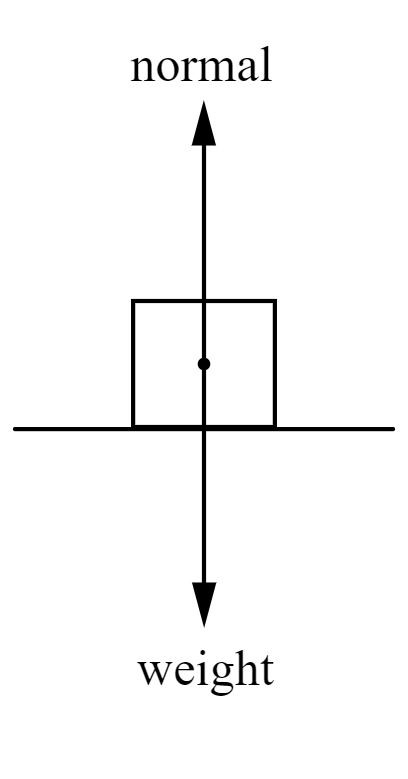
\includegraphics[scale=0.75]{notes/images/Free-Body-Diagram-Book.JPG}
    \caption{A free body diagram of a book lying on a table}
    \label{fig:free-body-diagram-book}
\end{figure}
\FloatBarrier

\subsection{Statics}

Informally, statics is the study of forces without motion. More formally, statics is the branch of mechanics that deals with forces in the absence of changes in motion. In contrast, dynamics is the study of forces and motion; or more formally, the branch of mechanics that deals with the effect that forces have on the motion of bodies. Statics implies stasis. Dynamics implies change (acceleration). 

Statics seems to imply being stationary, but it is not the case; it is merely the absence of acceleration that distinguishes statics from dynamics. When an object doesn't accelerate, it has no resultant force acting on it. This is a consequence of Newton's first law of motion. There are several ways of describing such a situation:
\begin{itemize}
    \item The resultant force is zero.
    \item The forces are balanced.
    \item The system is in equilibrium.
\end{itemize}
The ``resultant force is zero'' relates back to the first law. The resultant force, sometimes referred to as the \textit{net force}, relates to the vector sum of all the separate forces acting on the object. This can be written as $\sum \vec{F}$ or $\vec{F}$. So in a ``statics'' situation $\vec{F} = \vec{0}$.

The ``forces are balanced'' is usually used in situations such as a book on a table, the weight is balanced by the normal contact force from the table. Weight and normal in this case are said to be a pair of balanced forces because one is equal and opposite to the other (note that this is a action-reaction pair of forces in this scenario). If we have a pair of balanced forces, their vector sum is zero. If all the forces on an object are balanced, then we can safely say the forces acting on an object are balanced if and only if the resultant force is zero. Hence providing the equivalence between to first and second statements. We will not discuss the third statement, as we have already mentioned it in passing in other sections (see section \ref{subsection:forces}).  


\subsection{Friction}

As stated in section \ref{subsection:forces}. Friction refers to any force that resists relative tangential motion (or intended motion), whose direction is opposite to the relative direction of motion (or intended motion). ``Relative tangential motion'' is a fancy way to say slipping or sliding. 

There are several types of friction. Although we will only discuss dry and viscous friction in this course. Dry friction ($\vec{F}_f$) is the resistive force between solid surfaces in contact that resist their relative tangential motion, whereas, viscous friction is the resistive force between surfaces in relative motion through a fluid. For example, drag is a type of viscous friction. Viscous friction is dealt with in a different section, see \ref{subsection:drag}. There are a number of factors affecting dry friction:
\begin{itemize}
    \item The magnitude of dry friction $\| \vec{F}_f \|$ is directly proportional to the magnitude of normal contact force $\| \vec{R} \|$ between the two surfaces in contact.
    \item The magnitude of dry friction $\| \vec{F}_f \|$ depends on the materials in contact. This factor is measured by the quantity known as the \textit{coefficient of friction} $\mu$ which exists in the range $0 \leq \mu \leq 1$. Hence the magnitude of dry friction is directly proportional to the coefficient of friction.
\end{itemize}

\noindent We typically divide dry friction into two distinct types: static friction and kinetic friction. 

\begin{itemize}
    \item \textbf{Static friction} ($\vec{F}_{f, s}$) \\
    Static friction, also known as \textit{starting friction}, occurs when the two surfaces in contact \textit{are not} in relative motion; that is, when one surface is stationary relative to the other surface. The magnitude of static frictions varies from zero (when no external force is trying to force slippage) to some maximum value (just before slippage occurs). This maximum value can be determined using the inequality stated below.
    \begin{equation}
        \| \vec{F}_{f, s} \| \leq \mu_s \| \vec{R} \|,
    \end{equation}
    where $\mu_s$ denotes the coefficient of static friction.
    \item \textbf{Kinetic friction} ($\vec{F}_{f, k}$) \\
    Kinetic friction, also known as \textit{sliding} or \textit{dynamic} friction, occurs when two surfaces in contact \textit{are} in relative motion; that is when one surface is slipping or sliding across another surface. The magnitude of kinetic friction varies in a similar fashion to static friction and is always less than the maximum magnitude of static friction. So we have the following relationship;
    \begin{equation}
        \| \vec{F}_{f, k} \| = \mu_k \| \vec{R} \| < \mu_s \| \vec{R} \|,
    \end{equation}
    where $\mu_k$ denotes the coefficient of kinetic friction.
    
    
\end{itemize}


\section{Energy}

\subsection{Work}

If a force is applied to a body, which then moves, we say the force does \textbf{work}. In one-dimension, if the force is \textit{constant} with magnitude $F$, and the body moves a distance $x$, the work done $W$ is 
\begin{equation}
    W = Fx
\end{equation}

\begin{definition}{(\textbf{Work})}
\label{def:work}
\textit{The work done, W, is defined as the product of the magnitude of the force parallel to the direction of motion, $F_{\|}$, and the distance moved $x$ in the direction of motion}
\begin{equation}
    W = F_{\|} x
\end{equation}
\textit{measured in \textbf{joules} (J).}
\end{definition}

\begin{definition}{(\textbf{Joule})}
\textit{A joule is the work done by a force of 1 newton moving through a distance of 1 metre, thus }
\begin{equation*}
    [J] = [Nm] = [kgm^2s^{-2}]
\end{equation*}
\end{definition}

However, the definition of work done (see definition \ref{def:work}) only applies to a one-dimensional model and when the force is applied in the direction of motion. In two-dimensions, the force applied can be at an angle to the direction. The component of the force $\vec{F}$ that is parallel to the direction of motion is $\| \vec{F} \| \cos \theta$, where $\theta$ is the angle between the force and the direction of motion. So, in two-dimensions work done, $W$, is defined as
\begin{equation}
    W = \| \vec{F} \| x\cos \theta
\end{equation}

If we consider the individual dimensions of a multidimensional model and calculated the work done in all dimensions. Summing these produces the total work done. Hence we can consider the dot product of force and displacement to calculate the work done in a multidimensional model.

\begin{definition}{(\textbf{Work})}
\textit{The work done, W, is defined as the \textbf{dot product} of the constant force applied to an object $\vec{F}$ that moves a displacement $\vec{s}$}
\begin{equation}
    W = \vec{F} \cdot \vec{s} 
\end{equation}
\textit{measured in \textbf{joules} (J).}
\end{definition}

If the force is not \textit{constant}, then we must consider a small amount of work done $\mathop{\mathrm{d}W}$ with a force  $\vec{F}$ that moves an object a small displacement $\mathop{\mathrm{d}\vec{s}}$
\begin{equation*}
    \mathop{\mathrm{d}W} = \vec{F} \cdot \mathop{\mathrm{d}\vec{s}} = \vec{F} \cdot \vec{v} \mathop{\mathrm{d}t}
\end{equation*}
which forms a first order differential equation
\begin{equation*}
    \frac{\mathop{\mathrm{d}W}}{\mathop{\mathrm{d}t}} = \vec{F} \cdot \vec{v}
\end{equation*}
and can be solved using
\begin{equation}
    \label{eq:work-done-variable-force-vector}
    W = \int_{t_1}^{t_2} \vec{F} \cdot \vec{v} \mathop{\mathrm{d}t} = \int_{t_1}^{t_2} \vec{F} \cdot \frac{\mathop{\mathrm{d}\vec{s}}}{\mathop{\mathrm{d}t}} \mathop{\mathrm{d}t} = \int_C \vec{F} \cdot \mathop{\mathrm{d}\vec{s}}.
\end{equation}

\subsection{Power}
\label{subsection:power}

\begin{definition}{(\textbf{Power})}
\label{def:power}
\textit{Power, P, is defined as the rate of work done, so}
\begin{equation}
    P = \frac{\mathop{\mathrm{d}W}}{\mathop{\mathrm{d}t}}
\end{equation}
\textit{measured in \textbf{watts} (W)}
\end{definition}

\begin{corollary}
\textit{It follows, that if the force $\vec{F}$ is constant then power $P$ is}
\begin{equation}
    P = \vec{F} \cdot \vec{v}
\end{equation}
\textit{where $\vec{v}$ is velocity.}

\begin{proof}
\textit{By definition of power we have}
\begin{equation*}
    P = \frac{\mathop{\mathrm{d}W}}{\mathop{\mathrm{d}t}}
\end{equation*}
\textit{If the force $\vec{F}$ is constant, by definition we have}
\begin{equation*}
    \mathop{\mathrm{d}W} = \vec{F} \cdot \mathop{\mathrm{d}\vec{s}}
\end{equation*}
\textit{then,}
\begin{equation*}
    P = \vec{F} \cdot \frac{\mathop{\mathrm{d}\vec{s}}}{\mathop{\mathrm{d}t}} = \vec{F} \cdot \vec{v}.
\end{equation*}
\end{proof}
\end{corollary}

\subsection{Energy}
\label{subsection:energy}
If a body has the capacity (or ability) to do work, we say it has \textbf{energy}.
\begin{definition}{(\textbf{Energy})}
\textit{Energy is defined as the capacity for doing work, which implies, the energy of the body is amount of work it can do. Measured in \textbf{joules} (J).}
\end{definition}

When the body does some work it uses some of it's energy, but if work is done on the body then it's energy increases. Energy comes in many forms (thermal, electrical, \ldots) but we consider only \textit{mechanical energy} (in section \ref{subsection:energy}). Mechanical energy is of two types;
\begin{enumerate}
    \item \textit{kinetic energy} - the ability to do work by virtue of velocity.
    \item \textit{potential energy} - ability to do work by virtue of position in a gravitational field.
\end{enumerate}

\subsection{Equivalence of Work and Energy}

When work is done on a body by applying a force which moves through a distance, then it's energy increases by the amount of work done.
Similarly, a body which possesses energy, either kinetic or potential, can give up that energy by doing work. Hence we say \textbf{Work and Energy are equivalent} and are both measured in \textit{\textbf{Joules} (J)}.

\subsection{Conservation of Energy}

If no work is done on or by a body, then body is said to be in a \textbf{closed system}. We say:

\begin{center}
    \textit{The total energy of a closed system remains constant. The energy can never be created or destroyed, but it can be transferred from one from to another.}
\end{center}

\noindent This is called the \textbf{Principle of conservation of energy}.

\subsection{Kinetic Energy}

\begin{definition}{(\textbf{Kinetic Energy})}
\textit{The kinetic energy of a body, $E_k$, with a mass $m$ and velocity $v$ is given by}
\begin{equation}
    E_k = \frac{1}{2}m \| \vec{v} \|^2
\end{equation}
\textit{measured in \textbf{joules} (J).}
\begin{proof}
\textit{Consider a particle of mass $m$ that is accelerated from rest to velocity $\vec{v}$ in a distance $\| \vec{s} \|$ by a constant force $\vec{F}$. From the equation of motion $\| \vec{v} \|^2 = \| \vec{u} \|^2 + 2\vec{a} \cdot \vec{s}$ and Newton's II law of motion, we have}
\begin{equation*}
    \| \vec{v} \|^2 = \frac{2}{m} \vec{F} \cdot \vec{s}
\end{equation*}
\begin{equation*}
    \vec{F} \cdot \vec{s} = \frac{1}{2}m\| \vec{v} \|^2
\end{equation*}
\textit{The work done by the force is entirely transferred to the Kinetic energy of the particle. Therefore}
\begin{equation*}
    W = E_k = \vec{F} \cdot \vec{s}
\end{equation*}
\textit{Hence}
\begin{equation*}
    E_k = \frac{1}{2}m \| \vec{v} \|^2
\end{equation*}
\end{proof}
\end{definition}

\subsection{Potential Energy}

\textbf{Potential energy}, also referred to as \textbf{gravitational potential energy}, is the capacity for doing work as a result of an object's position in a gravitational field.

\begin{definition}{(\textbf{Potential Energy})}
\textit{The potential energy of a body, $E_p$, with mass $m$ and change in height $h$ in a \textbf{uniform gravitational field} with gravitational field strength $\| \vec{g} \|$ is}
\begin{equation}
    E_p = m\| \vec{g} \|h
\end{equation}
\end{definition}

\begin{corollary}
\textit{In many situations, potential energy and kinetic energy are exchanged. For example, when an object falls its $E_p$ decreases while its $E_k$ increases. It follows from the \textbf{principle of conservation of energy}, that the lost in $E_p$ is equal to the gain in $E_k$}
\begin{align*}
    m\| \vec{g} \|h &= \frac{1}{2}m\| \vec{v} \|^2 \\
    \| \vec{g} \|h &= \frac{1}{2} \| \vec{v} \|^2 \\
    \| \vec{v} \|^2 &= 2\| \vec{g} \|h \\
    \| \vec{v} \| &= \sqrt{2\| \vec{g} \|h}
\end{align*}
\textit{provided the system is closed and the change in height $h > 0$}.
\end{corollary}

\section{Dynamics II: Momentum}

\subsection{Impulse and Momentum}
\label{subsection:impulse-and-momentum}

Momentum keeps me going. It is a ``quantity of motion'' (from \textit{Principa}). Almost a resistance to stopping. 

\begin{definition}{(\textbf{Momentum})}
\textit{Momentum is the product of the mass and velocity of an object. Mathematically, }
\begin{equation}
    \vec{p} = m \vec{v},
\end{equation}
\textit{where $\vec{p}$ is the momentum of the object (a vector quantity), m is the object's mass and $\vec{v}$ is the velocity. It is measured in \textbf{kilogram meters per second} ($kgms^{-1}$)}
\end{definition}

We know from Newton's second law of motion, that the resultant force is directly proportional to the rate of change of momentum. 
\begin{equation*}
    \vec{F} = \frac{\mathop{\mathrm{d}\vec{p}}}{\mathop{\mathrm{d}t}}.
\end{equation*}
Separating the variables, we have
\begin{equation*}
    \vec{F} \mathop{\mathrm{d}t} = \mathop{\mathrm{d}\vec{p}},
\end{equation*}
integrating both sides yields a new quantity. We'll call it \textbf{impulse}, denoted by the letter $\vec{J}$. Thus,
\begin{equation}
    \label{eq:impulse-momentum-theorem}
    \vec{J} = \int_{\vec{p}_0}^{\vec{p}_1} \mathop{\mathrm{d}\vec{p}} = \int_0^t \vec{F} \mathop{\mathrm{d}t}
\end{equation}
Impulse is measured in \textit{newton seconds} or \textit{kilogram meters per second} which is dimensionally equivalent to momentum. This relationship is called the \textbf{impulse-momentum theorem}, which states that \textit{impulse causes a change in momentum}. Evaluating the first integral in equation \ref{eq:impulse-momentum-theorem} give us
\begin{equation}
    \vec{J} = \vec{p}_1 - \vec{p}_0 = \Delta \vec{p} = \int_0^t \vec{F} \mathop{\mathrm{d}t}.
\end{equation}

\subsection{Conservation of Momentum}

Suppose that two particles interact labelled one and two respectively. Because of the third law of motion, the forces between them are equal and opposite, so we have
\begin{equation}
    \vec{F}_{1,2} = - \vec{F}_{2,1}.
\end{equation}
The second law states that
\begin{equation}
    \vec{F}_{1,2} = \frac{\mathop{\mathrm{d}\vec{p}_1}}{\mathop{\mathrm{d}t}} \text{ and } \vec{F}_{2,1} = \frac{\mathop{\mathrm{d}\vec{p}_2}}{\mathop{\mathrm{d}t}}.
\end{equation}
Therefore,
\begin{equation}
    \frac{\mathop{\mathrm{d}}}{\mathop{\mathrm{d}t}} (\vec{p}_1 + \vec{p}_2) = \vec{0},
\end{equation}
implying that $\vec{p}_1 + \vec{p}_2$ is constant over time. So in a closed system the total momentum is constant. Hence we can say
\begin{align}
    \vec{p}_1 + \vec{p}_2 &= \vec{p}_1^{'} + \vec{p}_2^{'} \\
    \sum \vec{p} &= \sum \vec{p}'
\end{align}

\subsection{Collisions}

The conservation of momentum, discussed in the previous section, can be applied to collisions to determine the motion of particles after a collision. Another property of motion, kinetic energy, is also required to determine the motion of particles after collision. However, this is not necessarily conserved. If it is conserved, the collision is called an \textit{elastic} collision; if not, it is an \textit{inelastic collision}.  

If we consider an elastic collision between two particles, then by the conservation of momentum we have
\begin{equation}
    \vec{p}_1 + \vec{p}_2 = \vec{p}_1^{'} + \vec{p}_2^{'}.
\end{equation}
Let particle one have a mass of $m_1$ kg and an initial and final velocity of $\vec{u}_1$ and $\vec{v}_1$ respectively. Similarly for particle two, we apply the same labelling scheme. So from the definition of momentum, it follows that
\begin{equation}
    m_1 \vec{u}_1 + m_2 \vec{u}_2 = m_1 \vec{v}_1 + m_2 \vec{v}_2.
\end{equation}
If the both masses and three of the velocities are known, then it is possible to determine the unknown velocity.

\section{Rotational Motion}

\subsection{Motion in Plane Polar Coordinates}

A particle of mass $m$ may have a position $\vec{r}$ defined by a column vector, that is $\vec{r} = \langle r_1, r_2, \ldots, r_n \rangle$ or a \textbf{polar vector} with a magnitude $r$ and a direction $\theta$ such that $\vec{r} = \langle r, \theta \rangle$. Let us introduce a unit radial vector $\hat{r}$ and a unit transverse vector $\hat{\theta}$; where $\hat{r}$ and $\hat{\theta}$ are orthogonal (perpendicular) to each other. The position vector $\vec{r}$ is now given by $\vec{r} = r \hat{r}$. For example, in a two dimensional model the unit radial and transverse vectors are given by
\begin{align*}
    \hat{r} &= \langle \cos \theta, \sin \theta \rangle \\
    \hat{\theta} &= \langle - \sin \theta, \cos \theta \rangle
\end{align*}
As the particle moves in a two dimensional model, the magnitude $r$ and directions of $\hat{r}$ and $\hat{\theta}$ vary, implying they're functions of time. If we now consider the velocity of the particle, we find
\begin{equation}
    \vec{v} = \frac{\mathop{\mathrm{d} \vec{r}}}{\mathop{\mathrm{d} t}} = \frac{\mathop{\mathrm{d}}}{\mathop{\mathrm{d}t}}(r \hat{r}) = \frac{\mathop{\mathrm{d}r}}{\mathop{\mathrm{d} t}} \hat{r} + r \frac{\mathop{\mathrm{d} \hat{r}}}{\mathop{\mathrm{d} t}}
\end{equation}
An expression for $\frac{\mathop{\mathrm{d} \hat{r}}}{\mathop{\mathrm{d} t}}$ can be found by considering the expression for the unit radial vector (shown above), so we have
\begin{align*}
    \hat{r} &= \langle \cos \theta, \sin \theta \rangle \\
    \frac{\mathop{\mathrm{d} \hat{r}}}{\mathop{\mathrm{d} t}} &= \left\langle - \sin \theta \frac{\mathop{\mathrm{d} \theta}}{\mathop{\mathrm{d}t}}, \cos \theta \frac{\mathop{\mathrm{d} \theta}}{\mathop{\mathrm{d} t}}\right\rangle \\
    &= \frac{\mathop{\mathrm{d} \theta}}{\mathop{\mathrm{d}t}} \langle -\sin \theta, \cos \theta \rangle \\
    &= \frac{\mathop{\mathrm{d} \theta}}{\mathop{\mathrm{d}t}} \hat{\theta},
\end{align*}
So 
\begin{equation}
    \vec{v} = \frac{\mathop{\mathrm{d}r}}{\mathop{\mathrm{d} t}} \hat{r} + r \frac{\mathop{\mathrm{d} \theta}}{\mathop{\mathrm{d} t}} \hat{\theta}
\end{equation}
We say the radial component of $\vec{v}$ is $\frac{\mathop{\mathrm{d}r}}{\mathop{\mathrm{d} t}}$ and the transverse component is $r \frac{\mathop{\mathrm{d} \theta}}{\mathop{\mathrm{d} t}}$. An often used abbreviation for differentiation with respect to time is to put a ``dot'' above the quantity, so for the above expression for $\vec{v}$ is written as
\begin{equation}
    \vec{v} = \dot{\vec{r}} = \dot{r} \hat{r} + r \dot{\theta} \hat{\theta}
\end{equation}
The instantaneous speed of the particle  is given by
\begin{equation}
    \label{eq:polar-speed}
    v = \| \vec{v} \| = \sqrt{\vec{v} \cdot \vec{v}} = \sqrt{\left(\frac{\mathop{\mathrm{d}r}}{\mathop{\mathrm{d} t}}\right)^2 + r^2 \left(\frac{\mathop{\mathrm{d} \theta}}{\mathop{\mathrm{d} t}}\right)^2} = \sqrt{\dot{r}^2 + r^2 \dot{\theta}^2}.
\end{equation}
We now consider the acceleration of the particle, applying the product rule again to give
\begin{align*}
    \vec{a} &= \frac{\mathop{\mathrm{d}\vec{v}}}{\mathop{\mathrm{d}t}} = \frac{\mathrm{d}}{\mathop{\mathrm{dt}}} \left(\frac{\mathop{\mathrm{d}r}}{\mathop{\mathrm{d} t}} \hat{r} + r \frac{\mathop{\mathrm{d} \theta}}{\mathop{\mathrm{d} t}} \hat{\theta}\right) \\
    &= \frac{\mathop{\mathrm{d}^2 r}}{\mathop{\mathrm{dt^2}}} \hat{r} + \frac{\mathop{\mathrm{d}r}}{\mathop{\mathrm{d}t}} + 2 \frac{\mathop{\mathrm{d}r}}{\mathop{\mathrm{d}t}}\frac{\mathop{\mathrm{d}\theta}}{\mathop{\mathrm{d}t}} \hat{\theta} + r \hat{\theta} \frac{\mathop{\mathrm{d}^2 \theta}}{\mathop{\mathrm{d}t^2}} + r \frac{\mathop{\mathrm{d}\theta}}{\mathop{\mathrm{d}t}} \frac{\mathop{\mathrm{d}\hat{\theta}}}{\mathop{\mathrm{d}t}}
\end{align*}
Using the same method we used to find $\ddot{\hat{r}}$, we find that
\begin{equation*}
    \frac{\mathop{\mathrm{d} \hat{\theta}}}{\mathop{\mathrm{d} t}} = - \frac{\mathop{\mathrm{d} \theta}}{\mathop{\mathrm{d} t}} \hat{r},
\end{equation*}
so we have
\begin{align}
    \vec{a} &= \left(\frac{\mathop{\mathrm{d}^2 r}}{\mathop{\mathrm{d}t^2}} - r \left(\frac{\mathop{\mathrm{d}\theta}}{\mathop{\mathrm{d}t}}\right)^2 \right) \hat{r} + \left(2 \frac{\mathop{\mathrm{d}r}}{\mathop{\mathrm{d}t}} \frac{\mathop{\mathrm{d}\theta}}{\mathop{\mathrm{d}t}} + r \frac{\mathop{\mathrm{d}^2 \theta}}{\mathop{\mathrm{d}t^2}}\right) \hat{\theta} \\
    &= \left(\ddot{r} - r \dot{\theta}^2 \right) \hat{r} + \left(2 \dot{r} \dot{\theta} + r \ddot{\theta}\right) \hat{\theta}
\end{align}
So the radial component of acceleration is $\ddot{r} - r \dot{\theta}^2$ and the transverse component is $2 \dot{r} \dot{\theta} + r \ddot{\theta}$.

\subsection{Circular Motion}

Consider a particle moving in a circle with a radius $r$ as shown in figure \ref{fig:circular-motion}. Then $r$ is constant, so $\dot{r} = 0$ and $\ddot{r} = 0$, hence
\begin{equation}
    \vec{v} = r \dot{\theta} \hat{\theta},
\end{equation}
so the velocity is purely transverse. 

\begin{figure}[h!]
    \centering
    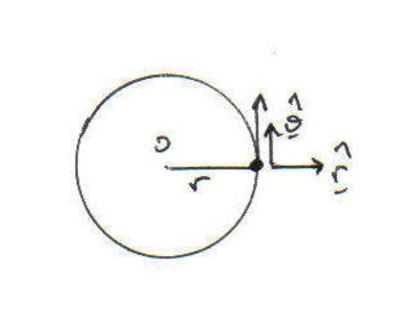
\includegraphics[scale=0.6]{notes/images/Circular-Motion.JPG}
    \caption{Motion in a circle}
    \label{fig:circular-motion}
\end{figure}
\FloatBarrier

From the definition of velocity, it also follows that the displacement $\vec{s}$ of the particle is given by
\begin{equation}
    \vec{s} = r \theta \hat{\theta}.
\end{equation}
We sometimes write the \textbf{angular velocity} as $\omega = \frac{\mathop{\mathrm{d}\theta}}{\mathop{\mathrm{d}t}} = \dot{\theta}$ which is measured in \textbf{radians per second} ($\text{rad} s^{-1}$), although revolutions per minute ($\text{rpm}$) is occasionally used, in which case
\begin{equation}
    \vec{v} = r \omega \hat{\theta}.
\end{equation}
The acceleration of the particle is given by
\begin{equation}
    \vec{a} = \left( -r\dot{\theta}^2\right) \hat{r} + r \ddot{\theta} \hat{\theta}.
\end{equation}
If the angular velocity is constant, it implies $\dot{\omega} = \ddot{\theta} = 0$, and 
\begin{equation}
    \vec{a} = -r \dot{\theta}^2 \hat{r} = -r \omega^2 \hat{r}.
\end{equation}
and the acceleration is directed towards the centre of the circle, since we only have the radial component $- r \omega^2$. Since $\vec{v} = r \omega \hat{\theta}$ with a magnitude of $\| \vec{v} \| = r \omega$ and so
\begin{equation}
    \vec{a} = - \frac{\| \vec{v} \|^2}{r} \hat{r}.
\end{equation}
This acceleration is called the \textbf{centripetal acceleration}. It follows from Newton's second law of motion that there \textit{must} exist a force $\vec{F}$, such that
\begin{equation}
    \vec{F} = m \vec{a} = - m r \omega^2 \hat{r} = - m \frac{\| \vec{v} \|^2}{r} \hat{r},
\end{equation}
which also acts radially, towards the centre of the circle and has the radial component of $- m r \omega^2$ or $- m \frac{\| \vec{v} \|^2}{r}$.

\subsection{Central forces}
\label{subsection:central-forces}
A \textbf{central force} is one which is purely radial (directed along a radius), either towards or away from the centre, such that
\begin{equation}
    \vec{F}(r) = F(r) \hat{r}.
\end{equation}
If $F(r)$ is positive, the force is said to be \textbf{repulsive} or \textbf{centrifugal}; whereas if $F(r)$ is negative the force is \textbf{attractive} or \textbf{centripetal}. 

Applying Newton's second law of motion and acceleration in plane polar coordinates yields the following equations of motion
\begin{equation}
    m\left[\left(\ddot{r} - r \dot{\theta}^2\right)\hat{r} + \left(2 \dot{r} \dot{\theta} + r \ddot{\theta}\right)\hat{\theta}\right] = F(r)\hat{r}
\end{equation}
We see that the force is entirely radial, so
\begin{align}
    m\left(\ddot{r} - r\dot{\theta}^2\right) &= F(r) \\
    m(2\dot{r}\dot{\theta} + r\ddot{\theta}) &= 0
\end{align}
We define the \textbf{magnitude} of \textbf{angular momentum}, $\| \vec{L} \|$ of a particle about a point $O$ as
\begin{equation}
    \| \vec{L} \| = mr \| \vec{v}_{\theta} \| = mr^2 \dot{\theta},
\end{equation}
where $\vec{v}_{\theta}$ is the transverse component of velocity in plane polar coordinates. Thus
\begin{align}
    \frac{\mathop{\mathrm{d}\| \vec{L} \|}}{\mathop{\mathrm{d}t}} &= m\left(2 r \dot{r} \dot{\theta} + r^2 \ddot{\theta}\right) \\
    &= mr\left(2\dot{r}\dot{\theta} + r \ddot{\theta}\right) \\
    &= mr\| \vec{a}_{\theta} \|,
\end{align}
where we denote the transverse acceleration as $\vec{a}_{\theta} = \left(2\dot{r}\dot{\theta} + r \ddot{\theta}\right) \hat{\theta}$. However, for a central force, the transverse acceleration is zero, so
\begin{equation}
    \frac{\mathop{\mathrm{d}\| \vec{L} \|}}{\mathop{\mathrm{d}t}} = 0,
\end{equation}
and hence the magnitude angular momentum $\| \vec{L} \|$ is constant during the motion of any central force.

\subsection{Rotating Frame of Reference}

Consider an observer $A$ standing on a rotating disk as shown in figure ??. 

The real force of friction at the feet provides the centripetal acceleration $-r\omega^2 \hat{r}$, therefore $\vec{F} = -mr\omega^2\hat{r}$. \textbf{Relative to the disk} the person is at \textbf{rest} under the influence of a real centripetal force and a \textbf{fictitious} \textbf{\textit{centrifugal force}} (\textit{yes, its exists!}) $\mathfrak{F}_{cent} = mr\omega^2\hat{r}$ acting through the centre of mass. 

\begin{example}{(\textbf{A Geostationary Satellite})}
Consider a geostationary satellite, a satellite that appears stationary relative to an observer on a rotating Earth as shown below.

The real force on the satellite is the gravitational force (centripetal force);
\begin{equation*}
    \vec{F} = - mr \omega^2 \hat{r}.
\end{equation*}
The observer on Earth thinks there is also a fictitious centrifugal force (by Newton's first law of motion),
\begin{equation*}
    \mathfrak{F}_{cent} = mr \omega^2 \hat{r}
\end{equation*}
so there is no resultant force, and so the satellite is at rest and in equilibrium with respect to this frame.
\end{example}

We discussed the relative positions of moving points in inertial reference frames in section ??, we will do the same for rotating frames of reference. Consider an observed $B$ at rest on a spinning disk observing a moving body, e.g. a flying bird, as shown in figure ??. Consider the same bird being observed by a second observer $A$ at rest relative to the Earth. The path of the bird, as observed by $A$, is a straight line, however, relative to observer $B$ the path of the bird is curved. So observer $B$ can assume there is a transverse horizontal force $\mathfrak{F}_{cor}$ acting on the bird, deflecting the bird to the right for the given sense of rotation. This is known as the \textbf{Coriolis force}, whose magnitude is given by
\begin{equation}
    \mathfrak{F}_{cor}  = - 2 m \dot{r} \omega \hat{\theta},
\end{equation}
where $\omega$ is the angular velocity of the rotating frame, $\dot{r}$ is the radial velocity and $m$ is the mass of the particle.

To find the Coriolis force, let us consider a massless smooth rod on which there is a disk of mass $m$. The rod is rotating with a constant angular velocity $\omega$ in a horizontal plane. As the rood is smooth there can be no radial force (from friction) on the pivot of the disk. The only force on the pivot is a transverse normal reaction force $\vec{F}_n$ as shown in the figure below. 


The equation of motion of the pivot is (relative to the inertial reference frame),
\begin{equation}
    m \vec{a} = \vec{F}_n
\end{equation}
\begin{equation}
    m \left[ \left(\ddot{r} - r \dot{\theta}^2 \right) \hat{r} + \left(2 \dot{r} \dot{\theta} + r \ddot{\theta}\right) \hat{\theta} \right] = \| \vec{F}_n \| \hat{\theta}
\end{equation}
Therefore the radial equation of motion is
\begin{equation}
    m \left(\ddot{r} - r \dot{\theta}^2 \right) \hat{r} = \vec{0}
\end{equation}
and the transverse one is
\begin{equation}
    m \left(2 \dot{r} \dot{\theta} + r \ddot{\theta} \right) \hat{\theta} = \| \vec{F}_n \| \hat{\theta}.
\end{equation}
But, we have a constant angular velocity, so $\ddot{\theta} = \dot{\omega} = 0$, giving us
\begin{equation}
    m \left(\ddot{r} - r \omega^2 \right) \hat{r} = \vec{0} 
\end{equation}
and
\begin{equation}
    2 m \dot{r} \omega \hat{\theta} = \| \vec{F}_n \| \hat{\theta}
\end{equation}

Now consider the equations of motion of the pivot relative to the rotating rod. In this frame the pivot can only move in on dimension along the rod. if we work in this frame we must add fictitious forces to the real forces, such as the fictitious centrifugal force $\mathfrak{F}_{cent}$ and the Coriolis force $\mathfrak{F}_{cor}$; as shown in figure ??

In the rotating frame the radial equation of motion is
\begin{equation}
    m \ddot{r} \hat{r} = \mathfrak{F}_{cent}
\end{equation}
and for the transverse component, we have
\begin{equation}
    \vec{F}_n + \mathfrak{F}_{cor} = \vec{0},
\end{equation}
as there is no transverse motion in the rotating frame. We can now compare the radial and transverse equations of motion in each frame to find the fictitious centrifugal and Coriolis forces. Comparing equation ?? with equation ?? gives the centrifugal force
\begin{equation}
    \mathfrak{F}_{cent} = m r \omega^2 \hat{r}
\end{equation}
and comparing equations ?? and ?? gives the Coriolis force
\begin{equation}
    \mathfrak{F}_{cor} = -2m\dot{r}\omega \hat{\theta}
\end{equation}

Despite this argument being mathematically valid, it isn't valid for 3 dimensions. In order to find the Coriolis force in 3 dimensions, we need to consider a pseudo surface-vector for angular velocity with respect to plane of rotation

\subsection{Torque}

\textbf{Torque} or \textbf{moments} are the rotational equivalent of linear force. Just as force can be thought as a push or a pull, a torque can be thought of as a twist to an object. We typically denote torque using $\vec{\tau}$. When referring to a moment of a force, it is more commonly denoted by $M$.

In three dimensions, the torque is a \textit{pseudo-vector}. It is given by the cross product of the radial vector and the force vector. So we have
\begin{equation}
    \vec{\tau} = \vec{r} \times \vec{F},
\end{equation}
where the magnitude is given by
\begin{equation}
    \| \vec{\tau}\| = \|\vec{r}\|\| \vec{F}\|\sin \theta,
\end{equation}
where $\theta$ is the angle between the force vector and the radial vector. The SI unit for torque is the \textbf{Newton metre} ($Nm$). The direction of torque is determined by the right-hand rule.

The unbalanced torque on a body along the axis of rotation determines the rate of change of the body's angular momentum. 

\begin{equation}
     \vec{\tau}  = \frac{\mathop{\mathrm{d} \vec{L} }}{\mathop{\mathrm{d}t}}.
\end{equation}

If multiple torques are acting on the body, it is instead the net torque which determines the rate of change of the angular momentum

\begin{equation}
    \vec{\tau}_1 + \cdots + \vec{\tau}_n = \vec{\tau}_{net}  = \frac{\mathop{\mathrm{d} \vec{L}}}{\mathop{\mathrm{d}t}}.
\end{equation}

The equivalence of angular momentum and torque can be proved easily by considering the following definition of angular momentum $\vec{L}$: 
\begin{equation}
    \vec{L} = \vec{r} \times \vec{p},
\end{equation}
where $\vec{r}$ is the radial vector and $\vec{p}$ is the particle's linear momentum. So the time derivative of this is
\begin{equation}
    \frac{\mathop{\mathrm{d}\vec{L}}}{\mathop{\mathrm{d}t}} = \vec{r} \times \frac{\mathop{\mathrm{d}\vec{p}}}{\mathop{\mathrm{d}t}} + \frac{\mathop{\mathrm{d}\vec{r}}}{\mathop{\mathrm{d}t}} \times \vec{p}
\end{equation}
From Newton's second law of motion we have $\vec{F} = \frac{\mathop{\mathrm{d}\vec{p}}}{\mathop{\mathrm{d}t}}$ and the definition of velocity (in rotational motion) is $\vec{v} = \frac{\mathop{\mathrm{d}\vec{r}}}{\mathop{\mathrm{d}t}}$. So
\begin{equation}
    \frac{\mathop{\mathrm{d}\vec{L}}}{\mathop{\mathrm{d}t}} = \vec{r} \times \vec{F} + \vec{v} \times \vec{p}
\end{equation}
The cross product of linear momentum $\vec{p}$ and velocity $\vec{v}$ is zero because velocity and momentum are parallel. So it follows that
\begin{equation}
    \frac{\mathop{\mathrm{d}\vec{L}}}{\mathop{\mathrm{d}t}} = \vec{r} \times \vec{F}_{net} = \vec{\tau}_{net}
\end{equation}

\subsubsection*{Rotational Work}
If a force acts through a distance, it is doing work. Similarly, if torque acts through a rotational distance, it is doing work. Mathematically, for rotation about a fixed axis through the centre of mass,
\begin{equation}
    W = \int_{\theta_1}^{\theta_2} \| \vec{\tau} \| \mathop{\mathrm{d}\theta}.
\end{equation}
Let us consider the definition of work done,
\begin{equation}
    W = \int_C \vec{F} \cdot \mathop{\mathrm{d}\vec{s}}
\end{equation}
However, for an infinitesimal displacement $\mathop{\mathrm{d}\vec{s}}$ is related to a corresponding angular displacement $\mathop{\mathrm{d}\vec{\theta}}$ and the radial vector $\vec{r}$ as
\begin{equation}
    \mathop{\mathrm{d}\vec{s}} = \mathop{\mathrm{d}\vec{\theta}} \times \vec{r}
\end{equation}
Substituting this into equation ?? yields
\begin{equation}
    W = \int_{\vec{\theta}_1}^{\vec{\theta}_2} \vec{F} \cdot (\mathop{\mathrm{d}\vec{\theta}} \times \vec{r})
\end{equation}
Notice the triple scalar product in the integrand above, which can be rewritten as
\begin{equation}
    W = \int_{\vec{\theta}_1}^{\vec{\theta}_2} (\vec{r} \times \vec{F}) \cdot \mathop{\mathrm{d}\vec{\theta}}
\end{equation}
From the definition of torque, we have
\begin{equation}
    W = \int_{\vec{\theta}_1}^{\vec{\theta}_2} \vec{\tau} \cdot \mathop{\mathrm{d}\vec{\theta}}
\end{equation}
Given torque and angular displacement are always parallel, then the scalar product simply reduces to a product of magnitudes, so
\begin{equation}
    W = \int_{\theta_1}^{\theta_2} \| \vec{\tau} \| \mathop{\mathrm{d}\theta}.
\end{equation}

\subsubsection*{The Principle of Moments}

The Principle of Moments, simply states that the sum of torques applied to a single point is equal to the torque due to the sum (resultant) of the forces. Mathematically, this is
\begin{equation}
    (\vec{r} \times \vec{F}_1) + (\vec{r} \times \vec{F}_2) + \cdots = \vec{r} \times (\vec{F}_1 + \vec{F}_2 + \cdots)
\end{equation}
A corollary of this is that for a body in rotational equilibrium the sum of the torques acting on the body is zero. 

However, in A2 Physics, we learn \textbf{wrong} Physics, so instead the Principle of Moments states that for a body in rotational equilibrium, the sum of the clockwise moments about any point is equal to the sum of anticlockwise moments about the same point 

\subsubsection*{Couples}

A \textbf{couple} refers to a pair of parallel forces that are equal in magnitude, but oppositely directed. The forces have a turning effect or moment called a torque above an axis which is perpendicular to the plane of the forces. 

FIGURE HERE

If the two forces are $\vec{F}$ and $-\vec{F}$, then the magnitude of the torque is given by
\begin{equation}
    \| \vec{\tau} \| = \| \vec{F} \| d
\end{equation}


\section{Planetary Motion}

\subsection{The Universal Law of Gravitation}

The universal law of gravitation, also know as \textbf{Newton's law of gravitation}, states that the magnitude of the \textbf{gravitational force} $\vec{F}$ between any two particles with masses $m_1$ and $m_2$ is proportional to the product of the two masses and inversely proportional to the square of their separation $r$.
\begin{equation*}
    \| \vec{F} \| \propto \frac{m_1 m_2}{r^2}.
\end{equation*}
The constant of proportionality is denoted as $G$, the \textbf{gravitational constant}. So we say the gravitational force $\vec{F}_{1,2}$ exerted on particle $1$ due to particle $2$ with masses $m_1$ and $m_2$ and position vectors $r_1$ and $r_2$ respectively is 
\begin{equation}
    \vec{F}_{1,2} = - \frac{G m_1 m_2}{\| \vec{r}_{2,1} \|^2} \hat{r}_{2,1}
    \label{eq:gravitational-force}
\end{equation}
and $\vec{r}_{2,1}$ is the separation vector pointing from particle 2 to particle 1, hence
\begin{equation}
    \hat{r}_{2,1} = \frac{\vec{r}_{2,1}}{\| \vec{r}_{2,1} \|} \text{ and } \vec{r}_{2, 1} = \vec{r}_1 - \vec{r}_2.
\end{equation}
We note that by Newton's third law of motion, the force on the particle with $m_2$ exerted by $m_1$ is given by
\begin{equation}
    \vec{F}_{2, 1} = -\vec{F}_{1, 2}.
\end{equation}

The gravitational force is an example of a \textbf{central force} (See section \ref{subsection:central-forces}).

\begin{figure}[h!]
    \centering
    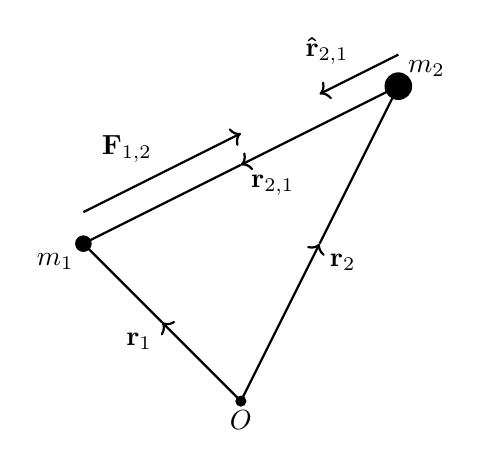
\begin{tikzpicture}
        \coordinate (O) at (0,0);
        \coordinate (A) at (2,4);
        \coordinate (B) at (-2,2);
        
        \fill (O) circle[radius=2pt] node[below] {$O$};
        \fill (A) circle[radius=5pt] node[above right] {$m_2$};
        \fill (B) circle[radius=3pt] node[below left] {$m_1$};
        
        \draw[->, thick] (O) -- (-1,1) node[below left] {$\vec{r}_1$};
        \draw[thick] (-1,1) -- (B);
        \draw[->, thick] (O) -- (1,2) node[below right] {$\vec{r}_2$};
        \draw[thick] (1,2) -- (A);
        
        \draw[->, thick] (-2,2.4) -- (0,3.4) node[midway, above left] {$\vec{F}_{1,2}$};
        \draw[->, thick]  (A) -- (0,3) node[below right] {$\vec{r}_{2,1}$};
        \draw[thick] (0,3) -- (B);
        
        \draw[->, thick] (2,4.4) -- (1,3.9) node[midway, above left] {$\hat{r}_{2,1}$};
    \end{tikzpicture}
    \caption{Vector diagram showing the geometry of the gravitational attraction}
\end{figure}
\FloatBarrier

\subsection{Gravitational Fields}

While two particles are needed to produce a gravitational force, a \textbf{gravitational field} for any single particle in space is used to describe it's effect on other particles. We say a particle $p$ in space produces a gravitation field $\vec{g}$ with spherical symmetry. We have
\begin{equation}
    \label{eq:gravitational-field-1}
    \vec{g} = - \frac{Gm_1}{\| \vec{r} \|^2} \hat{r}
\end{equation}
and so we have
\begin{equation}
    \label{eq:gravitational-field-2}
    \vec{g} = \frac{\vec{F}}{m_2}
\end{equation}
where $\hat{r}$ is a unit surface vector and $\vec{r}$ is a radial vector that is always perpendicular to the surface of the particle. So $\vec{r}$ is always pointing away from the particle towards other particles. In field theory, we represent a gravitational field as a vector field, however, in this course we will use \textit{field lines} to represent the gravitational field.

\begin{figure}[h!]
    \centering
    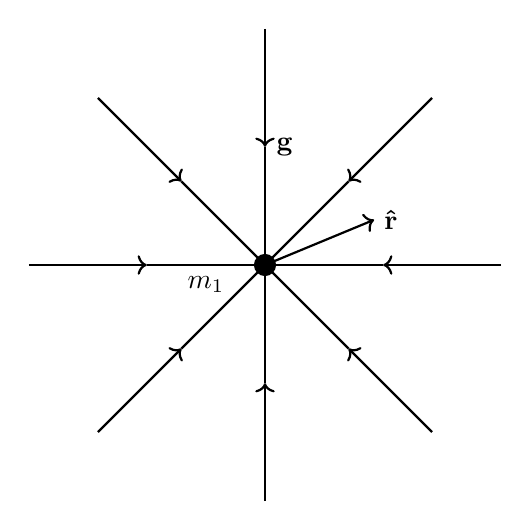
\begin{tikzpicture}
        \coordinate (O) at (0,3);

        
        \fill (O) circle[radius=4pt];
        
        \node at (-0.75,2.75) {$m_1$};
        
        \foreach \i in {1,...,8} {
            \pgfmathsetmacro{\cosValue}{cos(\i * 45)};
            \pgfmathsetmacro{\sinValue}{sin(\i * 45)};
            \draw[->, thick] (3 * \cosValue, 3 * \sinValue + 3) -- (1.5 * \cosValue,1.5 * \sinValue + 3);
            \draw[thick] (1.5 * \cosValue,1.5 * \sinValue + 3) -- (0,3);
        }
        
        \node at (0.25,4.5) {$\vec{g}$};
        \pgfmathsetmacro{\cosValue}{cos(22.5)};
        \pgfmathsetmacro{\sinValue}{sin(22.5)};
        \draw[->, thick] (0,3) -- (1.5 * \cosValue,1.5 * \sinValue + 3) node[at end, right] {$\hat{r}$};
    \end{tikzpicture}
    \caption{Vector diagram showing the geometry of the gravitational field}
\end{figure}
\FloatBarrier

The figure above shows a radial gravitational field of a particle. A \textbf{uniform gravitational field} is said to have field lines that are parallel and equidistant. The field at the surface of the particle is \textit{approximately} uniform. 

\begin{figure}[h!]
    \centering
    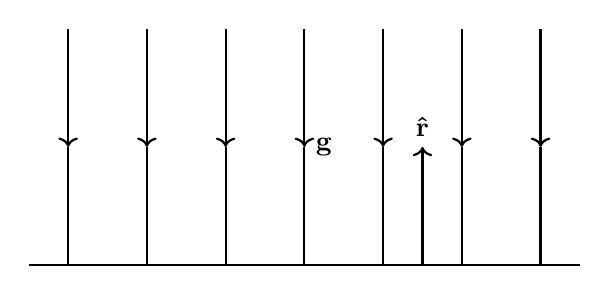
\begin{tikzpicture}
        \draw[thick] (-3.5,0) -- (3.5,0);
        
        \foreach \i in {-3,...,3} {
            \draw[->, thick] (\i,3) -- (\i,1.5);
            \draw[thick] (\i,1.5) -- (\i,0);
        }
        
        \node at (0.25,1.5) {$\vec{g}$};
        \draw[->, thick] (1.5,0) -- (1.5,1.5) node[at end, above] {$\hat{r}$};
    \end{tikzpicture}
    \caption{Vector diagram showing the geometry of a uniform gravitational field}
\end{figure}
\FloatBarrier

In this course, we denote the gravitational field strength $\| \vec{g} \|$ as the magnitude of the gravitational field, however, we say that 
\begin{equation}
    \label{eq:gravitational-field-strength}
    \| \vec{g} \| = - \frac{Gm_1}{\| \vec{r} \|^2}.
\end{equation}
We use a negative sign to infer that the gravitational field is an \textbf{attractive} force, so it has the direction $-\hat{r}$. This isn't common practice, since magnitudes are always positive, however this is an exception in this course. 

\subsection{Gravitational Potential Energy}

By virtue of it's position in the gravitational field $\vec{g}$ due to mass $m_1$, any mass $m_2$ has \textbf{gravitational potential energy}. We can consider the change in potential $\Delta E_p$ by considering the work done moving a mass $m_2$ from positions 1 to 2, that is
\begin{equation}
    \Delta E_p = \int_C \vec{F} \cdot \mathop{\mathrm{d}\vec{r}}
\end{equation}
Applying equation \ref{eq:gravitational-force}, we find 
\begin{align}
    \Delta E_p &= \int_C - \frac{G m_1 m_2}{\| \vec{r} \|^2} \hat{r} \cdot \mathop{\mathrm{d}\vec{r}} \\
    &= - G m_1 m_2 \int_C \frac{\hat{r}}{\| \vec{r} \|^2} \cdot \mathop{\mathrm{d}\vec{r}}
\end{align}
Note that $\hat{r} \cdot \mathop{\mathrm{d}\vec{r}} = \mathop{\mathrm{d}r}$, so we don't need to consider a tangential vector to the curve $C$, also the gravitational field is a \textbf{conservative field}, so the mass $m$ being moved from $r_1$ to $r_2$ is not relevant to the work done, which only depends on the initial and final positions. Hence
\begin{align}
    \Delta E_p &= -G m_1 m_2 \int_{r_1}^{r_2} \frac{1}{r^2} \mathop{\mathrm{d}r} \\ 
    &= -Gm_1m_2 \left(\frac{1}{r_2} - \frac{1}{r_1}\right)
\end{align}
One often takes a reference point at $r_{ref} = \infty$ such that the gravitational potential energy is zero at $r_{ref}$, that is $E_p(r_{ref}) = 0$. Thus
\begin{equation}
    E_p(r_{ref}) - E_p(r) = -Gm_1m_2 \left(\frac{1}{r_{ref}} - \frac{1}{r}\right), \\
\end{equation} 
so we have,
\begin{equation}
    E_p(r) = - \frac{G m_1 m_2}{r}.
\end{equation}

\subsection{Gravitational Potential}
In general for a gravitational field, the \textbf{gravitational potential} $V$ is defined as 
\begin{equation}
    V = \frac{E_p}{m_2} = - \frac{G m_1}{r}
\end{equation}
where $m_1$ is a fixed particle and $m_2$ is the so-called test particle (or point mass). It is the work done per unit of mass. Using our definition of gravitational field strength (see equation \ref{eq:gravitational-field-2}), we have
\begin{equation}
    V = \| \vec{g} \| r.
\end{equation}
Recalling the definition of a gravitational field $\vec{F} = m_2 \vec{g}$ and gravitational potential energy (see equation \ref{eq:gravitational-field-strength}), so
\begin{align}
    \Delta V &= \frac{1}{m_2} \int_C \vec{F} \cdot \mathop{\mathrm{d}\vec{r}} \\
    &= \int_C \vec{g} \cdot \mathop{\mathrm{d}\vec{r}}
\end{align}
This is known as the \textbf{potential difference} in a gravitational field, evaluating line integral above yields the following relation for potential difference,
\begin{equation}
    \Delta V = - G m_1 \left(\frac{1}{r_2} - \frac{1}{r_1}\right),
\end{equation}
where $r_1$ and $r_2$ denote the initial and final positions of the test particle respectively. Following the same convention that we used for gravitational potential energy - the \textbf{potential well} convention, we consider the potential with respect to some reference point $r_{ref}$ such that the potential is zero at $r_{ref}$. So we have
\begin{equation}
    V(r) = - \frac{G m_1}{r}
\end{equation}

The potential is the integration over space, specifically a line (since we used a line integral), of a field. Vice versa, the gravitational field is the spatial derivative of the potential.     
\begin{equation}
    \vec{g} = -\frac{Gm_1}{\| \vec{r} \|^2}\hat{r} = \frac{\partial}{\mathop{\partial \vec{r}}} \frac{G m_1}{\| \vec{r} \|} = - \nabla V.
\end{equation}
We can prove these via the following argument. Firstly, considering the partial derivative of $G m_1 / \| \vec{r} \|$ with respect to $\vec{r}$ in $\mathbb{R}^3$. Applying our vector calculus knowledge, we find that
\begin{align*}
    \frac{\partial}{\mathop{\partial \vec{r}}} \frac{G m_1}{\| \vec{r} \|} &= \left\langle
        \frac{\partial}{\partial r_1} \frac{G m_1}{\| \vec{r} \|} ,
        \frac{\partial}{\partial r_2} \frac{G m_1}{\| \vec{r} \|} ,
        \frac{\partial}{\partial r_3} \frac{G m_1}{\| \vec{r} \|}
    \right\rangle \\
    &= \left\langle
        - \frac{G m_1}{\| \vec{r} \|^2} \frac{r_1}{\| \vec{r} \|} ,
        - \frac{G m_1}{\| \vec{r} \|^2} \frac{r_2}{\| \vec{r} \|} ,
        - \frac{G m_1}{\| \vec{r} \|^2} \frac{r_1}{\| \vec{r} \|}
    \right\rangle  \\
    &= - \frac{G m_1}{\| \vec{r} \|^2} \hat{r}
\end{align*}
Now the spatial derivative (gradient) of the potential. We may easily see this in a more general way by expressing $\mathop{\mathrm{d}\vec{r}}$ as a vector in $\mathbb{R}^3$, using some of the properties of the dot product, we find that
\begin{equation*}
    \mathop{\mathrm{d}V} = \vec{g} \cdot \mathop{\mathrm{d}\vec{r}}
\end{equation*}
By definition, moving parallel to $\vec{g}$ produces a negative change in potential, hence
\begin{equation}
    \label{eq:del-potential-1}
    \mathop{\mathrm{d}V} = -\left(g_x \mathop{\mathrm{d}x} + g_y \mathop{\mathrm{d}y} + g_z \mathop{\mathrm{d}z}\right)
\end{equation}
We also know, from partial differentiation, that the total differential $\mathop{\mathrm{d}V}$ is given by
\begin{equation}
    \label{eq:del-potential-2}
    \mathop{\mathrm{d}V} = \frac{\partial V}{\partial x}\mathop{\mathrm{d}x} + \frac{\partial V}{\partial y}\mathop{\mathrm{d}y} + \frac{\partial V}{\partial z}\mathop{\mathrm{d}z}.
\end{equation}
Comparing equations \ref{eq:del-potential-1} and \ref{eq:del-potential-2} gives
\begin{equation}
    \vec{g} = - \left\langle \frac{\partial U}{\partial x}, \frac{\partial U}{\partial y}, \frac{\partial U}{\partial z} \right\rangle = - \nabla V.
\end{equation}

\subsection{Orbits}

Motion in orbits is due to motion under an inverse square law, which we will extensively analyze in this course due to planetary motion under the force of gravity (which exhibits an inverse square law). However, this is also applicable to electrostatic forces (such as electrons orbiting protons). The central force in gravitation or electrostatics is in the form
\begin{equation}
    \vec{F} = \frac{k}{\| \vec{r} \|^2} \hat{r},
\end{equation}
where $k$ is the coefficient of attraction (this allows us to generalize for gravitational and electric fields). If $k$ is positive the force is repulsive, if $k$ is negative the force is attractive. For the gravitational force, $k = -Gm_1m_2$ and for the electrostatic force $k = k_e q_1 q_2$ (see section ??). Representing the particle motion in plane polar coordinates, produces the following equation of motion 
\begin{equation}
    \label{eq:orbits-motion-1}
    m \left[\left(\ddot{r} - r \dot{\theta}^2\right)\hat{r} + \left(2\dot{r}\dot{\theta} + r \ddot{\theta}\right)\right] = \frac{k}{r^2}\hat{r}
\end{equation}
So we have the radial component
\begin{equation}
    m\left(\ddot{r} - r \dot{\theta}^2\right) = \frac{k}{r^2}
\end{equation}
and the transverse component
\begin{equation}
    \left(2 \dot{r} \dot{\theta} + r \ddot{\theta}\right) = 0.
\end{equation}

We note that earlier that
\begin{equation*}
    \frac{\mathop{\mathrm{d}\| \vec{L} \|}}{\mathop{\mathrm{d}t}} = 0 
\end{equation*}
when $\left(2 \dot{r} \dot{\theta} + r \ddot{\theta}\right) = 0$ (see section \ref{subsection:central-forces}). So we can write $\dot{\theta}$ in terms of the magnitude of angular momentum, hence
\begin{equation}
    \label{eq:theta-dot-angular-momentum}
    \dot{\theta} = \frac{\| \vec{L} \|}{m r^2},
\end{equation}
implying the radial component can be written as 
\begin{equation}
    m \left(\ddot{r} - \frac{\| \vec{L} \|^2}{m^2 r^3}\right) = \frac{k}{r^2}
\end{equation}
Instead of solving for $r$ and $\theta$, we will consider the shape of the orbit by considering $r$ as a function of $\theta$. To do this we define $u = 1/r$, so we have
\begin{align*}
    \dot{r} &= \frac{\mathrm{d}}{\mathop{\mathrm{d}t}} \left(\frac{1}{u}\right) \\
    &= - \frac{1}{u^2} \frac{\mathop{\mathrm{d}u}}{\mathop{\mathrm{d}\theta}} \frac{\mathop{\mathrm{d}\theta}}{\mathop{\mathrm{d}t}}
\end{align*}
Note that we have an expression for $\frac{\mathop{\mathrm{d}\theta}}{\mathop{\mathrm{d}t}}$ from equation \ref{eq:theta-dot-angular-momentum}, thus
\begin{equation}
    \label{eq:r-dot-L-theta}
    \dot{r} = - \frac{\| \vec{L} \|}{m} \frac{\mathop{\mathrm{d}u}}{\mathop{\mathrm{d}\theta}}.
\end{equation}
Differentiating again, we get
\begin{align}
    \ddot{r} &= \frac{\mathrm{d}}{\mathop{\mathrm{d}t}} \left( - \frac{\| \vec{L} \|}{m} \frac{\mathop{\mathrm{d}u}}{\mathop{\mathrm{d}\theta}}\right) \\
    &= \frac{\mathrm{d}}{\mathop{\mathrm{d}\theta}} \left( - \frac{\| \vec{L} \|}{m} \frac{\mathop{\mathrm{d}u}}{\mathop{\mathrm{d}\theta}}\right) \frac{\mathop{\mathrm{d}\theta}}{\mathop{\mathrm{d}t}} \\
    &= - \left(\frac{u\| \vec{L} \|}{m}\right)^2 \frac{\mathop{\mathrm{d}^2u}}{\mathop{\mathrm{d}\theta^2}}
    \label{eq:r-2dot-L-theta}
\end{align}
Writing equation \ref{eq:orbits-motion-1} in terms of $u$, yields
\begin{equation}
    m \left[- \left(\frac{u\| \vec{L} \|}{m}\right)^2 \frac{\mathop{\mathrm{d}^2u}}{\mathop{\mathrm{d}\theta^2}} - \frac{u^3 \| \vec{L} \|^2}{m^2}\right] = ku^2.
\end{equation}
Simplifying gives
\begin{equation}
    \label{eq:orbits-motion-2}
    \frac{\mathop{\mathrm{d}^2u}}{\mathop{\mathrm{d}\theta^2}} + u = - \frac{km}{\| \vec{L} \|^2}.
\end{equation}
If we let $\lambda = u + km/\| \vec{L} \|^2$, then we get
\begin{equation}
    \frac{\mathop{\mathrm{d}^2\lambda}}{\mathop{\mathrm{d}\theta^2}} + \lambda = 0,
\end{equation}
which is a special case of the second order linear differential equation we solved for harmonic motion in section ?? with solution $\lambda = A \cos (\theta + \theta_0)$. Thus the general solution of equation \ref{eq:orbits-motion-2} is
\begin{equation}
    u  = \frac{1}{r} = A \cos(\theta + \theta_0) - \frac{km}{\| \vec{L} \|^2}
\end{equation}
This is in the same form as the general equation of \textbf{conic sections}
\begin{equation}
    u = \frac{1}{r} = \frac{1}{h} (1 + e \cos \theta),
\end{equation}
implying \textit{all trajectories can be modelled as \textbf{conic sections}}.  

A particle is said to be in \textbf{orbit} if it cannot escape to infinity on the trajectory modelled by a conic section. This implies that all orbits are elliptical with a special case of a circular orbit. 

\subsection{Conics}

A conic section is a locus of points which moves in a plane such that the ratio of its distance from a fixed point $r$, the focus, to the distance from a fixed straight line $x$, the directrix, is a constant $e$, the eccentricity.
\begin{equation}
    e = \frac{r}{x}
\end{equation}

\begin{figure}[h!]
    \centering
    \begin{tikzpicture}
        \tikzset{swapaxes/.style = {rotate=90,yscale=1}}
        
        \draw[->] (-4,0)--(8,0);
        \draw[->] (-3,-4)--(-3,4);
        \draw[swapaxes,thick] plot[domain=-2:2,smooth,variable=\y] ({-2 * \y}, {\y*\y});
        \fill (-0.5,1.414) circle[radius=2pt];
        \fill (-3,0) circle[radius=2pt] node[below left] {$\text{focus}$};
        \draw[->, thick, arrows={-latex}] (-3,0) -- (-0.5,1.414) node[midway, above left] {$r$};
        \draw[dashed] (6,-4) -- (6,4) node[pos=0.6 ,right] {$\text{directrix}$};
        \draw[->, thick, arrows={-latex}] (6, 1.414) -- (-0.5, 1.414) node[midway, above] {$x$};
        \draw[->, thick, arrows={-latex}] (6, 3.464) -- (-3, 3.464) node[midway, above] {$x_h$};
        \draw[->, thick, arrows={-latex}] (-3,0) -- (-3, 3.464) node[midway, left] {$h$};
        \fill (-3,3.464) circle[radius=2pt];
        \draw[thick] (-2,0) arc [start angle=0, end angle=29.5, radius=1] node[midway, pos=0.7, right] {$\theta$};
    \end{tikzpicture}
    \caption{Conic section}
    \label{fig:conic-section}
\end{figure}
\FloatBarrier


Consider the conic section shown above. The quantity $h$ is the value of $r$ when $\theta  = \pi / 2$. Using simple geometry, we see that
\begin{equation}
    r \cos \theta + x = x_h,
\end{equation}
where $x$ is the distance from the directrix to the point and $x_h$ is the distance from the directrix to the point when $r = h$, as illustrated in figure \ref{fig:conic-section}. Using the definitions of $h$ and $e$, yields
\begin{equation}
    r \cos \theta + \frac{r}{e} = \frac{h}{e},
\end{equation}
and so
\begin{equation}
    \label{eq:conic}
    r (1 + e \cos \theta) = h
\end{equation}

\begin{table}[h!]
    \centering
    {
        \begin{tabular}{c|c}
            Conic Section & Eccentricity  \\
            \hline
            Circle & $e = 0$ \\
            Ellipse & $0 < e < 1$ \\
            Parabola & $e = 1$ \\ 
            Hyperbola & $e > 1$
        \end{tabular}
    }
\end{table}
\FloatBarrier

However, this gives us no physical intuition into the type of trajectories a particle may have. Trajectories are based (as we shall see later) on the total energy of the particle. Given we're discussing planetary motion, it is sensible to only consider the attractive force of gravitation / electrostatics (as we are not required to model the trajectories of proton-to-proton or electron-to-electron interactions) on a particle. 

\subsubsection{Trajectories - Attractive forces}
\begin{enumerate}
    \item If the total energy $E > 0$ and the eccentricity $e > 1$ the trajectory is a hyperbola.
    \item If the total energy is zero and eccentricity is one, $E = 0 \text{ and } e = 1$, then the trajectory is a parabola.
    \item If the total energy $E < 0$ and the eccentricity $e < 1$, the trajectory is an ellipse. The particle is said to have an elliptical orbit. 
    \item If the total energy $E < 0$ and the eccentricity is zero $e = 0$, then we have a circular trajectory (\textit{a special case of an ellipse with zero eccentricity}). The particle is said to have a circular orbit.
\end{enumerate}


\subsubsection{Determination of Eccentricity}

We shall determine the eccentricity of a trajectory based of a given total energy and magnitude of angular momentum $\| \vec{L} \|$. First let us define the total energy of a particle $E$, such that
\begin{equation}
    \label{eq:total-energy-1}
    E = E_k + E_p = \frac{1}{2}m\| \vec{v} \|^2 + \frac{k}{r}
\end{equation}
and is constant throughout the motion (gravitational and electric forces are conservative). So applying equation \ref{eq:polar-speed} to \ref{eq:total-energy-1}, gives
\begin{equation}
    E = \frac{1}{2}m\left(\dot{r}^2 + r^2 \dot{\theta}^2\right) + \frac{k}{r},
\end{equation}
however we have relations for $\dot{r}$ and $\dot{\theta}$ in terms of $u$ and $\| \vec{L} \|$ (see equations \ref{eq:r-dot-L-theta} and \ref{eq:r-2dot-L-theta}), so
\begin{align}
    E &= \frac{1}{2} m \left[\frac{\| \vec{L}\|^2}{m^2} \left(\frac{\mathop{\mathrm{d}u}}{\mathop{\mathrm{d}\theta}}\right)^2 + \frac{1}{u^2} \left(\frac{\| \vec{L} \|}{m}u^2\right)^2\right] + ku \\
    &= \frac{1}{2}\frac{\| \vec{L} \|^2}{m} \left[\left(\frac{\mathop{\mathrm{d}u}}{\mathop{\mathrm{d}\theta}}\right)^2 + u^2\right] + ku.
\end{align}
From this, we can infer that
\begin{enumerate}
    \item If $k > 0$, then $E > 0$.
    \item If $k < 0$, the $E \in \mathbb{R}$, that is to say $E$ may be positive, zero or negative.
\end{enumerate}

\noindent The equation of an orbit is 
\begin{equation*}
    u = A \cos (\theta + \theta_0) - \frac{km}{\| \vec{L} \|^2},
\end{equation*}
so 
\begin{equation}
    \frac{\mathop{\mathrm{d}u}}{\mathop{\mathrm{d}\theta}} = -A\sin (\theta + \theta_0).
\end{equation}
If we now let $\theta_0 = 0$ (for convenience), as this only defines the orientation of the trajectory of the particle, and therefore can be arbitrary. And so the expression for the total energy becomes
\begin{align}
    E &= \frac{1}{2} \frac{\| \vec{L} \|^2}{m} \left(A^2 \sin^2 \theta + A^2 \cos^2 \theta - 2 \frac{Akm}{\| \vec{L} \|^2}\cos \theta + \frac{k^2 m^2}{\| \vec{L} \|^4} \right) + k\left(A \cos \theta - \frac{km}{\| \vec{L} \|^2}\right) \\ 
    &= \frac{1}{2} \frac{\| \vec{L} \|^2}{m} \left(A^2 - 2 \frac{Akm}{\| \vec{L} \|^2}\cos \theta + \frac{k^2 m^2}{\| \vec{L} \|^4} \right) + k\left(A \cos \theta - \frac{km}{\| \vec{L} \|^2}\right)
\end{align}
Energy is conserved throughout the motion, so we can evaluate the expression for $E$ at any convenient point. We choose $\theta = \pi/2$, so
\begin{align}
    E &= \frac{1}{2} \frac{\| \vec{L} \|^2}{m} \left(A^2 + \frac{k^2 m^2}{\| \vec{L} \|^2}\right) - \frac{k^2m}{\| \vec{L} \|^2} \\ 
    &= \frac{A^2 \| \vec{L} \|^2}{2m} + \frac{k^2 m}{2 \| \vec{L} \|^2} - \frac{k^2m}{\| \vec{L}\|^2} \\
    &= \frac{A^2 \| \vec{L} \|^2}{2m} - \frac{k^2 m}{2 \| \vec{L} \|^2}
\end{align}
Rearranging this to determine the arbitrary constant $A$ yields
\begin{align}
    A^2 &= \frac{2m}{\| \vec{L} \|^2} \left(E + \frac{k^2m}{2 \| \vec{L} \|^2}\right) \\
    &= \frac{m}{\| \vec{L} \|^4} \left(k^2 m + 2 E \| \vec{L} \|^2\right) \\
    &= \frac{k^2 m^2}{\| \vec{L} \|^4} \left(1 + \frac{2E\|\vec{L}\|^2}{k^2m}\right)
\end{align}
and so
\begin{equation}
    A = \frac{\left|k\right|m}{\| \vec{L} \|^2} \sqrt{1 + \frac{2 E \| \vec{L} \|^2}{k^2m}}
\end{equation}
So the orbit can be determined if the values of $E$ and $\| \vec{L}\|$ are known for a given $k$ and $m$. The orbit is given by
\begin{equation}
    u = A \cos \theta - \frac{km}{\| \vec{L} \|^2}
\end{equation}
and the general form of a conic section is
\begin{align*}
    u &= \frac{1}{h} (1 + e\cos \theta) \\
    &= \frac{e}{h} \cos \theta + \frac{1}{h}
\end{align*}
So comparing coefficients produces
\begin{align}
    \frac{e}{h} &= A \\
    \frac{1}{h} &= - \frac{km}{\| \vec{L} \|^2}
    \label{eq:conic-h}
\end{align}
hence
\begin{align}
    e = Ah &= - \frac{\| \vec{L} \|^2}{km} \frac{\left|k\right|m}{\| \vec{L} \|^2} \sqrt{1 + \frac{2 E \| \vec{L} \|^2}{k^2m}} \\
    &= - \frac{|k|}{k} \sqrt{1 + \frac{2 E \| \vec{L} \|^2}{k^2m}}
\end{align}
For an attractive inverse square law force such as gravitation $k$ is negative so
\begin{equation}
    \label{eq:conic-e}
    e = \sqrt{1 + \frac{2 E \| \vec{L} \|^2}{k^2m}}
\end{equation}
Clearly
\begin{enumerate}
    \item If $E > 0$, then $e > 0$ so the trajectory is a hyperbola
    \item If $E = 0$, then $e = 1$ so the trajectory is a parabola
    \item If $E < 0$, then $e < 0$ so the trajectory is a ellipse. In this case, we say the particle in in \textbf{orbit}. As the particle cannot escape to infinity since $V = 0$ at $r = \infty$ and the kinetic energy is always greater than or equal to zero. Therefore to escape to infinity requires $E \geq 0$.
\end{enumerate}

\subsubsection{Elliptical Orbits}

Since elliptical trajectories are the only possible type of orbits, we can independently analyze them. Consider an elliptic orbit, as illustrated below.

\begin{figure}[h!]
    \centering
    \begin{tikzpicture}
        \draw[dashed] (-6.5,0)--(6.5,0) node[above] {$\text{major axis}$};
        \draw[dashed] (0,-4)--(0,4) node[right] {$\text{minor axis}$};
        \draw[thick] (0,0) ellipse (5 and 3);
        \fill (2,0) circle[radius=2pt] node[above] {$\text{focus}$};
        \draw[->, thick, arrows={-latex}] (2.1,-0.2) -- (5,-0.2) node[midway, below] {$\vec{r}_A$};
        \fill (5,0) circle[radius=2pt] node[below right] {$A$};
        \draw[->, thick, arrows={-latex}] (1.9,-0.2) -- (-5,-0.2) node[midway, below] {$\vec{r}_B$};
        \fill (-5,0) circle[radius=2pt] node[below left] {$B$};
        \draw[latex'-latex',double] (0,0.6) -- (5,0.6) node[midway, above] {$a$};
        \draw[->, thick, arrows={-latex}] (5,0) -- (5,2) node[midway, right] {$\vec{v}_A$};
        \draw[latex'-latex',double] (-5,-4.5) -- (5,-4.5) node[midway, below] {$2a$};
        \draw[->, thick, arrows={-latex}] (-5,0) -- (-5,-2) node[midway, left] {$\vec{v}_B$};
    \end{tikzpicture}
    \caption{Parameters for an elliptical orbit.}
\end{figure}
\FloatBarrier

If we know the velocity of the particle $\| \vec{v}_A \|$ at the position of closest approach $\vec{r}_A = r_A \hat{r}$ (when $\theta = 0$), we know everything about the orbit. The magnitude of angular momentum is
\begin{equation}
   \| \vec{L} \| = m r_A \| \vec{v}_A \| 
\end{equation}
and the energy is
\begin{equation}
    E = \frac{1}{2}m \| \vec{v}_A \|^2 - \frac{|k|}{r_A}.
\end{equation}
We can determine the eccentricity $e$ and the length of the \textit{semi-major axis} $a$ from the equation
\begin{equation*}
    r(1 + e \cos \theta) = h.
\end{equation*}
We have for $\vec{r}_A = r_A \hat{r}$ (when $\theta = 0$) and $\vec{r}_B = r_B \hat{r}$ (when $\theta = \pi$), so
\begin{equation}
    r_A(1 + e) = h \text{ and } r_B (1- e) = h,
\end{equation}
giving
\begin{align}
    2a &= r_A + r_B = \frac{2h}{1-e^2}, \\
    a &= \frac{h}{1-e^2}.
\end{align}
Substituting equations \ref{eq:conic-h} and \ref{eq:conic-e} into the expression above, produces
\begin{equation}
    a = \frac{- \frac{\| \vec{L} \|^2}{mk}}{- \frac{2E\| \vec{L} \|^2}{mk^2}} = \frac{k}{2E} = \left| \frac{k}{2E} \right|
\end{equation}
For a gravitational force exerted on the Earth due to the Sun, we say that point $A$ is the \textbf{perihelion} and point $B$ is the \textbf{aphelion}. These terms only apply if the \textit{Sun is at the focus}.

If the origin of the position vectors is taken at the mid-point of the \textit{major axis}, the focus is at position $\vec{r}_F = \langle ae, 0 \rangle$ and the Cartesian equation for the orbit is
\begin{equation}
    \frac{x^2}{\left[\frac{h^2}{(1-e^2)^2}\right]} + \frac{y^2}{\left[\frac{h^2}{1-e^2}\right]} = 1,
\end{equation}
or more commonly written as
\begin{equation}
    \frac{x^2}{a^2} + \frac{y^2}{b^2} = 1,
\end{equation}
with
\begin{equation}
    a = \frac{h}{1 - e^2} \text{ and } b = \frac{h}{\sqrt{1-e^2}},
\end{equation}
where $a$ and $b$ denote the lengths of the semi-major and semi-minor axes respectively. 

\subsection{Kepler's Laws of Planetary Motion}

Kepler's laws of planetary motion state that
\begin{enumerate}
    \item Planets move in elliptic orbits with the Sum at a focus, which we have proved in the previous sections.
    \item The radius vector sweeps out equal areas in equal times as illustrated below.
    
    \begin{figure}[h!]
        \centering
        \def\orbit{(1.5,0) ellipse(2.5cm and 2cm)}
        \begin{tikzpicture}[scale=2]
            \fill (0,0) coordinate (O) circle (2pt) node[below =7pt] {Sun};%
            \coordinate (A1) at (50.992527:5);
            \coordinate (A2) at (41.913511:5);
            \coordinate (B1) at (136.450216:5);
            \coordinate (B7) at (-150.524111:5);
            \coordinate (C1) at (-23.749494:5);
            \coordinate (C2) at (-18.581735:5);
            \coordinate (P) at (3.42,1.28);%%
            \fill (P) circle (1pt) node[above right] {Planet};%
            
            \begin{scope}  % The blue shaded regions
              \clip \orbit;
              \filldraw[fill=blue,opacity=0.5] (O) -- (A1) -- (A2) -- cycle;
              \filldraw[fill=blue,opacity=0.5] (O) -- (B1) -- (B7) -- cycle;%
              \filldraw[fill=blue,opacity=0.5] (O) -- (C1) -- (C2) -- cycle;%
              \end{scope}
            
              % The ellipse
            \draw \orbit;
            
            \draw (1.5,0) coordinate (M) --node[above]{\footnotesize $a$}  (4,0);
            \fill (M) circle (1pt);
        \end{tikzpicture}
        \caption{Kepler's second law}
    \end{figure}
    \FloatBarrier
    
    From figure \ref{fig:keplers-second-law}, the area of the triangle is
    \begin{equation}
        \mathop{\mathrm{d}A} = \frac{1}{2} r v_{\theta} \mathop{\mathrm{d}t}
    \end{equation}
    where $v_{\theta}$ is the transverse component of velocity in plane polar coordinates, so
    \begin{align}
        \mathop{\mathrm{d}A} &= \frac{1}{2} r^2 \dot{\theta} \mathop{\mathrm{d}t} \\
        \frac{\mathop{\mathrm{d}A}}{\mathop{\mathrm{d}t}} &= \frac{1}{2} r^2 \dot{\theta} \\
        &= \frac{1}{2} \frac{\| \vec{L} \|}{m}.
    \end{align}
    Since $\| \vec{L} \|$ is constant under any central force (such as gravitation), it implies that $\dot{A}$ is constant. Hence we have Kepler's second law.
    
    \begin{figure}[h!]
        \centering
        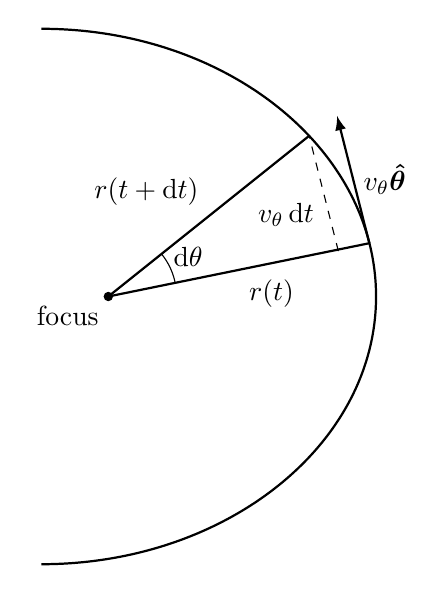
\begin{tikzpicture}[scale=0.85]
            \draw[rotate=180, thick] (0,-4) arc(270:90:5 and 4);
            \fill (1,0) circle[radius=2pt] node[below left] {focus};
            \draw[thick] (1,0) -- (4.9, 0.796) node[midway, below right] {$r(t)$};
            \draw[thick] (1,0) -- (4, 2.4) node[midway, above left] {$r(t + \mathop{\mathrm{d}t})$};
            \draw[thick, ->, arrows={-latex}] (4.9,0.796) -- (4.417,2.7) node[midway, right] {$v_{\theta} \hat{\theta}$};
            \draw[dashed] (4.437,0.678) -- (4,2.4) node[midway, below left] {$v_{\theta} \mathop{\mathrm{d}t}$};
            \draw (2,0.198) arc [start angle=11.130, end angle=38.668, radius=1] node[midway, pos=0.9, right] {$\mathop{\mathrm{d}\theta}$};
        \end{tikzpicture}
        \caption{Kepler's second law diagram}
        \label{fig:keplers-second-law}
    \end{figure}
    \FloatBarrier
    
    \item $(\text{Period of rotation})^2 \propto (\text{semi-major axis})^3$, or more commonly written as $T^2 \propto a^3$. 
    
    Let us start with Kepler's second law,
    \begin{equation}
        \frac{\mathop{\mathrm{d}A}}{\mathop{\mathrm{d}t}} = \frac{1}{2m_2} \| \vec{L} \|,
    \end{equation}
    since the right hand side is constant, the total area swept out in an orbit is
    \begin{equation}
        A = \frac{T}{2m_2} \| \vec{L} \|.
    \end{equation}
    We can use the standard expression for the total area of an ellipse, $A = \pi ab$, where $a$ and $b$ are the semi-major and semi-minor axes respectively. 
    \begin{equation}
        \label{eq:kepler-third-1}
        \frac{\pi a b }{T} = \frac{1}{2m_2} \| \vec{L} \|
    \end{equation}
    The relationship between the semi-major and minor axes is
    \begin{equation}
        \label{eq:kepler-third-2}
        b^2 = a^2 (1-e^2).
    \end{equation}
    Combining equations \ref{eq:conic}, \ref{eq:conic-h} and $k = -Gm_1m_2$ gives
    \begin{equation}
        r = \frac{\| \vec{L} \|^2}{G m_1 m_2^2 (1 + e\cos \theta)},
    \end{equation}
    which holds for every point o the ellipse. At perihelion, when $\theta = 0$, we have
    \begin{equation}
        a(1 - e) = \frac{\| \vec{L} \|^2}{G m_1 m_2^2 (1 + e)}.
    \end{equation}
    where $m_1$ is the mass of the object that exerts the gravitational force on $m_2$. Rearranging this gives
    \begin{align}
        a(1 - e)G m_1 m_2^2 (1 + e) &= \| \vec{L} \|^2, \\
        G m_1 a (1 - e^2) &= \frac{\| \vec{L} \|}{m_2^2}.
        \label{eq:kepler-third-3}
    \end{align}
    Squaring equation \ref{eq:kepler-third-1} and substituting \ref{eq:kepler-third-2} and \ref{eq:kepler-third-3} yields
    \begin{align}
        \frac{\pi^2 a^2 b^2}{T^2} &= \frac{1}{4m_2^2} \| \vec{L} \| \\
        \frac{\pi^2 a^2 a^2(1-e^2)}{T^2} &= \frac{a(1-e^2)Gm_1}{4},
    \end{align}
    hence
    \begin{equation}
        \frac{4 \pi^2}{Gm_1} a^3 = T^2,
    \end{equation}
    which is Kepler's third law.
\end{enumerate}

\section{Periodic Motion}

\subsection{Simple Harmonic Motion}

Consider a particle of mass $m$ attached to a light (massless) spring with a displacement $\vec{s}$ from the equilibrium (unstretched) position $\vec{s} = 0$ as shown in figure \ref{fig:sho}. Positive $\vec{s}$ means extension and negative $\vec{s}$ means compression of the spring. 
\begin{figure}[h!]
    \centering
    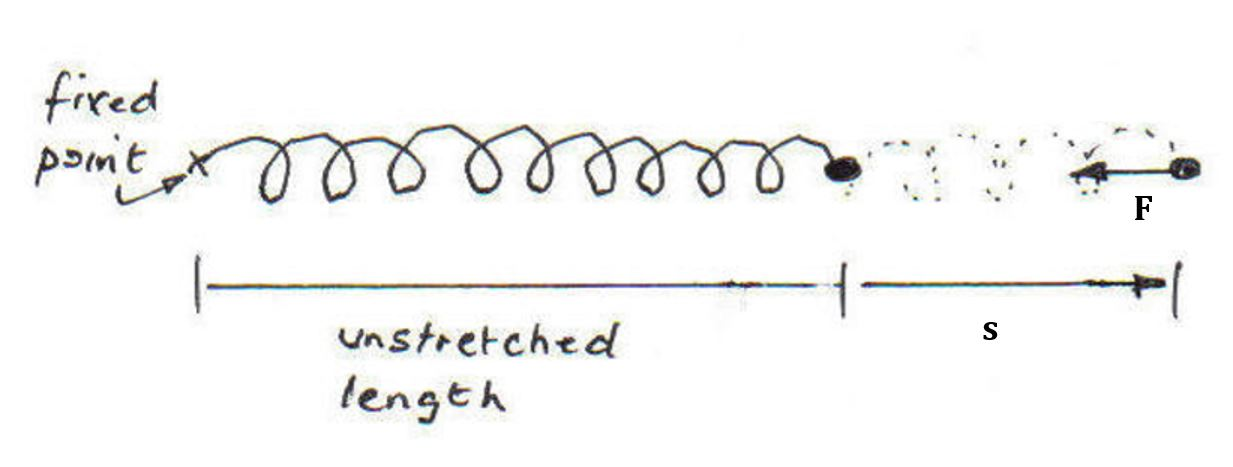
\includegraphics[scale=0.5]{notes/images/SHO.JPG}
    \caption{A simple harmonic oscillator}
    \label{fig:sho}
\end{figure}
\FloatBarrier

The so-called \textbf{restoring force}, a force that acts in the opposite direction to the displacement from the equilibrium position, is given by Hooke's Law (provided the spring obeys Hooke's law); if the Hooke's law is obeyed then the device is called a \textbf{simple harmonic oscillator} (often abbreviated to \textit{sho}) and the motion of the device is known as \textbf{simple harmonic motion} (abbreviated to \textit{shm}). Since we're only considering simple harmonic oscillators, the restoring force is $\vec{F} = -k \vec{s}$. So the equation of motion is
\begin{equation}
    \label{eq:shm-diff-eq-1}
    \vec{F} = - k \vec{s} = m \frac{\mathop{\mathrm{d}^2 \vec{s}}}{\mathop{\mathrm{d}t^2}}
\end{equation}
or, 
\begin{equation}
    \label{eq:shm-diff-eq-2}
    \frac{\mathop{\mathrm{d}^2 \vec{s}}}{\mathop{\mathrm{d}t^2}} + \frac{k}{m} \vec{s} = 0
\end{equation}
This is a second order, linear differential equation and can be solved via an auxiliary equation; Firstly, since $\vec{s}$ is in one dimension, we can assume that solutions exist of the form $\vec{s} = \eta \exp(\alpha t)$, where $\eta$ and $\alpha$ are constants.  So we have
\begin{align*}
    \frac{\mathop{\mathrm{d}^2 \vec{s}}}{\mathop{\mathrm{d}t^2}} + \frac{k}{m} \vec{s} &= \eta \alpha^2 \exp (\alpha t) + \eta \frac{k}{m} \exp(\alpha t) \\
    &= \eta \exp (\alpha t) \left(\alpha^2 + \frac{k}{m}\right) = 0
\end{align*}
So our auxiliary equation is 
\begin{equation*}
    \alpha^2 + \frac{k}{m} = 0,
\end{equation*}
giving 
\begin{equation*}
    \alpha = \pm \sqrt{\frac{k}{m}} i,
\end{equation*}
or, writing the \textbf{angular frequency} as $\omega = \sqrt{k / m}$, we have
\begin{equation*}
    \alpha = \pm \omega i
\end{equation*}
So the general solution for $\vec{s}$ is
\begin{equation}
    \vec{s} = A \cos \omega t + B \sin \omega t,
\end{equation}
where $A$ and $B$ are constants of integration of the second-order differential equation in \ref{eq:shm-diff-eq-2}. The solution can also be written in the form
\begin{equation}
    \vec{s} = C \exp \left(i \omega t \right) + D \exp \left( -i \omega t \right),
\end{equation}
where $C$ and $D$ are two arbitrary constants of integration, or as 
\begin{equation}
    \vec{s} = r \sin \left( \omega t + \phi \right).
\end{equation}
with amplitude $r$ and an arbitrary phase angle $\phi$. 

We briefly mentioned angular frequency in the equations above, however let us now formally define it. The \textbf{angular frequency} $\omega$ is defined as the range of change of the phase angle $\phi$; mathematically, we have
\begin{equation}
    \omega = \frac{\mathop{\mathrm{d}\phi}}{\mathop{\mathrm{d}t}}.
\end{equation}
But, this definition provides no physical meaning. Angular frequency (related to angular velocity) is great for systems that rotate or revolve, but our system is oscillating, so we tend to avoid this definition of $\omega$ and define it in terms of coefficients grounded in physical reality (such as frequency).  

A \textbf{periodic system} is one in which the time between repeated events is constant, The time between repeating events in a periodic system is called a \textbf{period}, denoted as $T$. Mathematically, it's the time $t$ per number of events $n$;
\begin{equation}
    T = \frac{t}{n},
\end{equation}
measured in \textbf{seconds} ($s$). \textbf{Frequency} is defined as the rate at which a periodic event occurs, denoted as $f$. Mathematically, it's the number of events $n$ per time $t$;
\begin{equation}
    f = \frac{n}{t},
\end{equation}
measured in \textbf{Hertz} ($Hz$). Note that frequency and period are reciprocals of each other, that is
\begin{equation*}
    f = \frac{1}{T} \hspace{3mm} \iff \hspace{3mm} T = \frac{1}{f}.
\end{equation*}

Angular frequency is \textit{dimensionally} defined as the number of radians per second, whereas frequency is dimensionally defined as the number of events per second, A sequence of repeated events is called a cycle. The sine function has a period of $2 \pi$ and therefore the simple harmonic oscillator repeats itself after it has moved through a single cycle of simple harmonic motion. So we have
\begin{align*}
    \omega = \frac{\phi}{t} &= \frac{2\pi \text{ radian}}{1 \text{ period}} \\
    f = \frac{n}{t} &= \frac{1 \text{ cycle}}{1 \text{ period}}
\end{align*}
Dividing one equation by the other, yields 
\begin{equation*}
    \frac{\omega}{f} = 2 \pi,
\end{equation*}
and thus
\begin{equation}
    \omega = 2\pi f = \frac{2 \pi}{T}.
\end{equation}
So the (preferred) general solution to the simple harmonic oscillator is
\begin{equation}
    \vec{s} = A \sin (2 \pi ft + \phi), 
\end{equation}
where $\vec{s}$ is displacement from the equilibrium position measured in metres, $A$ is amplitude of the simple harmonic motion measured in metres, $f$ is the frequency of the simple harmonic oscillator measured in Hertz and $\phi$ is the phase of the simple harmonic oscillator. Substituting this solution into the original differential equation \ref{eq:shm-diff-eq-1}, we find that
\begin{equation*}
    \frac{k}{m} = 4 \pi^2 f^2,
\end{equation*}
solving for frequency and time period gives
\begin{equation*}
    f = \frac{1}{2\pi} \sqrt{\frac{k}{m}} \hspace{3mm} \text{and} \hspace{3mm} T = 2 \pi \sqrt{\frac{m}{k}}.
\end{equation*}
So angular frequency can be defined in terms of the particle's mass and the spring constant
\begin{equation}
    \omega = \sqrt{\frac{k}{m}}.
\end{equation}
We should also note that the frequency and time period do not affect the amplitude, so a sho oscillating with a large amplitude will have the same frequency and period as an identical sho oscillating with a smaller amplitude.

The velocity of the particle can be found by considering the first time derivative of displacement, so we have
\begin{equation}
    \vec{v} = \frac{\mathop{\mathrm{d}\vec{s}}}{\mathop{\mathrm{d}t}} = \frac{\mathrm{d}}{\mathop{\mathrm{d}t}} (A \sin(2\pi ft + \phi)) = 2 \pi f A \cos(2\pi f t + \phi).
\end{equation}
Applying $\omega = 2\pi f$ and $\sin^2 \theta + \cos^2 \theta \equiv 1$ to the equation above yields an equation for speed $v$;
\begin{equation*}
    v = \pm \omega \sqrt{A^2 - \| \vec{s} \|^2},
\end{equation*}
For acceleration, we could take the derivative of velocity with respect to time, however, if we consider the differential equation in \ref{eq:shm-diff-eq-1}, we quickly see that
\begin{equation*}
    m \vec{a} = - k \vec{s},
\end{equation*}
so 
\begin{equation}
    \vec{a} = - \omega^2 \vec{s} = -\omega^2 A \sin(2 \pi f t + \phi).
\end{equation}

\subsection{Potential and Kinetic Energy in Simple Harmonic Motion}

We now consider the variations of the potential energy and kinetic energy of the particle as it undergoes simple harmonic motion. The force $\vec{F} = - k \vec{s}$ is a conservative force so the elastic potential energy $E_p$ is 
\begin{equation}
    E_p = \frac{1}{2} k \| \vec{s} \|^2 + E_{p, 0},
\end{equation}
where $E_{p,0}$ denotes the potential energy at the equilibrium position $\vec{s} = 0$. We can choose $E_{p, 0} = 0$ $J$ and so the potential energy is given by
\begin{equation}
    E_p = \frac{1}{2} k \| \vec{s} \|^2 = \frac{1}{2} k A^2 \sin^2 (\omega t + \phi) = \frac{1}{2} k A^2 \sin^2 (2 \pi f t + \phi)
\end{equation}
The kinetic energy $E_k$ or the particle is given by
\begin{equation}
    E_k = \frac{1}{2} m \| \vec{v} \|^2 = \frac{1}{2}m \omega^2 A^2 \cos^2(\omega t + \phi) = 2 \pi^2 m f^2 A^2 \cos^2 (2 \pi f t + \phi)
\end{equation}

\noindent The total energy of the system $E$ is $E = E_k + E_p$, so
\begin{equation}
    E = \frac{1}{2} m \omega^2 A^2 \cos^2 (\omega t + \phi) + \frac{1}{2} k A^2 \sin^2 (\omega t + \phi),
\end{equation}
but $\omega^2 = k / m$, so
\begin{align*}
    E &= \frac{1}{2} m A^2 \frac{k}{m} A^2 \cos^2 (\omega t + \phi) + \frac{1}{2} k A^2 \sin^2 (\omega t + \phi) \\
    &= \frac{1}{2} k A^2 \left[\sin^2(\omega t + \phi) + \cos^2(\omega t + \phi)\right],
\end{align*}
hence, 
\begin{equation}
    E = E_k + E_p = \frac{1}{2}kA^2. 
\end{equation}

\subsection{Damped Oscillations}

In all \textbf{real} mechanical oscillators there is some form of \textbf{damping} (or resistive force acting on the system). The damping force opposes the motion of the particle. Consider a damping force that is proportional to velocity of the particle, i.e. $\vec{F}_f = -b \vec{v}$ with a positive constant $b$. Suppose the velocity is positive (parallel to positive $\vec{s}$), then the damping force is in the opposite direction. See figure ??.

In general, a particle in simple harmonic motion has the following equation of motion
\begin{equation}
    \frac{\mathop{\mathrm{d}^2\vec{s}}}{\mathop{\mathrm{d}t^2}} = - \omega^2 \vec{s} \text{ or }
    \frac{\mathop{\mathrm{d}^2\vec{s}}}{\mathop{\mathrm{d}t^2}} + \omega^2 \vec{s} = 0.
\end{equation}
However in the case of damped harmonic motion, the equation of motion is
\begin{equation}
    \frac{\mathop{\mathrm{d}^2\vec{s}}}{\mathop{\mathrm{d}t^2}} + \frac{b}{m} \frac{\mathop{\mathrm{d}\vec{s}}}{\mathop{\mathrm{d}t} }+ \omega^2 \vec{s} = 0,
\end{equation}
or more commonly we let $\lambda = b/m$, so we have

\begin{equation}
    \frac{\mathop{\mathrm{d}^2\vec{s}}}{\mathop{\mathrm{d}t^2}} + \lambda \frac{\mathop{\mathrm{d}\vec{s}}}{\mathop{\mathrm{d}t} }+ \omega^2 \vec{s} = 0,
\end{equation}
This is a second-order, linear, homogeneous differential equation with constant coefficients $\lambda$ and $\omega^2$. So the general solution is dependent on the discriminant of the auxiliary equation
\begin{equation}
    q^2 + \lambda q + \omega^2 = 0.
\end{equation}
So we have three cases:
\begin{itemize}
    \item When $\lambda^2 - 4 \omega^2 > 0$, then the auxiliary equation has two distinct real roots and the general solution is 
    \begin{equation}
        \vec{s} = c_1 \exp(q_1 t) + c_2 \exp(q_2 t).
    \end{equation}
    This is classed as heavy damping.
    \item When $\lambda^2 - 4 \omega^2 = 0$, then the auxiliary equation has a repeated real root and the general solution is
    \begin{equation}
        \vec{s} = (c_1 t + c_2) \exp(q_1 t).
    \end{equation}
    This is classed as critical damping. 
    \item When $\lambda^2 - 4 \omega^2 < 0$, the the auxiliary equation has two distinct complex roots and the general solution is
    \begin{equation}
        \vec{s} = \exp\left(-\frac{\lambda}{2}t\right) \left[c_1 \sin \left(\frac{\alpha}{2}t\right) + c_2 \cos \left(\frac{\alpha}{2}t\right)\right]   ,
    \end{equation}
    where $\alpha^2 = 4 \omega^2 - \lambda^2$. This is classed a light damping.
\end{itemize}

\begin{figure}[h!]
    \centering
    \begin{tikzpicture}
        \draw[->] (-1,0)--(15,0) node [above left]  {$t$};
        \draw[->] (0,-4)--(0,4) node [below right]  {$\vec{s}$};
        \draw[scale=2,domain=0:7,smooth,variable=\x,blue, thick] plot ({\x}, {1.5 * exp(-1 * \x) - 0.5 * exp(-3 * \x))});
        \draw[scale=2,domain=0:7,smooth,variable=\x,red, thick] plot ({\x}, {exp(-2 * \x) * (1 + 2 * \x)});
        \draw[scale=2,domain=0:7,smooth,variable=\x,purple, thick,samples=300] plot ({\x}, {exp(-0.3 * \x) * (cos(1.5 *  deg(\x)))});
        \node[text=blue] at (13,3) {Heavy damping};
        \node[text=red] at (13.1,2.2) {Critical damping};
        \node[text=purple, ] at (12.95,1.4) {Light damping};
    \end{tikzpicture}
\end{figure}
\FloatBarrier

\subsection{Resonance}

In the absence of damping, i.e when $\lambda = 0$ or when the oscillator is said to be in \textbf{free oscillation}, the natural angular frequency of oscillation, denoted by $\omega_0$ is $\sqrt{k/m}$; similarly, the natural frequency of the oscillator denoted $f_0$ is $\omega_0/2\pi$. 

A oscillator is said to be in \textbf{forced oscillation} if there is a periodic driver force applied to the oscillator. In this case oscillator will oscillate at the frequency of the driving force, known as the \textbf{driving frequency}. 

If the driving frequency is equal to the natural frequency of the oscillator, then the oscillator will \textbf{resonate}. When the oscillator resonates, the amplitude of the oscillation increases dramatically. If the system is not damped, the amplitude will increase to the point at which the oscillator breaks / failed (i.e the glass breaks in the context of an opera singer breaking a glass with their voice). Figure \ref{fig:resonance} shows the effect of damping on forced oscillator. 

\begin{figure}[h!]
    \centering
    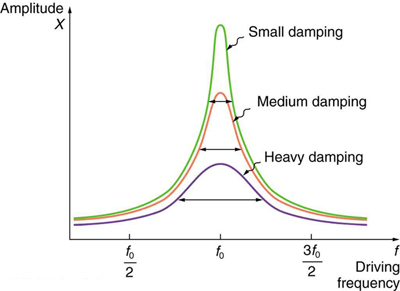
\includegraphics[scale=1.2]{notes/images/Resonance.JPG}
    \caption{Damping on a forced oscillator}
    \label{fig:resonance}
\end{figure}
\FloatBarrier


The greatest possible transfer of energy from the driver to the forced oscillator occurs at the natural frequency, hence the amplitude of the oscillator is maximum at the natural frequency. 

\subsubsection*{Examples of resonance}
\begin{itemize}
    \item \textbf{Clocks} : Clocks can keep time using the resonance of a pendulum or a quartz crystal.
    \item \textbf{Musical Instruments} : Instruments resonate to produce louder notes. 
    \item \textbf{Magnetic Resonance Imaging} : MRI uses resonance effects of hydrogen nuclei to produce diagnostic scans of the inside of our bodies. 
\end{itemize}

\section{Fluids}

\subsection{Density}

The density of a substance is it's mass per unit of volume or the ratio of mass to volume. It is a scalar quantity used to measure the substance's ``compactness''. 

\begin{definition}{(\textbf{Density})}
\textit{The density $\rho$, or the volumetric mass density, of a substance is its mass per unit of volume. Mathematically, density is defined as mass $m$ divided by volume $V$:}
\begin{equation}
    \rho = \frac{m}{V}.
\end{equation}
\textit{measured in \textbf{kilogram per cubic metres} ($kgm^{-3}$).}
\end{definition}

In A2 Physics we are required to know methods for determining density, including regular, non regular objects and fluids (specifically liquids). A regular object has faces which are standard polygons.Non regular objects are therefore those which do not have standard polygons for faces. To determine the density of an object, it's mass and volume must be recorded. The mass is normally measured with a set of digital scales or balances. We now consider the volume of regular, non regular objects and fluids;
\begin{itemize}
    \item \textbf{Fluids}: The volume of a fluid can be determined using a measuring cylinder. 
    \item \textbf{Regular objects}: The volume of a regular object can be determined using calculations based on the geometry of the object. Necessary measurements for such a calculation can be recorded using a ruler, digital calipers or micrometer. 
    \item \textbf{Non regular objects}: The volume of a non regular object can be determined using the \textit{displacement method}, which requires a measuring cylinder and a known amount of liquid (preferably water). Record the initial volume of the liquid $V_0$ in the measuring cylinder. Submerge the object in the liquid and record the new volume of the liquid $V_1$. The volume of the object $V$ can be calculated using the difference of the two recorded volumes, that is
    \begin{equation*}
        V = V_1 - V_0.
    \end{equation*}
\end{itemize} 
We can then calculate the density of the object / fluid using the equation 
\begin{equation*}
    \rho = \frac{m}{V},
\end{equation*}
where $m$ is the recorded mass and $V$ is the recorded / calculated volume. 

\subsection{Pressure}
\label{subsection:pressure}

\begin{definition}{(\textbf{Pressure})}
\textit{Pressure is the amount of force applied \textit{perpendicular} to the surface of an object per unit area over which that force is distributed (i.e. acting). Mathematically; the pressure $p$ of an object is defined as the ratio between the magnitude of the normal force $\| \vec{F}_n \|$ and the area of the surface on contact $A$, that is}
\begin{equation}
    p = \frac{\| \vec{F}_n \|}{A},
\end{equation}
\textit{measured in \textbf{pascals} (Pa).}
\end{definition}

\begin{definition}{(\textbf{Pascals})}
\textit{The SI unit for pressure, the pascal (Pa), is equal to one newton per square metre, thus}
\begin{equation*}
    [Pa] = [Nm^{-2}] = [kgm^{-1}s^{-2}].
\end{equation*}
\end{definition}

The pascal is also a unit of stress and the topics of pressure and stress are connected, however, we will discuss that in a later section. 

\subsection{Liquid Pressure}

When a person swims under the water, water pressure is felt acting on the person (specifically their eardrums). The deeper that person swims, the greater the pressure (due to the weight of the water above them). This is an example of a liquid exerting pressure on a solid.

Liquids exert pressure on solids, since the surfaces of the solids are bombarded by the liquids molecules, thus exerting a force on the surface of the solid. Liquid pressure is dependent of the depth (see introduction). In a similar fashion, it also depends on the density of the liquid. If someone was submerged in a liquid more dense than water, the pressure would be greater, thus we say that depth, density and liquid pressure are directly proportionate. 

\begin{theorem}
\textit{The pressure due to a liquid in liquid columns of constant density or at a depth within is given by the following relationship}
\begin{equation}
    p = \rho \| \vec{g} \| h,
\end{equation}
\textit{where $p$ is liquid pressure, $\| \vec{g} \|$ is the magnitude of acceleration due to gravity, $\rho$ is the density of the liquid and $h$ is the height of the liquid column or depth within a substance.}
\begin{proof}
\textit{Consider an area $A$ at the bottom of a vessel of liquid of height $h$. The weight of the column of liquid directly above this area $\vec{W}$ produces pressure. From this we have}
\begin{equation*}
    \vec{W} = m\vec{g} \textit{ and } \rho = \frac{m}{V} \textit{ and } V = Ah,
\end{equation*}
\textit{where $m$ is the mass and $V$ is the volume of the liquid in the vessel. Combining these equations gives us}
\begin{equation*}
    \vec{W} = A h \rho \vec{g}. 
\end{equation*}
\textit{The we have}
\begin{equation*}
    p = \frac{\| \vec{W} \|}{A} = \frac{Ah\rho \| \vec{g} \|}{A}.
\end{equation*}
\textit{With the area in the numerator and the area in the denominator cancelling each other out, we are left with}
\begin{equation*}
    p = \rho \| \vec{g} \| h.
\end{equation*}
\end{proof}
\end{theorem}

\subsection{Buoyancy}

Archimedes was commission by the King of Syracuse to determine if a golden crown was made for him was made of pure gold or a low grade alloy. As the story goes, Archimedes was in his bath, when he immersed himself in the water and felt a bit lighter. He realized, that this buoyant force he was experiencing could be used to determine the quality of the king's crown. 

\begin{theorem}{\textbf{(Archimedes' Principle)}}
\textit{The magnitude of the buoyant force $\vec{B}$ on an object immerse in a fluid is equal to the magnitude of weight of the fluid displaced.}
\begin{proof}
\textit{Consider an immerse prism/cylinder with a cross-sectional area $A$. The buoyant force $\vec{B}$ is the resultant force and can be explained in terms of pressure differences.}
\begin{align*}
    \| \vec{B} \| &= \| \vec{F}_{bottom} \| - \| \vec{F}_{top} \| \\
    &= (p_{bottom} - p_{top}) A \\
    &= (\rho \| \vec{g} \| h_{bottom} - \rho \| \vec{g} \| h_{top}) A \\
    &= (h_{bottom} - h_{top}) \rho \| \vec{g} \| A \\
    &= \Delta h A \rho \| \vec{g} \| \\
    &= \rho \| \vec{g} \| V \\
    &= m_{fluid} \| \vec{g} \| \\
    &= \| \vec{W}_{fluid} \|
\end{align*}
\textit{where $\rho$ is the density of the liquid, $\Delta h$ is the height difference between the bottom and top of the prism/cylinder.}
\end{proof}

An object will sink if the buoyant force is less than the weight of the object. We can determine whether an object will sink or float by considering it's apparent weight $\vec{W}'$ in a one-dimensional model. Let us first define our directions in $\mathbb{R}$. Any force acting upwards will be negative ($-$) and downwards force will be positive ($+$). So the apparent weight of an object immersed in a fluid is given by 
\begin{align*}
    \vec{W}' &= \vec{W} - \vec{B} \\
    &= m_{object} \| \vec{g} \| - m_{fluid} \| \vec{g} \| \\
    &= (\rho_{object} V - \rho_{fluid} V) \| \vec{g} \| \\
    &= (\rho_{object} - \rho_{fluid}) \| \vec{g} \| V 
\end{align*}
So when;
\begin{itemize}
    \item $\rho_{object} > \rho_{fluid}$ the apparent weight is positive and the object sinks 
    \item $\rho_{object} \leq \rho_{fluid}$ the apparent weight is less than or equal to zero and the object floats.
\end{itemize}
So icebergs float as the density of ice is less than the density of water (which is counter-intuitive if we consider the kinetic model, see section \ref{subsection:kinetic-model}). 
\end{theorem}

\subsection{Drag}
\label{subsection:drag}

The force on an object that resists its motion through a fluid is called drag or viscous friction, denoted $\vec{F}_d$. When the fluid is a gas, like air, it is called aerodynamic drag (or more commonly, air resistance). When the fluid is a liquid, like water, it is called hydrodynamic drag. The ``drag'' equation, derived from Bernoulli's equation for the pressure in a fluid, is 
\begin{equation}
    \| \vec{F}_d \| = \frac{1}{2}\rho C_d A \vec{v} \cdot \vec{v},
\end{equation}
where $C_d$ is the so-called coefficient of drag. We won't derive this equation, but let's take the equation apart to consider why these factors affect drag.
\begin{itemize}
    \item Drag increases with the \textit{density} of the fluid $\rho$. More density, means more mass, hence more momentum, which means more resistance to getting out of the way. The two quantities are directly proportional
    \begin{equation*}
        \| \vec{F}_d \| \propto \rho.
    \end{equation*}
    \item Drag increases with area $A$, what we mean by area is the cross sectional area of the object in the direction of motion. From liquid relationship, we know the force acting on an object due to pressure is proportional to the cross-sectional area. We should note that the liquid pressure relationship can be extrapolated for other fluids such as gases. So the two quantities are directly proportional
    \begin{equation*}
        \| \vec{F}_d \| \propto A.
    \end{equation*}
    \item Drag increases with speed $\| \vec{v} \|$. This should be self-evident. However as drag is a complex phenomena, there are situations where drag is proportional to some power of speed such a one, two or $n$. Most commonly we use speed squared, however in a situation described later on we will use a power of one. Recall that speed is the derivative of distance with respect to time. Solving nonlinear differential equations is extremely tedious, so we usually adopt a simpler model of drag than the ``drag equation''. 
    \begin{equation*}
        \| \vec{F}_d \| \propto \| \vec{v} \|^n
    \end{equation*}
\end{itemize}
Combining these factors will produce a similar equation to the ``drag equation''. Although this is not a proof or derivation it allows us to understand why the drag equation is an acceptable model of drag. 

\subsubsection{Terminal Velocity}

Terminal velocity is the highest velocity attainable by an object as it falls through a fluid. Mathematically, it occurs when the drag force $\vec{F}_d$ balances the downwards force of gravity, weight $\vec{W}$. 



Let us now imagine we're parachute jumper (another age old example). We jump of the drop plane and draw our free body diagram as we fall. Initially we have no velocity, there is no aerodynamic drag, we're effectively in free fall with an acceleration due to gravity of magnitude $9.8$ $ms^{-1}$ (See figure \ref{fig:terminal-velocity-1}). 

\begin{figure}[h!]
    \centering
    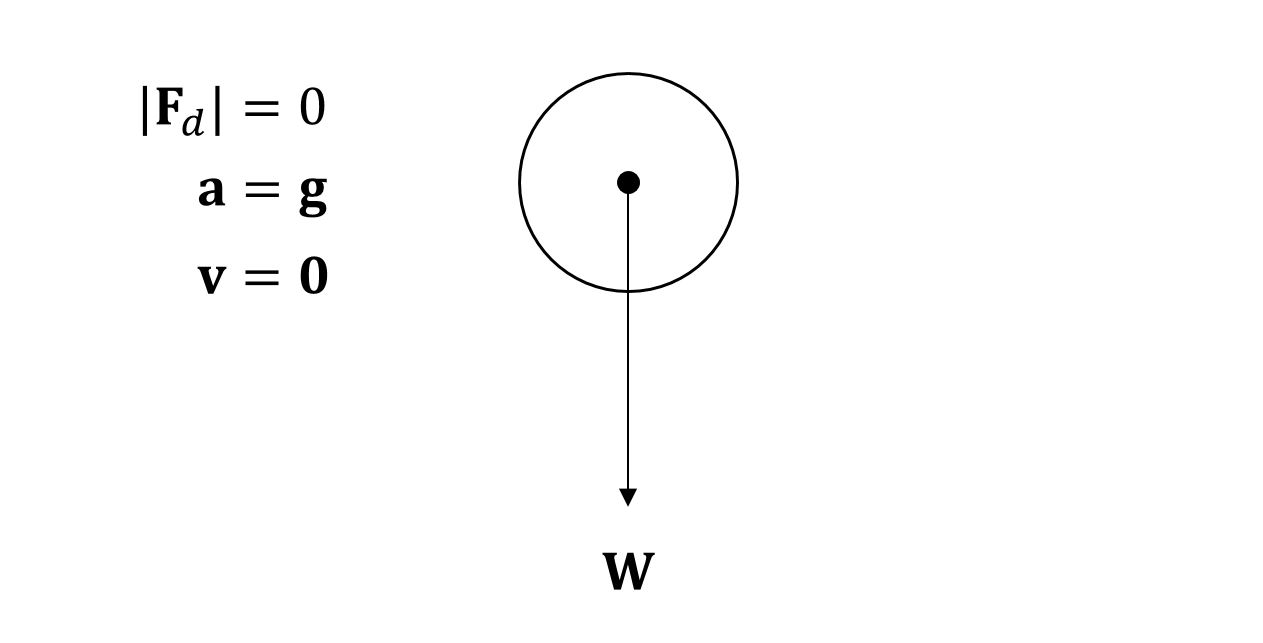
\includegraphics[scale=0.3]{notes/images/Terminal-Velocity-1.JPG}
    \caption{A free body of a sky diver: initially, pre-parachute }
    \label{fig:terminal-velocity-1}
\end{figure}
\FloatBarrier

Now it gets complicated. There is an initial acceleration, therefore an increase in velocity. With an increase in velocity comes an increase in drag and a decrease in our resultant force. This decrease in resultant force reduces acceleration (See figure \ref{fig:terminal-velocity-2}). 
\begin{figure}[h!]
    \centering
    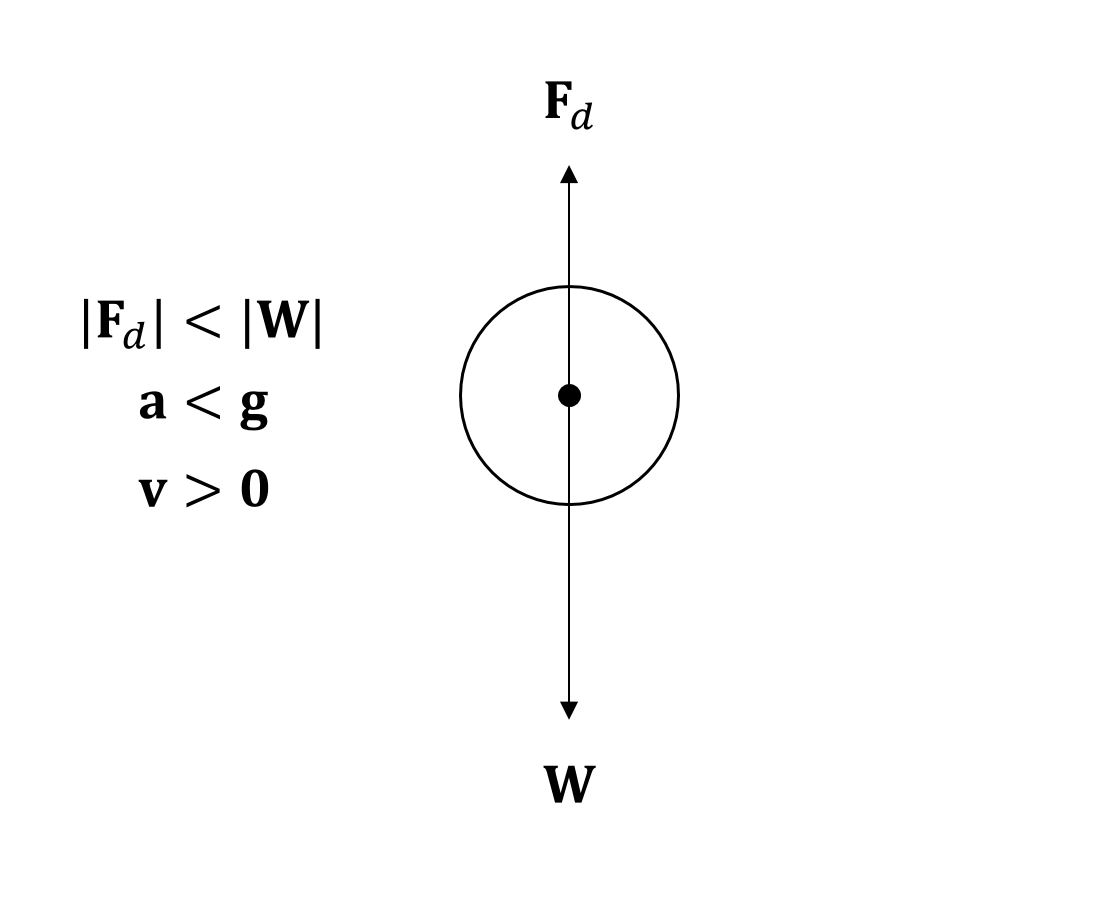
\includegraphics[scale=0.3]{notes/images/Terminal-Velocity-2.JPG}
    \caption{A free body of a sky diver: prior to terminal velocity, pre-parachute }
    \label{fig:terminal-velocity-2}
\end{figure}
\FloatBarrier
Velocity continues to increase, so does drag. As drag increases, acceleration decreases. Eventually we reach a state of equilibrium. We have reached \textit{terminal velocity}. (See figure \ref{fig:terminal-velocity-3})
\begin{figure}[h!]
    \centering
    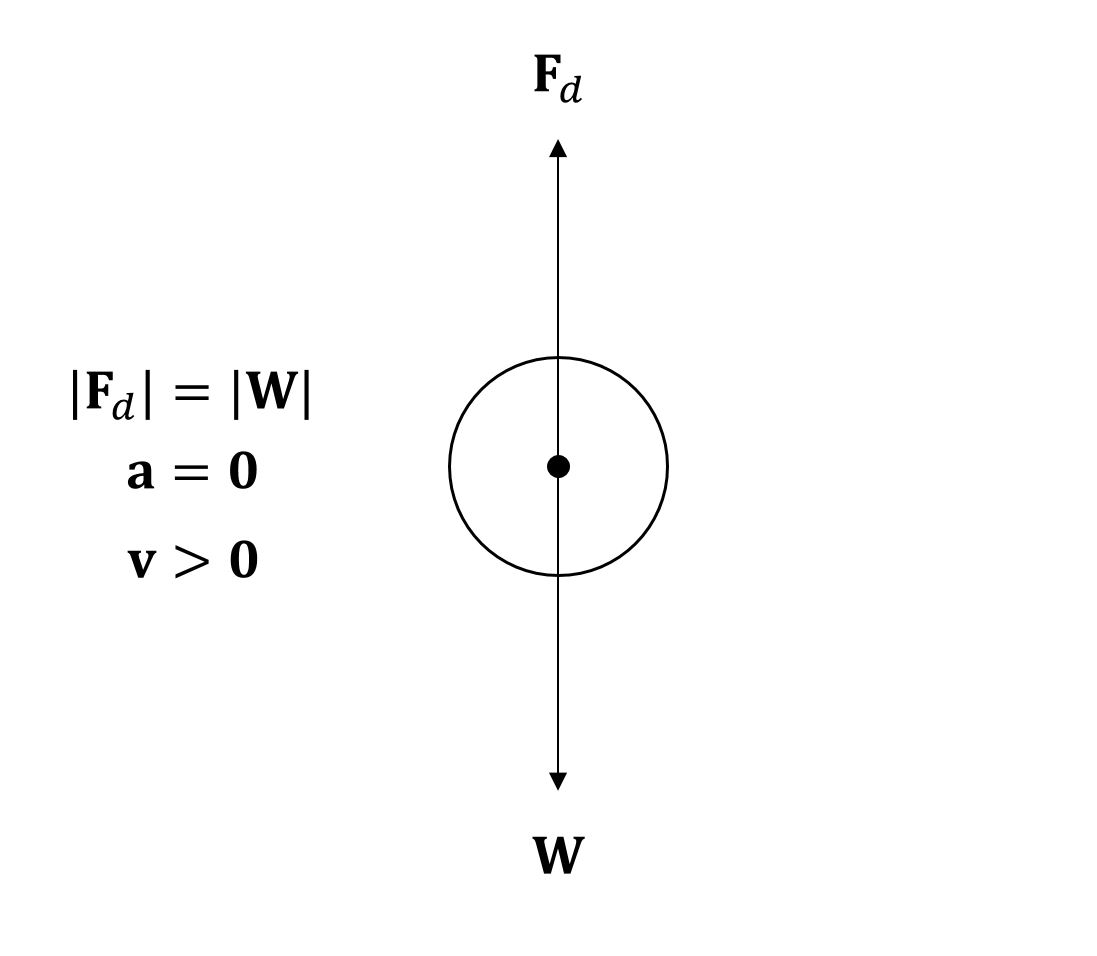
\includegraphics[scale=0.3]{notes/images/Terminal-Velocity-3.JPG}
    \caption{A free body of a sky diver: terminal velocity, pre-parachute }
    \label{fig:terminal-velocity-3}
\end{figure}
\FloatBarrier
We then open our parachute. Opening the chute significantly increases our areas, which increases drag. The upwards drag force is now greater than our weight. The resultant force and acceleration are now directed upwards (deceleration). (See figure \ref{fig:terminal-velocity-4}). 
\begin{figure}[h!]
    \centering
    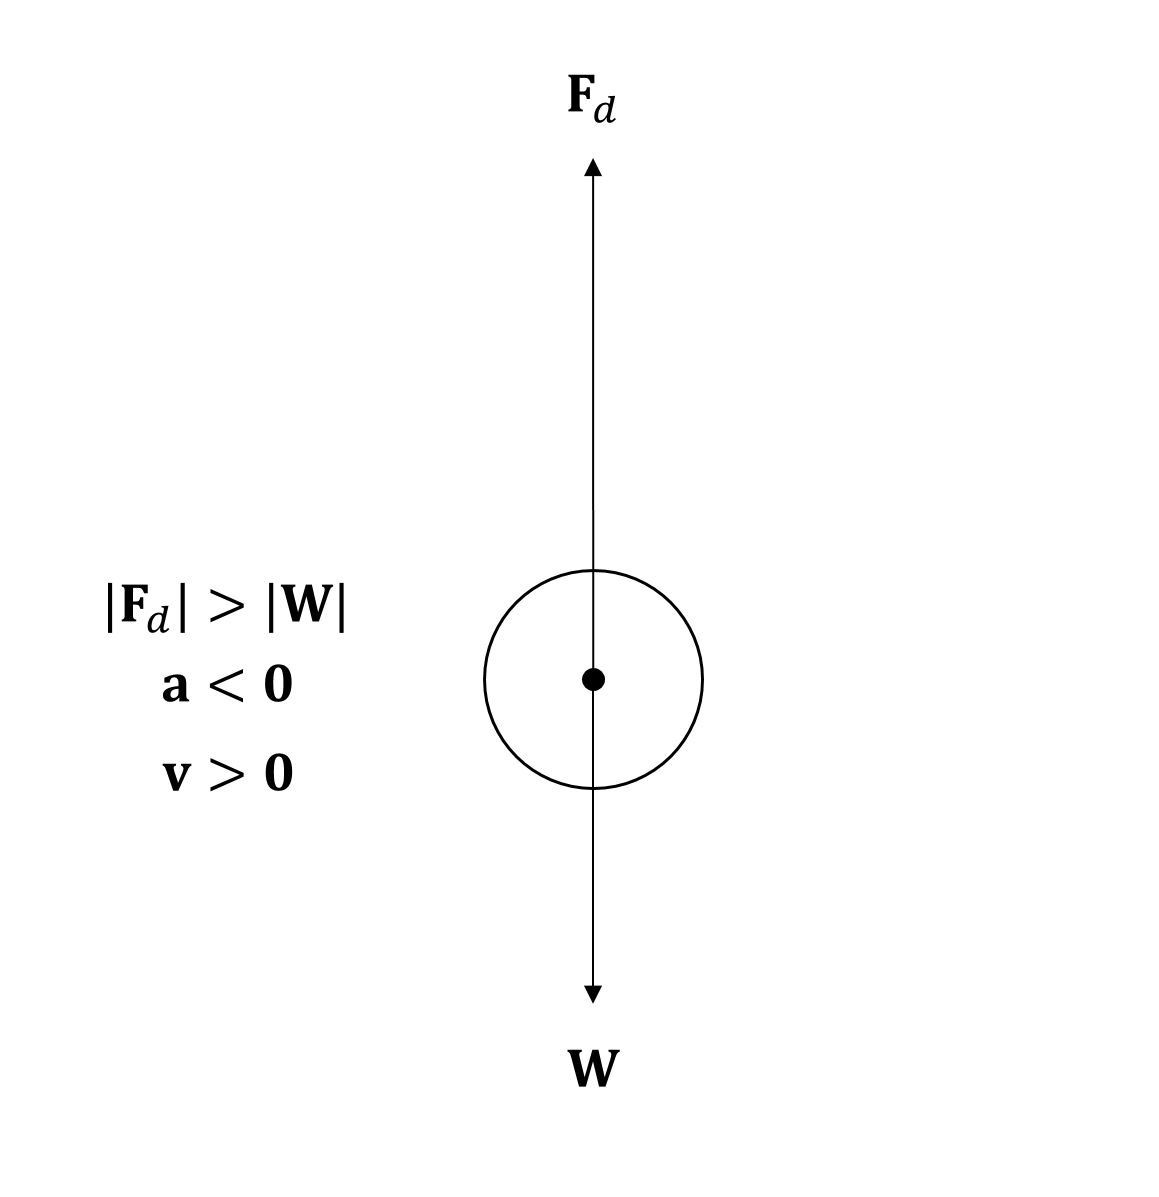
\includegraphics[scale=0.3]{notes/images/Terminal-Velocity-4.JPG}
    \caption{A free body of a sky diver: initially, post-parachute }
    \label{fig:terminal-velocity-4}
\end{figure}
\FloatBarrier
So velocity decreases, so drag decreases. Drag decreases, so the resultant force decreases. Deceleration decreases. (See figure \ref{fig:terminal-velocity-5}).
\begin{figure}[h!]
    \centering
    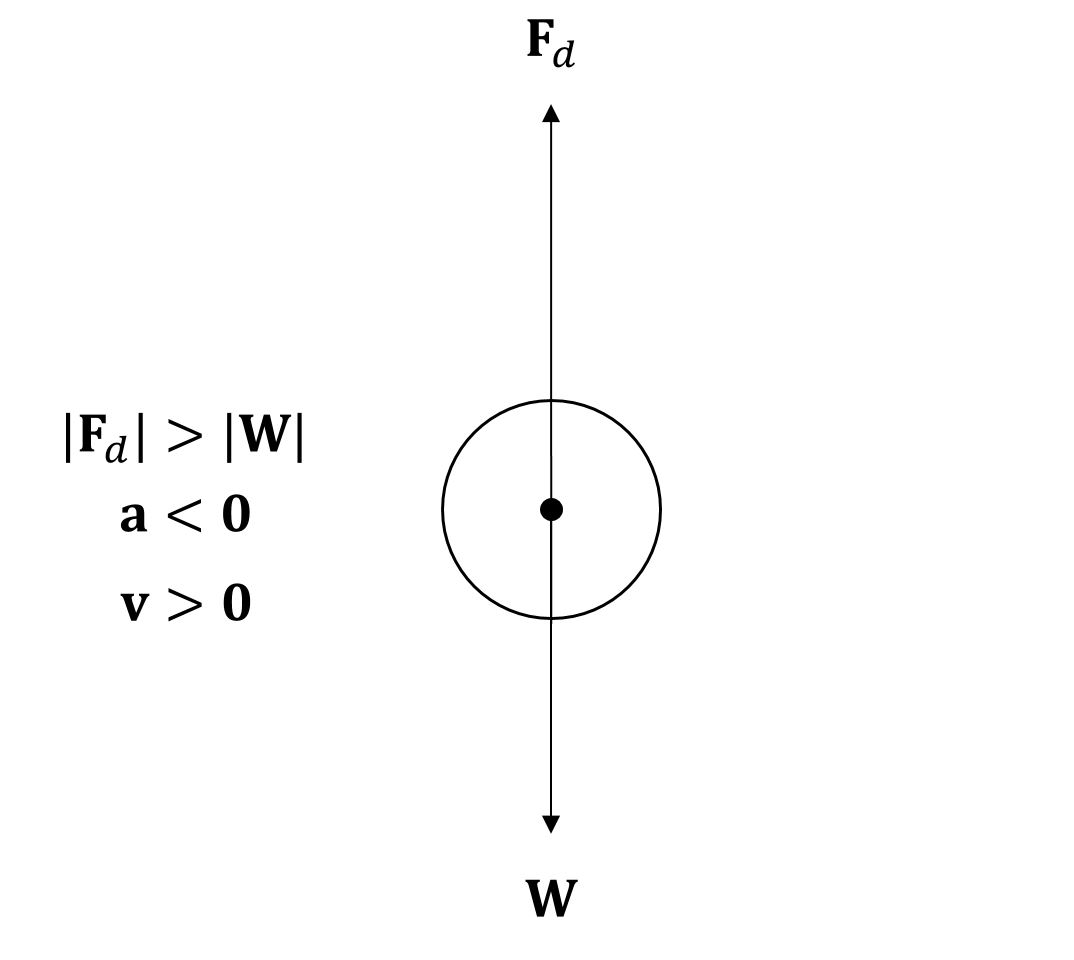
\includegraphics[scale=0.3]{notes/images/Terminal-Velocity-5.JPG}
    \caption{A free body of a sky diver: prior to terminal velocity, post-parachute }
    \label{fig:terminal-velocity-5}
\end{figure}
\FloatBarrier
Eventually we reach another state of equilibrium with a lower velocity. A different terminal velocity.
\begin{figure}[h!]
    \centering
    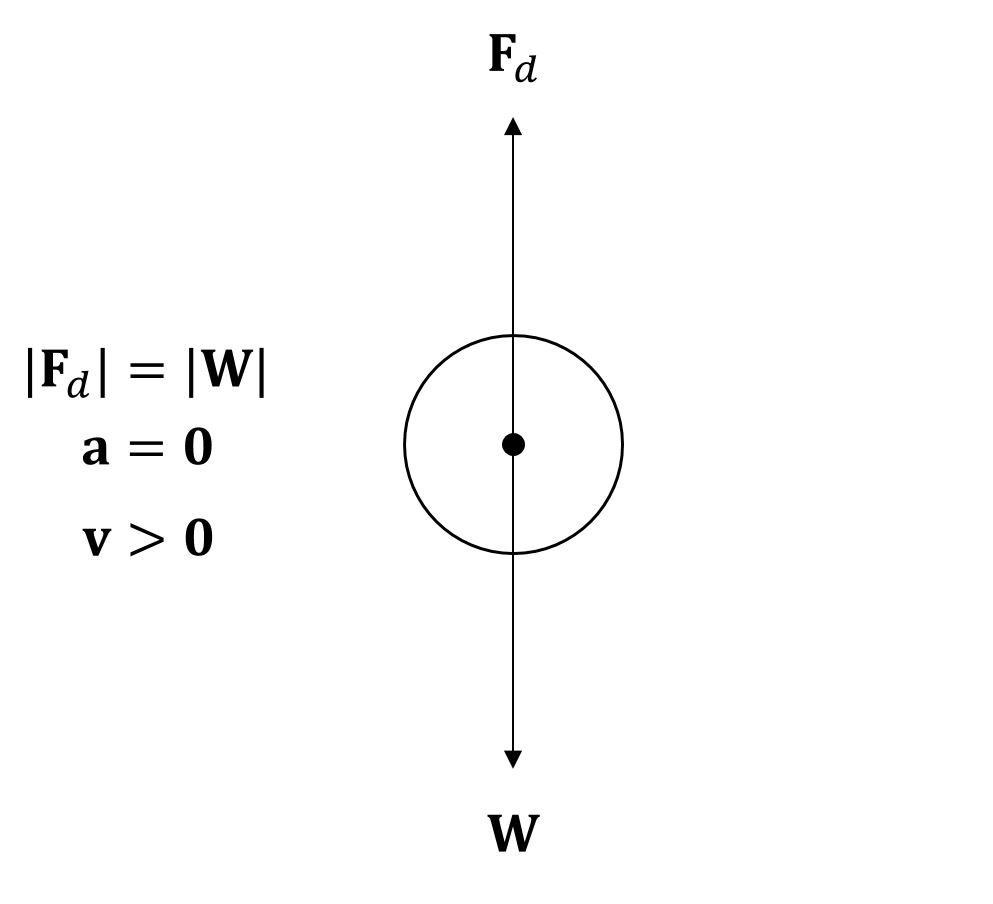
\includegraphics[scale=0.3]{notes/images/Terminal-Velocity-6.JPG}
    \caption{A free body of a sky diver: terminal velocity, post-parachute }
    \label{fig:terminal-velocity-6}
\end{figure}
\FloatBarrier

Having modelled this scenario using dynamics, lets consider an equation of motion for this scenario. As we mentioned earlier, solving non-linear differential equations is tedious, so we will use a simple model for drag.
\begin{equation*}
    \vec{F}_d = -b\vec{v}.
\end{equation*}
This allows us to quickly form an equation of motion,
\begin{equation*}
    m \frac{\mathop{\mathrm{d}\vec{v}}}{\mathop{\mathrm{d}t}} = m \vec{g} - b \vec{v}
\end{equation*}
We can solve this by introducing the integrating factor $e^{bt / m}$ to write the equation as
\begin{equation*}
    \frac{\mathrm{d}}{\mathop{\mathrm{d}t}} (e^{bt/m} \vec{v}) = e^{bt/m} \vec{g}
\end{equation*}
We now integrate, but introduce a vector integration constant $\vec{c}$. We have
\begin{equation*}
    \vec{v} = \frac{m}{t}\vec{g} + \vec{c} e^{-bt/m}
\end{equation*}
We know at time $t = 0$, the velocity is $\vec{v} = \vec{u} = \vec{0}$, so we can use this information to determine the integration constant $\vec{c}$. We get
\begin{equation*}
    \vec{v} = \frac{m}{t}\vec{g}(1 - e^{-bt/m})
\end{equation*}
Now we integrate $\vec{v}$ to determine the displacement as a function of time.  We get another integration constant, $\vec{k}$,
\begin{equation*}
    \vec{s} = \frac{m}{b}\vec{g} \left(t + \frac{m}{b} e^{-bt/m}\right) + \vec{k} 
\end{equation*}
We know, by definition, that at time $t = 0$, we have $\vec{s} = \vec{0}$. Then we have
\begin{equation*}
    \vec{s} = \frac{m}{b}\vec{g} \left(t + \frac{m}{b} e^{-bt/m} - \frac{m}{b}\right) 
\end{equation*}

\section{Examples}

\subsection{Car Stopping Distances}

This section will discuss the factors of car stopping distances, analyzing thinking distance and braking distance separately. This is a specific example of an application of physics to a scenario. Firstly, we shall define stopping distance in terms of thinking and braking distances and then consider the factors that affects them. 

\begin{definition}{(\textbf{Stopping Distance})}
\textit{The stopping distance of a car is defined as the sum of the thinking distance and the braking distance, that is}
\begin{equation*}
    \text{Stopping Distance} = \text{Thinking Distance} + \text{Braking Distance}.
\end{equation*}
\end{definition}

\begin{definition}{(\textbf{Thinking Distance})}
\textit{The thinking distance of a car is the distance travelled by the car during the driver's reaction time (time taken to engage the brakes after seeing the hazard).}
\begin{equation*}
    \text{Thinking Distance} = \| \vec{v} \|t,
\end{equation*}
\textit{where $t$ is the driver's reaction time and $\vec{v}$ is the velocity during that time period.}
\end{definition}
\begin{definition}{(\textbf{Braking Distance})}
\textit{The braking distance of a car is defined as the distance the car travels after the brakes are applied until the car is stationary. Computationally, the braking distance of a car with deceleration $\vec{a}$ and initial velocity of $\vec{u}$ $ms^{-1}$ is}
\begin{equation*}
    \text{Braking Distance} = \frac{\| \vec{u} \|^2}{2\|\vec{a}\|}.
\end{equation*}
\end{definition}

Having formally defined thinking and braking distance, we are now able to consider some of the factors that affects them. We will first consider thinking distance, then braking distance. We notice that thinking distance is dependent on two variables: velocity and reaction time. Which implies to affect thinking distance, we must consider a factor that affects one of these variables. 
\begin{itemize}
    \item The consumption of drugs and/or alcohol will increase the reaction time of the driver $t$, giving rise to an increase in thinking distance; since $t \propto \text{Thinking Distance}$. 
    \item Driver fatigue / tiredness will increase the reaction time of the driver $t$, thus increasing the thinking distance (see relationship above). 
    \item An increase in the velocity of the car during the reaction time period will increase the thinking distance, since $\| \vec{v} \| \propto \text{Thinking Distance}$.
\end{itemize}

Naturally, we can apply the same approach we did to thinking distance to discover the factors that affect braking distance, however, there are some more hidden factors. So lets start by considering the variables, as we did with thinking distance.
\begin{itemize}
    \item An increase in the initial velocity of the car $\| \vec{u} \|$ will the braking distance, since $\| \vec{u} \|^2 \propto \text{Braking Distance}$. 
    \item A decrease in the deceleration of the car $\| \vec{a} \|$ will increase the braking distance, since \\$\text{Braking Distance} \propto \frac{1}{\| \vec{a} \|}$.
\end{itemize}
We now must use concepts such as kinetic energy, work done and friction to explain the two remaining factors that affect braking distance. Firstly we shall consider whether the mass of the car $m$ affects the braking distance. By definition, the kinetic energy of the car, $E_k$, with a mass of $m$ kg and an initial velocity of $\vec{v}$ $ms^{-1}$ is 
\begin{equation*}
    E_k = \frac{1}{2} m \| \vec{v} \|^2.
\end{equation*}
To stop the car, we kinetic energy of the car must be entirely transferred to work done by friction (i.e. friction of the car and friction between of the brakes). So by the work-energy theorem, we can equate these two forms of energies
\begin{align*}
    \frac{1}{2} m \| \vec{v} \|^2 &= \vec{F} \cdot \vec{s} \\
    m &\propto \vec{s}.
\end{align*}

So the braking distance of the car is directly proportional to the mass of the car. Another consideration, is the friction between the car and the road. If the car's tires / brakes are worn or the road is wet/icy it follows that the coefficient of friction $\mu$ will decrease. Given the magnitude frictional force $\vec{F}_f$ is less than or equal to the product of the coefficient of friction and the magnitude normal reaction force $\vec{R}$, that is $\| \vec{F}_f \| \leq \mu \| \vec{R} \|$. So the frictional stopping force between the car and the road is directly proportional to the coefficient of friction. Using a similar application of the work-energy theorem, we have
\begin{equation*}
    \mu \propto \| \vec{F}_f \| \text{ and }  \vec{F}_f  \propto \frac{1}{\vec{s}}.
\end{equation*}
Note that we are working in with a one-dimensional model, so the frictional force is proportional to the magnitude of the friction force. So we conclude that $\mu \propto \frac{1}{\vec{s}}$. Hence the coefficient of friction is inversely proportional to the braking distance. 
    \clearpage
    
    \chapter{Thermal Physics}
    \section{Heat and Temperature}

\subsection{Temperature and Thermal equilibrium}
When two objects are at the same temperature, they are said to be in \textbf{thermal equilibrium}. Thermal energy will flow from a hot object to a cold object until thermal equilibrium is achieved. 

\begin{definition}{(\textbf{Thermal equilibrium})}
\textit{Thermal equilibrium is the state in which there is \textbf{no net flow} of thermal energy between the objects that are involved.}
\end{definition}

\subsection{Laws of Thermodynamics}

\begin{theorem}{(\textbf{Zeroth law})}
\textit{If two systems are both in thermal equilibrium with a third system then they are in thermal equilibrium with each other.}
\end{theorem}

\begin{theorem}{(\textbf{First law})}
\textit{The increase in internal energy of a closed system is }
\begin{equation}
    \Delta U_{system} = \Delta Q - \Delta W
\end{equation}
\textit{where $\Delta U_{system}$ denotes the change in internal energy, $\Delta Q$ denotes the energy entering the system as heat and $\Delta W$ denotes the energy leaving the system as work.}
\end{theorem}
It follows from the first law of thermodynamics that in a thermodynamic cycle of a closed system $\Delta U_{system(\textit{full cycle})}$ is zero
\begin{equation}
    \Delta U_{system(\textit{full cycle})} = 0,
\end{equation}
hence 
\begin{equation}
    Q = Q_{in} - Q_{out} + W_{in} - W_{out} = W.
\end{equation}

\subsection{Temperature Scales}

In order to measure temperature, a scale is required, that includes two fixed points.\\

\noindent \textit{Celsius scale}. The Celsius scale, on the most common temperature scale, uses the freezing point and boiling point of water at atmospheric pressure $(101 \textrm{ kPa})$ are used as two fixed points, $0^{\degree C}$ and $100^{\degree C}$ respectively, with 100 increments between the points. However the Celsius scale can go below $0^{\degree C}$, yet temperature is a scalar quantity, therefore another scale is required.

\begin{notation}
\textit{Temperature in Celsius will be denoted $\theta$.}
\end{notation}

\noindent \textit{The Thermodynamic (Kelvin) scale}. The kelvin scale uses \textit{absolute zero} and the \textit{triple point of water} ($\sim  0.16^{\degree C}$) for two fixed points, $0 \textrm{ K}$ and $273.1 \textrm{ K}$ respectively.

\begin{definition}{(\textbf{Absolute Zero})}
\textit{Absolute zero is the lowest possible temperature, where the internal energy of a substance is at a minimum, therefore $E_k$ of the molecules is $E_k = 0 \textrm{ J}$.}
\end{definition}
\begin{notation}
\textit{Temperature in Kelvin will be denoted $T$.}
\end{notation}
\noindent It follows from the definition of Kelvin and Celsius that
\begin{equation}
    T \approx \theta + 273.
\end{equation}

\begin{experiment}
Using the \textbf{Pressure Law}, $P \propto T$ with a fixed mass of an ideal gas at a constant volume, estimated $0 \textrm{ K}$ in Celsius. 
\end{experiment}

\subsection{The Kinetic Model}
\label{subsection:kinetic-model}

The kinetic model describes the different phases (states) of all substances

\begin{table}[h!]
    \resizebox{17cm}{!}{
        \begin{tabular}{l|l|l|l}
            Phase & Solid & Liquid & Gas  \\
            \hline
            Density ($\rho \textrm{ kg}\mathrm{m^{-3}}$) & $900 \leq \rho \leq 3000$ & $900 \leq \rho \leq 2500$ & $0.1 \leq \rho \leq 1.5$ \\
            Atomic Spacing (m) & $\sim 10^{-10}$ & $\sim 10^{-10}$ & $\sim 10^{-9}$ \\
            Ordering & fixed, structured arrangement & less regular arrangement & random, no arrangement \\
            Motion & vibrating around a fixed point & free to flow / slide past each other & random motion \\
            Strength of electrostatic forces & strong & strong, but not as strong as solids & negligible
        \end{tabular}
    }
\end{table}
\FloatBarrier

\subsection{Internal Energy}

The internal energy of a system changes as a result of heat / energy transfer or work done by or on the system.

\begin{definition}{(\textbf{Internal Energy})}
\textit{The internal energy, $U$, is the sum of all the kinetic energies of the molecules, $E_k$, plus the potential energies, $E_p$, in the chemical bonds holding the atoms and molecules together.}
\begin{equation}
    U = E_k + E_p
\end{equation}
\end{definition}

Increasing the internal energy of a body can be described using the following graph
\begin{figure}[h!]
    \centering
    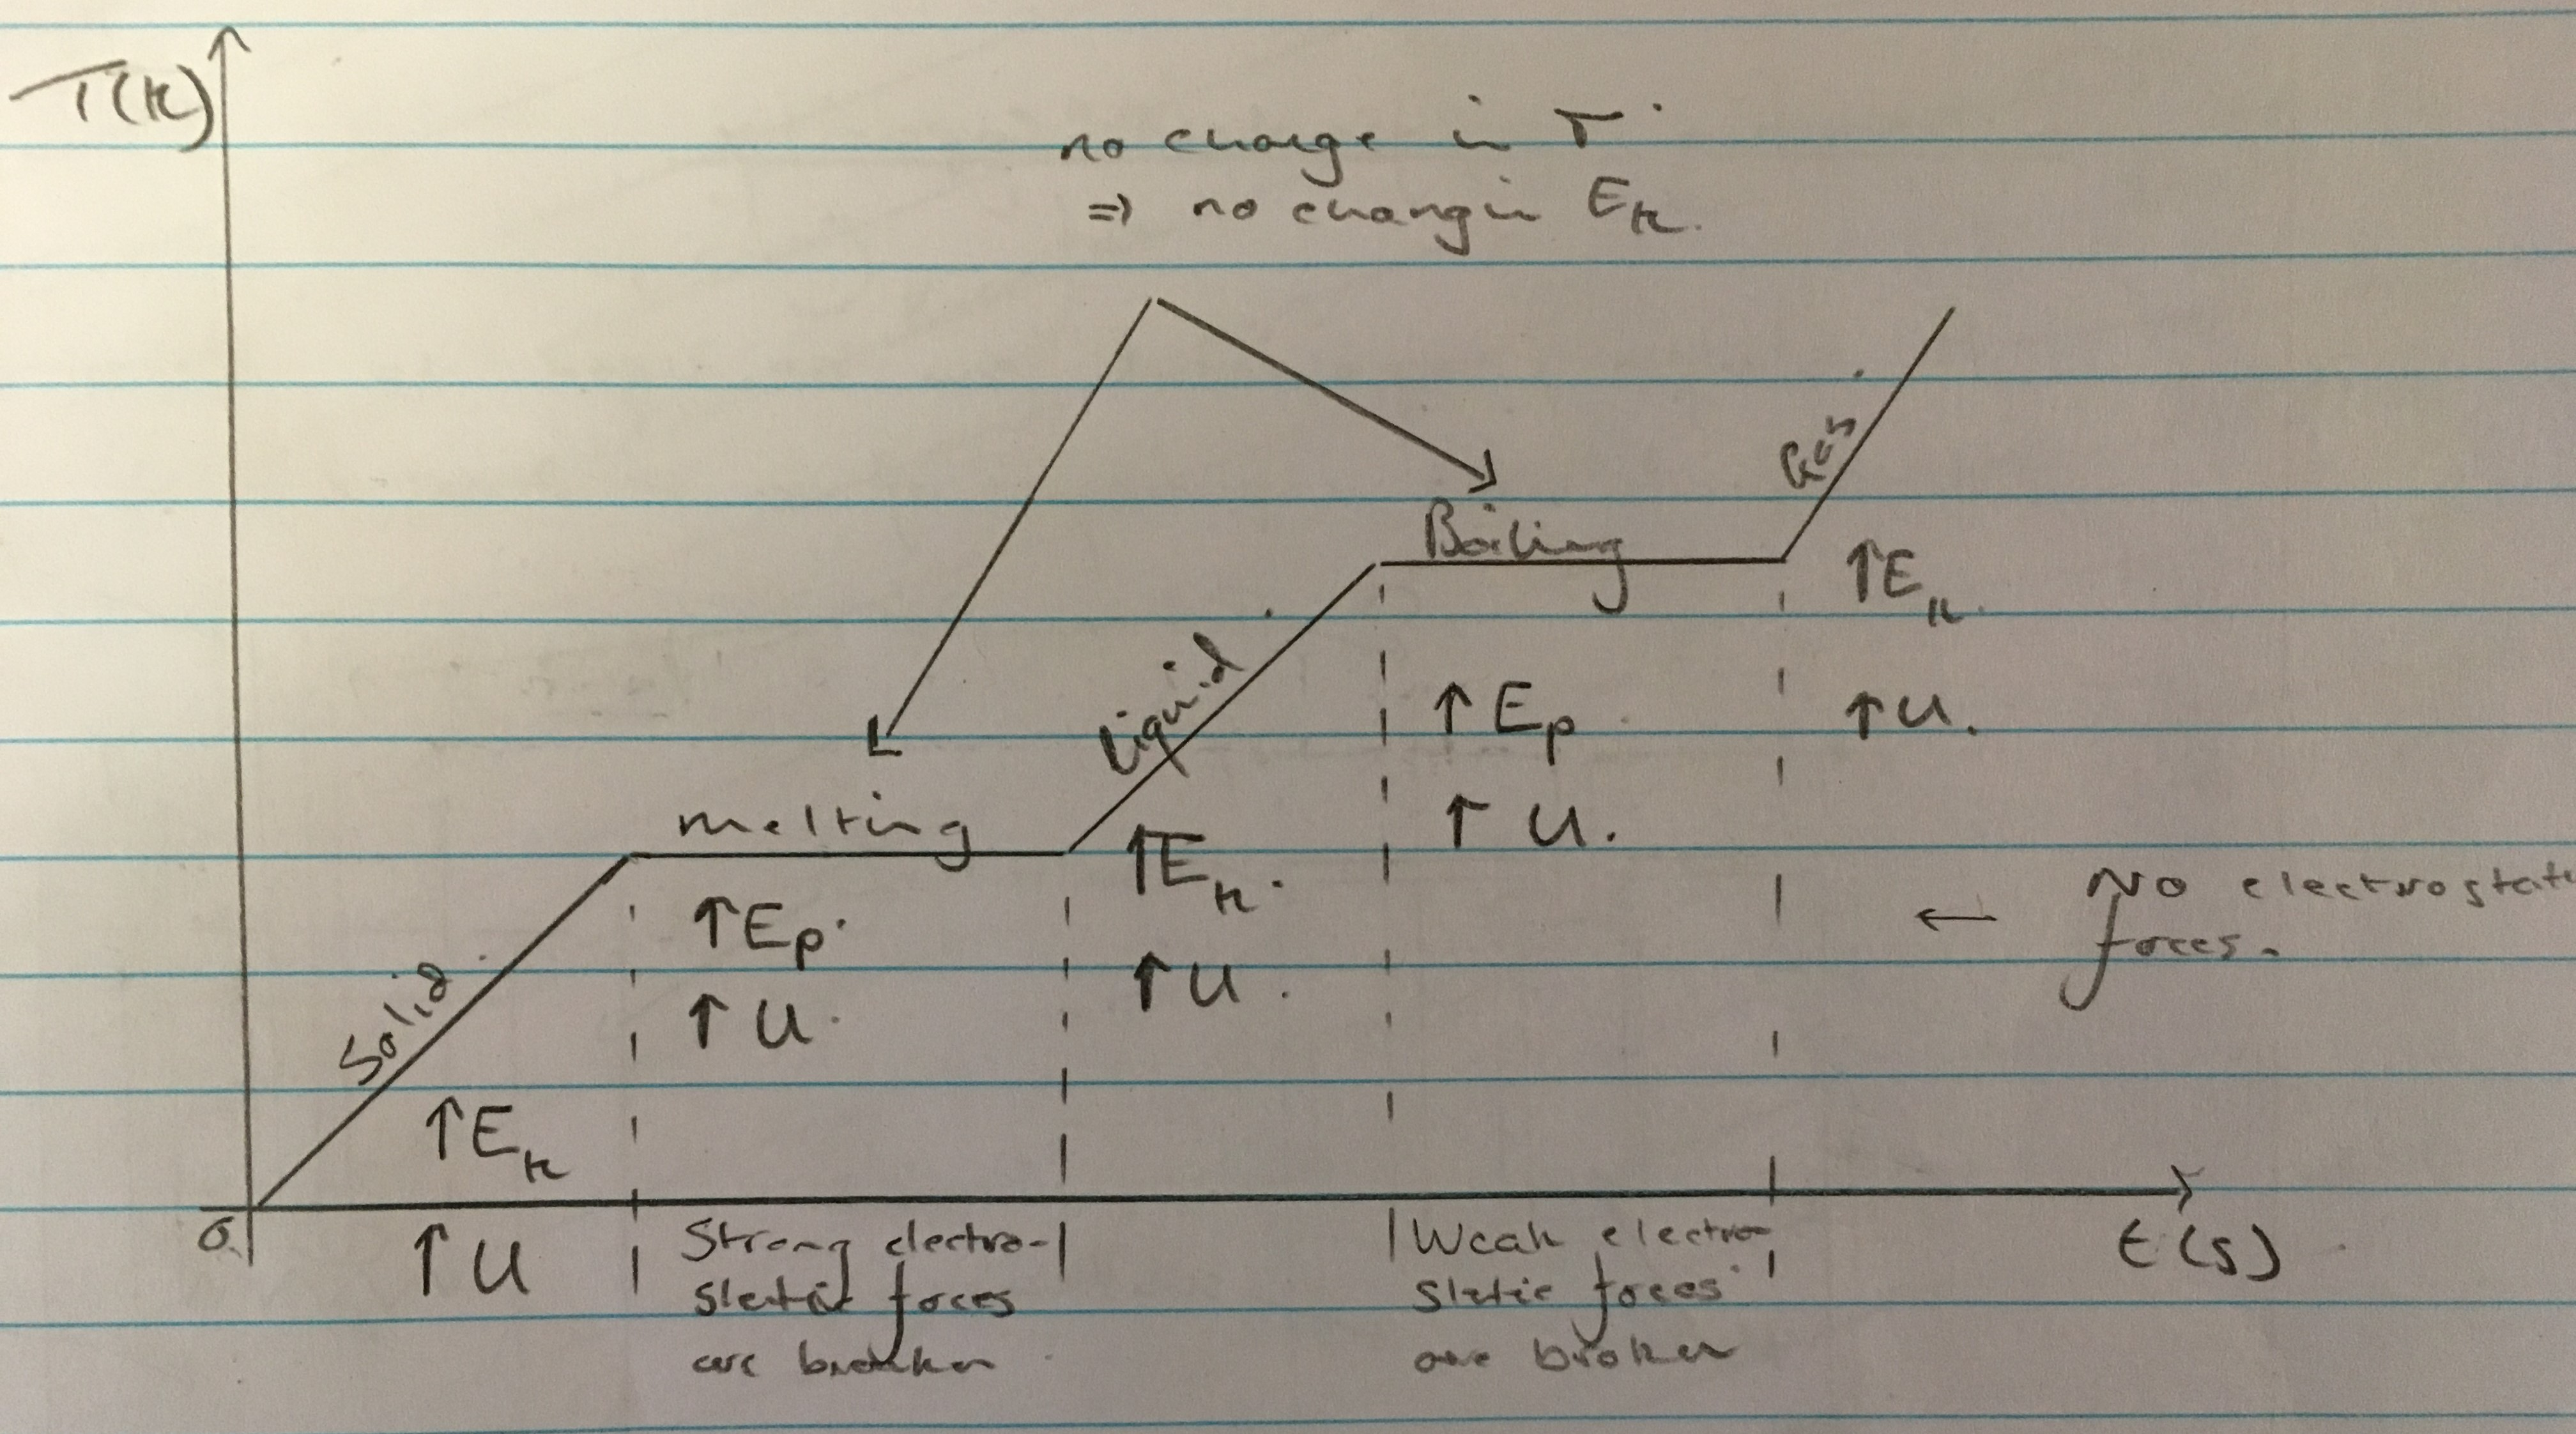
\includegraphics[scale=0.09]{notes/images/Internal-Energy-Graph-Rotated.JPG}
    \caption{Graph showing temperature against time}
\end{figure}
\FloatBarrier


\subsection{Specific Heat Capacity}
\begin{definition}{(\textbf{Specific Heat Capacity})}
\textit{The internal energy required to raise the temperature of a unit mass of a substance by a unit temperature change without change of state.}
\end{definition}

For an object of mass, $m$, with a change in temperature from $T_1$ to $T_2$ of specific heat capacity, $c$, and thermal energy change $\Delta Q$, the following applies,
\begin{equation}
    \label{eq:thermal-energy-change}
    \Delta Q = mc(T_2 - T_2)
\end{equation}
\textbf{NB:} Note that $T_1$ and $T_2$ may be in Kelvin or Celsius.

\subsubsection{Determining Specific Heat Capacity}

A simple experiment can be used to determine the specific heat capacity of a solid or liquid. Let us consider the following apparatus and circuit diagram

\begin{figure}[h!]
    \centering
    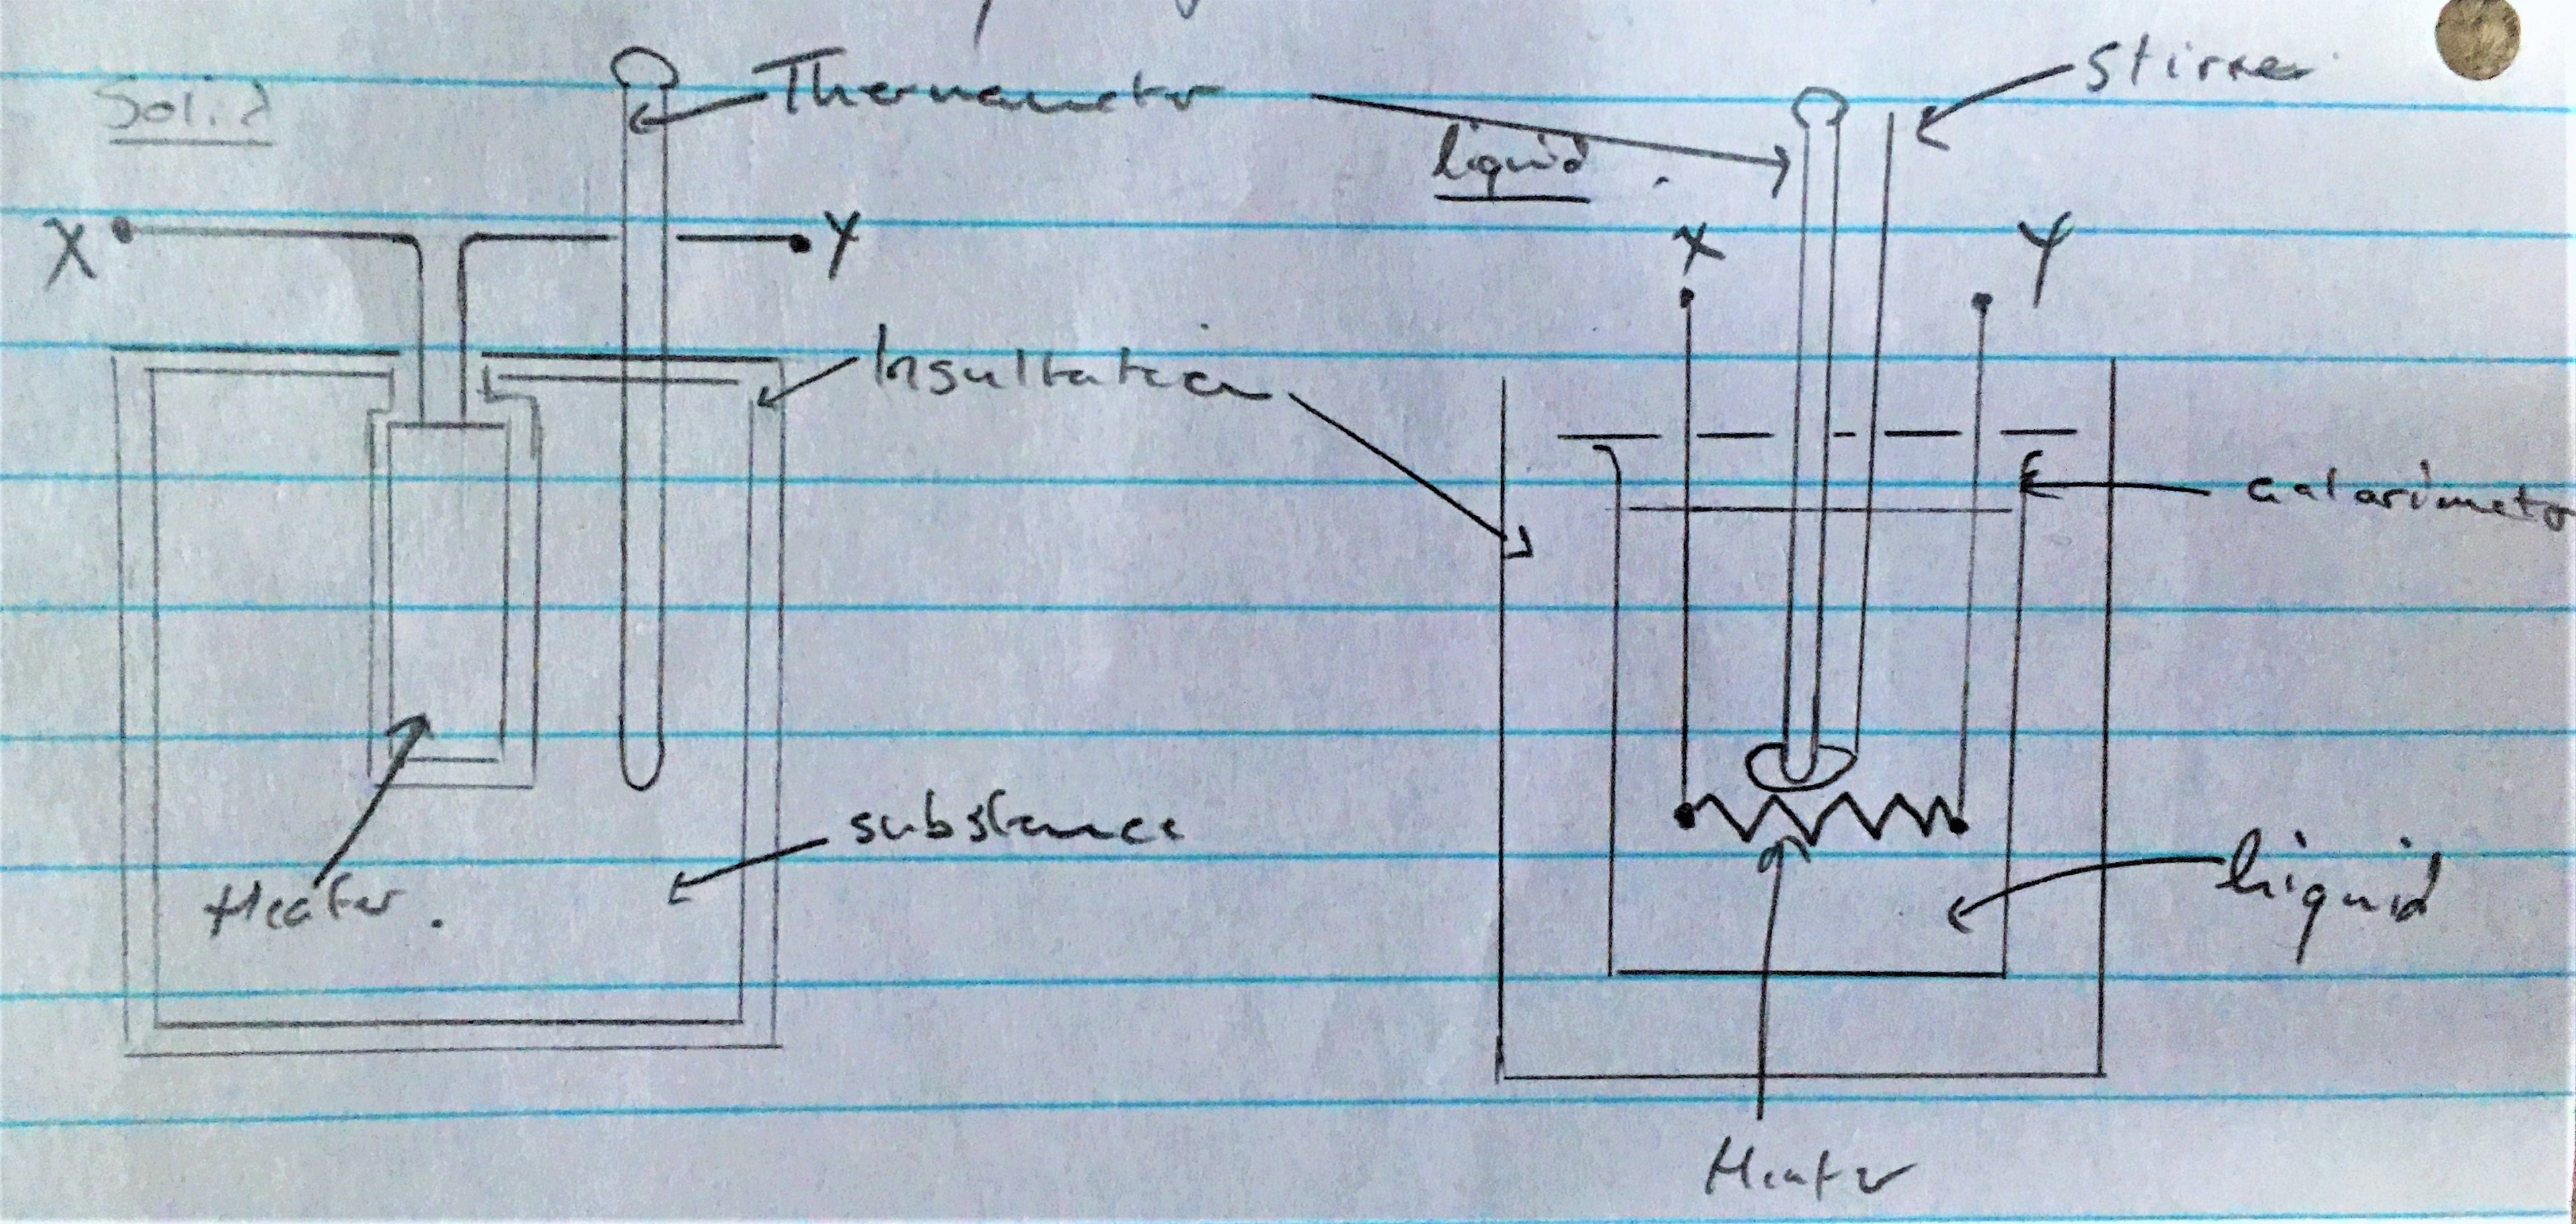
\includegraphics[scale=0.09]{notes/images/Specific-Heat-Capacity.JPG}
    \caption{Solid and liquid apparatus}
\end{figure}
\FloatBarrier

\begin{figure}[h!]
    \centering
    \begin{circuitikz}[scale=0.7]
        \draw (0,0) to [battery, ](0,4) to [ammeter, i_=$I$](4,4) to (4,0) to [short, -*](3,0) node[above] {Y};
        \draw (0,0) to [short, -*](1,0) node[above] {X};
        \draw (3.5,0) to (3.5,-2) to [voltmeter, v=$V$](0.5,-2) to (0.5,0);
    \end{circuitikz}
    \caption{Heating circuit}
\end{figure}
\FloatBarrier

From the definition of work done and electrical power, it follows that the energy inputted into the heater is given by
\begin{equation*}
    \Delta Q = VI\Delta t,
\end{equation*}
where $\Delta t$ is the amount of time required to increase the temperature from $T_1$ to $T_2$. Using equation \ref{eq:thermal-energy-change} we obtain,
\begin{equation*}
    c = \frac{VI \Delta t}{m \Delta T}.
\end{equation*}

However, this is based on the assumption of a closed system which we know not to be true in this scenario. Alternatively, we could repeat this experiment multiple times changing the final temperature $T_2$. The recorded values can then be plotted in a \textit{temperature-time} graph. Drawing a line of best fit can then be used to eliminate some of the uncertainty. For example, we might end up with a graph like this


\begin{figure}[h!]
    \centering
    \begin{tikzpicture}
    \begin{axis}[
        axis lines = left,
        xlabel = $t$,
        ylabel = $T$,
        domain=0:10,
        xmin=0, xmax=10, ymin=0, ymax=15,
        yticklabels=\empty,
        xticklabels=\empty,
        ]
        \addplot[color=red]{0.5*x + 6};
    \end{axis}
    \end{tikzpicture}
\end{figure}
\FloatBarrier

\noindent with a gradient of $k = \frac{\Delta T}{\Delta t}$. If we now consider the equation
\begin{equation*}
    \frac{\Delta Q}{\Delta t} = mc \frac{\Delta T}{\Delta t},
\end{equation*}
and use the definition of power we find that
\begin{equation*}
    P = mc \frac{\Delta T}{\Delta t}.
\end{equation*}
Rearranging this to find $c$, we get
\begin{equation*}
    c = \frac{P}{mk},
\end{equation*}
where $k$ is the gradient of the temperature-time graph and $P$ is the power supplied to the heating circuit. 

\subsection{Specific Latent Heat}

\begin{definition}{(\textbf{Specific Latent Heat})}
\textit{The specific latent heat of a substance $L$ is defined as the thermal energy $Q$ required to change the phase of a substance per unit mass while at a constant temperature; that is}
\begin{equation}
    L = \frac{Q}{m}
\end{equation}
\textit{where $m$ is the mass of the substance and $Q$ is the thermal energy required to change the phase of the substance.}
\end{definition}
\noindent There are two forms of specific latent heat: fusions and vaporization.

\begin{definition}{(\textbf{Specific Latent Heat of Fusion})}
\textit{The specific latent heat of fusion of a substance $L_f$ is defined as the thermal energy $Q$ required to melt a unit mass of the substance at it's melting point; that is}
\begin{equation}
    L_f = \frac{Q}{m}
\end{equation}
\textit{where $m$ is the mass of the substance and $Q$ is the thermal energy required to melt the substance.}
\end{definition}

\begin{definition}{(\textbf{Specific Latent Heat of Vaporization})}
\textit{The specific latent heat of vaporization of a substance $L_v$ is defined as the thermal energy $Q$ required to vaporize a unit mass of the substance at it's boiling point; that is}
\begin{equation}
    L_v = \frac{Q}{m}
\end{equation}
\textit{where $m$ is the mass of the substance and $Q$ is the thermal energy required to vaporize the substance.}
\end{definition}

\subsubsection{Determining Specific Latent Heat}

A simple experiment can be used to determine the specific latent heat of fusion or vaporization of a substance. Let us consider the following apparatus and circuit diagram

\begin{figure}[h!]
    \centering
    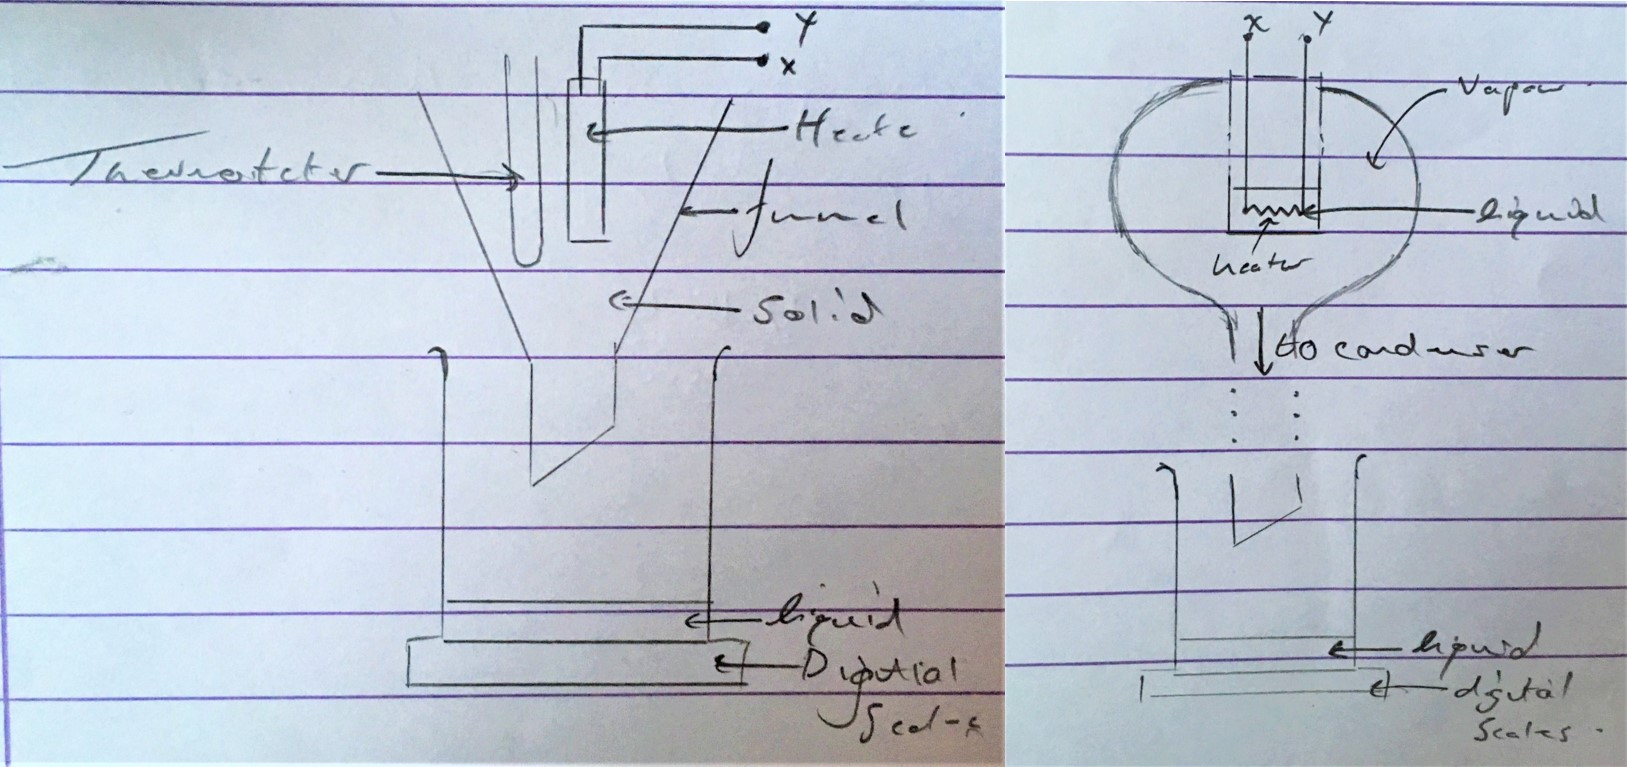
\includegraphics[scale=0.55]{notes/images/Specific-Latent-Heat.JPG}
    \caption{Solid and liquid apparatus}
\end{figure}
\FloatBarrier

\begin{figure}[h!]
    \centering
    \begin{circuitikz}[scale=0.7]
        \draw (0,0) to [battery, ](0,4) to [ammeter, i_=$I$](4,4) to (4,0) to [short, -*](3,0) node[above] {Y};
        \draw (0,0) to [short, -*](1,0) node[above] {X};
        \draw (3.5,0) to (3.5,-2) to [voltmeter, v=$V$](0.5,-2) to (0.5,0);
    \end{circuitikz}
    \caption{Heating circuit}
\end{figure}
\FloatBarrier

From the definition of work done and electrical power, it follows that the energy inputted into the heater is given by
\begin{equation*}
    Q = VI\Delta t,
\end{equation*}
where $\Delta t$ is the amount of time required to produce a change in mass $\Delta m$ in the beaker. Applying the definition of specific latent heat, we find that 
\begin{equation*}
    L = \frac{VI \Delta T}{ \Delta m}
\end{equation*}

We note that in order to obtain an accurate result the thermometer is used to ensure the solid / liquid remains at their melting / boiling points. Otherwise we would need to consider the thermal energy used to increase the temperature.

\section{Ideal Gases}

\subsection{Pressure and Kinetic Theory}

Recall from section \ref{subsection:pressure} that the definition of pressure is:

\begin{definition}{(\textbf{Pressure})}
\textit{The pressure, p, of a gas is defined as the ratio between the magnitude of the normal force $\| \vec{F}_n \|$ and the area of the surface on contact $A$, that is}
\begin{equation}
    p = \frac{\| \vec{F}_n \|}{A},
\end{equation}
\textit{measured in \textbf{pascals} ($Pa$).}
\end{definition}

The \textbf{kinetic theory of gases} is a model used to describe the behaviour of the atoms / molecules in an \textbf{ideal gas}. Real gases have complex behaviour, so in order to keep the model simple a number of assumptions are made, which are as follows:
\begin{itemize}
    \item A gas consists of a large number of particles (refers to gaseous particles only (atoms or molecules)) in random motion.
    \item The internal energy of a gas is entirely kinetic.
    \item Collisions between particles and the walls of the container are perfectly elastic.
    \item The time during collisions is negligible compared to the time between collisions.
    \item Electrostatic forces and gravitational forces are negligible between particles, except during collisions.
    \item The total volume of the atoms/molecules is negligible compared to the volume of gas.
    \item Newton's laws of motion apply to particles. So for example, according to Newton's second law of motion $\vec{F} = \frac{\mathop{\mathrm{d}\vec{p}}}{\mathop{\mathrm{d}t}}$, so the exerted on a particle $\vec{F}_{\textit{on particle}}$ from a collision is given by
    \begin{equation}
        \vec{F}_{\textit{on particle}} = \frac{-m\vec{v} - m \vec{v}}{\Delta t} = - \frac{2m\vec{v}}{\Delta t},
    \end{equation}
    and by Newton's third law of motion, the force exerted by the particle $\vec{F}_{\textit{by particle}}$ during a collision is 
    \begin{equation}
        \vec{F}_{\textit{by particle}} = \frac{2m\vec{v}}{\Delta t},
    \end{equation}
    where $\Delta t$ taken for the change in momentum to occur.
\end{itemize}


\subsection{Gas Laws}

The so-called \textbf{gas laws} state the relationships between pressure, volume and temperature of an ideal gas. The early gas laws are considered to be special cases of the \textit{ideal gas equation}, with one or more variables held constant.

\begin{theorem}{(\textbf{Boyle's Law})}
\textit{The pressure $p$ of a fixed mass of an ideal gas is inversely proportional to it's volume $V$ provided the temperature remains constant.}
\begin{equation}
    p \propto \frac{1}{V} \textit{ or } p_1 V_1 = p_2 V_2.
\end{equation}
\textit{The graph for this inverse relationship is,}
\begin{figure}[h!]
    \centering
    \begin{tikzpicture}
        \begin{axis}[
            axis lines = left,
            xlabel = $V$,
            ylabel = $p$,
            domain=0:10,
            xmin=0, xmax=10, ymin=0, ymax=15,
            yticklabels=\empty,
            xticklabels=\empty,
            samples=300,
        ]
        \addplot[color=red, restrict y to domain=0:15]   {1/(0.1 * x)} node[anchor=east,pos=0.3] {$T_1$};
        \addplot[color=black, restrict y to domain=0:15] {2/(0.1 * x)} node[anchor=east,pos=0.3] {$T_2$};
        \addplot[color=green, restrict y to domain=0:15] {4/(0.1 * x)} node[anchor=east,pos=0.3] {$T_3$};
    \end{axis}
    \end{tikzpicture}
\end{figure}
\FloatBarrier
\noindent \textit{where $T_1 > T_2 > T_3$.}
\end{theorem}

If we consider Boyle's Law, we find that the collisions frequency of the modules of a fixed mass of an ideal gas $f_{collision}$ is directly proportional to the pressure $p$, so we have
\begin{equation}
    f_{collision} \propto p \propto \frac{1}{V}.
\end{equation}

\begin{theorem}{(\textbf{Charles' Law})}
\textit{The volume $V$ of a fixed mass of an ideal gas is proportional to it's temperature $T$ provided the pressure remains constant.}
\begin{equation}
    V \propto T \textit{ or } \frac{V_1}{T_1} = \frac{V_2}{T_2}.
\end{equation}
\textit{The graph for this relationship is,}
\begin{figure}[h!]
    \centering
    \begin{tikzpicture}
        \begin{axis}[
            axis lines = left,
            xlabel = $T$,
            ylabel = $V$,
            domain=0:10,
            xmin=0, xmax=10, ymin=0, ymax=15,
            yticklabels=\empty,
            xticklabels=\empty,
            samples=300,
        ]
        \addplot[color=red, restrict y to domain=0:15]   {2 * x} node[anchor=east,above,pos=0.9] {$N_1$};
        \addplot[color=black, restrict y to domain=0:15] {0.5 * x} node[anchor=east,above,pos=0.9] {$N_2$};
    \end{axis}
    \end{tikzpicture}
\end{figure}
\FloatBarrier
\noindent \textit{where $N_2 > N_1$ and $N$ denotes the number of molecules in the fixed mass of the ideal gas.}
\end{theorem}

\begin{theorem}{(\textbf{The Pressure Law})}
\textit{The pressure $p$ of a fixed mass of an ideal gas is proportional to it's temperature $T$ provided the volume remains constant.}
\begin{equation}
    p \propto T \textit{ or } \frac{p_1}{T_1} = \frac{p_2}{T_2}.
\end{equation}
\textit{The graph for this relationship is,}
\begin{figure}[h!]
    \centering
    \begin{tikzpicture}
        \begin{axis}[
            axis lines = left,
            xlabel = $T$,
            ylabel = $p$,
            domain=0:10,
            xmin=0, xmax=10, ymin=0, ymax=15,
            yticklabels=\empty,
            xticklabels=\empty,
            samples=300,
        ]
        \addplot[color=red, restrict y to domain=0:15]   {2 * x} node[anchor=east,above,pos=0.9] {$N_1$};
        \addplot[color=black, restrict y to domain=0:15] {0.5 * x} node[anchor=east,above,pos=0.9] {$N_2$};
    \end{axis}
    \end{tikzpicture}
\end{figure}
\FloatBarrier
\noindent \textit{where $N_2 > N_1$ and $N$ denotes the number of molecules in the fixed mass of the ideal gas.}
\end{theorem}

\subsection{The Ideal Gas Law}
The \textbf{combined gas equation} is a good approximation of the behaviour of a fixed mass of an ideal gas with no constant variables, however it has several limitations; one being that it only works for a fixed mass of an ideal gas. It is a combination of the empirical Boyle's Law, Charles' Law and the Pressure Law and is written as
\begin{equation}
    \frac{p_1 V_1}{T_1} = \frac{p_2 V_2}{T_2}.
\end{equation}

However, the \textbf{ideal gas law}, also called the \textbf{equation of state} of an ideal gas, is an approximation of the behaviour of many ideal gases under many conditions (i.e. a mass changing system). The equation of state is often written as 
\begin{equation}
    pV = nRT,
\end{equation}
where $p$, $V$, $T$ are the pressure, volume and absolute temperature; $n$ is the number of moles of gas and $R$ is the \textbf{ideal gas constant}. It is the same for all \textit{ideal} gases. The equation of state is frequently written in other forms such as
\begin{equation}
    pV = N k_B T \text{ and } \frac{pV}{T} = nR = N k_B,
\end{equation}
where $k_B$ is the Boltzmann constant. We note the definition of the Boltzmann constant (named after Ludwig Boltzmann) $k_B$ is equivalent to the ideal gas constant $R$ divides by Avogadro's constant $N_A$. Mathematically, we have
\begin{equation}
    \label{eq:boltzmann-constant}
    k_B = \frac{R}{N_A} = \frac{nR}{N} \approx 1.38 \times 10^{-23},
\end{equation}
measured in \textbf{joules per kelvin} ($JK^{-1}$) and where $n$, $N$ denotes the number of moles and molecules, respectively. \\

We will now consider the empirical derivation of the equation of state of an ideal gas with parameters $p_1$, $V_1$, $N_1$ and $T_1$, where $N$ denotes the number of molecules of the ideal gas. Keep in mind, to understand this derivation, one must imagine the gas being altered by one process at a tiime. We first state Boyle's Law, then we have 
\begin{equation*}
    p_1 V_1 = p_2 V_2.    
\end{equation*}
After this process, the gas has the parameters $p_2$, $V_2$, $N_1$ and $T_1$. We now consider a change in temperature and the number of molecules in the gas, we note the relationship $NT = \text{constant}$, so we have 
\begin{equation*}
    N_1 T_1 = N_2 T_2,
\end{equation*} 
so the gas now has the parameters $p_2$, $V_2$, $N_2$ and $T_2$. The change in pressure and the number of particles is given by the following relationship 
\begin{equation*}
    \frac{p_2}{N_2} = \frac{p_3}{N_3},
\end{equation*} 
so we now have the following parameters: $p_3$, $V_2$, $N_3$ and $T_2$. Applying Charles' Law to change the volume and temperature of the gas, we have
\begin{equation*}
    \frac{V_2}{T_2} = \frac{V_3}{T_3}.
\end{equation*}
Using simple algebra on these relations yields the result;
\begin{equation*}
    \frac{p_1 V_1}{N_1 T_1} = \frac{p_2 V_2}{N_2 T_2} \text{ or } \frac{pV}{T} = N k_B.
\end{equation*}
Which is a general case of the combined gas equation we initially stated in this section. Another equivalent result (from equation \ref{eq:boltzmann-constant}) is 
\begin{equation*}
    \frac{pV}{T} = nR,
\end{equation*}
which is known as the \textbf{ideal gas law}.

\subsection{The Maxwell-Boltzmann Distribution}

In Physics, specifically statistical mechanics, the \textbf{Maxwell-Boltzmann distribution} is a probability distribution used for describing the particle speeds in idealized gases. The Mathematics behind the Maxwell-Boltzmann distribution are based on a chi distribution with three degrees of freedom (the components of the velocity vector in the Euclidean space $\mathbf{E}^3$), however since statistics is tedious and boring; we shall go no further than this for understanding why the Maxwell-Boltzmann distribution works. In this course, we shall only consider the mean speeds of particles according to this distribution. The mean speed $\overline{v}$, most probable speed $v_p$ and root-mean-square speed $\sqrt{\overline{v^2}}$ can be obtained from properties of the Maxwell-Boltzmann distribution, however, we will only consider the root-mean-square speed and it's relationship to pressure at a microscopic scale. 

In order to obtain root-mean-square speed of a gas, the velocities of the each particle $\vec{v_1}, \vec{v_2}, \ldots, \vec{v_n}$ are required. We then average the square the components of these velocities in a single dimension to find the mean-square speeds of the gas $\overline{v_{i}^2}$ in the $i^{th}$ dimension, that is
\begin{equation}
    \overline{v_{i}^2} = \frac{1}{n} \sum_{k=1}^n v_{k, i}^2.
\end{equation}
We now must consider the fact that we have a collection of particles moving with a range of speeds in random directions. Any particle may have its velocity $\vec{v}$ resolved into three perpendicular components. We may resolve the mean-square speeds in the same way, so that:
\begin{equation*}
    \overline{v^2} = \overline{v_x^2} + \overline{v_y^2} + \overline{v_z^2}.
\end{equation*}
By definition, the root-mean-square speed $\sqrt{\overline{v^2}}$, sometimes denoted $v_{rms}$, is simply the square root of the mean-square speed, so we have
\begin{equation}
    v_{rms} = \sqrt{\overline{v^2}} = \sqrt{\overline{v_x^2} + \overline{v_y^2} + \overline{v_z^2}} = \sqrt{\frac{1}{n} \sum_{k=1}^n \| \vec{v_k} \|^2}.
\end{equation}
We should also note, that since there are a large number of particles in a gas and they are all moving in random directions, it follows that \textit{on average} the mean-square speeds in the $x$, $y$ and $z$ directions are all equal, that is
\begin{equation*}
    \overline{v_x^2} = \overline{v_y^2} = \overline{v_z^2},
\end{equation*}
it follows from this that we have
\begin{equation*}
    \overline{v_x^2} = \overline{v_y^2} = \overline{v_z^2} = \frac{1}{3} \overline{v^2}.
\end{equation*}

Our interest in root-mean-square speed is motivated by considering the average velocity of a gas. If we calculated the average velocity of the particles in a gas, because velocity is a vector the average would be $0$ $ms^{-1}$. So in order to describe the typical motion of particles inside the gas, we use a different measure, the root-mean-square speed, it also happens to appear in the equation
\begin{equation}
    pV = \frac{1}{3}Nm\overline{v^2},
\end{equation}
where $p$ is the pressure exerted by the gas, $V$ is the vole of the gas, $N$ is the number of particles in the gas, $m$ is the mass of each particle and $\overline{v^2}$ is the mean-square speed of the particles. This equation which refers to pressure at the microscopic level will be discussed below. 

\subsubsection{Pressure at the microscopic level}

Imagine a single particle colliding with a container wall at a normal. The container is a cube with sides $\ell$. The gas particle has a mass $m$ and velocity $v_{x, 1}$. 

\begin{figure}[h!]
    \centering
    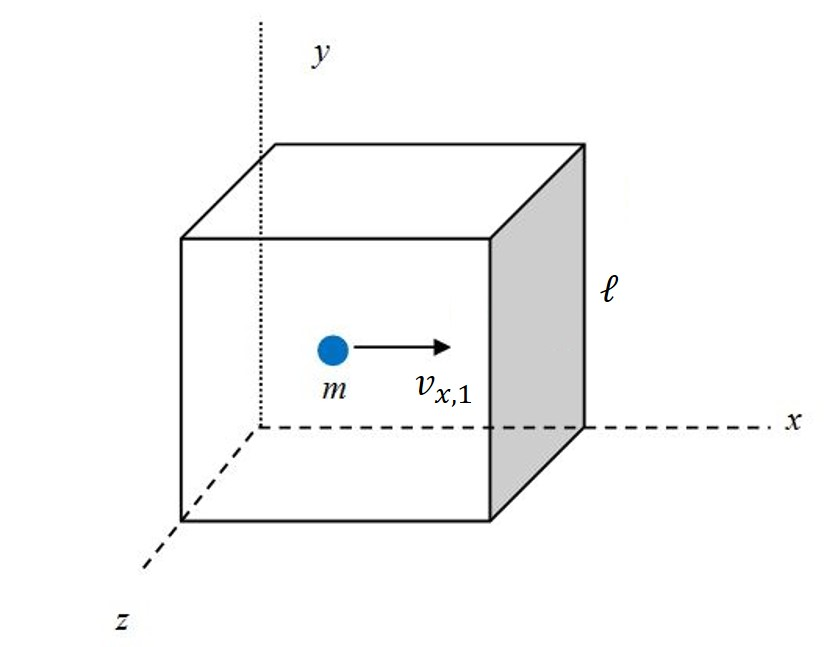
\includegraphics[scale=0.75]{notes/images/Particle-In-Box.JPG}
    \caption{Particle in a container}
\end{figure}
\FloatBarrier

The elastic collision results in a change in momentum of a magnitude of $2 m v_{x, 1}$. This process causes a force to be exerted on the wall by Newton's second law of motion and Newton's third law tells us that the wall exerts an equal and opposite forces on the particle. The particle bounces backwards and forwards between the two walls, exerting a force on each. Since velocity is defined as the first time derivative of displacement, the time $\Delta t$ between two successive collisions with a given contain wall is
\begin{equation*}
    \Delta t = \frac{2 \ell}{v_{x, 1}}.
\end{equation*}
This implies that over a time interval of $\Delta t$, the particle makes a single collision with a given container wall, in which a change of momentum of magnitude $2mv_{x, 1}$ occurs. By Newton's second law of motion, the magnitude of the force exerted by this particle on a given container wall is 
\begin{equation*}
    \| \vec{F}_{x, 1} \| = \frac{m v_{x,1}^2}{\ell}.
\end{equation*}
From the definition of pressure, we can express the pressure $p_1$ exerted by the particle on a given container wall as
\begin{equation*}
    p_1 = \frac{m v_{x,1}^2}{\ell^3}. 
\end{equation*}
Now consider there are $N$ particles, all with velocities along the $x$ dimension. All of these particles moves in a similar motion to the first particle we've been considering. Their velocities will be $v_{x, 1}, v_{x, 2}, \ldots, v_{x, N}$ respectively. Each particle exerts a pressure on the container wall we've been considering in the same way as the first particle. The total pressure $p$ exerted by all $N$ particles on the wall will be the sum of the individual pressure by each particle: 
\begin{align*}
    p &= \sum_{k=1}^N p_k \\
    &= \frac{m}{\ell^3} \sum_{k=1}^N v_{x, k}^2 \\
    &= \frac{m}{\ell^3} N \overline{v_x^2}.
\end{align*}
Applying the following relationship (after considering the fact that we have a collection of particles moving with a range of speeds in random directions):
\begin{equation*}
    \overline{v_x^2} = \overline{v_y^2} = \overline{v_z^2} = \frac{1}{3} \overline{v^2},
\end{equation*}
we find that the total pressure exerted on a single container wall (and indeed on any of the other five walls) is given by
\begin{equation*}
    p = \frac{Nm\overline{v^2}}{3 \ell^3},
\end{equation*}
we also note that $\ell^3$ is equal to the volume of the container $V$, so we have
\begin{equation}
    pV = \frac{1}{3} Nm\overline{v^2}.
\end{equation}

\subsection{Mean Kinetic Energy}

We now have two equations that describe he behaviour of a gas, one based on parameters of a gas and one based on a mechanical model of the particles in the gas. So we have
\begin{align*}
    pV &= nRT = N k_B T \\
    pV &= \frac{1}{3} Nm\overline{v^2}.
\end{align*}
Equating these, we find that
\begin{equation*}
    \frac{1}{2} m \overline{v^2} = \frac{3}{2} k_B T
\end{equation*}
The mean kinetic energy of the gas particles $\overline{E_k}$ is $\frac{1}{2} m \overline{v^2}$, so we have
\begin{equation}
    \overline{E_k} = \frac{3}{2} k_B T.
\end{equation}
Since all other values apart from $T$ remain constant in this equation, it follows that
\begin{equation}
    \overline{E_k} \propto T.
\end{equation}
Note that this only applies when using the absolute temperature (i.e. when the temperature is measured in kelvin). Also based on the assumption that the internal energy $U$ of a gas is entirely kinetic, we find
\begin{equation}
    U = \frac{3}{2} k_B T,
\end{equation}
so the internal energy of a gas is also proportional to it's temperature. 

\section{Material and Properties}
    \clearpage
    
    \chapter{Waves and Optics}
    \section{Wave Phenomena}

\subsection{The Nature of Waves}
\label{subsection:nature-of-waves}
Typically, a wave is a disturbance that propagates through a medium. There are several types of waves we will discuss in this course, including mechanical, electromagnetic, transverse, longitudinal and stationary waves.


\begin{definition}{(\textbf{Propagate})}
\textit{To propagate refers to the transmission of a disturbance from one location to another.}
\end{definition}
\begin{definition}{(\textbf{Medium})}
\textit{Medium (or media) refers to the intervening substance(s) through which a disturbance is transmitted.}
\end{definition}

However, despite the different types of waves we know that waves must transfer energy, momentum, and information, but not mass. 
We will now discuss the different types of waves based on their mediums, wave orientation or energy transfer.

\subsubsection{Types of waves classed by media}
\begin{itemize}
    \item \textbf{Mechanical Waves} \\
    Mechanical waves, such as water or sound waves, travel within, or on the surface of a material. As such, they are characterized as a wave with a medium of \textit{matter}.
    \item \textbf{Electromagnetic Waves}\\
    Electromagnetic waves are waves where electric and magnetic fields are perpendicular to each other and the direction of propagation and require \textit{no medium}. (See section \ref{subsection:electromagnetic-waves})
\end{itemize}
\subsubsection{Types of waves classed by orientation}
\begin{itemize}
    \item \textbf{Transverse Waves} \\
    Transverse waves are those waves in which the disturbance (oscillations) is perpendicular to the direction of propagation. There are two notable features of a transverse waves, the crest and the trough. A crest, sometimes referred to as a peak, is a point of maximal positive displacement from the equilibrium position. Whereas, a trough is a point of maximal negative displacement from the equilibrium position. 
    \item \textbf{Longitudinal Waves} \\
    A longitudinal wave is characterized by the disturbance (oscillations) being parallel to the direction of propagation. In a similar fashion to transverse waves, longitudinal waves have distinct
    regions of disturbance, known as compressions and rarefactions. A compression or condensation is a region where the medium is under compression and a rarefaction or dilation is a region where the medium is under tension.  
    
    \begin{figure}[h!]
        \centering
        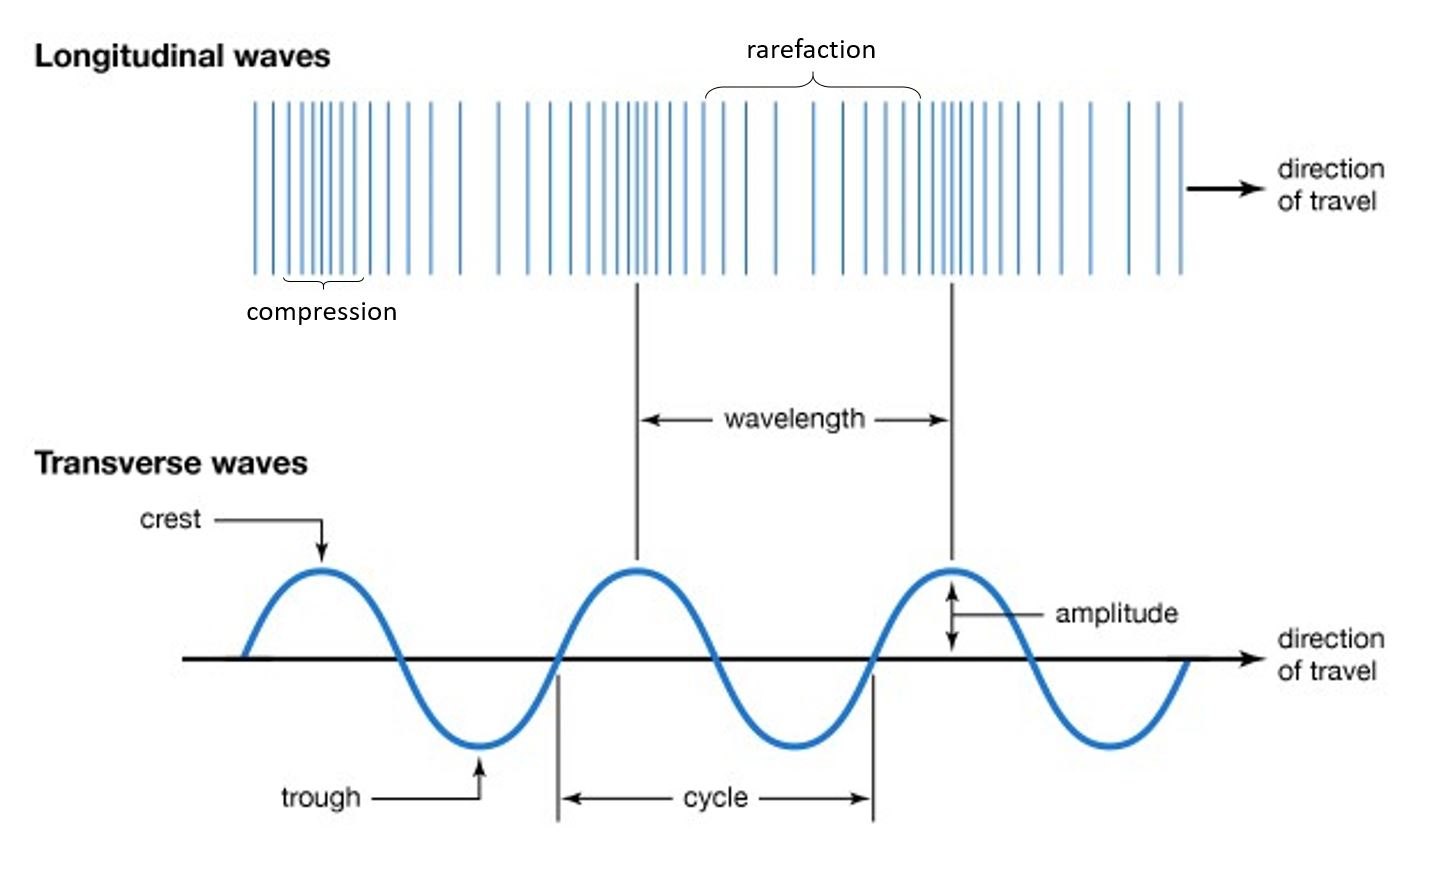
\includegraphics[scale=0.7]{notes/images/Waves-1.JPG}
        \caption{Longitudinal and Transverse waves}
    \end{figure}
    \FloatBarrier
\end{itemize}

\subsubsection{Characteristics of Periodic Waves}
A periodic wave is wave that can be represented by a periodic function of one-dimensional space that moves with constant speed. In this course, we'll typically represent this as a sinusoidal function. 
\begin{itemize}
    \item \textbf{Amplitude} ($A$) \\
    The maximum absolute value of a periodically varying quantity. In longitudinal waves it might be pressure or displacement from the equilibrium position. In a transverse wave it is displacement. In this course we will generally stick to the convention that amplitude is the maximum displacement from the equilibrium position.
    \item \textbf{Period} ($T$) \\
    The time between successive cycles of a wave. The time period can be calculated using 
    \begin{equation}
        T = \frac{t}{n},
    \end{equation}
    where $t$ is the time taken for $n$ cycles to occur. The unit of period is \textbf{seconds} ($s$)
    \item \textbf{Frequency} ($f$) \\
    The number of cycles per seconds, hence the frequency can be calculated using
    \begin{equation}
        f = \frac{n}{t},
    \end{equation}
    where $t$ is the time taken for $n$ cycles to occur. Thus frequency and time period are the reciprocal of one another, that is
    \begin{equation}
        f = \frac{1}{T} \text{ and } T = \frac{1}{f}.
    \end{equation}
    The unit of frequency is the \textbf{hertz} ($Hz$).
    \item \textbf{Phase} ($\phi$) \\
    Phase difference is said to be the difference in displacement of two points along the same wave or the difference in displacement of two points on different waves. The phase difference between two points on a wave separated by a distance of $x$ metres is given by 
    \begin{equation}
        \phi = \frac{x}{\lambda} 2\pi,
    \end{equation}
    where $\lambda$ is the wavelength of the wave. So phase is an angular quantity measured in \textbf{radians}.
    
    Two points are said to be \textbf{in phase} if they are separated by one complete cycle, that is if $\phi \pmod{2\pi} \equiv 0$, in a similar fashion, two points are said to be \textbf{out of phase} if they are separated by half a cycle, that is if $\phi \pmod{2\pi} \equiv \pi$. 
    \item \textbf{Wavelength} ($\lambda$) \\
    The distance between adjacent points in phase. In short, the wavelength is the length of one cycle. Wavelength is measured in \textbf{metres} ($m$).
    \item \textbf{Speed} ($v$) \\
    Waves propagate with a finite speed, sometimes called the wave speed, which has a number of factors:
    \begin{itemize}
        \item the type of wave
        \item the composition of the medium
        \item the state of the medium
    \end{itemize}
    From the definition of speed, it follows that the wave speed is the produce of frequency and wavelength for periodic waves, that is 
    \begin{equation}
        v = f \lambda.
    \end{equation}
    The unit for wave speed is the \textbf{metre per second} ($ms^{-1}$)
\end{itemize}

\subsection{Interference and Superposition}

For modelled by wave functions (we note that the functions themselves are irrelevant), if  $f_1(x, t)$ and $f_2(x,t)$ are waves, then so is
\begin{equation}
    f(x, t) = f_1(x, t) + f_2(x, t)
\end{equation}
which is called the \textit{superposition} of the waves $f_1$ and $f_2$. Waves add algebraically. This simple law is what gives rise to the fact that waves pass through each other without affecting each other. 

\begin{theorem}{(\textbf{Principle of Superposition})}
\textit{The principle of superposition states that when two waves meet at a point the resultant displacement at that point is equal to the sum of the displacements of the individual waves.}
\end{theorem}

Before giving an example of superposition, let us elaborate on the notation we introduced above. Waves can be modelled by linear displacement functions in the form $\vec{s} = f(x, t)$ where $\vec{s}$ is the displacement, the plot of a function of $x$ at a fixed time $t$ is known as the ``snapshot'' and the plot of a function of $t$ at fixed $x$ is the displacement of experienced by a particle $p$ at position $x$ as time passes.

Suppose $y_1$ and $y_2$ are waves with similar shapes, with $y_2$ traveling to the right, but $y_2$ traveling to the left and upside down. Then superposition is
\begin{equation*}
    y(x, t) = y_1(x, t) + y_2(x, t).
\end{equation*}
A snapshot at a fixed time $t$ looks like the plot below:
\begin{figure}[h!]
    \centering
    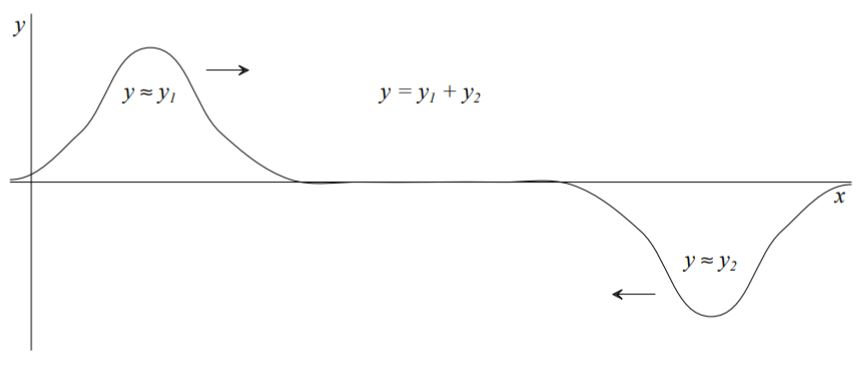
\includegraphics{notes/images/Superposition-1.JPG}
\end{figure}
\FloatBarrier
\noindent At some time $t_0$ later, the two waves will be exactly opposite, that is
\begin{equation*}
    y_1 (x, t_0) = -y_2(x, t_0)
\end{equation*}
and so $y(x, t_0) = 0$. At $t = t_0$, the snapshot is
\begin{figure}[h!]
    \centering
    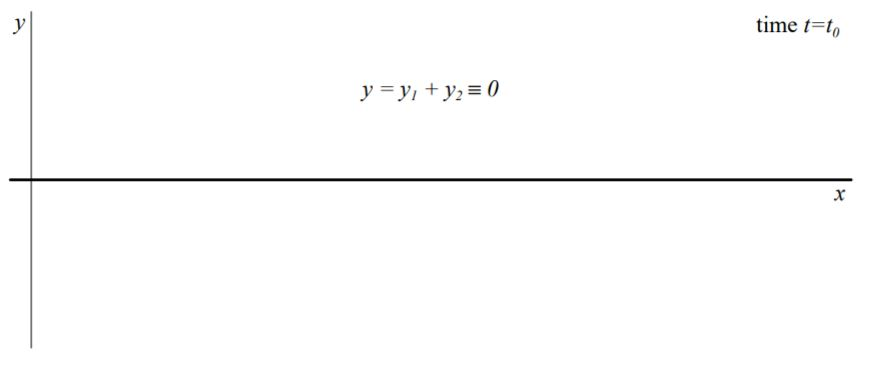
\includegraphics{notes/images/Superposition-2.JPG}
\end{figure}
\FloatBarrier
\noindent Somewhat later still, say at $t = t_1$, the waves have passed through each other, and the snapshot is
\begin{figure}[h!]
    \centering
    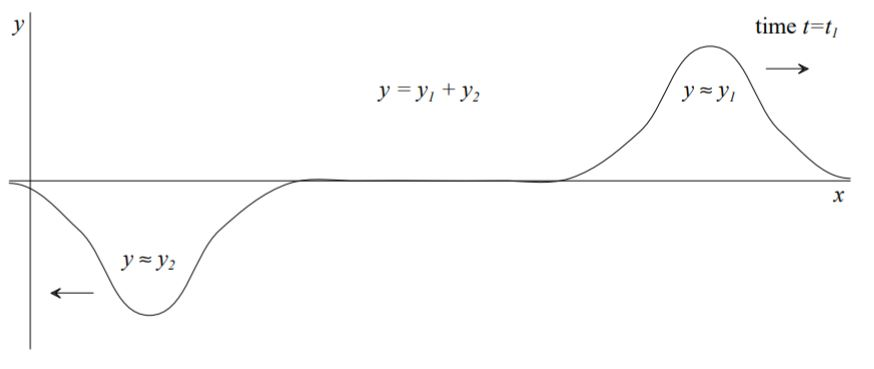
\includegraphics{notes/images/Superposition-3.JPG}
\end{figure}
\FloatBarrier

The superposition of these waves \textbf{interfere destructively}, that is when two waves superpose resulting in the cancellation of their displacement, i.e when the negative displacement of one wave coincides with the positive displacement of the other, which occurs when they are \textbf{antiphase}. The term \textbf{interfere} just refers to two waves superposing. The superposition of two waves that are in \textbf{phase} will \textbf{interfere constructively}, that is when two waves superpose resulting in a displacement with an increase amplitude. 

When two waves interfere, the intensity is affected. We will learn later on that $I_v \propto A^2$, where $I_v$ denotes intensity. In the case of constructive interference, an increase in intensity will occur which can be demonstrated by sounds  becoming ``louder'' and light becoming ``brighter''. The converse is true for destructive interference, that is a decrease in intensity will occur, i.e sounds are quieter and light is dimmer. 

\subsection{Diffraction and Reflection}

\textbf{Diffraction} is a property unique to waves; it is the bending or spreading of a wave around an obstacle or through an opening. The effects of diffraction are most apparent when the size of the obstacle or opening $a$ is approximately equal to the wavelength of the wave $\lambda$. This is why sound diffracts when it passes through a doorway, since the wavelength of the sound is similar to the width of the doorway. However, light has a much small wavelength, so it does not diffract through such a large gap. (See figure \ref{fig:diffraction-patterns}) 

\begin{figure}[h!]
    \centering
    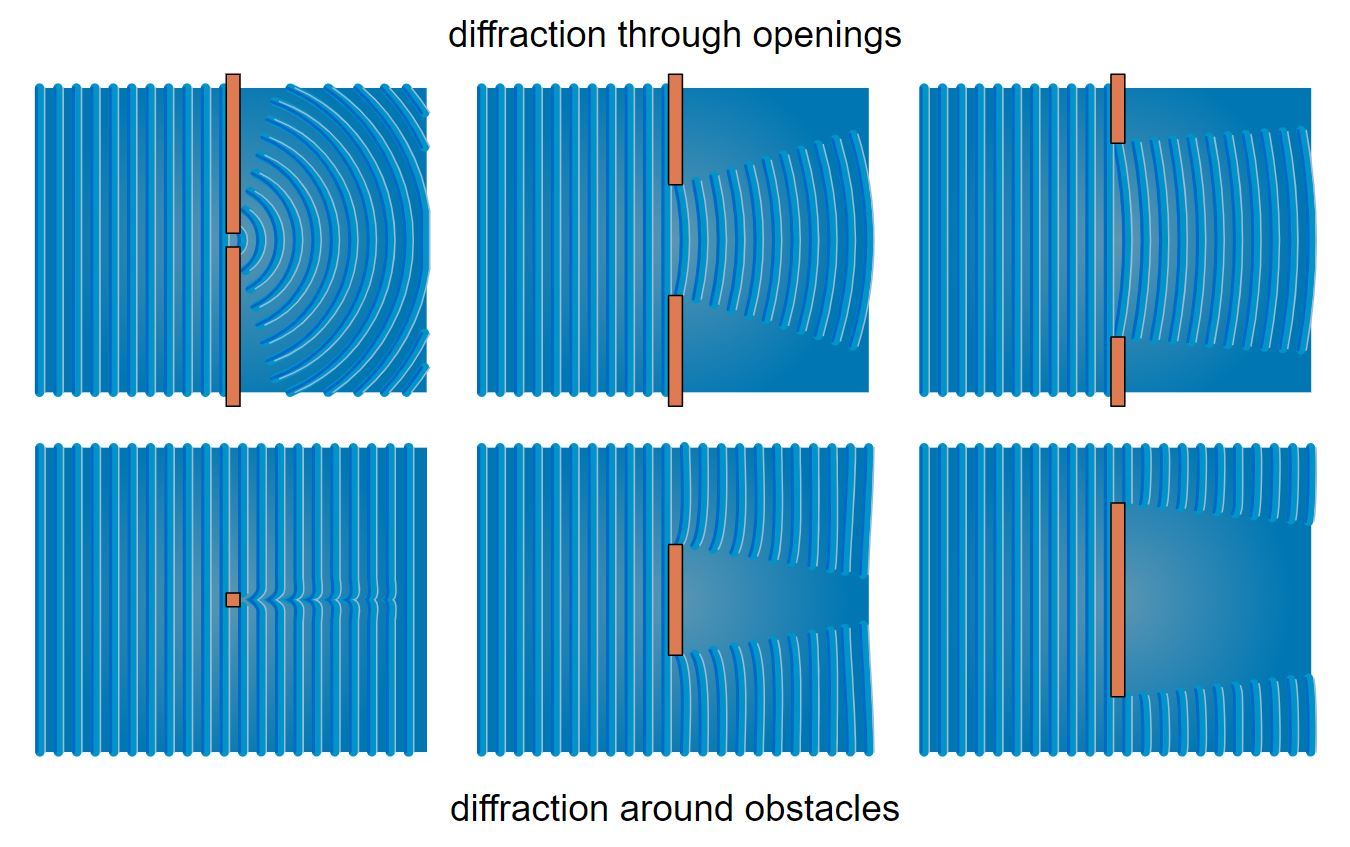
\includegraphics[scale=0.7]{notes/images/Diffraction-1.JPG}
    \caption{Diffraction Patterns}
    \label{fig:diffraction-patterns}
\end{figure}
\FloatBarrier

Typically when a wave travels through a medium and meets the boundary of another medium, it is \textbf{reflected}. The reflected wave does or does not undergo a phase change of $\pi$ radians depending on the boundary media. To describe this situation for strings, we will consider two cases where the boundary is fixed and where it is free to move. 

In the first case, suppose that one end of the string is tied to wall, as shown below. When the shape incidence from the left reaches the wall, the tension in the string tends to pull upwards on the wall. From Newton's third law, the reaction force exerted by the wall on the string is then downwards, making the reflected shape inverted thus undergoing a phase change of $\pi$ radians. 

\begin{figure}[h!]
    \centering
    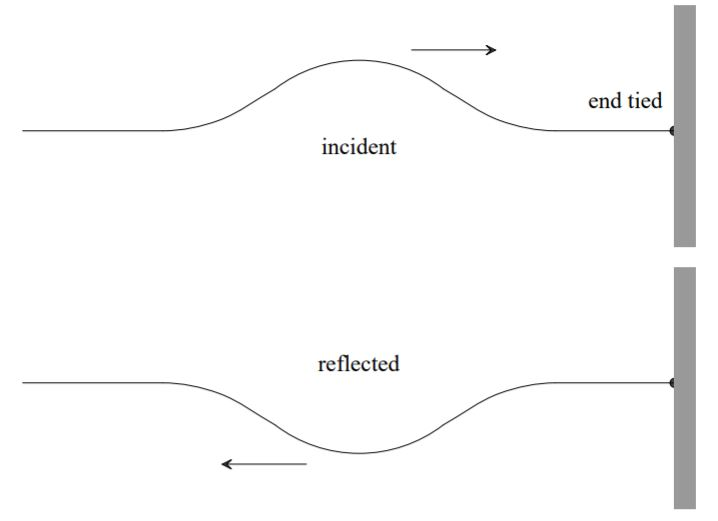
\includegraphics[scale=0.9]{notes/images/Reflection-1.JPG}
\end{figure}
\FloatBarrier

In the second case, the end of the string is tied to a frictionless ring, free to move up and down on a rod, as shown below. This time the pulse incident from the left just moves the ring upwards when it reaches the wall, making the reflected shape also upward, not inverted. 

\begin{figure}[h!]
    \centering
    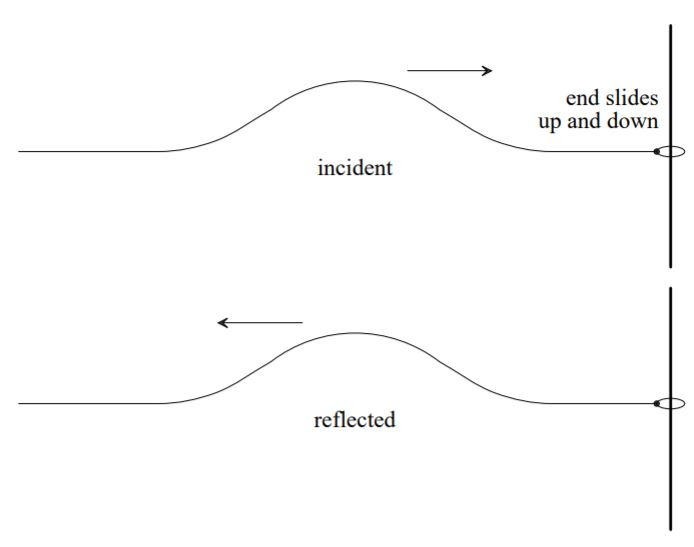
\includegraphics[scale=0.9]{notes/images/Reflection-2.JPG}
\end{figure}
\FloatBarrier

\begin{definition}{(\textbf{Law of Reflection})}
\textit{The law of reflection states the angle which the incident ray makes with the normal is equal to the angle which the reflected ray makes to the same normal. Mathematically, $\theta_i = \theta_r$.}
\begin{figure}[h!]
    \centering
    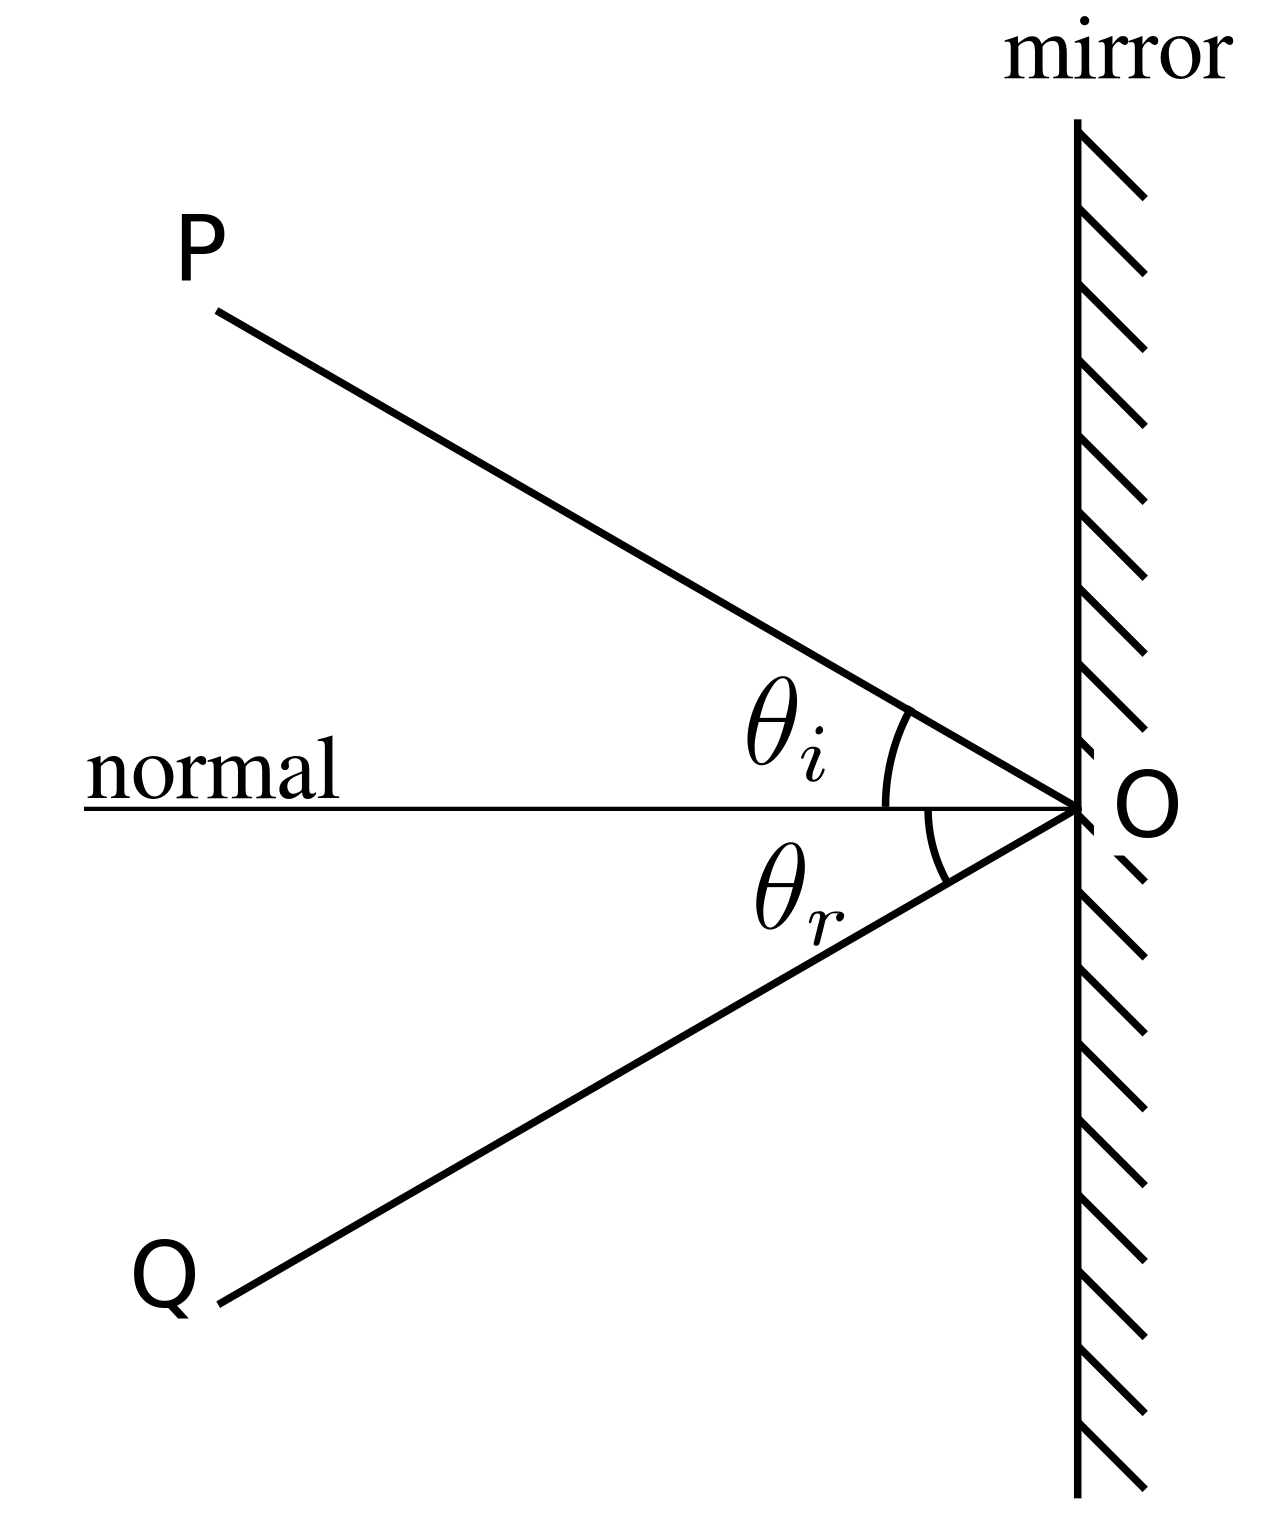
\includegraphics[scale=0.09]{notes/images/Law-Of-Reflection.JPG}
\end{figure}
\FloatBarrier

\end{definition}

\subsection{Polarization}

The phenomenon of \textbf{polarization} is something that only transverse waves exhibit. A wave in which the oscillations take place in a number of places is said to be \textbf{unpolarized}, while a wave in which the oscillations occur in one plane is \textbf{plane polarized} in that direction. Electromagnetic waves are transverse waves, and may be polarized. Unpolarized electromagnetic waves can be polarized using filters called \textbf{polarizers} or \textbf{polaroids}. A common use of polarizers is to prevent electromagnetic waves used in communications interfering with each other. 

\begin{figure}[h!]
    \centering
    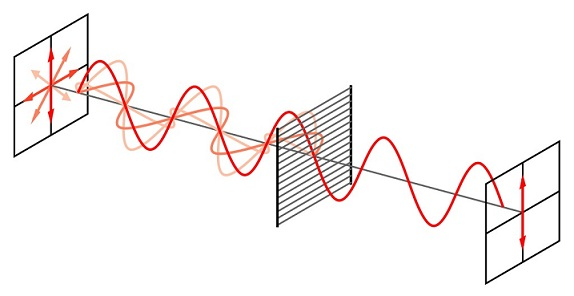
\includegraphics[scale=0.75]{notes/images/Polarization-1.JPG}
    \caption{A unpolarized and plane polarized wave}
\end{figure}
\FloatBarrier

\subsubsection{Malus' Law}

Suppose we have a second polaroid whose vertical makes an angle $\theta$ with the first one. The intensity of the wave that exits the second polaroid $I$ is given by
\begin{equation}
    I = I_0 \cos^2 \theta,
\end{equation}
where $I_0$ is the intensity of the wave exiting the first polaroid. 

\begin{figure}[h!]
    \centering
    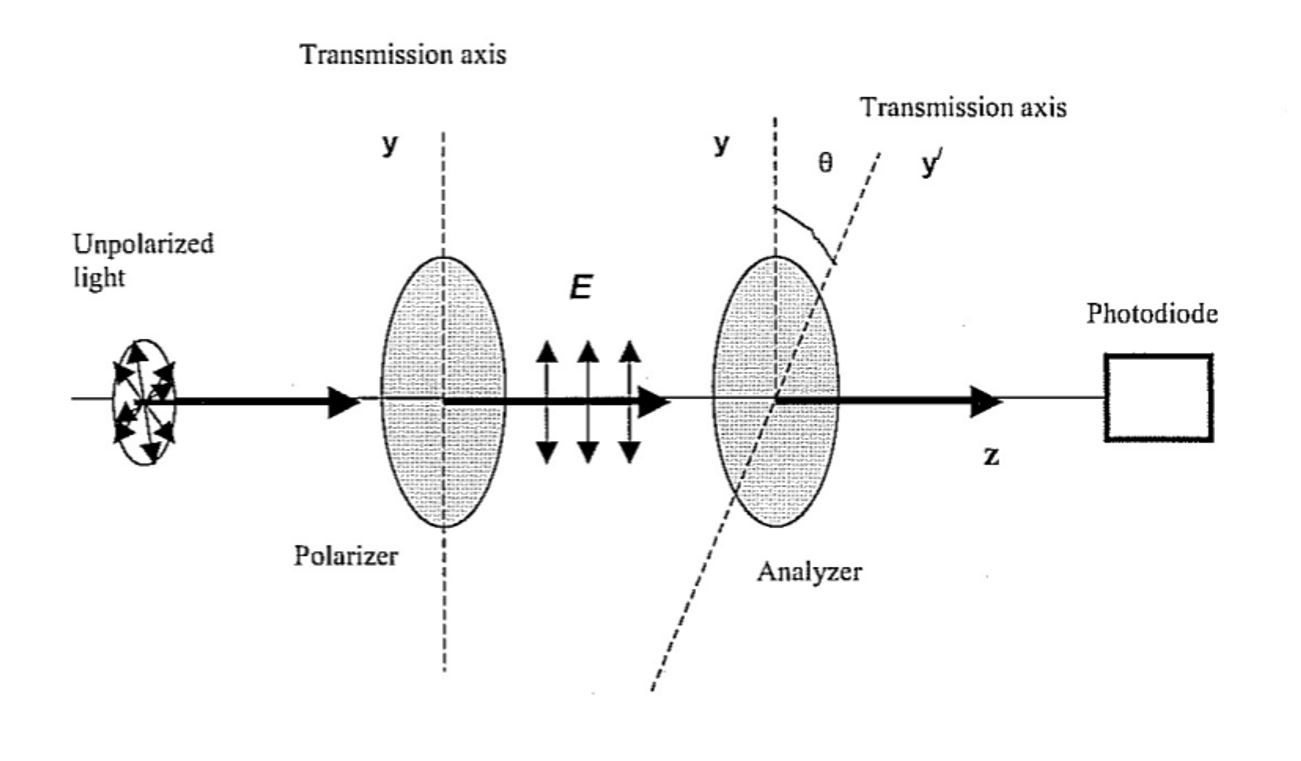
\includegraphics[scale=0.75]{notes/images/Malus-Law.JPG}
\end{figure}
\FloatBarrier

\subsection{Intensity}
\label{subsection:intensity}

The \textbf{intensity} $I_v$ of a wave is the time-averaged power $\langle P \rangle$ it transfers per unit of area $A$ through some region of space. The traditional way to indicate the time-average value of a varying quantity is to enclose it in the angled brackets $\langle \hspace{1mm} \rangle$. So the equation for intensity is
\begin{equation}
    I_v = \frac{\langle P \rangle}{A}
    \label{eq:intensity}
\end{equation}
measured in \textbf{watts per square metre} ($Wm^{-2}$). Intensity for \textit{mechanical waves} can be related to the density of the medium and the speed, frequency and amplitude of the wave via a long and horrible derivation. This equation or it's related derivation isn't required for A2 Physics, however, it will allow us to understand the factors that affect intensity. 

\begin{equation}
    I_v = 2 \pi^2 \rho f^2 v A^2,
\end{equation}
where $\rho$ denotes the density of the medium, $v$ is wave speed, $f$ is frequency and $A$ is amplitude. 

\subsubsection{Factors affecting mechanical waves}
\begin{itemize}
    \item $I_v \propto \rho$ \\
    The denser the medium, the more intense the wave. A dense medium packs more mass, since kinetic energy is proportional to mass, it follows that power is proportional to mass and therefore intensity is proportional to mass, thus rationalizing this relationship.
    \item $I \propto f^2$ \\
    The more cycles per unit of time, the more energy transferred. Therefore the more frequently a wave vibrates the medium, the more intense the wave is.
    \item $I \propto v$ \\
    The faster the wave travels, the more quickly it transmits energy. Since power is the rate of energy transferred, it follows that intensity is proportional to wave speed.
    \item $I \propto A^2$ \\
    Decreased amplitude means a reduced average speed of the oscillating \textit{particles} (considering the frequency is constant). Since kinetic energy is proportional to speed squared, it follows that intensity is directly proportional to the square of the amplitude. We should note that this is also implied by simple harmonic motion, since it's energy depends on the square of the oscillations amplitude. The relationship also applied to waves in general and therefore also applies to electromagnetic waves.
\end{itemize}

\subsubsection{Intensity and Distance}

Consider a circular wave, like the wave produced from dropping a stone in water, from a source. The wave carries energy with it which is spread over a larger and larger area as the wave spreads out. The radiant power from this wave is uniformly spread over the surface of a sphere with radius $r$. 

So the total radiant power $P$ at a distance $r$ from the source is spread over an area of a sphere $4\pi r^2$. Applying this to equation \ref{eq:intensity}, we have
\begin{equation}
    I_v = \frac{\langle P \rangle}{4 \pi r^2}.
\end{equation}
From this relationship, it follows that intensity is inversely proportional to the distance from the source.
\begin{equation}
    I_v \propto \frac{1}{r^2}.
\end{equation}

\section{Sound}

\subsection{Stationary Waves}

\textbf{Stationary waves}, also known as standing waves, refers to a wave that is \textit{not} progressive and a wave where the positions of the peaks and troughs are not moving. This is because a stationary wave is not a single wave, but the superposition of two progressive waves with the same frequency travelling in opposite directions. The easiest way to form the pair of progressive waves is by reflecting an incident wave at the boundary of media.

As they have the same frequency, at certain points they are in phase, forming \textbf{antinode}; an antinode is a point where the displacement is always at a maximum due to constructive interference.  At other points when the two waves are in antiphase, a \textbf{node} is formed - a point where the displacement is always zero (or at a minima). 

\begin{figure}[h!]
    \centering
    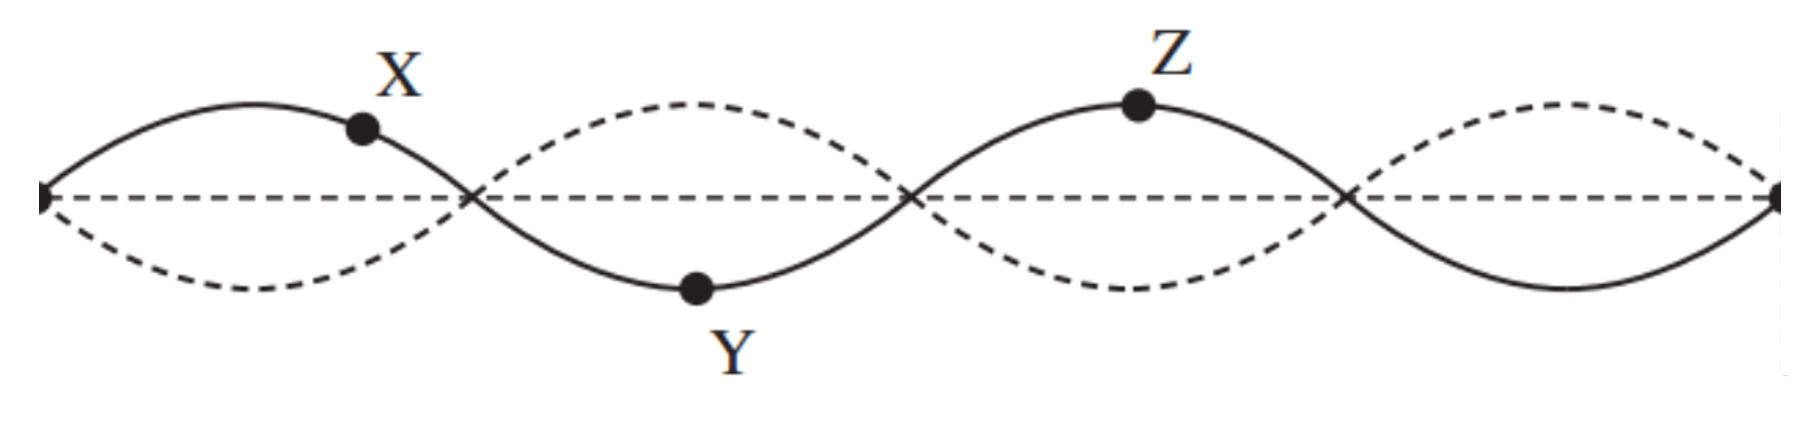
\includegraphics[scale=0.5]{notes/images/Stationary-Wave-Phase-Difference.JPG}
    \label{fig:stationary-wave}
    \caption{A stationary wave}
\end{figure}
\FloatBarrier

The separation between two adjacent nodes or antinodes is equal to half of the wave length of the original progressive wave and the frequency of the standing wave is equal to the frequency of the original progressive wave. 

\begin{table}[h!]
    {
        \begin{tabular}{l|p{0.4\linewidth}|p{0.4\linewidth}}
            \hspace{1mm} & Progressive wave & Stationary wave  \\
            \hline
            Energy transfer & Energy transferred in the direction of the wave. & No net energy transfer \\
            Wavelength & The distance in which the phase changes by $2\pi$ & Twice the distance between two adjacent nodes (or antinodes) is equal to the wavelength of the progressive wave that forms the stationary wave  \\
            Phase difference & The phase changes across one complete cycle of the wave & All parts of the wave between a pair of nodes are in phase, and on the other sides of the nodes they are in antiphase. For example, in figure \ref{fig:stationary-wave} the points X and Z are in phase, whereas X and Y are in antiphase. \\
            Amplitude & All peaks / troughs have the same amplitude (assuming no energy is lost) & Maximum amplitude occurs at antinodes
        \end{tabular}
    }
\end{table}
\FloatBarrier

\subsection{Harmonics}

Any system in which stationary waves can form has numerous frequencies in which a stationary wave can form. The set of all possible stationary waves are known as the \textbf{harmonics} of a system. The simplest of the harmonics is called the \textbf{fundamental} or \textbf{first harmonic}, which has an associated \textit{fundamental} frequency denoted $f_0$ or $f$. Subsequent stationary waves called the second harmonic, third harmonic, etc whose frequencies are multiples of the fundamental frequency, that is the second harmonic has a frequency of $2f_0$, the third harmonic has a frequency of $3f_0$, etc. So what wavelengths will form stationary waves in a simple, one-dimensional system with these frequencies? There are three simple cases  

In the first case, suppose that a medium is bounded such that its opposite ends can be considered fixed, it follows that nodes will then form at the ends. The simplest stationary wave that can form under these circumstances has one antinodes in the middle. The distance between the bounds is half a wavelength. The same argument can be applied to the second harmonic, finding the distance between the bounds is a wavelength. It should become obvious that a pattern begins to emerge (see figure \ref{fig:harmonic-1}), that is for the $n^{th}$ harmonic with frequency $nf$ the wavelength is given by $\lambda = \frac{2}{n} L$, where $L$ is the distance between the bounds.  

\begin{figure}[h!]
    \centering
    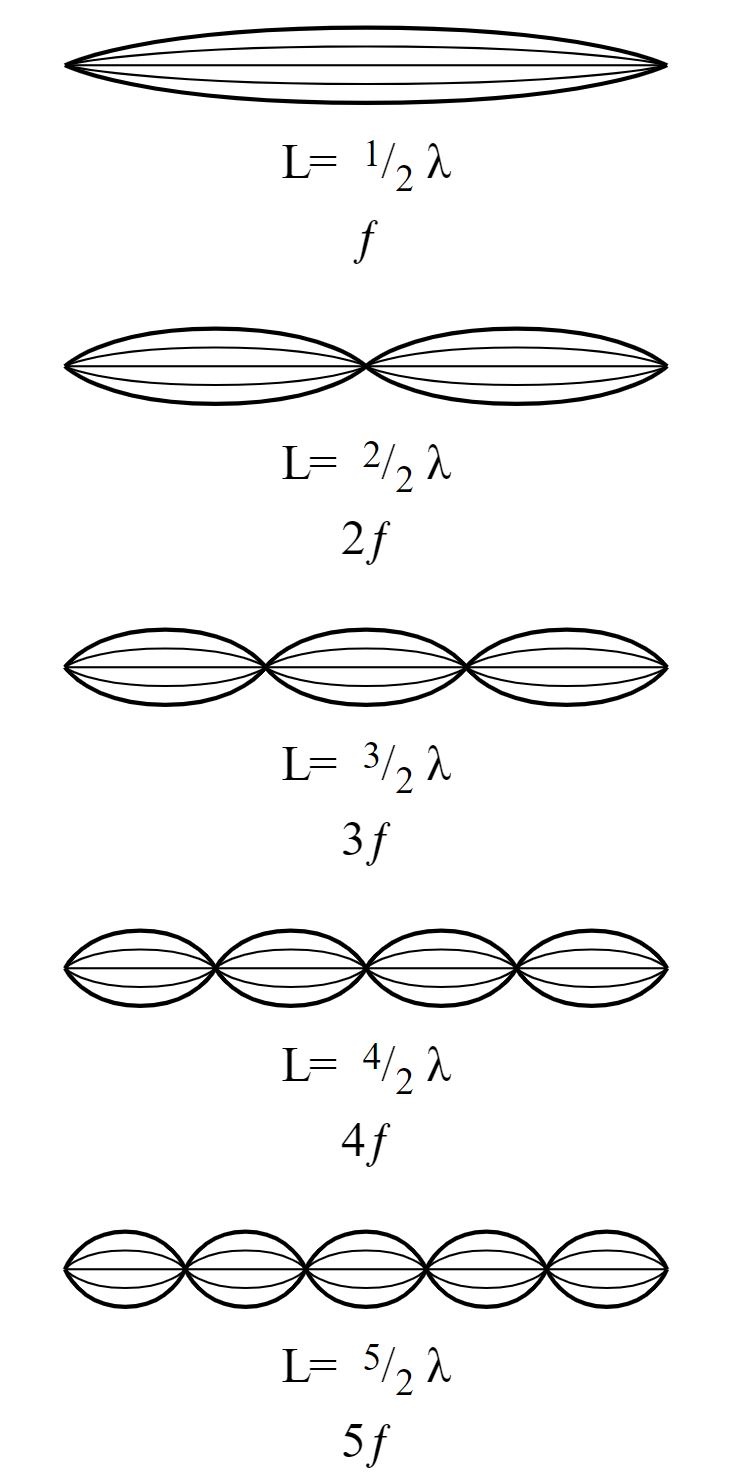
\includegraphics[scale=0.5]{notes/images/Harmonic-1.JPG}
    \caption{Harmonics with fixed ends}
    \label{fig:harmonic-1}
\end{figure}
\FloatBarrier

In the second case, suppose that a medium is bounded such that its opposite ends can be considered free, so antinodes will form at the ends. The simplest stationary wave that can form under these circumstances has one node in the middle. The distance between the bounds is half the wavelength. To make the next possible stationary wave, place another antinode in the center. We now have one whole wavelength. It should become apparent that we will get the same relationships for the stationary waves formed between two free ends that we have for two fixed ends. The only difference is that nodes are replaced with antinodes and vice versa. So for the $n^{th}$ harmonic with frequency $nf$ the wavelength is given by $\lambda = \frac{2}{n} L$, where $L$ is the distance between the bounds. 

\begin{figure}[h!]
    \centering
    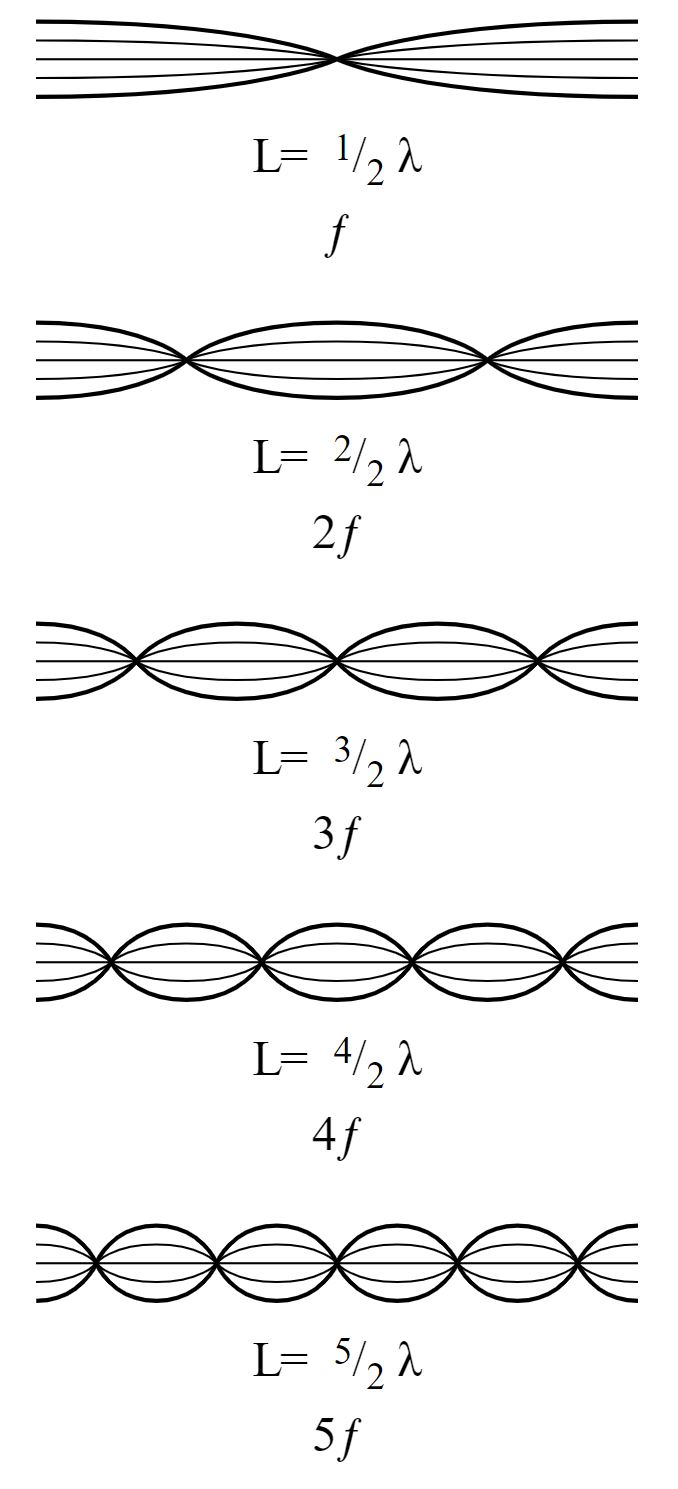
\includegraphics[scale=0.5]{notes/images/Harmonic-2.JPG}
    \caption{Harmonics with free ends}
\end{figure}
\FloatBarrier

In the third and final case, suppose that a medium has one fixed end and one free end. A node will always form at the fixed end while an antinode will always form at the free end. The simplest stationary wave that can form under these conditions has a wavelength that is 4 times the distances between the bounds. The next possible stationary wave is formed by adding a node and an antinode, with wavelength that is four thirds of the distance between the bounds. Repeating this procedure, we begin to notice a pattern; for the $n^{th}$ harmonic with frequency $nf$ the wavelength is given by $\lambda = \frac{4}{n} L$. However, we note that the frequencies of the harmonics are always odd multiples of the fundamental frequency and therefore we can only have odd harmonics, that is $n \in \mathbb{Z}_{odd}^+$

\begin{figure}[h!]
    \centering
    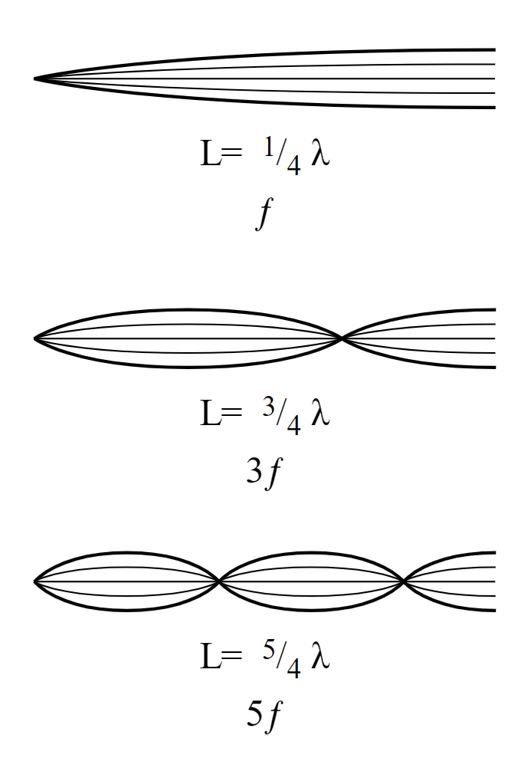
\includegraphics[scale=0.55]{notes/images/Harmonic-3.JPG}
    \caption{Harmonics with one fix end and one free end}
\end{figure}
\FloatBarrier

\section{Optics}

\subsection{Electromagnetic Waves}
\label{subsection:electromagnetic-waves}

As stated in section \ref{subsection:nature-of-waves}, electromagnetic (EM) waves are those waves in which electric and magnetic fields are perpendicular to each other as well as the direction of propagation and requires no medium. 

\noindent The properties of EM waves are as follows:
\begin{itemize}
    \item These waves are transverse in nature
    \item These waves propagate through a vacuum with the speed of light
    \item The speed squared of an electromagnetic wave is given by 
    \begin{equation}
        c^2 = \frac{1}{\varepsilon_0 \mu_0},
    \end{equation}
    where $\varepsilon_0$ is the permittivity of a vacuum and $\mu_0$ is the permeability of a vacuum.
    \item The oscillating electric and magnetic fields are self sustaining if they are perpendicular to one another and the direction of propagation, and are in phase.
\end{itemize}

\begin{figure}[h!]
    \centering
    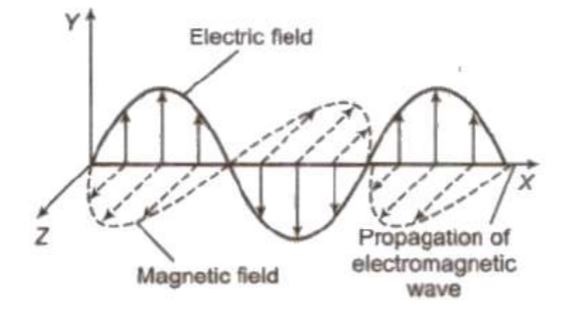
\includegraphics{notes/images/EM.JPG}
    \caption{An EM wave}
\end{figure}
\FloatBarrier

\subsubsection{The Electromagnetic Spectrum}

The arranged array of electromagnetic radiations in the sequence of their wavelength of frequency is called the \textbf{electromagnetic spectrum} and ranges from \textbf{radio waves} with the longest wavelength to \textbf{gamma rays} with the shortest wavelength. 

\begin{figure}[h!]
    \centering
    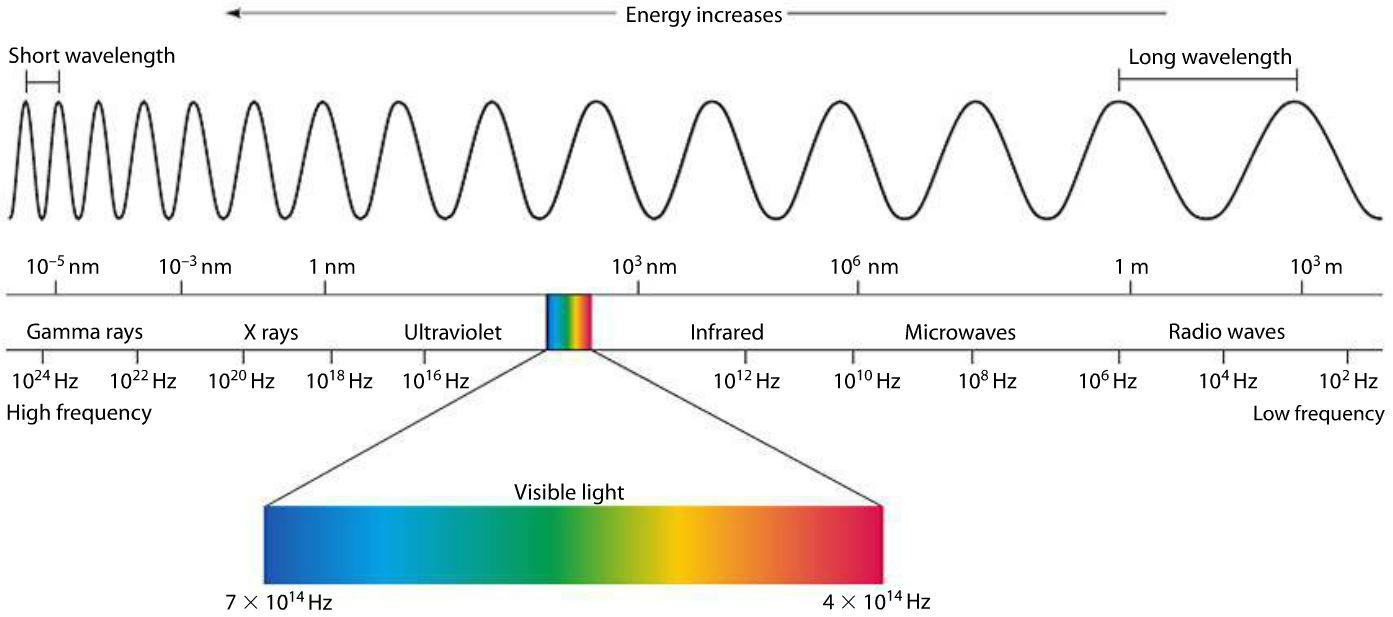
\includegraphics[scale=0.4]{notes/images/EM-Spectrum.JPG}
    \caption{The electromagnetic spectrum}
\end{figure}
\FloatBarrier

\subsection{Refraction}

\textbf{Refraction} occurs when a wave changes direction at the boundary of media. This is due to a change in wavespeed when passing from one medium to another. 

If the wave slows down it will refract towards the normal, whereas if the wave speeds up it refracts away from the normal, as shown below.


\begin{figure}[h!]
    \centering
    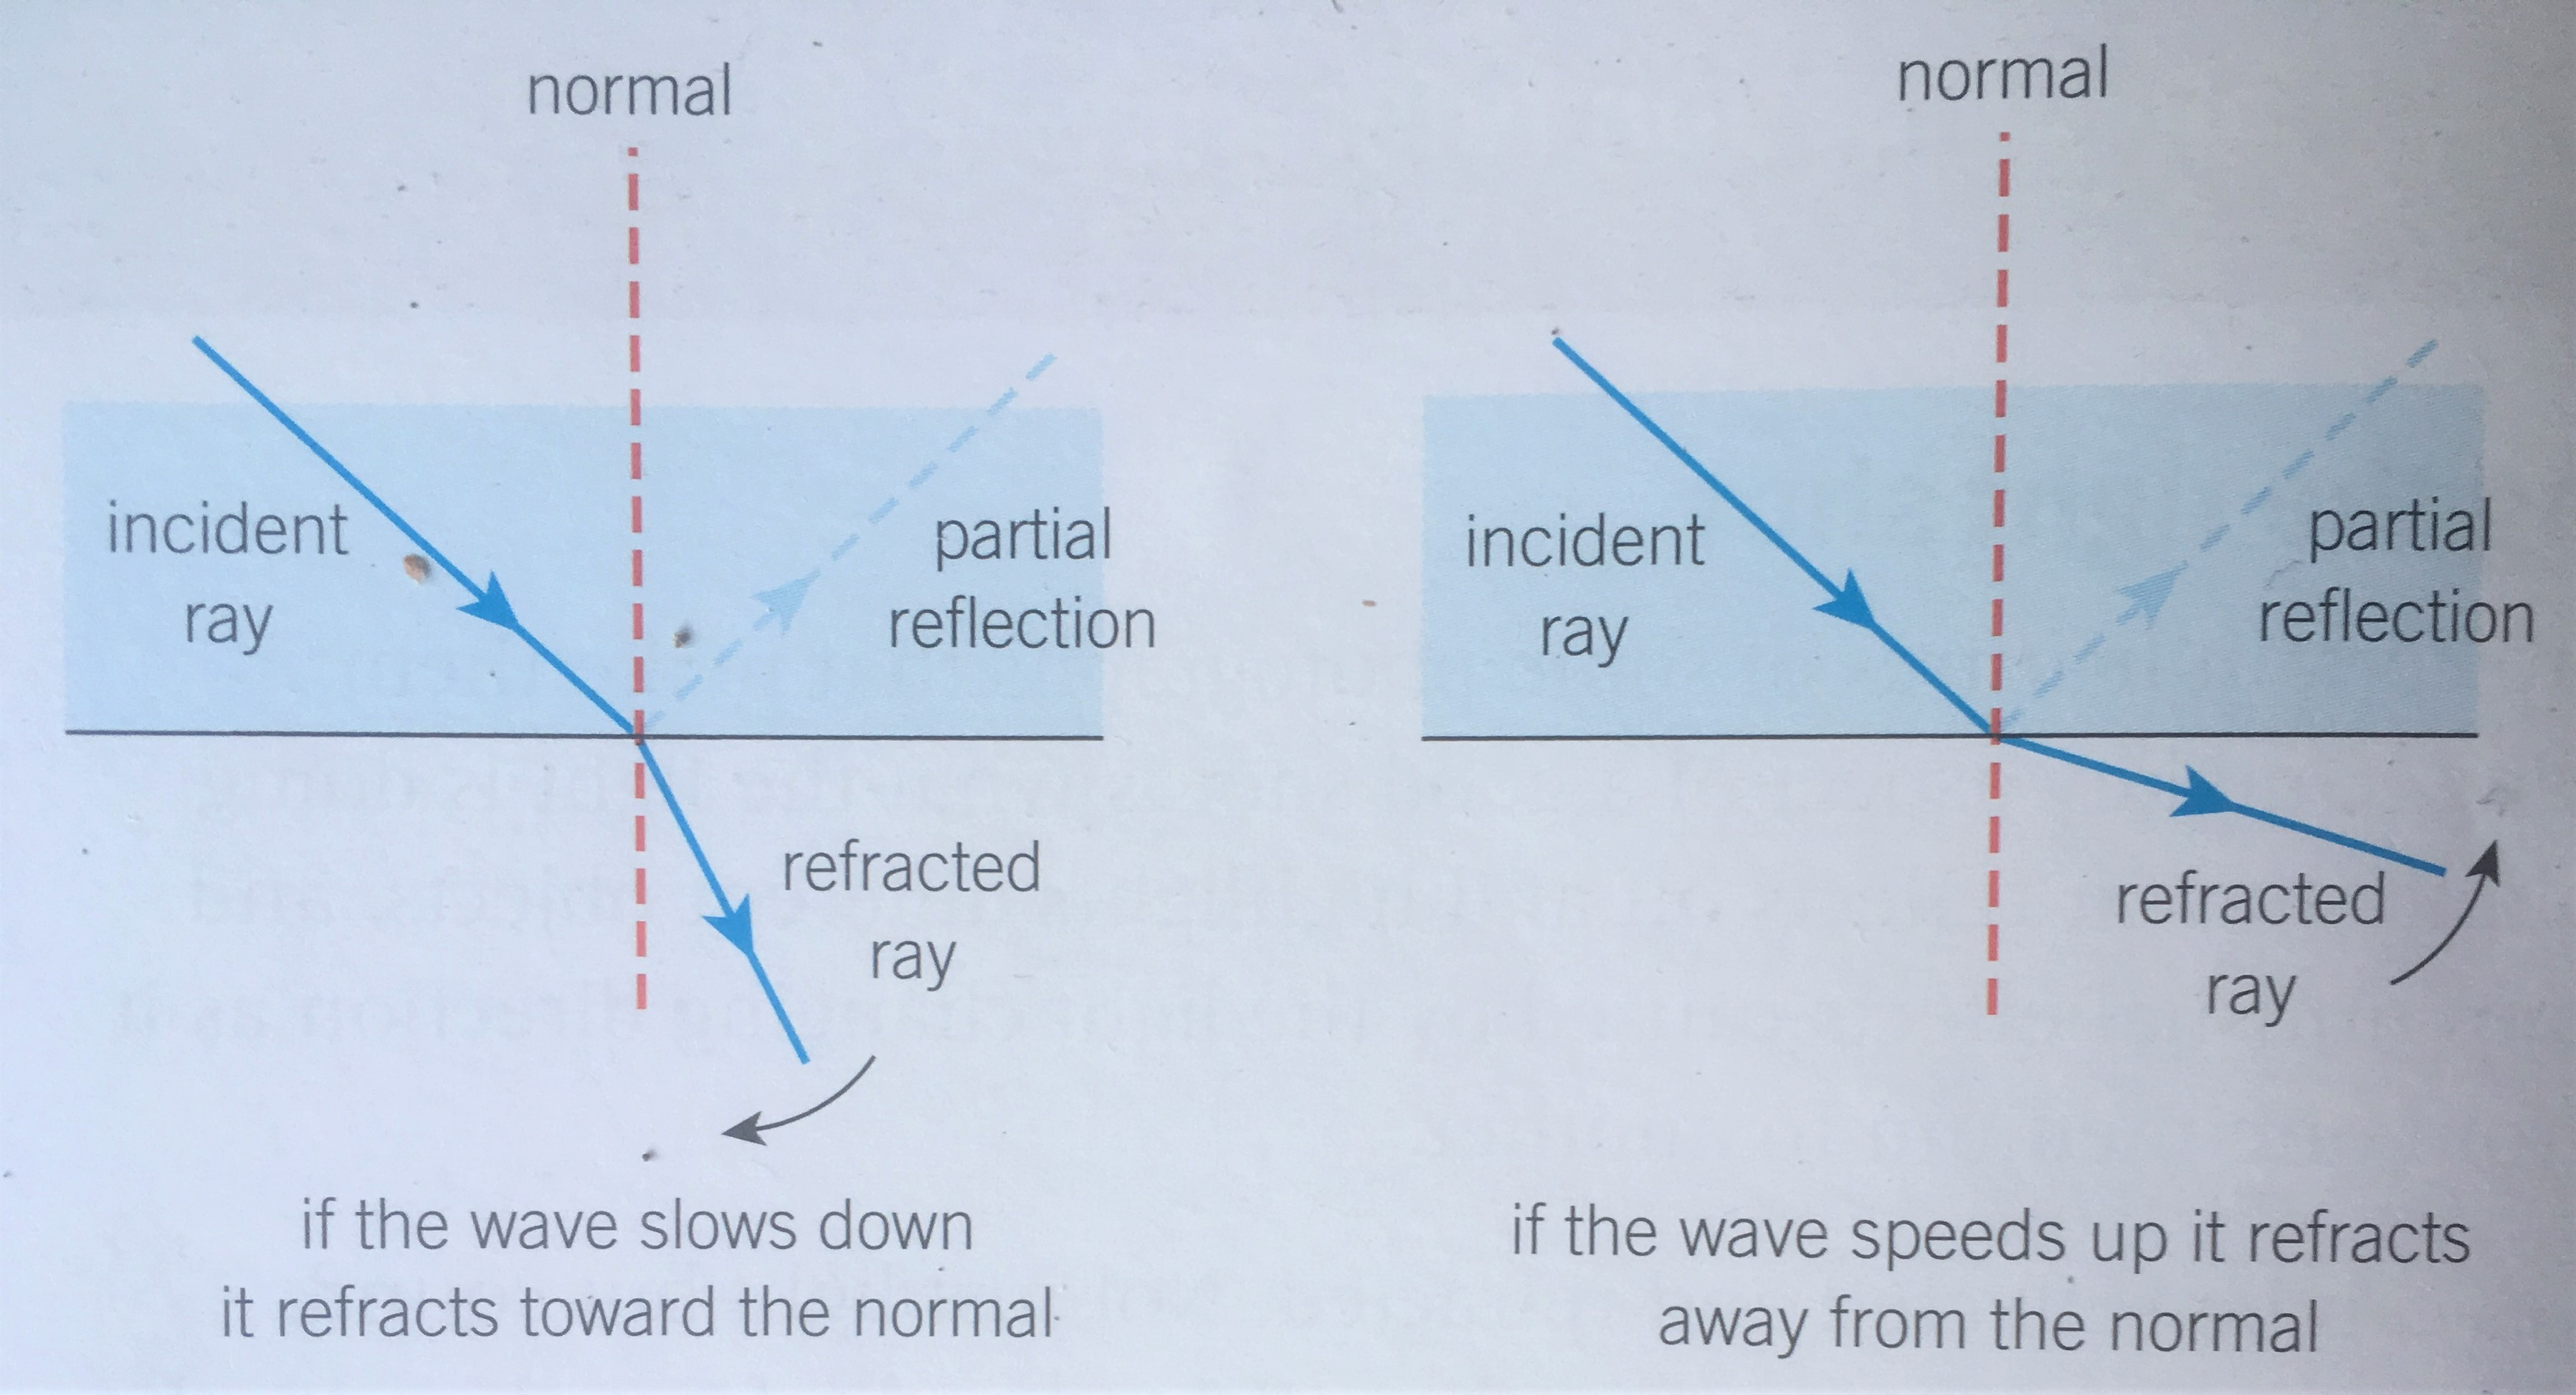
\includegraphics[scale=0.09]{notes/images/Refraction-2.JPG}
\end{figure}
\FloatBarrier


Snell's law (named after Willebrord Snellius) describes the relationship between the angles of incidence and refraction. The law states that the ratio of the sines of the angles of incidence and refraction is equivalent to the ratio of the velocities, wavelengths or equivalent to the reciprocal of the ratios of indices of refraction, that is:
\begin{equation}
    \frac{\sin \theta_1}{\sin \theta_2} = \frac{n_2}{n_1} = \frac{v_1}{v_2} = \frac{\lambda_1}{\lambda_2}. 
\end{equation}

\begin{figure}[h!]
    \centering
    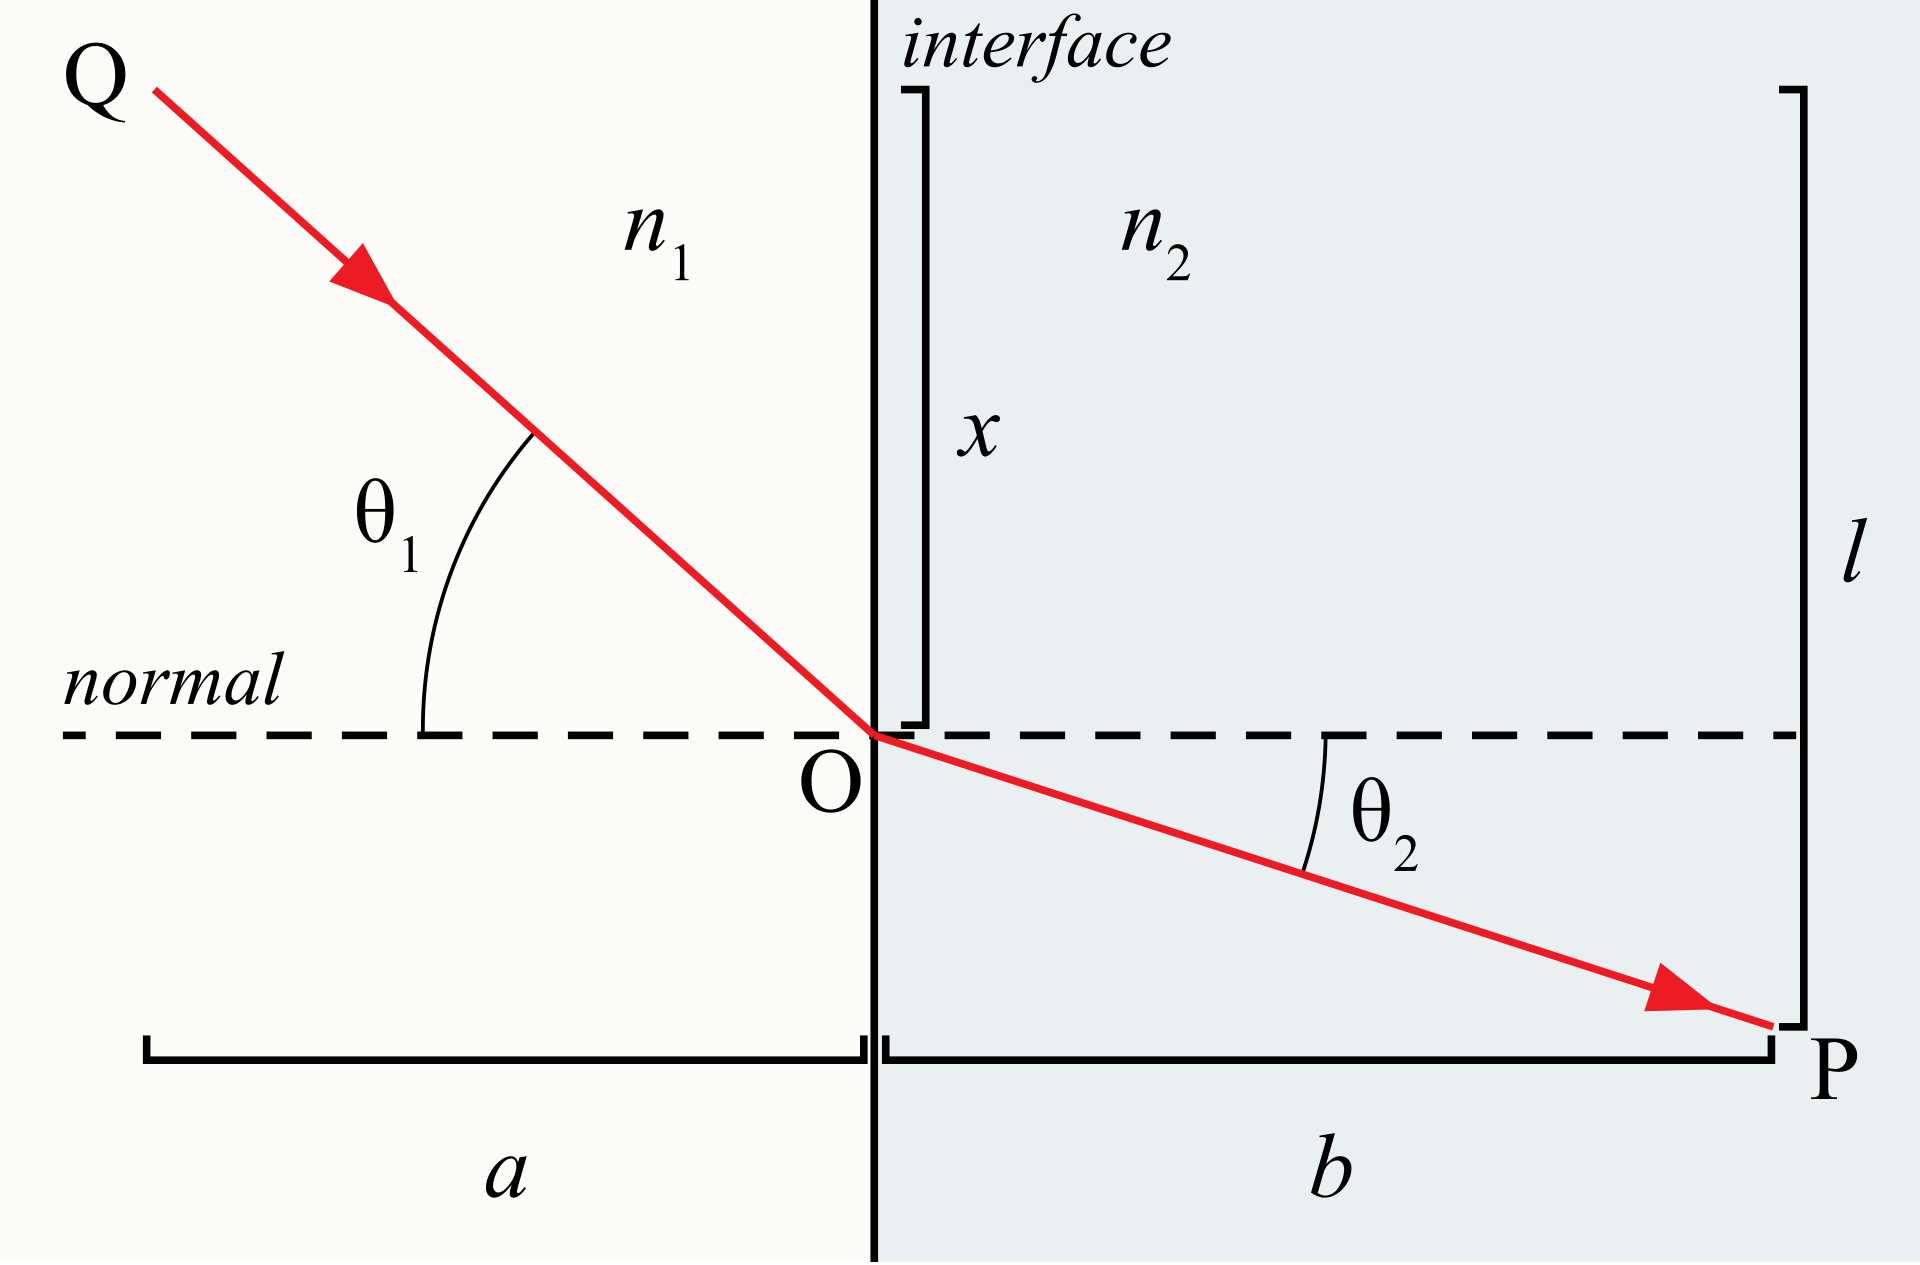
\includegraphics[scale=0.1]{notes/images/Snells-Law.JPG}
    \caption{Snell's Law Diagram}
\end{figure}
\FloatBarrier

We will now consider a special case of refraction, known as \textbf{total internal reflection} (TIR) of light at the boundary of two different media. The following conditions must be met in order for TIR to occur
\begin{itemize}
    \item Light must be travelling in a medium that has a higher refractive index than the boundary medium.
    \item The angle of incidence must be greater than the \textbf{critical angle} denoted $C$. The critical angle is dependent on the refractive indices of the media.
    \begin{figure}[h!]
        \centering
        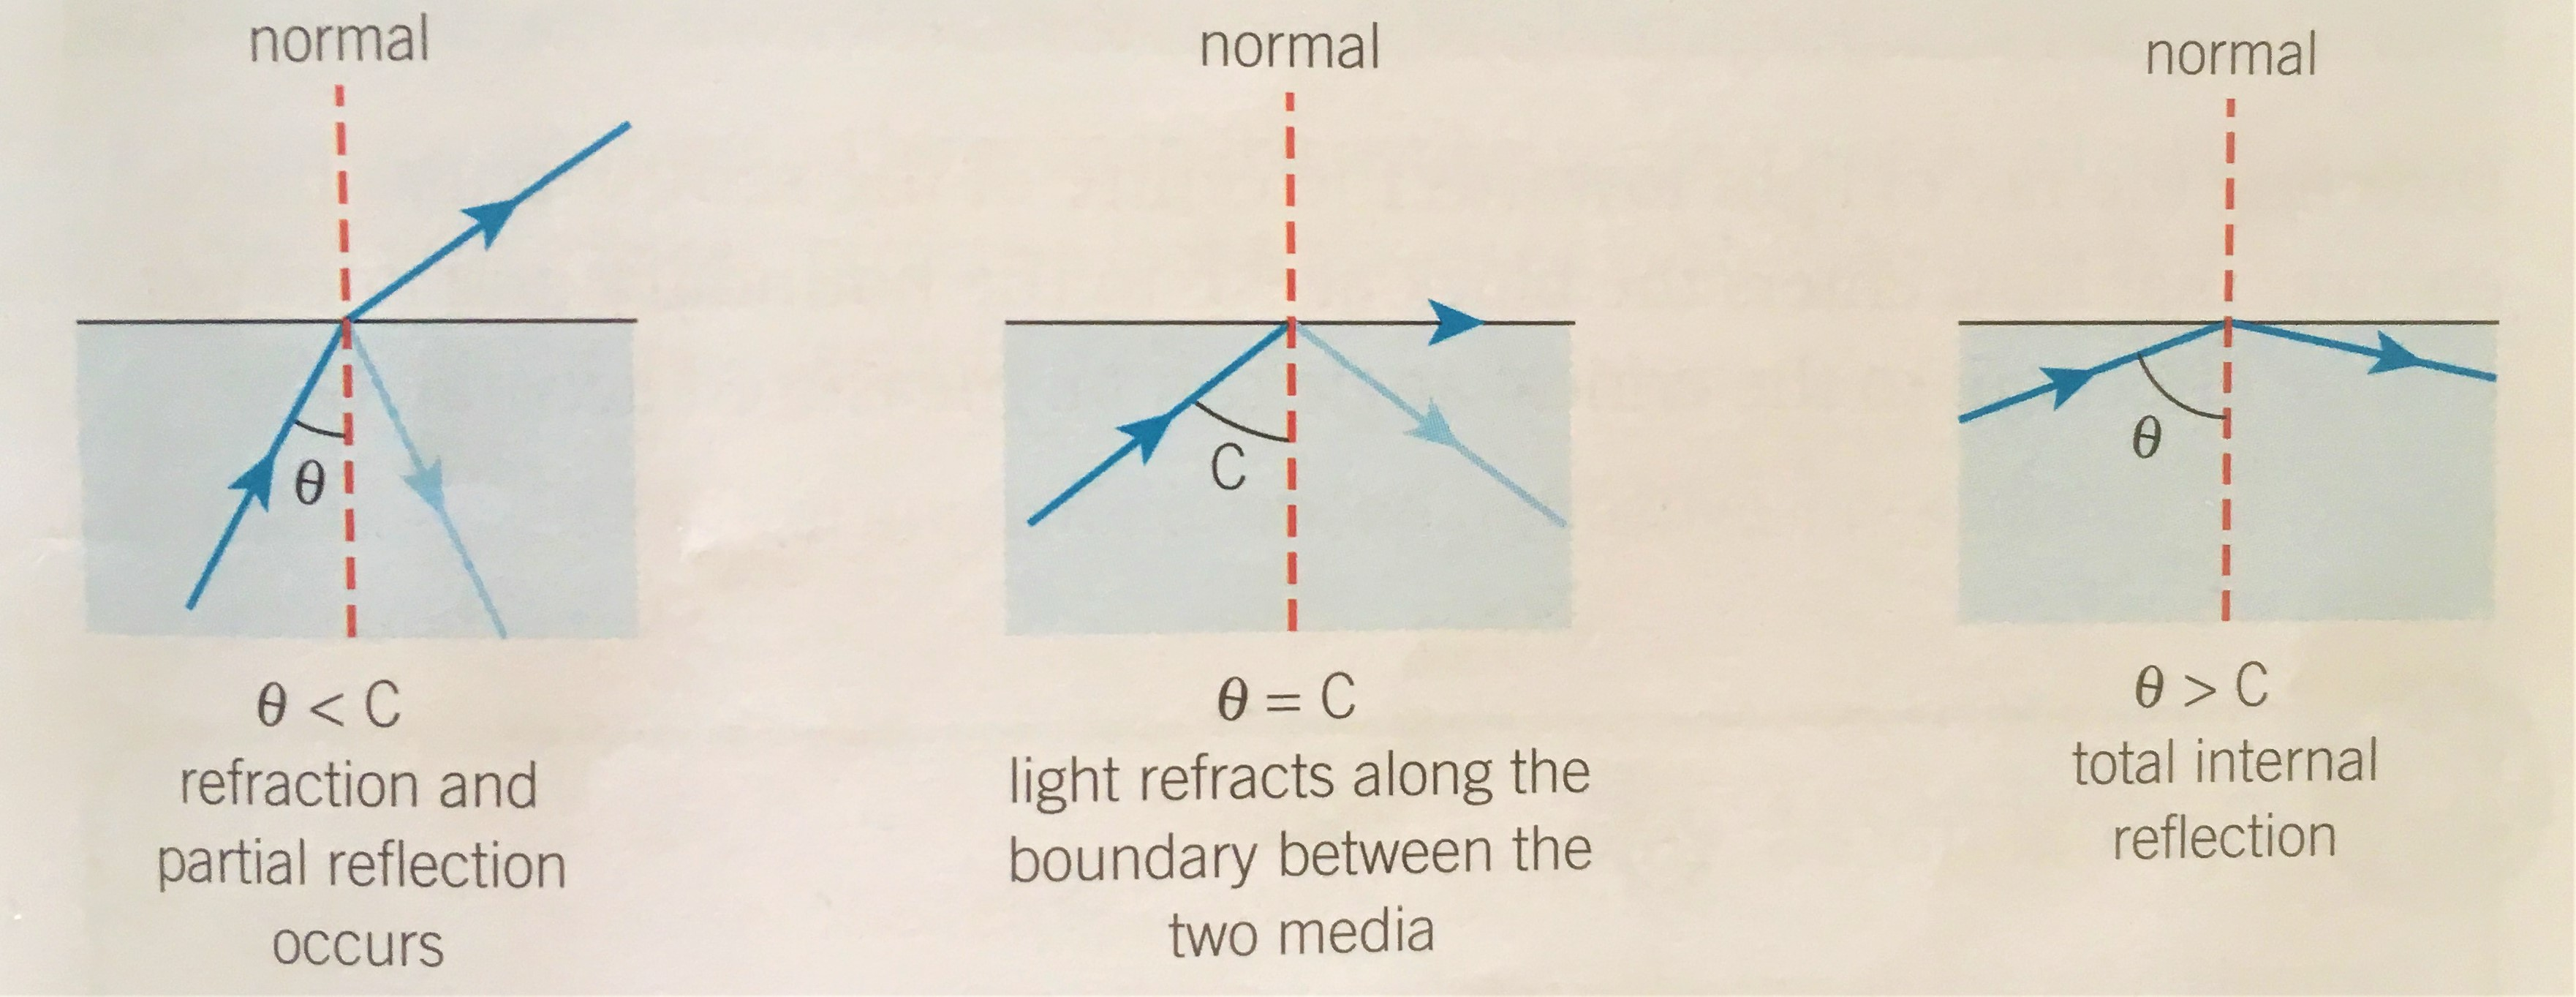
\includegraphics[scale=0.1]{notes/images/Critical-Angle.JPG}
    \end{figure}
    \FloatBarrier
    From Snell's law is follows that $n_1 \sin \theta_1 = n_2 \sin \theta_2$. Given $\theta_2 = \pi / 2$, we have $n_1 \sin C = n_2$, which yields:
    \begin{equation}
        \sin C = \frac{n_2}{n_1} = \frac{v_1}{v_2} = \frac{\lambda_1}{\lambda_2}. 
    \end{equation}
\end{itemize}



\subsection{Interference Patterns of Light}

Consider two waves. At certain points these superposed waves are in phase, interfering constructively, or out of phase, causing destructive interference. Most waves do not form a \textit{stable} interference pattern but one that changes all the time. In order to form a stable interference pattern, the incident waves must be \textbf{coherent}. This means that the waves from the sources must maintain a constant phase relation. For example, if two waves are in anti-phase, that is $\phi = \pi$, then this phase difference must not change with time to achieve a constant phase relation. 

Interference patterns contain a series of \textbf{minima} and \textbf{maxima}, where constructive and destructive interference occurs, respectively. Minima and maxima are a result of the two waves having travelled difference distances from their sources. This difference in the distance travelled is called the \textbf{path difference}, we will analyze these path differences mathematically to find criteria for the minima and maxima. 

Let us points $S_1$ and $S_2$ which serve as the sources of coherent waves. The waves emerging from the two sources then interfere and form an interference pattern. The points of maximum intensity correspond to maxima, and the converse is true for minima. Figure \ref{fig:interference-at-points} shows the ways in which the waves could combine to interfere constructively or destructively. 

\begin{figure}[h!]
    \centering
    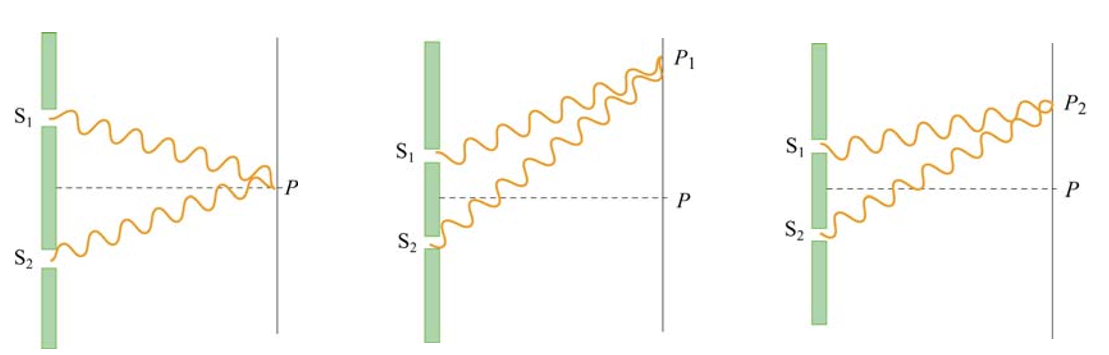
\includegraphics[scale=0.5]{notes/images/Interference-Two-Source-1.JPG}
    \caption{Constructive interference at $P$ and $P_1$. Destructive interference at $P_2$}
    \label{fig:interference-at-points}
\end{figure}
\FloatBarrier

The geometry of this interference pattern is shown below

\begin{figure}[h!]
    \centering
    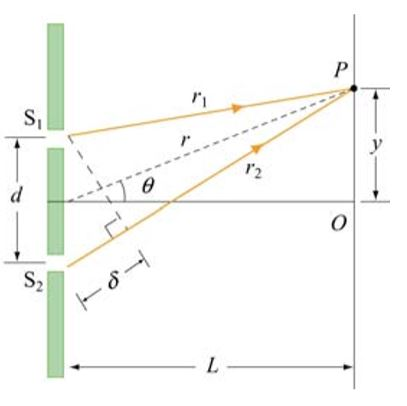
\includegraphics[scale=0.6]{notes/images/Interference-Two-Source-2.JPG}
    \caption{Two source experiment}
\end{figure}
\FloatBarrier

Consider a point $P$ where the two waves interfere, with a distance $y$ from the point $O$ that lies on a line perpendicular to the distance $L$ from the two source system. The wave from source 2 will travel an extra distance of $\delta = r_2 - r_2$ to the point $P$ than the wave from source 1. This extra distance is the \textit{path difference}. From the figure above, we have, using the law of cosines, 
\begin{equation}
    \label{eq:derivation-interference-1}
    r_1^2 = r^2 + \left(\frac{d}{2}\right)^2 - dr\cos \left(\frac{\pi}{2} - \theta\right) = r^2 + \left(\frac{d}{2}\right)^2 -dr \sin \theta
\end{equation}
and
\begin{equation}
    \label{eq:derivation-interference-2}
    r_2^2 = r^2 + \left(\frac{d}{2}\right)^2 - dr\cos \left(\frac{\pi}{2} + \theta\right) = r^2 + \left(\frac{d}{2}\right)^2 -dr \sin \theta
\end{equation}
Subtracting equation \ref{eq:derivation-interference-1} from equation \ref{eq:derivation-interference-2} yields:
\begin{equation*}
    r_2^2 - r_2^2 = (r_2 + r_1)(r_2 - r_1) = 2dr \sin \theta 
\end{equation*}
In the limit of $L \gg d$ (i.e. the distance to the screen is much greater than the distance between the sources), the sum of $r_2$ and $r_2$ may be approximated by $r_1 + r_2 \approx 2r$, and the path difference becomes
\begin{equation*}
    \delta = r_2 - r_1 \approx d \sin \theta 
\end{equation*}
In this limit, the two waves $r_1$ and $r_2$ are essentially treated as being parallel, as shown below

\begin{figure}[h!]
    \centering
    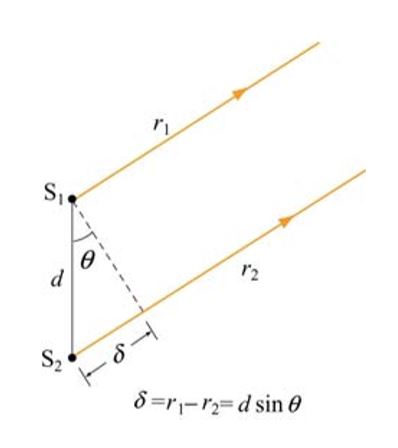
\includegraphics[scale=0.5]{notes/images/Interference-Two-Source-3.JPG}
    \caption{Path difference between the two waves, assuming $L \gg d$.}
\end{figure}
\FloatBarrier

Whether the two waves are in phase or out of phase is determined by the value of $\delta$. Constructive interference occurs when $\delta$ is zero or an integer multiple of the wave length $\lambda$:
\begin{equation}
    \label{eq:path-difference-constructive}
    \delta = d \sin \theta = n \lambda, \hspace{5mm} n = 0, \pm 1, \pm 2, \pm 3, \ldots
\end{equation}
where $n$ is called the \textit{order number}. The zeroth-order maximum corresponds to the central maxima, and the first-order maxima are the points of constructive interference either side of the central maxima, and so on.

On the other hand, when $\delta$ is equal to an odd integer multiple of $\lambda / 2$, the waves will be $\pi$ radians out of phase (i.e. anti-phase) at $P$, resulting in destructive interference. Hence the condition for destructive interference is given by
\begin{equation}
    \label{eq:path-difference-destructive}
    \delta = d \sin \theta = \left(n - \frac{1}{2}\right) \lambda, \hspace{5mm} n = \pm 1, \pm 2, \pm 3, \ldots
\end{equation}

In the figure below, we show how a path difference of $\lambda / 2$ results in a destructive interference and a path difference of $\lambda$ leads to constructive interference. 
\begin{figure}[h!]
    \centering
    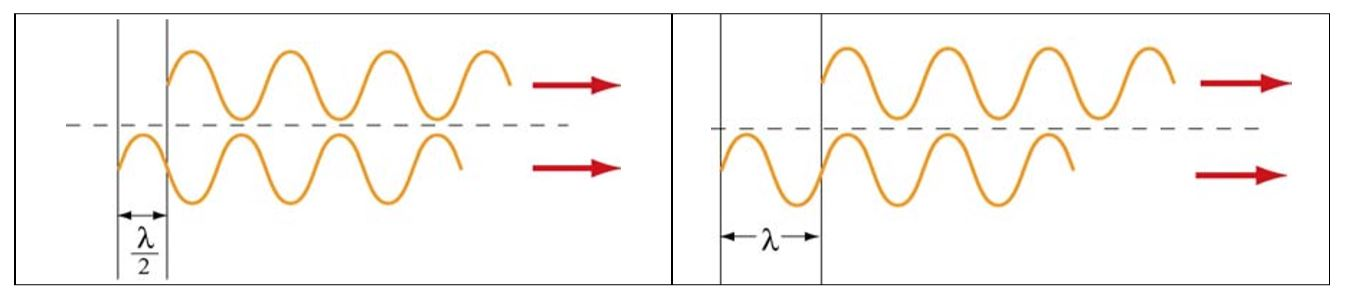
\includegraphics[scale=0.4]{notes/images/Interference-Two-Source-4.JPG}
    \caption{Destructive interference (left) and constructive interference (right).}
\end{figure}
\FloatBarrier
\noindent From the path difference, we can also deduce the phase difference between points on the waves using 
\begin{equation*}
    \phi = \frac{x}{\lambda} 2 \pi,
\end{equation*}
and substituting $\delta$ for $x$ in the equation above; yielding a phase difference for the central maxima of zero radians, $\pi$ radians for the first-order minima, $2\pi$ radians for the first-order maxima, $3\pi$ radians for the second-order minima, and so on.  The path differences and phase differences for a typical two source interference pattern are shown in the figure below

\begin{figure}[h!]
    \centering
    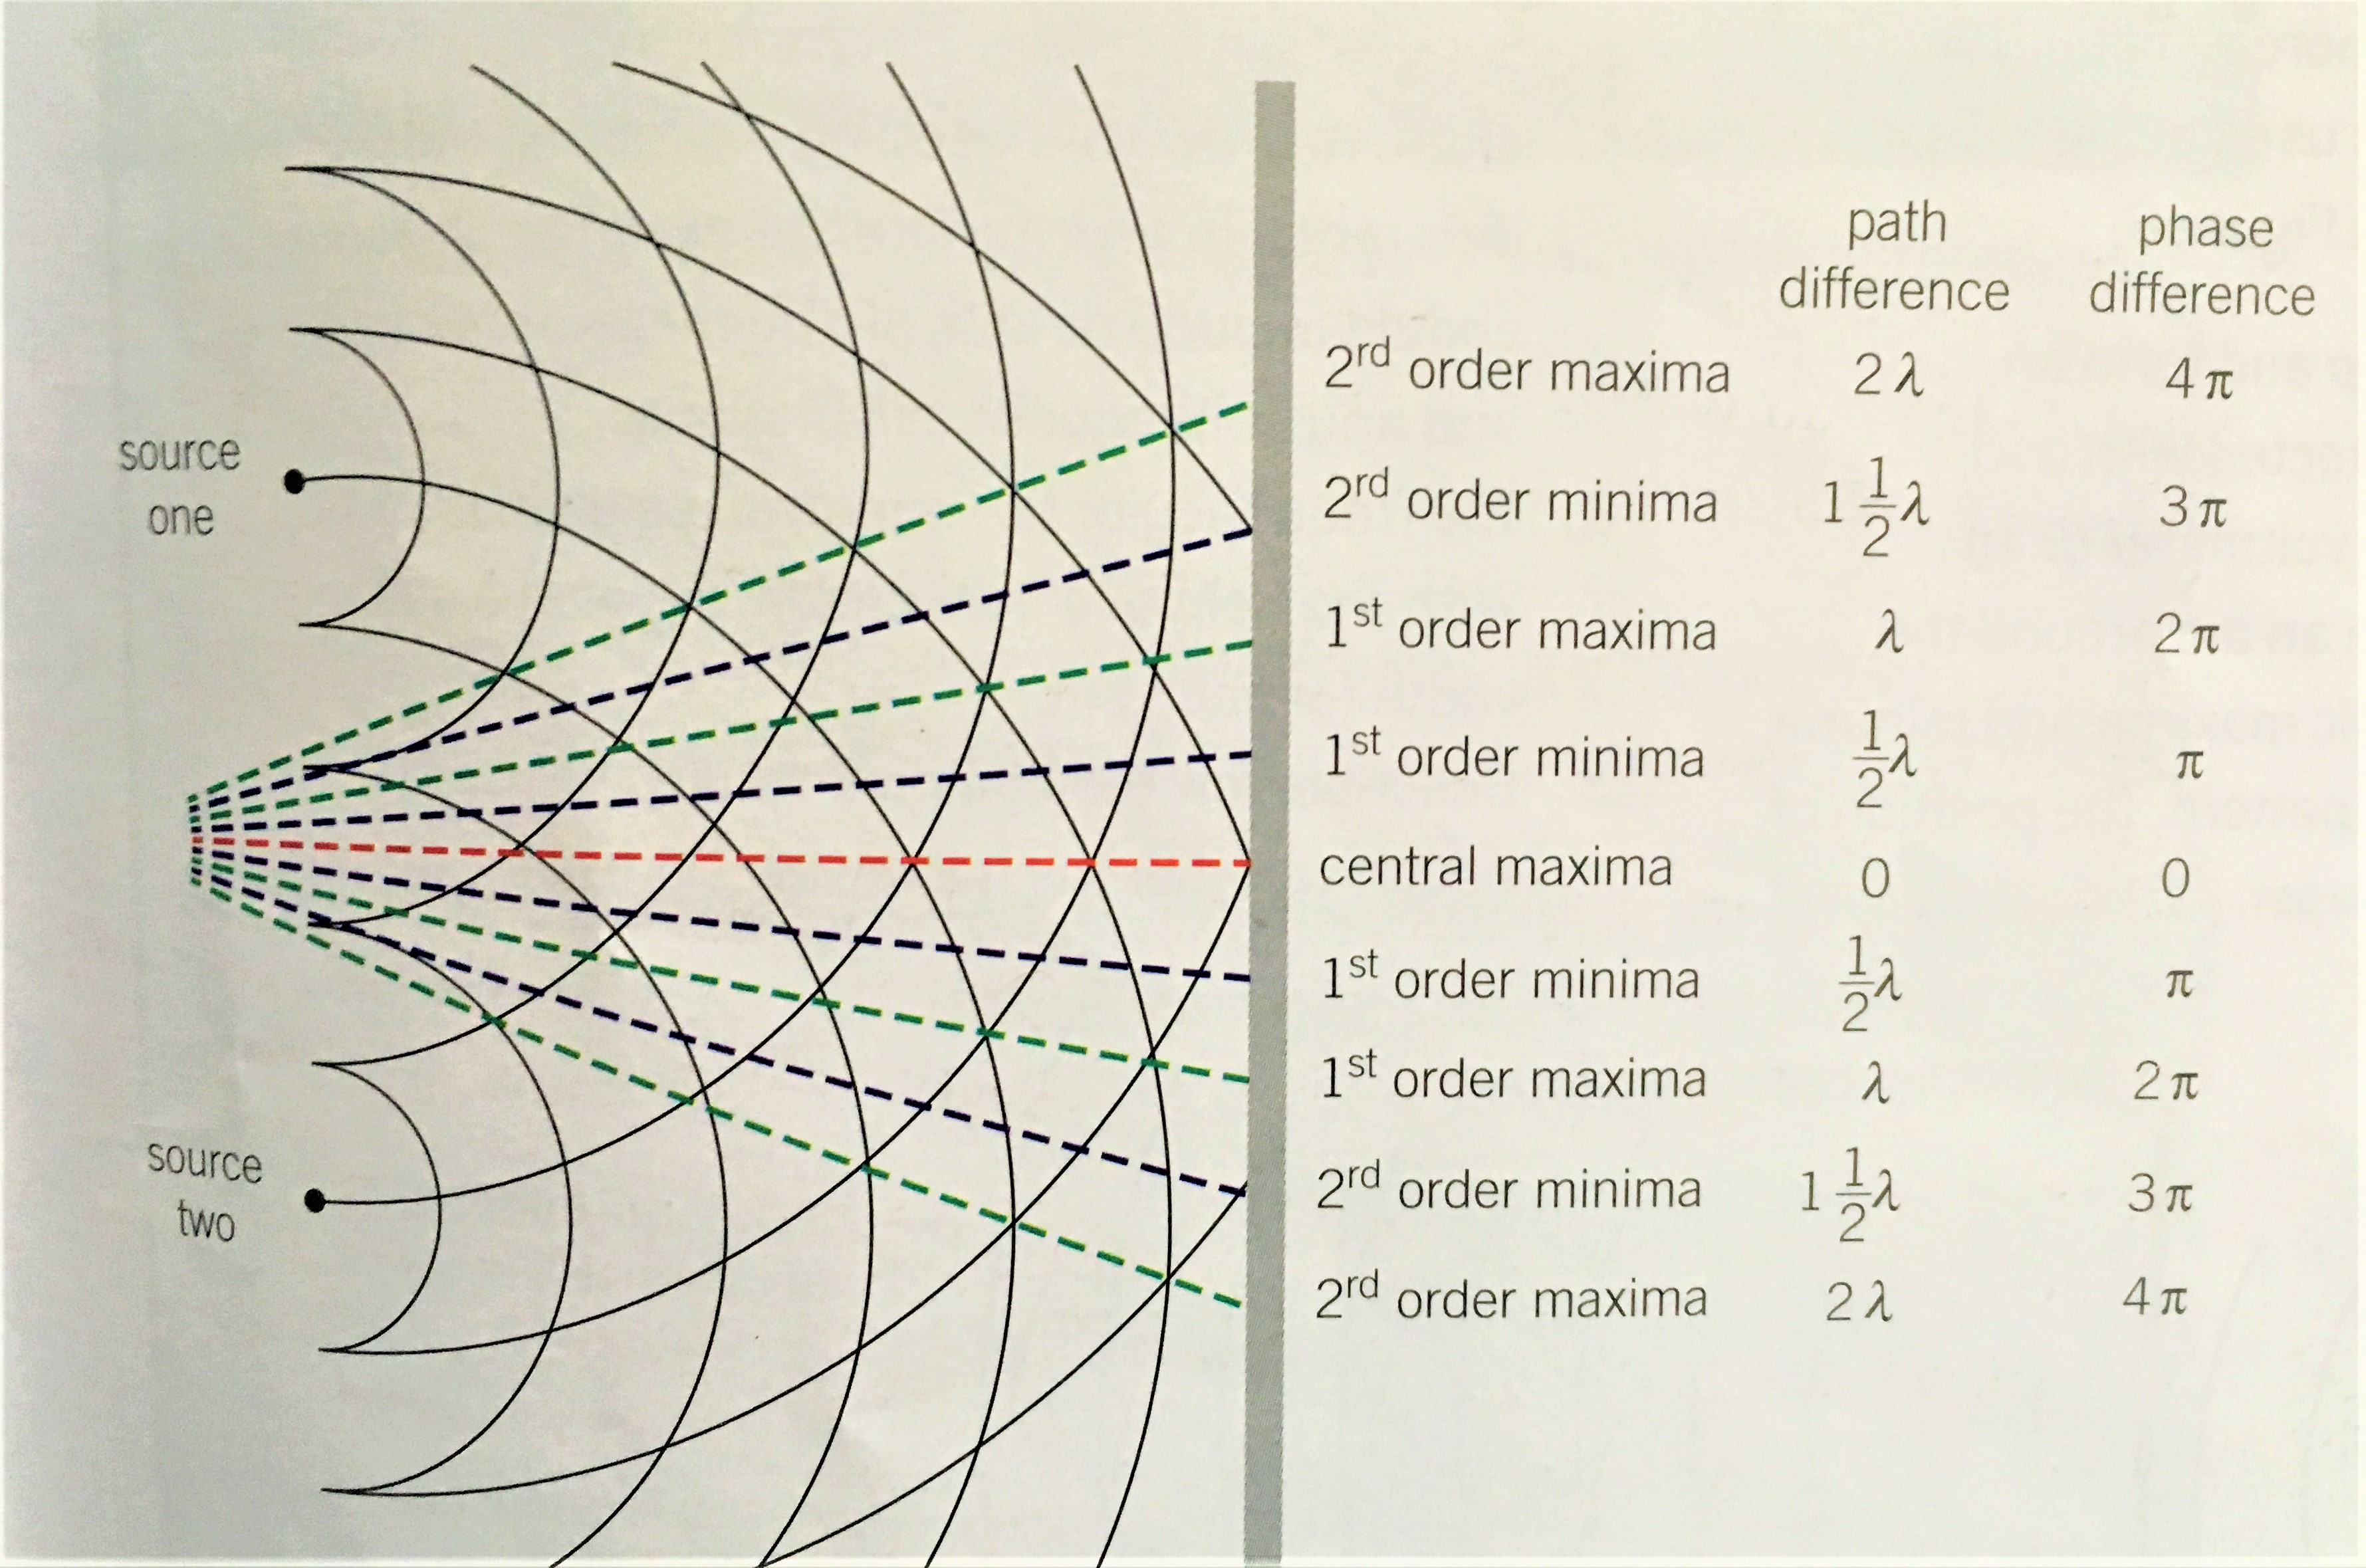
\includegraphics[scale=0.1]{notes/images/Interference.JPG}
    \caption{Two source wave interference pattern}
\end{figure}
\FloatBarrier

\subsection{Young's Double-Slit Experiment}

In 1801 Thomas Young carried out an experiment in which the wave nature of light was demonstrated. Two coherent waves are needed to form an interference pattern (as discussed above), Young devised a method to achieve this that now bears his name. He used a \textbf{monochromatic} source of light (which can be achieved by using a colour filter that allows only a specific frequency of light to pass) and a narrow single slit $S_0$ to diffract the light. The emerging light then arrives at the second screen which has two parallel slits $S_1$ and $S_2$ in phase. The two slits then serve as the sources of coherent light, with the emerging light waves interfering with each other to form an interference pattern on the viewing screen, The bright bands (fringes) correspond to maxima and the dark bands are minima; as shown below.
\begin{figure}[h!]
    \centering
    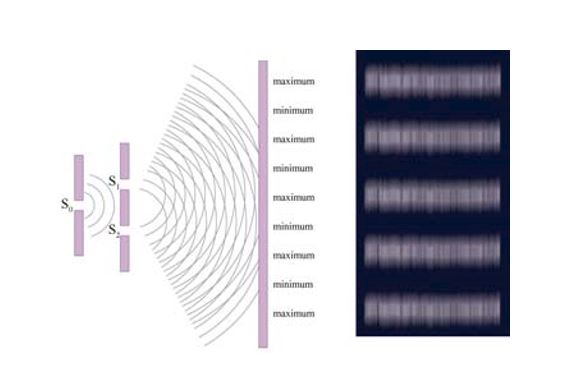
\includegraphics[scale=0.7]{notes/images/Interference-Single-Source-1.JPG}
    \caption{Young's double-slit experiment.}
\end{figure}
\FloatBarrier

The geometry of the double-slit interference experiment is shown below.
\begin{figure}[h!]
    \centering
    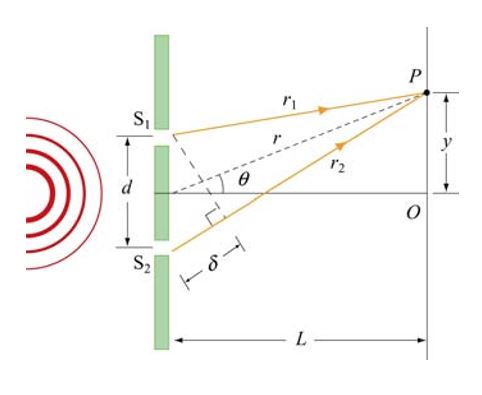
\includegraphics[scale=0.6]{notes/images/Interference-Single-Source-2.JPG}
    \caption{Double-slit experiment.}
\end{figure}
\FloatBarrier

Note that the problem is essentially identical to the two source interference experiment. To locate the positions of the fringes as measured vertically from the central point $O$, in addition to $L \gg d$, we shall also assume that the distance between the slits is much greater than the wavelength of the monochromatic light, $d \gg \lambda$. The conditions imply that the angle $\theta$ is very small, so we can apply the small angle approximations;
\begin{equation*}
    \sin \theta = \tan \theta = \frac{y}{L}
\end{equation*}

Substituting the above expression into the constructive and destructive interference conditions given in equations \ref{eq:path-difference-constructive} and \ref{eq:path-difference-destructive}, the positions of the bright and dark fringes are respectively,
\begin{equation}
    y_b = n \frac{\lambda L}{d}
\end{equation}
and
\begin{equation}
    y_d = \left(n - \frac{1}{2}\right) \frac{\lambda L}{d}.
\end{equation}
If we now consider the separation between two adjacent bright fringes $\Delta y$, we find that
\begin{equation*}
    \Delta y = \frac{\lambda L}{d},
\end{equation*}
which can be rearranged to solve for $\lambda$;
\begin{equation}
    \lambda = \frac{d \Delta y}{L}.
\end{equation}
Which is more commonly written as
\begin{equation}
    \lambda = \frac{ax}{D},
\end{equation}
where $x$ denotes the separation between two adjacent bright fringes (or two adjacent dark fringes), $a$ denotes the separation between the two slits and $D$ denotes the separation between the slits and the screen.
    \clearpage
    
    \chapter{Electricity}
    \section{Electric Fields}

\subsection{Charge and Electric Force}

Charge is the fundamental quantity of electricity, and therefore cannot be defined. However, we can study how charges interacts. Electric charge comes in two and only two types, \textbf{positive} ($+$) and \textbf{negative} ($-$), carried by protons and electrons respectively; although the definition of which is completely arbitrary, as there doesn't exist an objective test that can be used to distinguish positive charge from negative charge, the sign of a charge can only be determined by comparison to a charge with a charge whose sign is already known. Note that the term neutral does not refer to a third type of charge, but to the presence in a region of positive and negative charges in equal amount. 

The law that governs how charged particles interact is Coulomb's Law which states: the magnitude force between two particles with charges $q_1$ and $q_2$ has the following relationship
\begin{equation}
    \| \vec{F} \| \propto \frac{q_1 q_2}{r^2},
\end{equation}
where $r$ is the distance between the centres of the particles. We measure a constant of proportionality as $k_e$, the so-called electrostatic constant. Alternatively we sometimes write the electrostatic constant in terms of vacuum permittivity $\varepsilon_0$. such that $k_e = \frac{1}{4\pi \varepsilon_0}$. 

More formally. We say the electric force $\vec{F}_{1,2}$ exerted on particle 1 due to particle 2 with charges $q_1$ and $q_2$ and position vectors $\vec{r}_1$ and $\vec{r}_2$ respectively is given by
\begin{equation}
    \label{eq:coulombs-law}
    \vec{F}_{1,2} = \frac{q_1 q_2}{4 \pi \varepsilon_0 \| r_{2,1} \|^2} \hat{r}_{2,1},
\end{equation}
where $\hat{r}_{2,1}$ is the unit separation vector pointing from particle 2 to particle 1, so we have
\begin{equation}
    \hat{r}_{2,1} = \frac{\vec{r}_{2,1}}{\| \vec{r}_{2,1}\|} \text{ and } \vec{r}_{2,1} = \vec{r}_1 - \vec{r}_2.
\end{equation}
It also follows that from Newton's third law of motion, the force on the particle with charge $q_2$ exerted by $q_1$ is given by
\begin{equation}
    \vec{F}_{2, 1} = - \vec{F}_{1, 2}.
\end{equation}
The rule of action is implied by Coulomb's Law, however, it is so fundamental that it deserves to be a law in it's own right.
\begin{theorem}{(\textbf{Rule of Action})}
\textit{The rule of action states that like charges repel and opposite charges attract.}
\end{theorem}
Electric charge is also a conserved property; the net charge (see definition \ref{def:net-charge}) of an isolated system cannot change.
\begin{definition}{(\textbf{Net Charge})}
\label{def:net-charge}
\textit{The net charge of an isolated system, $Q_{net}$, is defined as the sum of positive charges, $Q^{+}$, minus the sum of negative charges, $Q^{-}$.}
\begin{equation}
    Q_{net} = Q^{+} - Q^{-}
\end{equation}
\end{definition}

Charge is also quantized, it comes in integer multiples of individual small units called the \textbf{elementary charge}, $e$, about $1.6 \times 10^{-19}$ coulombs, which is the smallest charge which can exist (excluding quarks, see section ??). The proton has a charge of $+e$ and the electron has a charge of $-e$. The unit of electric charge is the coulomb $(C)$. Due to this property, we can the net charge of an isolated system $Q_{net}$ is,
\begin{equation}
    Q_{net} = \eta e
\end{equation}
where $\eta$ is the number of charge carriers in the system, where $\eta \in \mathbb{Z}$.

\subsection{The Electric Field}

While we need two charges to quantify the electric force, we denote the \textbf{electric field} for any single charge distribution to describe it's effect on other charges. In classical field theory, we say a charge in space produces an electric field $\vec{E}$ with spherical symmetry. We have 
\begin{equation}
    \vec{E} = \frac{q_1}{4 \pi \varepsilon_0 \| \vec{r} \|^2} \hat{r}
\end{equation}
and so we have
\begin{equation}
    \vec{E} = \frac{\vec{F}}{q_2}
\end{equation}
where $\hat{r}$ is a unit surface vector, that is $\vec{r}$ is a vector that is always perpendicular to the surface of the charge. So $\vec{r}$ is always pointing away from the charge (and towards other charges). In advanced Physics an electric field is represented as a vector field (as shown below), however, in A2 Physics we use \textit{field lines} to represent the electric field, also shown below. 
\begin{figure}[h!]
    \centering
    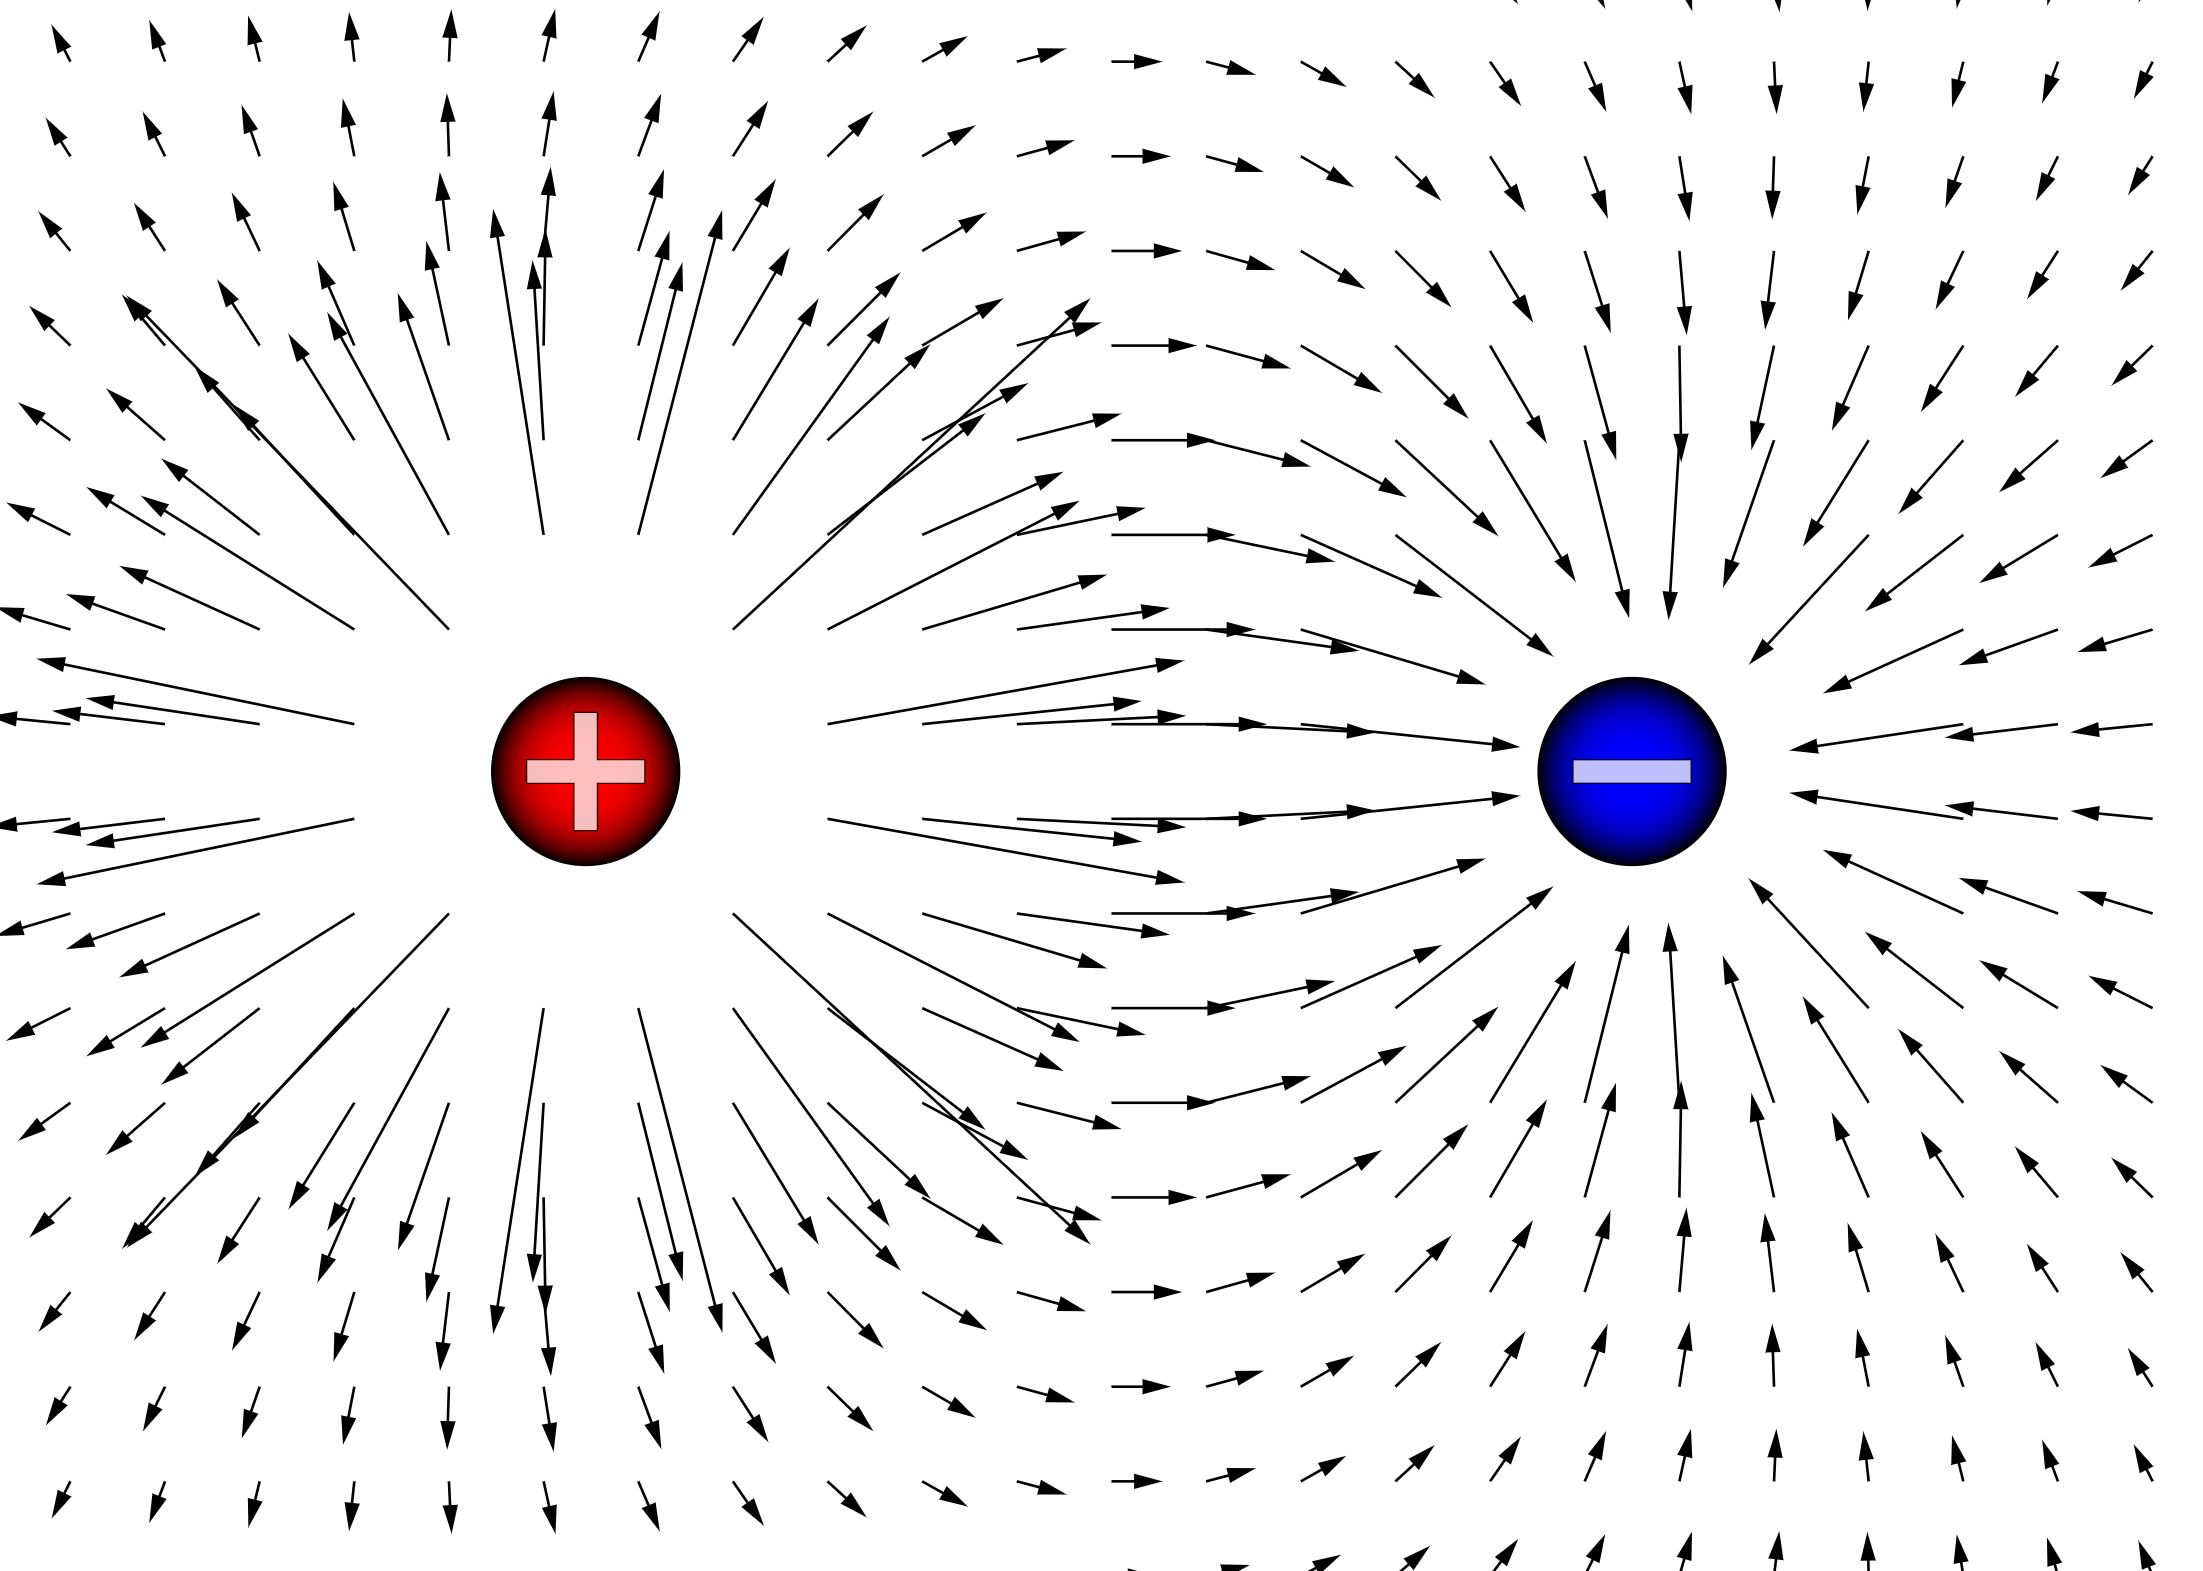
\includegraphics[scale=0.25]{notes/images/Electric-Field-Vector.JPG}
    \caption{Electric field as a vector field}
\end{figure}
\FloatBarrier

\begin{figure}[h!]
    \centering
    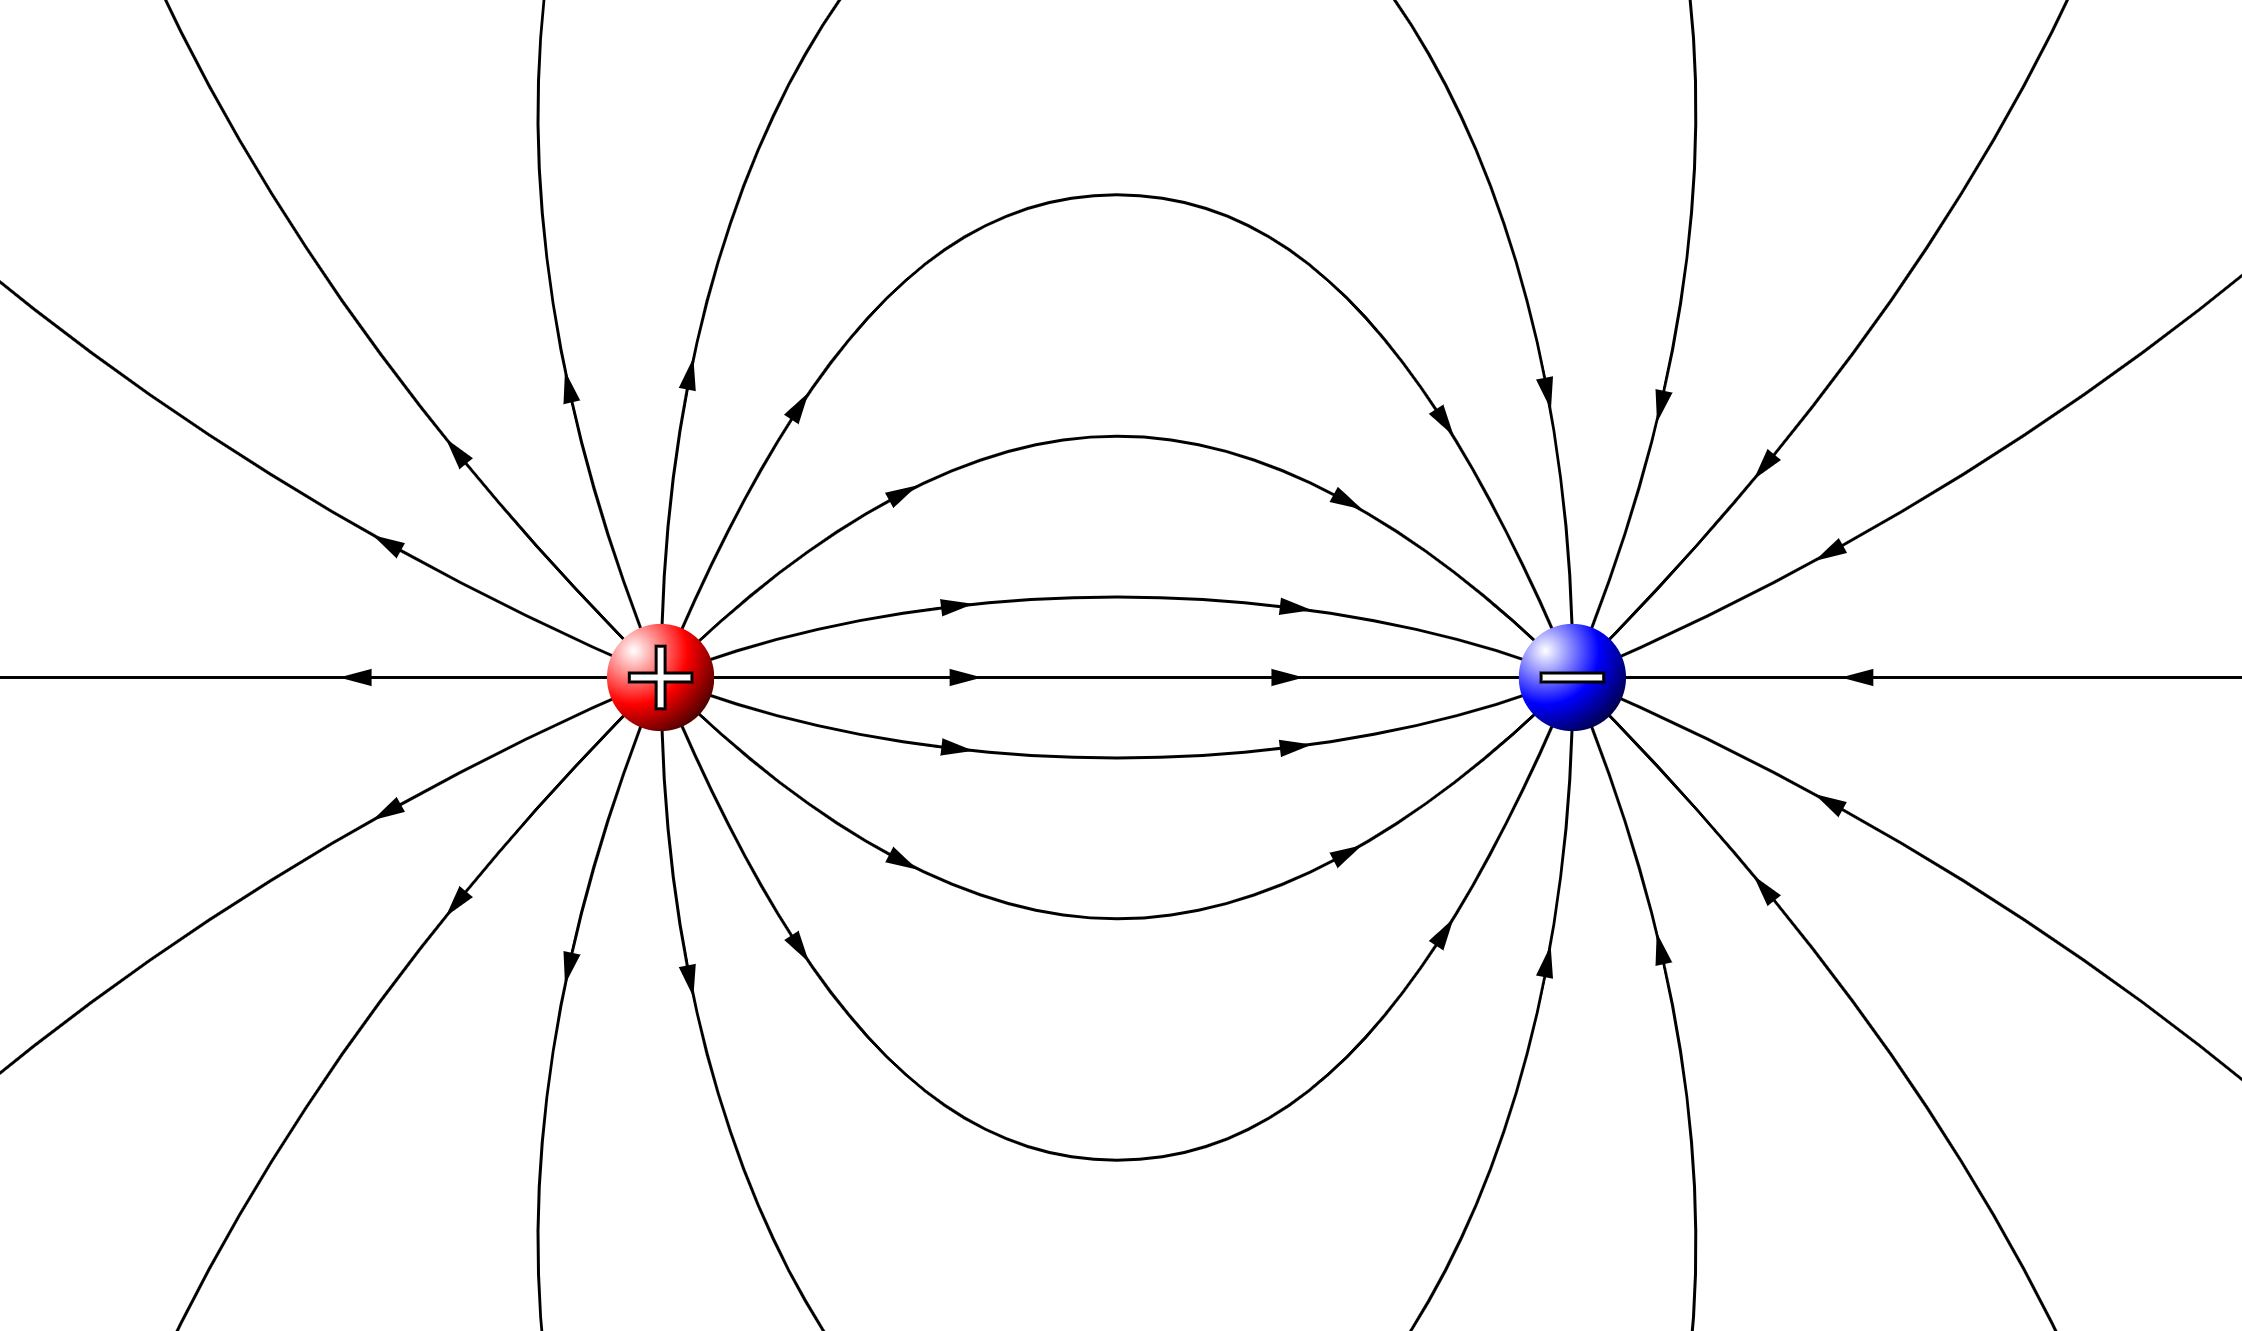
\includegraphics[scale=0.25]{notes/images/Electric-Field-Lines.JPG}
    \caption{Electric field as field lines}
\end{figure}
\FloatBarrier

The magnitude of the electric field is commonly known as the \textbf{electric field strength} and is denoted by the euclidean length of the electric field $\vec{E}$ ($\| \vec{E} \|$). 


\subsection{Potential Energy}

In general for a field, the potential $E_p$ is defined by considering the negative work done moving a charged particle from position 1 to 2, that is
\begin{equation}
    \Delta E_p = -W = - \int_C \vec{F} \cdot \mathop{\mathrm{d}\vec{s}}.
\end{equation}
Using the relations from \ref{eq:work-done-variable-force-vector} and \ref{eq:coulombs-law}, we obtain

\begin{align}
     \Delta E_p &= - \int_C k_e \frac{q_1 q_2}{\| \vec{r} \|^2} \hat{r} \cdot \mathop{\mathrm{d}\vec{s}} \\
    &= - k_e q_1 q_2 \int_C \frac{\vec{r}}{\| \vec{r} \|^3} \cdot \mathop{\mathrm{d}\vec{s}}.
\end{align}
Since $\vec{r}$ is parallel to $\mathop{\mathrm{d}\vec{s}}$, we do not need to consider a tangential vector to the curve $C$. So we have,
\begin{align}
    \Delta E_p &= - k_e q_1 q_2 \int_{r_1}^{r_2} \frac{1}{s^2} \mathop{\mathrm{d}s} \\
    &= k_e q_1 q_2 \left(\frac{1}{r_2} - \frac{1}{r_1}\right).
\end{align}

This result is generally true for both 2 and 3 dimension motion of charges. We note that it is the \textit{difference} in potential energy that is important. So we have a reference point at $r = \infty$ such that $E_p (r) = 0$. So we have
\begin{align}
    E_{p}(\infty) - E_p (r) &= - k_e q_1 q_2 \frac{1}{r} \\ 
    E_p (r) &= k_e \frac{q_1 q_2}{r}.
\end{align}

\subsection{Electric Potential}

In general for a field, the potential $V$ is defined as 
\begin{equation}
    V = \frac{E_p}{q_2},
\end{equation}
where $q_1$ is a fixed charged and $q_2$ is our so-called \textit{test charge}. So for a single point charge, the potential at a point with distance $r$ from the point charge is given by
\begin{equation}
    V = k_e \frac{q_1}{r} = \| \vec{E} \|r
\end{equation}
Recall the definition of an electric field $\vec{F} = q_2 \vec{E}$, so 
\begin{align}
    \label{eq:change-in-potential}
    \Delta V &= - \frac{1}{q_2} \int_C \vec{F} \cdot \mathop{\mathrm{d}\vec{s}} \\
    &= - \int_C \vec{E} \cdot \mathop{\mathrm{d}\vec{s}}
\end{align}
The \textbf{potential difference} is then defined (in the context of a field) as the rate of work done per unit of charge between two points around the particle of charge $q_1$. We won't evaluate this line integral in general. However, we will consider a specific case, a uniform electric field. 

Consider a path going from the $-ve$ plate to the $+ve$ plate and the potential at the point $P$, denoted $V_P$ (See figure \ref{fig:uniform-field-derivation}). 

\begin{figure}[h!]
    \centering
    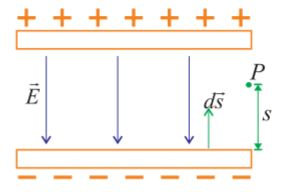
\includegraphics{notes/images/Uniform-Field-Derivation.JPG}
    \caption{A uniform field}
    \label{fig:uniform-field-derivation}
\end{figure}
\FloatBarrier

From the integral above, we'll define our initial position (at the $-ve$ plate) to have a potential of zero volts. From this we have
\begin{equation}
    \Delta V = V_p - V_{-ve} = - \int_0^s  \vec{E} \cdot \mathop{\mathrm{d}\vec{s}}. 
\end{equation}
Since $\hat{E} = -\mathop{\mathrm{d}\hat{s}}$, from this we obtain, 
\begin{align}
    V_p &= - \int_0^s (- \| \vec{E} \| ) \mathop{\mathrm{d}s} \\
    &= \| \vec{E} \| \int_0^s \mathop{\mathrm{d}s} \\
    &= \| \vec{E} \| s.    
\end{align}

Despite not evaluating the line integral above (in the general case), we can make some intuitive guesses about how it may change with respect to small changes in distance from the single point charge. We can quickly see that there exists an infinite number of positions where the potential is constant. This is due to the inverse square law of the electric field strength. The positions form a ``surface'' known as an \textbf{Equipotential surface}. Formally, an equipotential surface is a surface on which the \textit{potential is constant}. 

Having defined the concept of equipotential surfaces, we can now consider some of their properties. We note that a charge can move freely on an equipotential surface without any work done and the electric field lines must be perpendicular to the equipotential surfaces (see figure \ref{fig:equipotential}) this is because an equipotential surface has a constant potential, so the change in potential $\Delta V$ is zero. So $\vec{E} \cdot \mathop{\mathrm{d}\vec{s}} = 0$, where $\mathop{\mathrm{d}\vec{s}}$ is tangent to the equipotential surface, it follows from the definition of the dot product that $\vec{E}$ must be perpendicular to $\mathop{\mathrm{d}\vec{s}}$ and therefore perpendicular to the equipotential surface.    

\begin{figure}[h!]
    \centering
    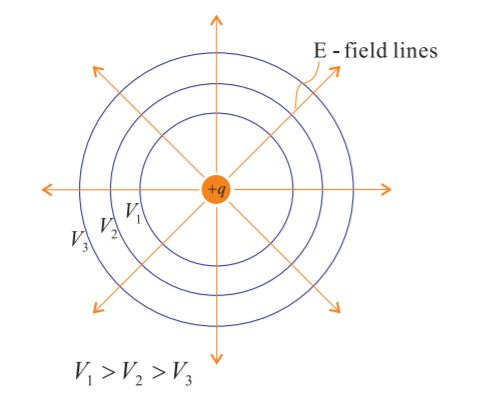
\includegraphics{notes/images/Equipotential.JPG}
    \caption{Equipotential surfaces of a point charge}
    \label{fig:equipotential}
\end{figure}
\FloatBarrier


\section{Circuits}

\subsection{Current}

\begin{definition}{(\textbf{Current})}
\label{def:current}
\textit{An electric current $I$ is defined as the rate at which charge flows through a surface (the cross section of a wire, for example).} 
\begin{equation}
    I = \frac{\mathop{\mathrm{d}Q}}{\mathop{\mathrm{d}t}}
\end{equation}
\textit{measured in \textbf{amperes} (A).}
\end{definition}

Since charge is measured in coulombs and time is measured in seconds, an ampere is the same as a coulomb per second.
\begin{equation*}
    \left[A\right] = \left[Cs^{-1}\right]
\end{equation*}
Note that this is not a definition. The ampere is a fundamental unit in the International System. Fundamental units are themselves defined by experiment. In the case of the ampere, the experiment is electromagnetic in nature. We also note, for completeness, 
\begin{equation}
    Q = \int_{t_1}^{t_2} I \mathop{\mathrm{d}t},
\end{equation}
which reduces to $Q = It$ for constant current.

\subsection{Moving Charges}

An electric current usually flows through a conductor (i.e. metals). Metals are bonded metallically, which produces \textit{delocalized} electrons which can flow freely. An electric current is created in a conductor when one end of the conductor is positive and the other is negative, it follows from the rule of action that electrons will flow to the positive end of the conductor.

\subsubsection{Conventional current}

Conventional current assumes that current flows out of the positive terminal, however, by the rule of action we know that charge carriers flow from the negative terminal to the positive terminal of the power supply.

\begin{figure}[h!]
    \centering
    \begin{circuitikz}
        \draw (0,0) to [battery](0,4) to [ammeter](4,4) -- (4,0) to [lamp](0,0);
        \draw[-latex] (4,-1) -- (0,-1);
        \node at (2, -1.5) {$\textit{electron flow}$};
        \draw[-latex] (0,-2) -- (4,-2);
        \node at (2, -2.5) {$\textit{conventional current}$};
    \end{circuitikz}
    \caption{Simple circuit with electron flow and conventional current.}
    \label{fig:conventional-current}
\end{figure}
\FloatBarrier

Although conventional current is incorrect, it makes no difference which way current is flowing as long as it is used \textit{consistently}. 

\subsection{Kirchhoff's First Law}

Kirchhoff's circuits laws are two equalities that deal with the current and potential difference (see section \ref{subsection:potential-difference}), first described by German physicist Gustav Kirchhoff. In this section, we shall discuss Kirchhoff's first law, sometimes referred to as \textbf{kirchhoff's current law}.

\begin{theorem}{(\textbf{Kirchhoff's first law})}
\textit{Kirchhoff's first law states that for any point in an electrical circuit, the sum of currents entering a given point is equal to the sum of currents leaving that point. }
\begin{equation}
    \sum I_{in} = \sum I_{out}
\end{equation}
\end{theorem}

Kirchhoff's first law can be seen as a corollary of the conservation of charge, it follows that if charge in an isolated system is constant and current is defined as the rate of which charge flows across a surface then current in an isolated system is constant, since neither charge nor time can be destroyed.

\subsection{Mean Drift Velocity}

As electrons move in a wire, they collide with positive metal ions; it follows that electrons do not have a constant velocity and not every electron has the same velocity. Hence we must consider the average, or \textit{mean}, velocity of the electrons in the wire. Although it is evident that the mean drift velocity is dependent on physical characteristics of the conductor.

\subsubsection{Classification of conductors}

A material can be classified using it's number density $n$, the number of free electrons per unit of volume, measured in $m^{-3}$. It also follows from the definition of number density that
\begin{equation*}
    n \propto \text{conductivity}.
\end{equation*}
Thus we can use number density to classify materials into conductors, semi conductors and insulators. 

\begin{table}[h!]
    \centering
    \resizebox{.6\textwidth}{!}{
    \begin{tabular}{c|c}
        \textit{Material type} & \textit{Approx. number density} ($m^{-3}$) \\
        \hline
        \textit{Conductor} & $10^{28}$ \\
        \textit{Semi-conductor} & $10^{17}$
    \end{tabular}
    }
\end{table}
\FloatBarrier

\begin{theorem}
\textit{The electric current $I$ in a conductor with cross sectional area $A$, number density $n$ and mean drift velocity of charge carriers $\overline{\vec{v}}$ is given by}
\begin{equation}
    I = Ane\|\vec{v}\|,
\end{equation}
\textit{where e is the elementary charge.}

\begin{proof}
\textit{Consider a conductor with volume $V$ $m^3$ and number density $n$ $m^{-3}$. It follows from the definition of number density and qunatization of charge that}
\begin{equation*}
    Q = neV.
\end{equation*}
\textit{Applying this to the definition of electric current, we have}
\begin{equation*}
    I = \frac{neV}{\mathop{\Delta t}}.
\end{equation*}
\textit{When there is an electric current, a certain volume of charge carriers pass through a given point each second. This volume is dependent on the cross sectional area $A$ of the conductor and the mean drift velocity of the charge carriers, so}
\begin{equation*}
    \frac{V}{\Delta t} = A\|\vec{v}\|.
\end{equation*}
\textit{Then $I = Ane\|\vec{v}\|$, thus completing the proof.}
\end{proof}
\end{theorem}

\subsection{Potential Difference and Electromotive force}
\label{subsection:potential-difference}

\begin{definition}{(\textbf{Potential Difference})}
\textit{Potential difference $V$ is defined as the rate of energy transferred $W$ per unit of charge $Q$.}
\begin{equation}
    V = \frac{\mathop{\mathrm{d}W}}{\mathop{\mathrm{d}Q}}.
\end{equation}
\textit{Alternatively (without Calculus), we have}
\begin{equation}
    V = \frac{\Delta W}{Q},
\end{equation}
\textit{measured in \textbf{volts} (V).}
\end{definition}
Since energy is measured in joules and charge is measured in coulombs, a volt is the same as a joule per coulomb.
\begin{equation*}
    [V] = [JC^{-1}]
\end{equation*}






Potential difference is sometimes described as the work done \textit{by} charge carriers, whereas, Electromotive force (e.m.f) is used to describe work done \textit{on} the charge carriers, it follows from this that Electromotive force is used when charge carriers gain energy from a source.

\begin{definition}{(\textbf{Electromotive Force})}
\textit{Electromotive force $\varepsilon$ is defined as the rate of energy $W$ transferred to electrical energy per unit of charge $Q$.}
\begin{equation}
    \varepsilon = \frac{\mathop{\mathrm{d}W}}{\mathop{\mathrm{d}Q}}
\end{equation}
\textit{measured in \textbf{volts} (V).}
\end{definition}

\subsection{The Electron Gun}

An electron gun is a device used to produce a narrow beam of electrons. In this section we will discuss the method of operation and transfer of energy that occurs in the electron gun. In later sections, we will relate the method of operation to electric fields. 

\subsubsection{Method of Operation}

\begin{figure}[h!]
    \centering
    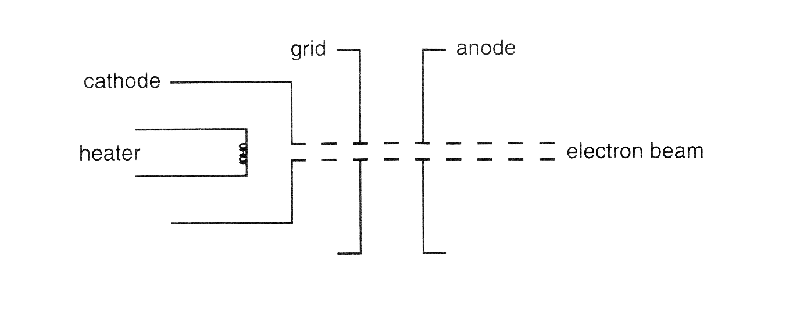
\includegraphics[scale=1.5]{notes/images/Electron-Gun.JPG}
    \caption{An Electron Gun}
\end{figure}
\FloatBarrier

\begin{enumerate}
    \item A small wire filament is heated via an electric current. The electrons in the filament gain kinetic energy ($E_k$). If the $E_k$ is large enough they escape the surface of the metal. This process is called \textit{thermionic emission} (the emission of electrons via heat). 
    \item A high potential difference (also known as the accelerating p.d) is applied to a cathode and an anode. The gun is placed in a vacuum, allowing free electrons to travel towards the anode, which is made positive with respect to the cathode, hence the electrons gain kinetic energy. 
    \item The anode has a small hole in it. So while some electrons hit the anode to return to the cell, others emerge through the hole in the anode with considerable speed.
\end{enumerate}

\subsubsection{Transfer of Energy in the Electron Gun}

The energy transferred to charges moving through a potential difference in a vacuum is transferred to the charges themselves as kinetic energy. From the definition of potential difference, the work done on a single electron travelling from the cathode to the anode is given by $eV$, where $e$ is the elementary charge and $V$ is the accelerating potential difference. 

By considering the law of conservation of energy, we can relate to the work done to the gain in kinetic energy, hence
\begin{align*}
    \text{Energy transferred to electron} &= eV \\
    &= E_k \\
    &= \frac{1}{2}m_e \| \vec{v} \|^2
\end{align*}
where $m_e$ is the mass of a single electron.

\subsubsection{Particle Accelerators}

An electron gun is a type of partial accelerator, we also have different types of particle accelerators such as \textit{linear particle accelerators} (LINACs). LINACs use a series of cylindrical electrodes (drift tubes) to accelerate subatomic particles such as electrons. The polarity off the drift tubes alternate when electrons leave the tubes thus attracting the electron to the next tube, allowing the electron to gain kinetic energy. Every time an electron moves from one tube to another it gains energy equal to $eV$. With a large number of electrodes, electrons can be accelerated to extremely high velocities. 

\subsection{Electrical Resistance}

\begin{definition}{(\textbf{Electrical Resistance})}
\textit{Electrical resistance is defined as the measure of the degree to which a conductor opposes the flow of charge carriers through that conductor,
measured in \textbf{ohms} ($\ohm$). Mathematically, the resistance R of an object is defined as the ratio of potential difference across it V to current through it I,}
\begin{equation}
    R = \frac{V}{I}
\end{equation}
\end{definition}

Since potential difference is measured in volts and current is measured in amperes, it follows that an ohm is the same as a volt per ampere.
\begin{equation*}
    [\ohm] = [VA^{-1}]
\end{equation*}

For a wide variety of materials and conditions, $V$ and $I$ are directly proportional to each other, and therefore $R$ is constant. This proportionality is called \textbf{Ohm's law}, and materials that satisfy it are called \textit{ohmic} materials.

\begin{theorem}{(\textbf{Ohm's Law})}
\textit{Ohm's law states for a metallic conductor at a constant temperature, the potential difference across the conductor is directly proportional to the current through the conductor.}

\begin{equation}
    V \propto I
\end{equation}
\end{theorem}

The \textit{current-voltage} (\textit{I-V}) graph of an ohmic conductor consists of a straight line through the origin with a positive gradient. Examples of ohmic components are wires and resistors. We should also note that ohmic conductors behave in the same way, regardless of the polarity. See Figure \ref{fig:IV-Ohmic}.

\begin{figure}[h!]
    \centering
    \begin{tikzpicture}
    \begin{axis}[
        axis lines = center,
        xlabel = $V$,
        ylabel = $I$,
        ]
        \addplot[color=red]{x};
    \end{axis}
    \end{tikzpicture}
    \caption{IV relationship of an Ohmic conductor}
    \label{fig:IV-Ohmic}
\end{figure}
\FloatBarrier

Other conductors that do not obey Ohm's law are referred to as \textit{non-ohmic}. Examples include filament lamps and diodes. See Figure \ref{fig:IV-Filament-Lamp}

\begin{figure}[h!]
    \centering
    \begin{tikzpicture}
    \begin{axis}[
        axis lines = center,
        xlabel = $V$,
        ylabel = $I$,
        ]
        \addplot[color=red]{4 * tanh(1/2 * x)};
    \end{axis}
    \end{tikzpicture}
    \caption{IV relationship of a Filament Lamp}
    \label{fig:IV-Filament-Lamp}
\end{figure}
\FloatBarrier

Notice how the filament lamp behaves in the same way, regardless of the polarity (similar to the resistor). Although in A2 a filament lamp is classified as nonohmic, if one were to consider why the p.d isn't proportional to the current we would see that as it's p.d increases, its resistance increases leading to a rise in temperature, it is this temperature that produces the non-linear increase in resistance later on. So we can conjecture that resistance is proportional to temperature.

\subsubsection{Temperature dependence}

When the temperature of a conductor increases, the positive metal ions vibrate with greater amplitude around their mean positions due to the excess thermal energy. This implies a the frequency of collisions with charge carriers and positive metal ions increases, thus an increase in the degree of which the conductor opposes the flow of charge carriers. So by definition, resistance increases.

\begin{equation}
    R \propto T
\end{equation}


\subsubsection{Resistivity}

Resistance of an object depends in large part on the material it is made of - for example, insulators have a very high resistance, while conductors have very low resistances. This material dependence is quantified by \textit{resistivity} $\rho$. The resistance of an object is dependent on three factors: the material, the length of the conductor, the cross-sectional area of the conductor. For a given conductor, the resistance $R$ is inversely proportional to the cross-section area $A$,
\begin{equation}
    R \propto \frac{1}{A}
\end{equation}
for example, a thick copper wire has a lower resistance than an otherwise-identical thin copper wire. Also, for a given material, the resistance $R$ is proportional to the length $\ell$,
\begin{equation}
    R \propto \ell
\end{equation}
for example, a long copper wire has higher resistance than an otherwise-identical short copper wire. The resistance $R$ of a conductor of uniform cross section is
\begin{equation}
    R = \rho \frac{\ell}{A}
\end{equation}
where $\ell$ is the length of the conductor, measured in metres ($m$), A is the cross sectional area of the conductor measured in square metres ($m^2$) and $\rho$ is the electrical resistivity of the material measured in ohm-metres ($\ohm m$). Based of the above equation, resistivity can be computed using 
\begin{equation}
    \rho = \frac{RA}{\ell}
\end{equation}
or resistivity can be determined by multiplying the gradient of a resistance-length (\textit{R-$\ell$}) graph by the cross-sectional area of the conductor. It follows from the above, that resistivity increases with temperature, since 
\begin{equation}
    \rho \propto R \text{ and } R \propto T.
\end{equation}

\subsection{Diodes}

A diode is a electronic component that conducts current primarily in one direction; it has a low resistance in one direction, and high (ideally infinite) resistance in the other, in other words, a diode is an electrical component that only allows a flow of current in a particular direction. It can be very useful in electronics. 

\begin{figure}[h!]
    \centering
    \begin{circuitikz}
        \draw (0,0) to [diode](3,0);
        \draw[-latex] (0,-0.5) -- (3,-0.5);
        \node at (1.5, -1) {$\textit{conventional current}$};
    \end{circuitikz}
    \caption{A Diode}
\end{figure}
\FloatBarrier

Some diodes are made of a material that  emits light when they conduct. However, unlike most light sources, these light-emitting diodes (LEDs) emit a light of a single specific wavelength, hence LEDs are extremely efficient. 

\begin{figure}[h!]
    \centering
    \begin{circuitikz}
        \draw (0,0) to [led](3,0);
        \draw[-latex] (0,-0.5) -- (3,-0.5);
        \node at (1.5, -1) {$\textit{conventional current}$};
    \end{circuitikz}
    \caption{A Light-Emitting Diode}
\end{figure}
\FloatBarrier
\noindent The \textit{current-voltage} (\textit{I-V}) graph of diode is shown below.

\begin{figure}[h!]
    \centering
    \begin{tikzpicture}
    \begin{axis}[
        axis lines = center,
        xlabel = $V$,
        ylabel = $I$,
        ]
        \addplot[color=red]{exp(x)};
    \end{axis}
    \end{tikzpicture}
    \caption{IV relationship of a diode}
\end{figure}
\FloatBarrier

\subsection{Thermistors}
\label{subsection:thermistors}

We have already seen the effect of increasing temperature increases the resistance of a conductor. Some semiconductor materials behave differently, such that their resistance drops as the temperature increases; these materials are said to have a \textit{negative temperature coefficient}. This effect can be explained using number density. As the temperature increases, the number density also increases (thermionic emission); this increase in number density increases the current flowing through the material. Given $R \propto \frac{1}{I}$, it follows that the resistance decreases. The relationship described above written in notation is shown below:
\begin{equation}
    T \propto n \propto I \propto \frac{1}{R}
\end{equation}

A thermistor is an electrical component made from a semiconductor with a negative temperature coefficient (NTC). This makes thermistors particularly useful in temperature-sensing circuits.

\begin{figure}[h!]
    \centering
    \begin{circuitikz}
        \draw (0,0) to [thR](3,0);
    \end{circuitikz}
    \caption{A Thermistor}
\end{figure}
\FloatBarrier


\begin{figure}[h!]
    \centering
    \begin{tikzpicture}
    \begin{axis}[
        axis lines = center,
        xlabel = $T$,
        ylabel = $R$,
        domain=273:573,
        samples=100,
        ]
        \addplot[color=red]{500 * exp(600 * (1/x - 1/273))};
    \end{axis}
    \end{tikzpicture}
    \caption{Resistance - Temperature relationship of a NTC thermistor}
\end{figure}
\FloatBarrier

The above relationship can be described using the $\beta$-Parameter Equation (shown below). The derivation of this relationship isn't required at A2. 
\begin{equation*}
    R = R_0 \exp\left(\beta \cdot\left(\frac{1}{T} - \frac{1}{T_0}\right)\right),
\end{equation*}
where $R_0$ is the resistance at temperature $T_0$. The semiconductor material of a thermisitor is also non-ohmic, due to the \textit{I-V} relationship shown below.

\begin{figure}[h!]
    \centering
    \begin{tikzpicture}
    \begin{axis}[
        axis lines = center,
        xlabel = $V$,
        ylabel = $I$,
        ]
        \addplot[color=red]{4 * (1/4 * x + 1/3 * (1/4 * x)^3 + 1/5 * (1/4 * x)^5 + 1/7 * (1/4 * x)^7)};
    \end{axis}
    \end{tikzpicture}
    \caption{IV relationship of a thermistor}
\end{figure}
\FloatBarrier

This relationship above can also be explained using the resistance-temperature relationship we discussed at the start of this section. As the current increases, the temperature increases, hence the resistance decreases.

\subsection{Light Dependent Resistors (LDRs)}

We saw with a thermistor how the resistance of some semiconductors varies with external factors such as temperature. A LDR uses a different type of semiconductor whose resistance varies with light intensity, in other words, it exhibits \textit{photoconductivity}. In the dark, a LDR can have an extremely high resistance, while in the light, it can have a resistance as low as a few hundred milli-ohms.

We shall explain this property, in a similar fashion to the thermistor, using number density. If the incident light on a semiconductor exceeds a certain energy requirement (similar to the work function of a metal), photons absorbed by the semiconductor give electrons enough energy become delocalised. The resulting free electrons increases the number density of the material. As explained section \ref{subsection:thermistors}, the increase in number density decreases the resistance. Giving the following relationships,
\begin{equation}
    I_v \propto n \propto I \propto \frac{1}{R},
\end{equation}
where $I_v$ denotes the incident light intensity. A LDR is an electrical component made from a semiconductor that exhibits photoconductivity. This makes LDRs particularly useful in light-sensing circuits.

\begin{figure}[h!]
    \centering
    \begin{circuitikz}
        \draw (0,0) to [phR](3,0);
    \end{circuitikz}
    \caption{A LDR}
\end{figure}
\FloatBarrier

Experiments can be used to investigate how of an LDR varies with distance from a constant light source (see section \ref{subsection:intensity} on intensity). The results of such an experiment gives a calibration curve that relates the resistance of the LDR to the light intensity. In essence, this is similar to how we build the relationship between temperature and resistance for a thermistor. 

\subsection{Electrical Power}

\begin{definition}{(\textbf{Electrical Power})}
\textit{Electrical power is defined as the rate of energy transferred by an electrical component. It is a specific type of power (see section \ref{subsection:power}).}
\end{definition}
It follows from definition \ref{def:power}, that the electrical power $P$ of a component is given by 
\begin{equation*}
    P = \frac{\mathop{\mathrm{d}W}}{\mathop{\mathrm{d}t}} 
\end{equation*}
If we consider a constant potential difference $V$ over a given electrical component, we have 
\begin{align*}
    V &= \frac{\mathop{\mathrm{d}W}}{\mathop{\mathrm{d}Q}} \\
    \mathop{\mathrm{d}W} &= V \mathop{\mathrm{d}Q},
\end{align*}
then, from definition \ref{def:current} we get
\begin{equation*}
    P = V \frac{\mathop{\mathrm{d}Q}}{\mathop{\mathrm{d}t}} = VI.
\end{equation*}
Hence we can redefine electrical power using this equation. 

\begin{definition}{(\textbf{Electrical Power})}
\textit{The electrical power $P$ of a given electrical component with potential difference $V$ volts across it and $I$ amperes through it is given by}
\begin{equation}
    P = VI
    \label{eq:power-IV}
\end{equation}
\textit{measured in \textbf{watts} (W).}
\end{definition}

We can combine the definition of resistance to give two additional equations for power. Recall that the resistance $R$ across a given electrical component with a p.d of $V$ volts and a current of $I$ amperes is given by
\begin{equation*}
    R = \frac{V}{I}.
\end{equation*}
It follows from this that $V = IR$ and $I = \frac{V}{R}$. Substituting these equations  into our definition of electrical power gives
\begin{equation}
    \label{eq:power-I2R}
    P = I^2 R \text{ and } P = \frac{V^2}{R}.
\end{equation}

\subsection{Kirchhoff's Second Law}

\begin{theorem}{(\textbf{Kirchhoff's second law})}
\textit{Kirchhoff's second law, sometimes referred to as kirchhoff's voltage law, states the sum of potential differences is equal to the sum of e.m.fs around any closed loop. That is}
\begin{equation}
    \sum \varepsilon = \sum V
\end{equation}
\end{theorem}

Alternatively, (and perhaps more formally) the law states that the directed sum of the potential differences around any closed loop is zero
\begin{equation}
    \sum V_i = 0
\end{equation}

However, care must be taken to be consistent with signs, e.g. if e.m.fs are defined as positive then potential differences dissipated in components must be negative.

Kirchhoff's second law is consistent with the conservation of energy. Since emf is the rate of energy transferred to charges and potential difference is the rate of energy transferred by the charges, it follows that they are equal. 

\subsection{Combining Resistors}

Different combinations of resistors in series and parallel can be used to build complex \textbf{resistor circuits}. Simplifying these circuits will allow us to analyze them effortlessly. In this section we will discuss the methods for simplifying resistor circuits in series and parallel.

\begin{theorem}{(\textbf{Resistors in series})}
\textit{$n$ resistors connected in a series arrangement with resistances $R_1, R_2, \ldots, R_n$ are isomorphic to a single resistor with a resistance of $R_s$ ohms, such that}
\begin{equation}
    R_s = \sum_{k=1}^n R_k.
\end{equation}
\begin{proof}
\textit{Consider the following circuit.}
\begin{figure}[h!]
    \centering
    \begin{circuitikz}
        \draw (0,0) to (0,3) to [battery1, v=$\varepsilon$](7,3) to [short, i=$I$](7,0) to [R = $R_1$, v=$V_1$](5,0) to [R=$R_2$, v=$V_2$](3,0);
        \draw (2,0) to node[right, xshift=0.2cm]{$\cdots$}(2,0);
        \draw (2.2,0) to (2,0) to [R=$R_n$, v=$V_n$](0,0);
    \end{circuitikz}
\end{figure}
\FloatBarrier
\noindent \textit{Applying Kirchhoff's second law, we have}
\begin{equation*}
    \varepsilon = \sum_{k=1}^n V_k
\end{equation*}
\textit{and from Kirchhoff's first law, the current through each resistor is equal. If we now apply Ohm's law, we obtain}
\begin{align*}
    I R_s &= \sum_{k=1}^n I R_k \\
    R_s &= \sum_{k=1}^n R_k
\end{align*}
\end{proof}
\end{theorem}
\clearpage
\begin{theorem}{(\textbf{Resistors in parallel})}
\textit{n capacitors in parallel with resistances $R_1, R_2, \ldots, R_n$ are isomorphic to a single resistor with a resistance of $R_p$ ohms, where}
\begin{equation}
    \frac{1}{R_p} = \sum_{k=1}^n \frac{1}{R_k}.
\end{equation}
\begin{proof}
\textit{Consider the following circuit.}
\begin{figure}[h!]
    \centering
    \begin{circuitikz}
        \draw (0,0) to (0,6) to [battery1, v=$\varepsilon$](6,6) to [short, i=$I$](6,0) to (5,0) to (5,3) to [R = $R_1$, i=$I_1$, v=$V_1$](1,3) to (1,0) to (0,0);
        \draw (5,1) to [R = $R_2$, i=$I_2$, v=$V_2$](1,1);
        \draw (5,0) to node[below]{$\vdots$}(5,-0.5);
        \draw (5,-1.1) to (5,-1.5) to [R = $R_n$, i=$I_n$, v=$V_n$](1, -1.5) to (1, -1.1);
        \draw (1,0) to node[below]{$\vdots$}(1,-0.5);
    \end{circuitikz}
\end{figure}
\FloatBarrier
\noindent \textit{Applying Kirchhoff's first and second law, we have}
\begin{equation*}
    I = \sum_{k=1}^n I_k \textit{ and } \varepsilon = V_1 = V_2 = \ldots = V_n,
\end{equation*}
\textit{combining these with Ohm's Law yields}
\begin{align*}
    \frac{I}{\varepsilon} &= \sum_{k=1} \frac{I_k}{\varepsilon} \\
    \frac{1}{R_p} &= \sum_{k=1}^m \frac{1}{R_k}
\end{align*}
\end{proof}
\end{theorem}

\subsection{Internal Resistance}

A source of e.m.f always has some resistance to current within it, called its \textbf{internal resistance}. The internal resistance has two effects on the source of e.m.f:
\begin{itemize}
    \item the potential difference across the terminals (the \textbf{terminal p.d}) decreases as current increases.
    \item the source is less than 100\% as energy is dissipated in the internal resistance (as is potential, known as \textbf{lost volts}).`
\end{itemize}
The internal resistance of a source of e.m.f may be thought as a resistor with resistance $r$ ohms in series with the nominal e.m.f $\varepsilon$, as figure \ref{fig:internal-resistance-emf} shows. 
\begin{figure}[h!]
    \centering
    \begin{circuitikz}
        \draw (0,0) to [battery1, v=$\varepsilon$](0,2.5) to [R, l=$r$](0,4) to (0,5) to (3,5) to [R, l=$R$](3,0) to (0,0);
        \draw[dashed] (-1,0.5) rectangle (1,4.5);
    \end{circuitikz}
    \caption{Internal resistance and source of e.m.f}
    \label{fig:internal-resistance-emf}
\end{figure}
\FloatBarrier
From Kirchhoff's second law, the relationship between the e.m.f $\varepsilon$, terminal p.d $V$ and the lost volts $\Delta V$ is 
\begin{equation}
    \label{eq:internal-resistance}
    \varepsilon = V + \Delta V = I(R + r)
\end{equation}
This relationship is essentially a version of Ohm's Law that takes into account the internal resistance of the power source. Another way to represent this relationship is graphically. Rearranging equation \ref{eq:internal-resistance} gives 
\begin{equation}
    V = \varepsilon - rI.
    \label{eq:terminal-pd}
\end{equation}
If we now plot a \textit{voltage-current} graph using the linear equation above, the gradient of graph will be equal to the negative internal resistance $-r$ the ``voltage-intercept'' is equal to the e.m.f $\varepsilon$, see figure \ref{fig:IV-cell-relationship}.

\begin{figure}[h!]
    \centering
    \begin{tikzpicture}
    \begin{axis}[
        axis lines = left,
        xlabel = $I$,
        ylabel = $V$,
        domain=0:10,
        xmin=0, xmax=10, ymin=0, ymax=15,
        ]
        \addplot[color=red]{-0.5*x + 10};
    \end{axis}
    \end{tikzpicture}
    \caption{VI relationship of a cell with internal resistance of 0.5 ohms and e.m.f of 10 volts}
    \label{fig:IV-cell-relationship}
\end{figure}
\FloatBarrier

It is often desirable to transfer as much electrical power as possible from a source to the load circuit (in figure \ref{fig:internal-resistance-emf} we used a resistor to represent our load circuit). We will show that in order to do this, the resistance of the load must be equal to the internal resistance of the source. From equations \ref{eq:power-I2R} and \ref{eq:internal-resistance}, we have
\begin{equation*}
    I = \frac{\varepsilon}{R + r} \text{ and } P = \left(\frac{\varepsilon}{R + r}\right)^2 R.
\end{equation*}
For a given internal resistance $r$, there will exist a load resistance for which the power dissipated in the load will be at a maximum due to \textit{Rolle's Theorem}. To find this we will take the derivative of power with respect to load resistance, as follows
\begin{equation*}
    \frac{\mathop{\mathrm{d}P}}{\mathop{\mathrm{d}R}} = \varepsilon^2  \frac{\mathop{\mathrm{d}}}{\mathop{\mathrm{d}R}} \left[\frac{R}{(R+r)^2} \right]
\end{equation*}
Applying the quotient rule to this, we find that
\begin{equation*}
    \frac{\mathop{\mathrm{d}P}}{\mathop{\mathrm{d}R}} = \varepsilon^2  \frac{r - R}{(R+r)^3}.
\end{equation*}
The maximum value of $P$ occurs where $\frac{\mathop{\mathrm{d}P}}{\mathop{\mathrm{d}R}} = 0$, which occurs when $r - R = 0$, that is when $R = r$. Therefore the condition for matching the internal and load resistance will transfer the maximum electrical power to the load circuit. 

\subsection{Potential Dividers and Potentiometers}

\section{Capacitance}

\subsection{Capacitors}

Capacitors are short--term ``charge--stores'', like an electrical spring.

\begin{definition}{(\textbf{Capacitor})}
\textit{An electrical component used to store and release (separated) electrical charge, consisting of 2 metal plates separated by a layer of insulating material called a dielectric.}
\begin{figure}[h!]
    \centering
    \begin{circuitikz}
      \draw (0,0)
        to[C] (2,0);
    \end{circuitikz}
\end{figure}
\FloatBarrier
\end{definition}

When a capacitor is connected to a cell of emf $\varepsilon$ (See figure \ref{fig:capacitor}), electrons flow from the negative terminal to the right plate of the capacitor. By Kirchhoff's first law electrons must be taken from the left plate. Thus producing a negative charge on the right plate and a positive charge on the left plate. 
\begin{figure}[h!]
    \centering
    \begin{circuitikz}
        \draw (0,0) to (0,4) to [battery1, v=$\varepsilon$](4,4) -- (4,0) to [C = $C$](0,0) to node[below, pos=0.35]{$-Q$}(4,0) to node[below, pos=0.35]{$+Q$}(0,0);
    \end{circuitikz}
    \caption{Simple circuit with a capacitor.}
    \label{fig:capacitor}
\end{figure}
\FloatBarrier
When charged we say the capacitor has charge of $Q$ coulombs and a potential difference of $\varepsilon$ volts.

\subsection{Capacitance}
\begin{definition}{(\textbf{Capacitance})}
\textit{Capacitance is the charge stored per unit of potential difference, measured in \textbf{farads} ($F$). Mathematically, the capacitance $C$ of an electrostatic system is the ratio of the quantity of charge stored $Q$ to the potential difference applied $V$. }
\begin{equation}
    C = \frac{Q}{V}
\end{equation}
\end{definition}
\begin{definition}{(\textbf{Farad})}
\textit{A farad is one coulomb per volt. We note that one farad is generally considered a large capacitance.}
\begin{equation*}
    [F] = [CV^{-1}]
\end{equation*}
\end{definition}
\noindent It follows that from the definition of capacitance that
\begin{equation}
    Q = VC
\end{equation}
hence, given $C$ is constant, we have
\begin{equation}
    Q \propto V
\end{equation}
therefore the charge of a capacitor is directly proportional to the potential difference across it. Let us now consider a capacitor in terms of a uniform electric field as shown below.
\begin{figure}[h!]
    \centering
    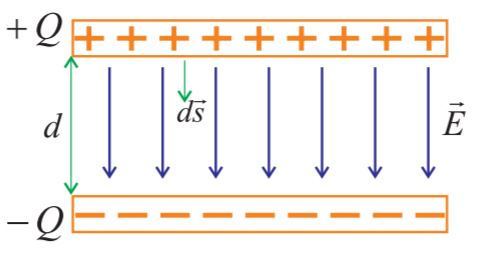
\includegraphics[scale=0.75]{notes/images/Capacitor-Electric-Field.JPG}
    \caption{Capacitor}
\end{figure}
\FloatBarrier
We will try derive capacitance in terms of the separation $d$ and the area of conducting $A$. However, we will require a new relationship that are unable to prove, as it requires knowledge of Gauss' Law which is beyond A2 Further Mathematics. 
\begin{equation}
    \label{eq:derivation-capacitance-electric-field}
    \| \vec{E} \| = \frac{Q}{\varepsilon_0 A},
\end{equation}
where $Q$ denotes charge and $A$ denotes area of conducting. Using the relationships from  \ref{eq:derivation-capacitance-electric-field} and \ref{eq:change-in-potential} and considering a path that is parallel to the electric field lines from the positive plate to the negative plate, we have
\begin{align*}
    \Delta V &= - \int_C \vec{E} \cdot \mathop{\mathrm{d}\vec{s}} \\
    &= \int_{+ve}^{-ve} \vec{E} \cdot \mathop{\mathrm{d}\vec{s}} \\ 
    &= \int_{+ve}^{-ve} \| \vec{E} \| \mathop{\mathrm{d}s} \\
    &= \frac{Q}{\varepsilon_0 A} \underbrace{\int_{+ve}^{-ve} \mathop{\mathrm{d}s}}_{\text{Length of path taken}} \\
    &= \frac{Q}{\varepsilon_0 A} d
\end{align*}
Applying the definition of capacitance to this relationship, yields a new equation for capacitance:
\begin{equation}
    C = \frac{Q}{\Delta V} = \varepsilon_0 \frac{A}{d}.
\end{equation}
When a dielectric other than a vacuum is used between the plates, the equation uses $\varepsilon$, the permittivity for the dielectric. Sometimes we use the relative permittivity $\varepsilon_r$, such that
\begin{equation}
    \varepsilon = \varepsilon_r \varepsilon_0.
\end{equation}
Therefore, the equation of capacitance may be written as
\begin{equation}
    C = \varepsilon \frac{A}{d} = \varepsilon_r \varepsilon_0 \frac{A}{d}.
\end{equation}



\subsection{Capacitors in Parallel}

\begin{theorem}{(\textbf{Capacitors in parallel})}
\textit{$n$ capacitors in parallel with potential difference $V$ across then and capacitance's $C_1, C_2, \ldots, C_n$ are isomorphic to a single capacitor with a capacitance $C_p$, where}
\begin{equation}
    C_p = \sum_{k=1}^n C_k.
\end{equation}
\begin{proof}
\textit{Consider the following circuit.}
\begin{figure}[h!]
    \centering
    \begin{circuitikz}
        \draw (0,0) to (0,6) to [battery1, v=$\varepsilon$](6,6) to [short, i=$I$](6,0) to (5,0) to (5,3) to [C = $C_1$, i=$I_1$](1,3) to (1,0) to (0,0);
        \draw (5,1) to [C = $C_2$, i=$I_2$](1,1);
        \draw (5,0) to node[below]{$\vdots$}(5,-0.5);
        \draw (5,-1.1) to (5,-1.5) to [C = $C_n$, i=$I_n$](1, -1.5) to (1, -1.1);
        \draw (1,0) to node[below]{$\vdots$}(1,-0.5);
    \end{circuitikz}
\end{figure}
\FloatBarrier
\noindent \textit{Applying Kirchhoff's first law and the definition of current to this circuit, we have}
\begin{equation*}
    I = \sum_{k=1}^n I_k \textit{ and } Q = It
\end{equation*}
\textit{combining these, it follows that}
\begin{equation*}
    Q_p = \sum_{k=1}^n Q_k
\end{equation*}
\textit{where $Q_k$ is the charge stored in the $k^{th}$ capacitor. From the definition of capacitance and Kirchhoff's second law we find that $Q_k = \varepsilon C_k$. Thus}
\begin{equation*}
    C_p = \sum_{k=1}^n C_k.
\end{equation*}
\end{proof}
\end{theorem}

\subsection{Capacitors in Series}

\begin{theorem}{(\textbf{Capacitors in Series})}
\textit{$n$ capacitors in a series arrangement with potential differences $V_1, V_2, \ldots, V_n$ across them and capacitances $C_1, C_2, \ldots, C_n$ are isomorphic to a single capacitors with a capacitance $C_s$, such that}
\begin{equation}
    \frac{1}{C_s} = \sum_{k=1}^n \frac{1}{C_k}.
\end{equation}
\begin{proof}
\textit{Consider the following circuit.}
\begin{figure}[h!]
    \centering
    \begin{circuitikz}
        \draw (0,0) to (0,3) to [battery1, v=$\varepsilon$](7,3) to [short, i=$I$](7,0) to [C = $C_1$, v=$V_1$](5,0) to [C=$C_2$, v=$V_2$](3,0);
        \draw (2,0) to node[right, xshift=0.2cm]{$\cdots$}(2,0);
        \draw (2.2,0) to (2,0) to [C=$C_n$, v=$V_n$](0,0);
    \end{circuitikz}
\end{figure}
\FloatBarrier
\noindent \textit{Applying Kirchhoff's second law, we have}
\begin{equation*}
    \varepsilon = \sum_{k=1}^n V_k
\end{equation*}
\textit{and from Kirchhoff's first law, the current $I$ entering each capacitor is equal to the current leaving each capacitor, from this it follows that each capacitor stores the same charge $Q$ coulombs. If we now apply the definition of capacitance, we find that $V_k = \frac{Q}{C_k}$, so}
\begin{align*}
    \frac{Q}{C_s} &= \sum_{k=1}^n \frac{Q}{C_k} \\
    \frac{1}{C_s} &= \sum_{k=1}^n \frac{1}{C_k}.
\end{align*}
\end{proof}
\end{theorem}

\subsection{Energy Stored in a Capacitor}

As an electron approaches the negatively charged plate of the capacitor, it experiences a repulsive electrostatic force from the electrons stored on the negative plate, so work must be done on the electron to push it onto the plate, a similar argument can be applied to pulling electrons off the positive plate. The work is provided by the cell and by the conservation of energy it follows that the energy stored in the energy stored in the capacitor is equal to the work done by the cell, which by definition is the integral of potential difference with respect to charge. 

Having rationalized this argument, we can now consider it mathematically. To charge a capacitor, we must move a small charge $\mathop{\mathrm{d}Q}$ from the $-Q$ plate  to the $+Q$ plate. This means we must do work against the potential difference, so a small amount of work $\mathop{\mathrm{d}W}$ to move a small charge $\mathop{\mathrm{d}Q}$ is given by $\mathop{\mathrm{d}W} = V \mathop{\mathrm{d}Q}$. So the total work to charge a capacitor from $0$ to $Q_1$ is given by 
\begin{equation}
    W = \int_0^{Q_1} V \mathop{\mathrm{d}Q} = \int_0^{Q_1} \frac{Q}{C} \mathop{\mathrm{d}Q} = \frac{1}{2} \frac{Q_1^2}{C} = \frac{1}{2} Q_1 V = \frac{1}{2} C V^2, 
\end{equation}
where $V$ is the potential difference across the capacitor and $C$ is the capacitance of the capacitor.

\subsection{Discharging Capacitors}
\label{subsection:discharging-capacitors}

If a capacitor is charged up by an e.m.f $\varepsilon$, then disconnected from the power supply and discharged through a resistor with resistance $R$, \textit{the charge stored will decrease exponentially}. 

We can rationalize this since as the capacitor discharges, there will be less charge stored on the plates, so the electric field strength between the plates (and thus the potential difference) will decrease. This means that the potential difference across the resistor will also decrease, and Ohm's Law predicts that then the current through the resistor will decrease too. So the rate of discharge will decrease over time. Since this rate is directly proportional to the voltage, which is in turn directly proportional to the charge stored on each plate, we have the required conditions for exponential decay. Let use analyse this a bit more mathematically, by considering the following theorem and associated proof.

\begin{theorem}{(\textbf{Discharging Capacitors})}
\textit{A discharging capacitor with capacitance $C$ and resistance $R$ in the discharge circuit can be modelled using}
\begin{equation}
    Q(t) = Q(t = 0) \exp\left(-\frac{t}{\tau}\right),
\end{equation}
\textit{where $Q(t)$ is the charge stored on each plate at time $t$ and $\tau = RC$ (the time constant).}
\begin{proof}
\textit{Let us consider a charged capacitor of $Q_0$ coulombs in the following discharge circuit}
\begin{figure}[h!]
    \centering
    \begin{circuitikz}
        \draw (0,0) to (0,2.5) to [C = $C$, v=$V$](5,2.5) to [short, i=$I$](5,0) to [R, a=$R \hspace{1mm} \ohm$](0,0);
    \end{circuitikz}
\end{figure}
\FloatBarrier
\noindent \textit{We state Ohm's Law across the resistor, $V = IR$. Now the potential difference $V$ is just $q / C$, where $q$ is the charge stored on the positive capacitor plate at some time during the discharge. Applying the definition of current to this circuit, we have}
\begin{align*}
    V &= - R \frac{\mathop{\mathrm{d}Q}}{\mathop{\mathrm{d}t}} \\ 
    \frac{1}{Q} \frac{\mathop{\mathrm{d}Q}}{\mathop{\mathrm{d}t}} &= -\frac{1}{\tau},
\end{align*}
\textit{This differential equation is solved trivially as follows}
\begin{align*}
    \int_{Q_0}^{Q_t} \frac{1}{Q} \frac{\mathop{\mathrm{d}Q}}{\mathop{\mathrm{d}t}} \mathop{\mathrm{d}t} &= - \int_0^t \frac{1}{\tau} \mathop{\mathrm{d}t} \\ 
    \int_{Q_0}^{Q_t} \frac{1}{Q} \mathop{\mathrm{d}Q} &= - \int_0^t \frac{1}{\tau} \mathop{\mathrm{d}t} \\
    \ln \left| \frac{Q_t}{Q_0} \right| &= - \frac{t}{\tau} \\
    Q_t &= Q_0 \exp \left(- \frac{t}{\tau} \right)
\end{align*}
\textit{Writing $Q_t$ explicitly as a function of time, we obtain}
\begin{equation*}
    Q(t) = Q(t = 0) \exp\left(-\frac{t}{\tau}\right).
\end{equation*}
\end{proof}
\begin{corollary}{(\textbf{Current and Voltage Equations})}
\textit{From Ohm's Law and the definition of capacitance, the decay functions for voltage and current can be derived}
\begin{equation}
    V(t) = V(t = 0) \exp\left(-\frac{t}{\tau}\right)
\end{equation}
\begin{equation}
    I(t) = I(t = 0) \exp\left(-\frac{t}{\tau}\right)
\end{equation}
\end{corollary}
\end{theorem}

Note that the we use the \textbf{time constant}. The time constant, $\tau$, is the time taken for the initial value ($Q(t = 0)$, $V(t = 0)$ or $I(t=0)$) to decrease to $\frac{1}{e} \approx 0.37$ of the initial value, hence time constant is defined as 
\begin{equation}
    \tau = RC
\end{equation}
measured in \textbf{seconds} ($s$). The time constant is the decay characteristic of these functions, similar to how half life is the decay characteristic of radioactivity. 

\subsubsection{Iterative technique for modelling exponential decay}

Instead of solving the differential equation formed in the proof above, we can apply an iterative technique to produce solutions for it. Applying the differential equation $\frac{\mathop{\mathrm{dQ}}}{\mathop{\mathrm{d}t}} = - \frac{Q}{\tau}$ to the following algorithm produces a procedure for estimating values of the decay function.

\begin{algorithm} 
    \caption{Iterative procedure for modelling exponential discharge decay function}
    \begin{algorithmic}[1]
        \Require $\tau - \text{The time constant of the discharge circuit}$
        \Require $\Delta t - \text{An incremental time period that satisfies } \Delta t \ll \tau$
        \Require $Q_0 - \text{Initial charge of the capacitor}$
        \Procedure{DecayEstimation}{$\tau, \Delta t, Q_0$}
            \If{$Q_0 \leq 0$}
                \State \textbf{return}
            \EndIf
            \State $\frac{\mathop{\mathrm{d}Q}}{\mathop{\mathrm{d}t}} \gets - \frac{Q_0}{\tau}$
            \State $\Delta Q \gets \frac{\mathop{\mathrm{d}Q}}{\mathop{\mathrm{d}t}} \Delta t$
            \State $Q_1 \gets Q_0 + \Delta Q$
            \State \textbf{output}$(Q_0, \frac{\mathop{\mathrm{d}Q}}{\mathop{\mathrm{d}t}}, \Delta Q, Q_1)$
            \State \Call{DecayEstimation}{$\tau, \Delta t, Q_1$}
        \EndProcedure 
    \end{algorithmic} 
\end{algorithm}
\FloatBarrier

\subsection{Charging Capacitors}

\begin{theorem}
\textit{A charging capacitor with capacitance $C$ and resistance $R$ in the charging circuit can be modelled using}
\begin{equation}
    Q(t) = C \varepsilon \left(1 - \exp \left( - \frac{t}{\tau} \right)\right)
\end{equation}
\textit{where $Q(t)$ is the charge stored in the capacitor at time $t$ and $\tau$ denotes the time constant.}

\begin{proof}
\textit{Imagine a DC power supply with constant e.m.f $\varepsilon$ connected in series with a capacitor $C$ and resistor $R$ (as shown below). Let $Q_0$ denote the charge of the capacitor when the potential difference across the capacitor is equal to the e.m.f (when the capacitor is fully charged), so it follows that $Q_0 = C \varepsilon$.} 
\begin{figure}[h!]
    \centering
    \begin{circuitikz}
        \draw (0,0) to [C = $C$, v=$V_C$](0,2.5) to [battery1, v=$\varepsilon$](5,2.5) to [R, l=$R \hspace{1mm} \ohm$, v=$V_R$](5,0) to [short, i=$I$](0,0);
    \end{circuitikz}
\end{figure}
\FloatBarrier
\noindent \textit{Using Kirchhoff's second law and Ohm's law, we write}
\begin{align*}
    \varepsilon - V_C &= R \frac{\mathop{\mathrm{d}Q}}{\mathop{\mathrm{d}t}} \\
    \frac{Q_0 - Q}{C} &= R\frac{\mathop{\mathrm{d}Q}}{\mathop{\mathrm{d}t}} \\
    \frac{1}{Q - Q_0} \frac{\mathop{\mathrm{d}Q}}{\mathop{\mathrm{d}t}} &= - \frac{1}{\tau}
\end{align*}
\textit{Which can be solved as shown below;}
\begin{align*}
    \int_0^{Q_t} \frac{1}{Q - Q_0} \mathop{\mathrm{d}Q} &= - \frac{1}{\tau} \int_0^t \mathop{\mathrm{d}t} \\
    \ln \left|\frac{Q_t - Q_0}{ - Q_0}\right| &= - \frac{t}{\tau} \\ 
    \frac{Q_t - Q_0}{-Q_0} &= \exp \left( - \frac{t}{\tau} \right) \\
    Q_t &= Q_0 \left( 1 - \exp \left( - \frac{t}{\tau} \right) \right)
\end{align*}
\textit{Writing $Q_t$ explicitly as a function of time, we obtain}
\begin{equation*}
    Q(t) = C \varepsilon \left( 1 - \exp \left( - \frac{t}{\tau} \right) \right)
\end{equation*}
\end{proof}
\begin{corollary}{(\textbf{Current and Voltage Equations})}
\textit{From Ohm's Law and the definition of capacitance, the exponential charging functions for voltage and current can be derived}
\begin{equation}
    V(t) = \varepsilon \left( 1 - \exp\left(-\frac{t}{\tau}\right)\right)
\end{equation}
\begin{equation}
    I(t) = \varepsilon R \left( 1 - \exp\left(-\frac{t}{\tau}\right)\right)
\end{equation}
\end{corollary}
\end{theorem}

Rationalizing these exponential charging functions can be done by considering the potential difference across and/or the current through the resistor. The current through the resistor is high initially and tends to zero as the capacitor is charged. This is because at first the capacitor is uncharged, so there is no potential difference across it and so the whole e.m.f of the supply is dissipated across the resistor. But as the capacitor gets charged, the p.d. across it opposes the e.m.f and so the p.d. across the resistor falls (since $V_0 = V_R + V_C$), as does the current (by Ohm's law). From this we can deduce that the voltage / current across the resistor can be modelled by the exponential decay equations in section \ref{subsection:discharging-capacitors}. From here the derivation is trivial. 

\section{Magnetic Force}

\subsection{Magnetic Fields}

We've seen that a particle with mass produces a gravitational field $\vec{g}$ at all points in space. In a similar manner,  a magnet is a source of a magnetic field $\vec{B}$. This can be demonstrated by moving a compass near a magnet as shown in figure \ref{fig:bar-magnet}.

\begin{figure}[h!]
    \centering
    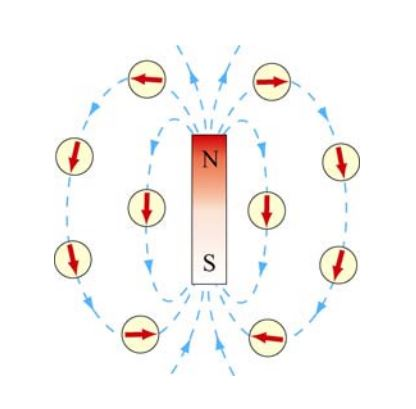
\includegraphics[scale=0.6]{notes/images/Magnetism-1.JPG}
    \caption{Magnetic field produced by a bar magnet}
    \label{fig:bar-magnet}
\end{figure}
\FloatBarrier

Notice that a magnet consists of two poles, which are designated as the north and south poles. The magnetic field lines leave from the north pole and enter the south pole. Meaning that opposite poles are attracted to each other, while the like poles will repel each other. 

\begin{figure}[h!]
    \centering
    \includegraphics{notes/images/Magnetism-2.JPG}
    \caption{Magnets attracting and repelling}
\end{figure}
\FloatBarrier

Unlike a gravitational field, a magnetic field is \textbf{dipole} in nature. Meaning that magnetic ``monopoles'' do not exist in isolation. So the definition of the magnetic field $\vec{B}$ cannot exist in the following form
\begin{equation}
    \vec{B} = \frac{\vec{F}}{q_{mag}},
\end{equation}
where $q_{mag}$ is the ``magnetic charge'' of a positive magnetic test charge and $\vec{F}$ is the force acting on it. As we cannot break a magnet in half to get a north pole and a south pole. So we must look for other interactions with a magnetic force to define the magnetic field. 

It turns out that an electrically charged object (like an electron) can be accelerated by a magnetic force, and through that interaction we can define the magnetic field. To define the field at a point, consider a particle of charge $q$ and moving at a velocity $\vec{v}$. Experimentally we have the following observations:
\begin{enumerate}
    \item The magnitude of the magnetic force $\vec{F}$ exerted on the charged particle is proportional to both the magnitude of the velocity and charge.
    \item The magnitude and direction of $\vec{F}$ depends on $\vec{v}$ and $\vec{B}$.
    \item The magnitude of $\vec{F}$ is zero when $\vec{v}$ is parallel to $\vec{B}$. However, when $\vec{v}$ makes an angle $\theta$ with $\vec{B}$, the direction of $\vec{B}$ is perpendicular to the plane formed by $\vec{v}$ and $\vec{B}$ and the magnitude of $\vec{F}$ is proportional to $\sin \theta$.
    \item When the sign of the charge of the particle is switched (i.e from positive to negative), the direction of the force also reverses. 
\end{enumerate}
The above can be summarized with the following equation
\begin{equation}
    \vec{F} = q\vec{v} \times \vec{B}
\end{equation}
and the magnitude of $\vec{F}$ is given by
\begin{equation}
    \| \vec{F} \| = |q|\| \vec{v}\|\|\vec{B}\| \sin \theta
\end{equation}
The magnitude of the magnetic field $\vec{B}$, denoted $\| \vec{B} \|$, is referred to the \textbf{magnetic flux density} of the field. The $SI$ unit for magnetic flux density is the \textbf{tesla} ($T$):
\begin{equation}
    \left[T\right] = \left[\frac{N}{C \cdot ms^{-1}}\right] = \left[\frac{N}{A \cdot m}\right] = \left[kgA^{-1}s^{-1}\right]
\end{equation}

\subsection{Magnetic Fields and Work}

Let us now consider the work done on a charged particle by the magnetic force moving from position $1$ to $2$, that is
\begin{equation}
    W = \int_C \vec{F} \cdot \mathop{\mathrm{d}\vec{s}}. 
\end{equation}

Using equation ?? and re-writing $\mathop{\mathrm{d}\vec{s}}$ as $\vec{v}\mathop{\mathrm{d}t}$, we find that
\begin{equation}
    W = \int_C (q\vec{v} \times \vec{B}) \cdot \vec{v} \mathop{\mathrm{d}t}.
\end{equation}

We know that the magnetic force $\vec{F}$ is always perpendicular to velocity and the magnetic field, so from the definition of the scalar product it follows that $\vec{F} \cdot \vec{v}$ is zero. So $W = 0$ and no work is done by the magnetic field! (\textit{What a shock! How is this possible, motion with no work done!}). This implies that there is no change in energy of a charged particle being accelerated by a magnetic force, only a change in direction. 

\subsection{Magnetic Force and Circular Motion}

Recall that the magnetic force is perpendicular to the direction of motion. This implies that the trajectory of a charged particle in a uniform magnetic field is a circle in the plane perpendicular to the direction of the motion. 

Consider a charged particle with velocity $\vec{v}$ (taken to be towards the right) entering a region of uniform magnetic field point into the plane of the page. The particle will be deflected by a force that is perpendicular to the field and the initial velocity. In the example below, this will be in the upwards direction. But when recalculating the force at another point along the trajectory, we will find that the particle is continually deflect with an equal magnitude force, and the net effect is a circular orbit. Since the magnetic field does not work, the radius of the circle $r$ will be constant.

\begin{figure}[h!]
    \centering
    \includegraphics[scale=0.6]{notes/images/Magnetism-CM.JPG}
    \caption{Circular motion in a uniform magnetic field}
\end{figure}
\FloatBarrier

As our force acts radially, we can apply equations ?? and ?? and add a radial unit vector $\hat{r}$ to obtain
\begin{equation}
    \vec{F} = \frac{m \| \vec{v} \|^2}{r} \hat{r} = |q| \| \vec{v} \| \|\vec{B}\| \hat{r},
\end{equation}
solving for our radius $r$ of circular motion gives
\begin{equation}
    r = \frac{m \| \vec{v} \|}{|q| \| \vec{B} \|}.
\end{equation}
In other words, since momentum is defined as $\vec{p} = m \vec{v}$, we have
\begin{equation}
    r = \frac{\| \vec{p} \|}{|q| \| \vec{B} \|}.
\end{equation}
The time period for a single revolution, referred to as the \textbf{Cyclotron period}, is
\begin{equation}
    T = \frac{2\pi r}{\| \vec{v} \|} = \frac{2\pi m}{|q| \| \vec{B} \|}.
\end{equation}
    
\subsection{Lorentz Force}

In the presence of both a electric field $\vec{E}$ and a magnetic field $\vec{B}$, the resultant force, referred to as the \textbf{Lorentz force}, on the charged particle is
\begin{equation}
    \vec{F} = q(\vec{E} + \vec{v} \times \vec{B})
\end{equation}

By combining the two fields, particles can have their velocity selected. This principle was first used by J.J. Thomson to measure the charge-to-mas ratio of the electron. Figure \ref{fig:lorentz-force} illustrates Thomson's apparatus.

\begin{figure}[h!]
    \centering
    \includegraphics[scale=0.75]{notes/images/Lorentz-Force.JPG}
    \caption{Thomson's apparatus}
    \label{fig:lorentz-force}
\end{figure}
\FloatBarrier

The electrons with charge $q = -e$ and mass $m_e$ are emitted from the electron gun with velocity $\vec{v}_0$ . When the electrons pass through a region where there exists a downward uniform electric field, the electrons, being negatively charged will be deflected upwards. So only considering the electric field $\vec{E}$ we have vertical acceleration $\vec{a}_y$
\begin{equation}
    \vec{a}_y = \frac{e \| \vec{E}\|}{m_e} 
\end{equation}
    
The electric field $\vec{E}$ occupies a region of length $\ell$. We assume the electrons emitted from the electron gun only have a horizontal component for velocity. So the time to cross the region is given by
\begin{equation}
    t \approx \frac{\ell}{\| \vec{v}_0 \|}.
\end{equation}
By definition, the vertical component of velocity $\vec{v}_y$ upon exit of the region is then
\begin{equation}
    \vec{v}_y = \vec{a}_y t = \frac{e \|\vec{E}\| \ell}{m_e \| \vec{v}_0 \|}
\end{equation}
So the tangent of the exit angle is
\begin{equation}
    \tan \theta = \frac{e \| \vec{E} \| \ell}{m_e \| \vec{v}_0 \|^2}
\end{equation}
The angle $\theta$ and the length of the electric plates can be measured experimentally. The electric field strength can be determined from the potential difference applied across the plates divided by the separation, 
\begin{equation}
    \| \vec{E} \| = \frac{V}{d}
\end{equation}

We can determine the initial velocity using an energy consideration in the electron gun. Alternatively, we could configure the magnetic field such that the beam of electrons is no longer deflected. That is the Lorentz force acting on the electron is zero, $\vec{F} = q(\vec{E} + \vec{v} \times \vec{B}) = \vec{0}$, so we have
\begin{align}
    \vec{E} &= - \vec{v} \times \vec{B} \\
    &= \| \vec{v}_0 \| \| \vec{B} \|
\end{align}
So the initial velocity is
\begin{equation}
    \| \vec{v}_0 \| = \frac{\| \vec{E} \|}{\| \vec{B} \|}
\end{equation}
Armed with this, we can determine the charge-to-mass ratio of an electron:
\begin{equation}
    \tan \theta = \frac{e \| \vec{E} \| \ell}{m_e} \frac{\|\vec{B}\|^2}{\| \vec{E} \|^2} 
\end{equation}
Rearranging this for $e / m_e$ gives
\begin{equation}
    \frac{e}{m_e} = \frac{\| \vec{E} \| \tan \theta}{\| \vec{B} \|^2 \ell}
\end{equation}
\subsection{The Hall Effect}    

Consider charges travelling in a conducting wire with a external magnetic field acting on the charges. The charges will be \textit{pushed to one side of the wire by the magnetic force}. This separation of charge in the wire is called the \textbf{Hall Effect}. 

\begin{figure}[h!]
    \centering
    \includegraphics[scale=0.4]{notes/images/Hall-Effect.JPG}
    \caption{The Hall Effect}
\end{figure}
\FloatBarrier

The separation will stop when the magnetic force $\vec{F}_B$ experienced by the charge carriers is balanced by the force $\vec{F}_H$ caused by the electric field due to the separation of charged. We define the \textbf{Hall voltage} $\Delta V_H$ as the potential difference across the width of the wire. Therefore the electrical field strength of the electric field produced by the separated charges is \begin{equation}
    \| \vec{E} \| = \frac{\Delta V_H}{W},
\end{equation}
where $W$ is the width of the wire (or conducting strip). In equilibrium our Lorentz force is zero, hence $q(\vec{E} + \vec{v} \times \vec{B}) = \vec{0}$ meaning we can apply our special case we discussed in the previous section (see equation ??), giving us
\begin{equation}
    \frac{\Delta V_H}{W} = \| \vec{v} \| \| \vec{B}\|.
\end{equation}
Recall that current is given by $I = ne\| \vec{v} \|A$, where $n$ is the number density of the conductor. So we have
\begin{equation}
    \frac{\Delta V_H}{W} = \frac{I\| \vec{B}\|}{neA}.
\end{equation}
We note that $A = Wh$, where $h$ is the height of the conductor, giving
\begin{equation}
    \Delta V_H = \frac{I\| \vec{B}\|}{neh}.
\end{equation}

This equation has two main applications, determining the charge density of the conductor using the following equation
\begin{equation}
    n = \frac{I\| \vec{B}\|}{qh\Delta V_H}.
\end{equation}
Alternatively, we can then measure the magnetic flux density of the magnetic field provided we know the Hall voltage, current and number density of the conductor.
\begin{equation}
    \| \vec{B} \| = \frac{neh}{I} \Delta V_H.
\end{equation}

\subsection{Magnetic Force on Currents}

We've just seen that a charged particle moving through a magnetic field experiences a magnetic force $\vec{F}$. Since electric current consists of a charged particles in motion, when placed in a magnetic field, a wire will also experience a force. 

Consider a straight wire suspended in a region between two magnetic poles. The magnetic field points out of the page and is represented with dots (this is known as the ``arrow'' convention, where the dot represents an arrow head heading towards us and the arrow cross-hairs heading away from us are represented by crosses). Experimentally, we see when a downwards current passes through, the wire is deflected towards the left. However, when the current is upwards, the deflections is rightwards. (See figure \ref{fig:magnetic-field-wire-1}).

\begin{figure}[h!]
    \centering
    \includegraphics{notes/images/Magnetic-Field-Wire-1.JPG}
    \caption{Deflection of current-carrying wire by magnetic force}
    \label{fig:magnetic-field-wire-1}
\end{figure}
\FloatBarrier

To calculate the force exerted on the wire, consider a segment of the wire with length $\ell$ and a cross sectional area of $A$, as illustrated below. The magnetic field points into the page and is represented by crosses. 

\begin{figure}[h!]
    \centering
    \includegraphics{notes/images/Magnetic-Field-Wire-2.JPG}
    \caption{Magnetic force on a conducting wire}
    \label{fig:magnetic-field-wire-2}
\end{figure}
\FloatBarrier

The charges moves with a mean drift velocity $\vec{v}_{drift}$. Since the total amount of charge in this segment is $Q_{total} = qnA\ell$, where $n$ is the number density of the conductor. So the total magnetic force acting on this segment is
\begin{equation}
    \vec{F} = Q_{total} (\vec{v}_{drift} \times \vec{B}) = qnA\ell (\vec{v}_{drift} \times \vec{B}) = I (\vec{\ell} \times \vec{B}).
\end{equation}
where $I = nqv_{drift}A$, and $\vec{\ell} = \ell \hat{\ell}$ is a \textit{length vector} with a magnitude $\ell$ and directed along the direction of the electric current or wire. So the magnitude of the magnetic force is given by
\begin{equation}
    \| \vec{F} \| = \| \vec{B} \| I \ell \sin \theta,
\end{equation}
where $\theta$ is the angle between the direction of current and the magnetic field lines. 

For a wire of arbitrary shape, the magnetic force can be obtained by summing over the forces acting on the small segments that make up the wire. Let the differential segment of the wire be denoted as $\mathop{\mathrm{d}\vec{s}}$. 

\begin{figure}[h!]
    \centering
    \includegraphics{notes/images/Magnetic-Field-Wire-3.JPG}
    \caption{Current-carrying wire in a magnetic field}
    \label{fig:magnetic-field-wire-3}
\end{figure}
\FloatBarrier

The magnetic force acting on the segment is 
\begin{equation}
    \mathop{\mathrm{d}\vec{F}} = I(\mathop{\mathrm{d}\vec{s} \times \vec{B}}).
\end{equation}
Thus the total force is
\begin{equation}
    \vec{F} = I \int_C \mathop{\mathrm{d}\vec{s}} \times \vec{B}.
\end{equation}
However as a magnetic field is a conservative field, the integral only depends on the initial and finial positions of the charged particle, thus we can rewrite the equation above as
\begin{equation}
    \label{eq:magnetic-force-on-wire-integral}
    \vec{F} = I \int_a^b \mathop{\mathrm{d}\vec{s}} \times \vec{B},
\end{equation}
where $a$ and $b$ represent the endpoints of the wire.

So for example, consider a curved wire carrying a current $I$ in a uniform magnetic field $\vec{B}$ as shown in figure \ref{fig:magnetic-field-wire-4}.

\begin{figure}[h!]
    \centering
    \includegraphics{notes/images/Magnetic-Field-Wire-4.JPG}
    \caption{A curved wire with a current $I$}
    \label{fig:magnetic-field-wire-4}
\end{figure}
\FloatBarrier

Using equation \ref{eq:magnetic-force-on-wire-integral}, the magnetic force on the wire is given by
\begin{equation}
    \vec{F} = I \left(\int_a^b \mathop{\mathrm{d}\vec{s}}\right) \times \vec{B} = I(\vec{\ell} \times \vec{B})
\end{equation}
where $\vec{\ell}$ is the length vector directed from $a$ to $b$. However, if the wire forms a closed loop of arbitrary shape, then the force on the loop becomes
\begin{equation}
    \vec{F} = I \int_a^a \mathop{\mathrm{d}\vec{s}} \times \vec{B}.
\end{equation}

\begin{figure}[h!]
    \centering
    \includegraphics{notes/images/Magnetic-Field-Wire-5.JPG}
\end{figure}
\FloatBarrier

Since the set of differential length elements $\mathop{\mathrm{d}\vec{s}}$ forms a closed polygon, and their vector sum is zero. The net magnetic force on a closed loop is $\vec{F} = \vec{0}$.

\begin{experiment}
Determining magnetic flux density TODO
\end{experiment}

Alternatively, we could consider what happens when we place a rectangular loop carrying a current $I$ in the $x - y$ plane and switch on a uniform magnetic field that runes parallel to the plane of the current, that is $\vec{B} = \| \vec{B} \| \hat{i}$, as shown in the figure below.

\begin{figure}[h!]
    \centering
    \includegraphics{notes/images/Magnetic-Feild-Current-Loop.JPG}
    \caption{(a) A rectangular current loop placed in a uniform magnetic field. (b) The magnetic forces acting on sides $2$ and $4$}
\end{figure}
\FloatBarrier

We see the magnetic forces acting on sides $1$ and $3$ vanish because their length vectors $\ell_1 = -b \hat{i}$ and $\ell_3 = b \hat{i}$ are parallel and anti-parallel to $\vec{B}$ and their cross products vanish. On the other hand, the magnetic forces acting on segments $2$ and $4$ are non-vanishing
\begin{align}
    \vec{F}_2 &= I(-a\vec{j} \times \| \vec{B} \|\hat{i}) = Ia\|\vec{B}\| \hat{k} \\
    \vec{F}_4 &= I(a\vec{j} \times \| \vec{B} \|\hat{i}) = - Ia\|\vec{B}\| \hat{k} 
\end{align}
with $\vec{F}_2$ pointing out of the page and $\vec{F}_4$ into the page. Thus, the resultant force on the rectangular loop is
\begin{equation}
    \vec{F} = \vec{F}_1 + \vec{F}_2 + \vec{F}_3 + \vec{F}_4 = \vec{0},
\end{equation}
which is a special case of equation ??, as discussed earlier. Even though the resultant force is zero, the forces $\vec{F}_2$ and $\vec{F}_4$ will produce a torque which causes the loop to rotate about the $y$-axis. 
The resultant torque (from equation ??) with respect to the center of the loop is
\begin{align}
    \vec{\tau} &= \vec{\tau}_2 + \vec{\tau}_4 \\
    &= \left(-\frac{b}{2}\hat{i} \times \vec{F}_2\right) + \left(\frac{b}{2}\hat{i} \times \vec{F}_4\right) \\
    &= Iab\|\vec{B}\|\hat{j} = IA\|\vec{B}\|\hat{j},
\end{align}
where $A=ab$ represents the area of the loop and the positive sign indicates the the rotation is clockwise about the $y$-axis. In is convenient to introduce the vector area $\vec{A} = A\hat{n}$, where $\hat{n}$ is the surface vector of the loop. The direction of $\hat{n}$ is set by the conventional right-hand rule. In this special case (i.e. when $\theta = \pi/2$) we have $\hat{n} = \hat{k}$. So the above expression for torque can be rewritten as
\begin{equation}
    \vec{\tau} = I \vec{A} \times \vec{B}. 
\end{equation}

Consider now the more general situation where the loop (or the vector area $\vec{A}$) makes an angle $\theta$ with respect to the magnetic field $\vec{B}$. 

\begin{figure}[h!]
    \centering
    \includegraphics{notes/images/Magnetic-Fields-Current-Loop-2.JPG}
    \caption{Rotation of a rectangular current loop.}
    \label{fig:magnetic-field-current-loop-2}
\end{figure}
\FloatBarrier

From Figure \ref{fig:magnetic-field-current-loop-2}, we can see that
\begin{align}
    \vec{r}_2 &= \frac{b}{2} \left(-\cos\left(\frac{\pi}{2} - \theta\right) \hat{i} + \sin\left(\frac{\pi}{2} - \theta\right)\hat{k}\right) \\
    &= \frac{b}{2}\left(\cos(\theta) \hat{k} - \sin (\theta) \hat{i}\right) \\
    &= - \vec{r}_4
\end{align}
and the resultant torque $\vec{\tau}$ becomes
\begin{align}
    \vec{\tau} &= \vec{r}_2 \times \vec{F}_2 + \vec{r}_4 \times \vec{F}_4 \\
    &= 2 \vec{r}_2 \times \vec{F}_2 \\
    &= 2 \frac{b}{2}\left(\cos(\theta) \hat{k} - \sin (\theta) \hat{i}\right) \times \left(Ia\| \vec{B} \| \hat{k}\right) \\
    &= Iab\| \vec{B} \| \sin \theta \hat{j} \\
    &= I \vec{A} \times \vec{B}
\end{align}
For a loop consisting of $N$ turns, the resultant torque is
\begin{equation}
    \vec{\tau} = NI \vec{A} \times \vec{B}.
\end{equation}
We define the quantity $NI\vec{A}$ as the magnetic dipole moment $\vec{\mu}$:
\begin{equation}
    \vec{\mu} = NI\vec{A}
\end{equation}

\begin{figure}[h!]
    \centering
    \includegraphics{notes/images/Magnetic-Fields-Current-Loop-3.JPG}
    \caption{Right-hand rule for determining the direction of $\vec{\mu}$.}
    \label{fig:magnetic-field-current-loop-3}
\end{figure}
\FloatBarrier

The direction of $\vec{\mu}$ is parallel to the vector area $\vec{A}$ (perpendicular to the plane of the loop) and is determined by a right-hand rule (figure \ref{fig:magnetic-field-current-loop-3}). Using the expression for $\vec{\mu}$, the torque exerted on the loop can be rewritten as
\begin{equation}
    \vec{\tau} = \vec{\mu} \times \vec{B}
\end{equation}

The work done by an external force to rotate the magnetic dipole from an angle $\theta_1$ to $\theta_2$ is given by (see equation ??)
\begin{align}
    W_{external} &= \int_{\theta_1}^{\theta_2} \| \vec{ \tau} \| \mathop{\mathrm{d}\theta} \\
    &= \int_{\theta_1}^{\theta_2} \| \vec{\mu} \| \vec{B} \| \sin \theta \mathop{\mathrm{d}\theta} \\
    &= \|\vec{\mu}\|\|\vec{B}\|(\cos \theta_1 - \cos \theta_2)
\end{align}
We say that $W_{external} = -W = \Delta E_p = E_{p,2} - E_{p,1} $, where $W$ is the work done by the magnetic field. Choosing $E_{p,1} = 0$ at $\theta_1 = \pi/2$, the dipole in the presence of an external field then has a potential energy of
\begin{equation}
    E_p = - \| \vec{\mu} \| \| \vec{B} \| \cos \theta = - \vec{\mu} \cdot \vec{B}.
\end{equation}

\subsubsection*{A Note on Fleming's Left-Hand Rule}

If we consider $\vec{B}$ and $\vec{v}$ being perpendicular, that is $\theta = \pi/2$ then we see that the magnetic force direction on a current-carrying wire in a uniform magnetic field is given by a left-hand rule, known as \textbf{Fleming's left-hand rule}. We use our left hands as shown in figure \ref{fig:fleming-left-hand}.

\begin{figure}[h!]
    \centering
    \includegraphics[scale=0.6]{notes/images/Fleming-Left-Hand.JPG}
    \caption{Fleming's left-hand rule}
    \label{fig:fleming-left-hand}
\end{figure}
\FloatBarrier

\noindent The direction of our:
\begin{itemize}
    \item \textbf{Thumb}: is the direction of our magnetic force (or motion, provided the resultant force is parallel to the magnetic force).
    \item \textbf{First finger}: is the direction of the magnetic field lines (north to south). 
    \item \textbf{Second finger}: is the direction of the \textit{convention current} through the wire. 
\end{itemize}

\section{Magnetic Fields}

\subsection{Magnetic Fields}

A moving charge can either experience a magnetic force in a magnetic field $\vec{B}$, or it can generate a magnetic field. We say the magnetic field $\vec{B}$ at point $P$ generated by a charge $q$ in space moving with a velocity $\vec{v}$ is given by
\begin{equation}
    \vec{B} = \frac{\mu_0}{4\pi} \frac{q \vec{v} \times \hat{r}}{\| \vec{r} \|^2},
\end{equation}
where $\mu_0$ is the so called \textbf{permeability of free space}. a magnetic constant, $\mu_0 = 4\pi \times 10^{-7}$ $TmA^{-1}$. This is the formal definition of a magnetic field. 

\begin{figure}[h!]
    \centering
    \includegraphics[scale=0.8]{notes/images/Magnetic-Field-Definition-1.JPG}
\end{figure}
\FloatBarrier

From equation ?? we can make some observations, the most obvious being that when $\theta = \pi/2$ the magnetic field experienced at point $P$ is at a maximum and when $\theta = 0, 2\pi$ the magnetic field experienced at point $P$ is at a minimum. 

\begin{figure}[h!]
    \centering
    \includegraphics[scale=0.8]{notes/images/Magnetic-Field-Definition-2.JPG}
\end{figure}
\FloatBarrier

So for example, considering the figure above. The magnetic field $\vec{B}$ at $P_0$ is zero, the same can be said for the magnetic field at $P_1$. Whereas the magnetic field at $P_2$ isn't zero, however it is less than the magnetic field at $P_3$. 

Despite our definition of a magnetic field, experimentally we see that a single moving charge will \textit{not} generate a steady magnetic field. As discussed in section ??, stationary charges will generate a steady electric field $\vec{E}$, similarly, steady currents will generate a steady magnetic field $\vec{B}$. 

So a magnetic field at the point $P$ can be obtained by \textit{integrating} the contribution from individual current segments, this is known as the \textbf{principle of magnetic superposition}. By considering a small charge $\mathop{\mathrm{d}q}$ we have 
\begin{equation}
    \mathop{\mathrm{d}\vec{B}} = \frac{\mu_0}{4\pi} \frac{\mathop{\mathrm{d}q} \vec{v} \times \hat{r}}{\| \vec{r} \|^2}
\end{equation}

\begin{figure}[h!]
    \centering
    \includegraphics[scale=0.4]{notes/images/Magnetic-Superposition-1.JPG}
\end{figure}
\FloatBarrier

Notice that $\mathop{\mathrm{d}q} \vec{v} = \mathop{\mathrm{d}q} \frac{\mathop{\mathrm{d}\vec{s}}}{\mathop{\mathrm{d}t}} = I \mathop{\mathrm{d}\vec{s}}$, so 
\begin{equation}
    \mathop{\mathrm{d}\vec{B}} = \frac{\mu_0}{4\pi} \frac{I \mathop{\mathrm{d}\vec{s}} \times \hat{r}}{\| \vec{r} \|^2}.
\end{equation}
This is known as the \textbf{Biot-Savart Law} and will allow us to find the magnetic field generated by a circuit. For the current around a whole circuit
\begin{equation}
    \vec{B} = \int_C \mathop{\mathrm{d}\vec{B}} = \int_C \frac{\mu_0}{4\pi} \frac{I \mathop{\mathrm{d}\vec{s}} \times \hat{r}}{\| \vec{r} \|^2},
\end{equation}
where the curve $C$ is the topological representation of the circuit. 



We've just seen that a current in a circuit will generate a magnetic field $\vec{B}$. Consider a straight wire as shown in figure ??. We will consider an individual current segment $I \mathop{\mathrm{d}\vec{s}} = I \mathop{\mathrm{d}y} \hat{s}$ in a wire of length $\ell$ to find the magnetic field $\vec{B}$ at the point $P$. 

\begin{figure}[h!]
    \centering
    \includegraphics[scale=0.5]{notes/images/Magnetic-Field-Wire-P-1.JPG}
\end{figure}
\FloatBarrier

Abstracting the above figure geometrically gives

\begin{figure}[h!]
    \centering
    \includegraphics[scale=0.35]{notes/images/Magnetic-Field-Wire-P-2.JPG}
\end{figure}
\FloatBarrier

So the magnitude of $\mathop{\mathrm{d}\vec{s}} \times \hat{r}$ is given by
\begin{align}
    \| \mathop{\mathrm{d}\vec{s}} \times \hat{r} \| &= \mathop{\mathrm{d}y} \sin \theta \\
    &= \mathop{\mathrm{d}y} \sin (\pi - \theta) \\
    &= \mathop{\mathrm{d}y} \frac{x}{\| \vec{r} \|} \\
    &= \frac{x \mathop{\mathrm{d}y}}{\sqrt{x^2 + y^2}}
\end{align}
Applying the Biot-Savart Law produces the following relationship
\begin{align}
    \| \mathop{\mathrm{d}\vec{B}} \| &= \frac{\mu_0}{4\pi} \frac{Ix \mathop{\mathrm{d}y}}{(x^2 + y^2)^{3/2}}
\end{align}
Integrating over the current in the wire gives
\begin{equation}
    \| \vec{B} \| = \int_{-\ell/2}^{\ell/2} \frac{\mu_0}{4\pi} \frac{Ix \mathop{\mathrm{d}y}}{(x^2 + y^2)^{3/2}} = \frac{\mu_0 I x}{4 \pi} \int_{-\ell/2}^{\ell/2} \frac{\mathop{\mathrm{d}y}}{(x^2 + y^2)^{3/2}}
\end{equation}
This integral can be solved trivially via a trigonometric substitution of $y = x \tan u$, thus
\begin{equation}
    \| \vec{B} \| = \frac{\mu_0I}{4\pi x} \frac{\ell}{\sqrt{x^2 + \frac{\ell^2}{4}}}
\end{equation}
The direction of the magnetic field $\vec{B}$ can be determined via a right-hand corkscrew rule shown in the figure below. 

However, if the straight wire forms a circular current loop, then the magnetic field generated is different. In a similar fashion, let us consider a current segment $I\mathop{\mathrm{d}\vec{s}}$ on the current loop and the magnetic field generated at some point $P$, as shown in figure \ref{fig:magnetic-field-current-loop-p-1}.

\begin{figure}[h!]
    \centering
    \includegraphics[scale=0.4]{notes/images/Magnetic-Feild-Current-Loop-P-1.JPG}
    \caption{(a) Geometric interpretation of two current segments in a current loop. (b) Current segment consideration in a current loop.}
    \label{fig:magnetic-field-current-loop-p-1}
\end{figure}
\FloatBarrier

Notice that for every current element $I \mathop{\mathrm{d}\vec{s}_1}$, generating a magnetic field $\mathop{\mathrm{d}\vec{B}_1}$ at point $P$, there is an opposite current element $I\mathop{\mathrm{d}\vec{s}_2}$, generating a magnetic field $\mathop{\mathrm{d}\vec{B}_2}$ such that
\begin{equation}
    \mathop{\mathrm{d}\vec{B}_1} \sin \alpha = - \mathop{\mathrm{d}\vec{B}_2} \sin \alpha
\end{equation}
Hence we only need to consider the vertical component of $\vec{B}$ needs to be considered at $P$. We also note that $\mathop{\mathrm{d}\vec{s}}$ is perpendicular to $\hat{r}$, so the magnitude of our vector product is simply $\mathop{\mathrm{d}s}$. So applying the Biot-Savart Law, gives
\begin{equation}
    \| \mathop{\mathrm{d}\vec{B}} \| = \frac{\mu_0}{4 \pi} \frac{I\mathop{\mathrm{d}s}}{\| \vec{r} \|^2}
\end{equation}
Integrating around the circuit yields our magnetic field $\vec{B}$ at $P$
\begin{align}
    \| \vec{B} \| &= \int_C \| \mathop{\mathrm{d}\vec{B}} \| \cos \alpha
\end{align}
We're multiplying the integral by $\cos \alpha$ as we're only interested in the vertical component of $\vec{B}$. Given we're considering a circular current loop, we can integrate from $0$ to $2\pi$. So 
\begin{align}
    \| \vec{B} \| &= \int_0^{2\pi} \frac{\mu_0}{4\pi} \frac{I \mathop{\mathrm{d}s}}{\| \vec{r} \|^2} \frac{R}{\| \vec{r} \|} \\
    &= \frac{IR\mu_0}{4\pi \| \vec{r} \|^3} \int_0^{2\pi} \mathop{\mathrm{d}s}
\end{align}
The integral $\int_0^{2\pi} \mathop{\mathrm{d}s}$ is simply the circumference of the circle, hence
\begin{align}
    \| \vec{B} \| &= \frac{IR^2 \mu_0}{2 \| \vec{r} \|^3} \\
    &= \frac{IR^2\mu_0}{2(R^2 + y^2)^{3/2}}
\end{align}
Similarly, the direction of the magnetic field $\vec{B}$ can be determined from the right hand corkscrew rule, where our thumb represents the direction of $\vec{B}$ and our fingers represent the direction of conventional current in the loop. Our interest in the circular current loop is because we can formally define a circular current loop as a \textbf{magnetic dipole}. We will also use this result to consider the magnetic field produce by a solenoid. 

A solenoid is commonly used to produce a \textit{strong} and \textit{uniform} magnetic field insides it's coils. Consider a solenoid of length $\ell$ consisting of $N$ turns of wire. We define $n$ as the number of turns per a unit of length, that is
\begin{equation}
    n = \frac{N}{\ell}.
\end{equation}

We note that a solenoid can be approximated by a series of tightly-packed coils of wire. This will allow us to utilise the expression for a magnetic field produced by a current loop we derived earlier.

\begin{figure}[h!]
    \centering
    \includegraphics[scale=0.4]{notes/images/Solenoid-1.JPG}
\end{figure}

Now consider the magnetic field $\vec{B}$ at a distance $x'$ from the center of the solenoid. For a current segment we will need to consider a coil segment of length $\mathop{\mathrm{d}x}$, as shown below.

\begin{figure}[h!]
    \centering
    \includegraphics[scale=0.4]{notes/images/Solenoid-2.JPG}
    \caption{(a) Current segment consideration in a solenoid. (b) Geometric interpretation of current segment in a solenoid.}
\end{figure}
\FloatBarrier

Hence the number of current turns in said segment is $n \mathop{\mathrm{d}x}$. Multiplying this by the current gives us the net current $I_c$ in the coil segment, that is

\begin{equation}
    I_c = In\mathop{\mathrm{d}x}.
\end{equation}

Using the result from one coil / current loop in equation ??, we obtain the magnetic field $\vec{B}$ produced by the coil segment of length $\mathop{\mathrm{d}x}$ at a distance of $x$ from the center:
\begin{equation}
    \| \mathop{\mathrm{d}\vec{B}} \| = \frac{R^2 (In\mathop{\mathrm{d}x}) \mu_0}{2 \| \vec{r} \|^3}
\end{equation}

As clearly shown in the figure above, $\| \vec{r} \| = \sqrt{R^2 + (x - x')^2}$. So integrating over the entire solenoid gives
\begin{align}
    \| \vec{B} \| &= \int_{-\ell/2}^{\ell/2} \| \mathop{\mathrm{d}\vec{B}} \| \\
    &= \frac{IR^2n\mu_0}{2} \int_{-\ell/2}^{\ell/2} \frac{\mathop{\mathrm{d}x}}{\left(R^2 + (x - x')^2\right)^{3/2}}
\end{align}
The integral can be solved trivially via a substitution of $u = x - x'$ followed by a trigonometric substitution of $u = R\tan v$, thus
\begin{equation}
    \| \vec{B} \| = \frac{I n \mu_0}{2} \left[\frac{\frac{\ell}{2} + x'}{\sqrt{\left(\frac{\ell}{2} + x'\right)^2 + R^2}} + \frac{\frac{\ell}{2} - x'}{\sqrt{\left(\frac{\ell}{2} - x'\right)^2 + R^2}}\right]
\end{equation}
along the positive $x$ direction. The direction of the magnetic field can be determined using a right-hand corkscrew rule, as shown in the figure below. 

\begin{figure}[h!]
    \centering
    \includegraphics[scale=0.3]{notes/images/Solenoid-RHR.JPG}
    \caption{Right-hand corkscrew rule for a solenoid.}
\end{figure}
\FloatBarrier

\subsection{Ampere's Law}

In our study of magnetism we often try to calculate the magnetic field $\vec{B}$ for highly symmetrical objects, such as a wire, circular current loop or solenoid. So far we've been considering each object independently and applying the Biot-Savart Law. However, we can apply \textbf{Ampere's Law} instead which states the line integral around a closed curve $C$, referred to as an \textbf{Amperian curve}, of a magnetic field $\vec{B}$ with respect to displacement $\vec{s}$ is $I_c \mu_0$, that is
\begin{equation}
    \int_C \vec{B} \cdot \mathop{\mathrm{d}\vec{s}} = I_c \mu_0,
\end{equation}
where $I_c$ is the net current that penetrates the area bounded by the curve $C$. 
\subsubsection*{A note on convention} 
We commonly use the right-hand corkscrew rule to determine the \textit{sign} of the current. So for example, consider the currents $I_1, I_2, I_3$ and $I_4$ and the Amperian curve $C$ as shown in figure \ref{fig:ampere-law-1}. We have
\begin{align}
    \int_C \vec{B} \cdot \mathop{\mathrm{d}\vec{s}} &= \mu_0 (I_1 - I_3 + I_4 - I_4) \\
    &= \mu_0 (I_1 - I_3)
\end{align}

\begin{figure}[h!]
    \centering
    \includegraphics[scale=0.4]{notes/images/Ampere-Law-1.JPG}
    \caption{Ampere's Law Example}
    \label{fig:ampere-law-1}
\end{figure}
\FloatBarrier

We will now consider our previous results for the magnetic field of a wire and solenoid, however, we will consider them with respect to Ampere's law instead of the Biot-Savart law. 

For a straight wire, construct an Amperian curve $C$ of radius $x$ as illustrated below.

\begin{figure}[h!]
    \centering
    \includegraphics[scale=0.3]{notes/images/Ampere-Law-Straight-Wire.JPG}
\end{figure}
\FloatBarrier

By a symmetry argument (and our previous results) we know the magnetic field $\vec{B}$ only has tangential components to our curve $C$. Let us take $\mathop{\mathrm{d}\vec{s}}$ to be the tangential component of the curve $C$, therefore
\begin{equation}
    \vec{B} \cdot \mathop{\mathrm{d}\vec{s}} = \| \vec{B} \| \mathop{\mathrm{d}s},
\end{equation}
hence
\begin{align}
    \int_C \vec{B} \cdot \mathop{\mathrm{d}\vec{s}} &= \| \vec{B} \| \int_C \mathop{\mathrm{d}s} \\
    &= \| \vec{B} \| \cdot 2\pi x
\end{align}
So it follows from Ampere's law that
\begin{equation}
    \| \vec{B} \| = \frac{\mu_0 I}{2 \pi x}.
\end{equation}
However this differs from equation ??. Why? In our symmetry argument we only considered the \textbf{ideal case}, that is the length of the wire $\ell$ is really greater than $x$, that is $\ell \gg x$. Applying the same assumption to equation ?? will produce equation ??, thus validating our results. 

\begin{figure}[h!]
    \centering
    \includegraphics[scale=0.5]{notes/images/Amperes-Law-Solenoid.JPG}
    \caption{Ampere's Law applied to an ideal solenoid.}
    \label{fig:amperes-law-solenoid}
\end{figure}
\FloatBarrier

In a similar fashion, consider the Amperian curve $C$ constructed around a solenoid, as shown in figure \ref{fig:amperes-law-solenoid}. Let us dissect our curve into four segments $1,2,3$ and $4$. Using the linearity of the integral, we can write our line integral as
\begin{equation}
    \int_C \vec{B} \cdot \mathop{\mathrm{d}\vec{s}} = \int_1 \vec{B} \cdot \mathop{\mathrm{d}\vec{s}} + \int_2 \vec{B} \cdot \mathop{\mathrm{d}\vec{s}} + \int_3 \vec{B} \cdot \mathop{\mathrm{d}\vec{s}} + \int_4 \vec{B} \cdot \mathop{\mathrm{d}\vec{s}}
\end{equation}
Given we're considering an ideal solenoid, the uniform magnetic field only exists inside the solenoid, thus
\begin{equation}
    \int_3 \vec{B} \cdot \mathop{\mathrm{d}\vec{s}} = 0.
\end{equation}
Similarly, we can say
\begin{equation}
    \int_2 \vec{B} \cdot \mathop{\mathrm{d}\vec{s}} = - \int_4 \vec{B} \cdot \mathop{\mathrm{d}\vec{s}}
\end{equation}
So
\begin{equation}
    \int_C \vec{B} \cdot \mathop{\mathrm{d}\vec{s}} = \int_1 \vec{B} \cdot \mathop{\mathrm{d}\vec{s}} = \| \vec{B} \| \ell = \mu_0 I_c
\end{equation}
But $I_c = NI = n\ell I$, therefore the magnetic flux density for an ideal solenoid is given by
\begin{equation}
    \| \vec{B} \| = \mu_0 n I
\end{equation}

\subsection{Faraday's Law of Induction}

In the previous chapter, we have shown how a steady electric current can give rise to a stead magnetic field (due to the link between magnetic fields and electric field). However, we could also ask whether a steady magnetic field can give a steady electric current? Or whether a changing magnetic field can give a steady electric current. We will shortly see that the latter is correct, but first we must define magnetic flux.

\begin{definition}{(\textbf{Magnetic Flux})}
\textit{The magnetic flux $\phi$ through the surface $S$ is defined as}
\begin{equation}
    \phi = \int_S \vec{B} \cdot \mathop{\mathrm{d}\vec{A}},
\end{equation}
\textit{measured in Weber ($Wb$).}
\begin{figure}[h!]
    \centering
    \includegraphics[scale=0.5]{notes/images/Magnetic-Flux.JPG}
\end{figure}
\FloatBarrier
\textit{The graphical, and perhaps more intuitive, definition of magnetic flux is the number of magnetic field lines passing through the surface $S$, as shown in the figure above.}
\end{definition}

To explain induction, let us consider a simple bar magnet with a magnetic field $\vec{B}$. We move a straight wire near the magnetic, as the magnetic flux $\phi$ through the wire changes (due to the movement of the wire) an emf is induced in the conductor. This effect is amplified if we use a coil of wire. For a coil of $N$ turns, the emf induced is $N$ times greater than for single turn of wire.

\begin{theorem}{(\textbf{Faraday's Law of Induction})}
\textit{The magnitude of the induced emf $\varepsilon$ is directly proportional to the rate of change of magnetic flux $\phi$ and the number of turns $N$ in the conductor.}
\begin{equation}
    | \varepsilon | = N \left|\frac{\mathop{\mathrm{d}\phi}}{\mathop{\mathrm{d}t}}\right|
\end{equation}
\begin{proof}
\textit{From Faraday's Law, we have}
\begin{equation*}
    | \varepsilon | \propto N \left|\frac{\mathop{\mathrm{d}\phi}}{\mathop{\mathrm{d}t}}\right|.
\end{equation*}
\textit{The relationship above can be written with a constant of proportionality $k$.}
\begin{equation*}
    | \varepsilon | = kN \left|\frac{\mathop{\mathrm{d}\phi}}{\mathop{\mathrm{d}t}}\right|
\end{equation*}
\textit{We can say $k = 1$, by definition the unit of emf, the volt, as the emf induced by a single wire moving through a single field line of the magnetic field $\vec{B}$ per a second. Allowing Faraday's Law of Induction to be written mathematically as}
\begin{equation*}
    | \varepsilon | = N \left|\frac{\mathop{\mathrm{d}\phi}}{\mathop{\mathrm{d}t}}\right|
\end{equation*}
\end{proof}
\end{theorem}

We must also note that the induced emf drives a current throughout the circuit, similar to the function of a cell. However, the difference here is that the induced emf is distributed throughout the circuit. The consequence is that we \textbf{cannot} define a potential difference between any two points in the circuit (\textit{A2 Physics = Wrong Physics. Slow clap.}). We can justify this by considering a circular current loop, as shown below.

If we consider the potential difference from $A$, going to $B$, we get $V_A > V_B$. However, if we consider the potential difference from $B$, going to $A$ then we get $V_B > V_A$. Thus we cannot define $\Delta V_{AB}$!

\subsection{Lenz' Law}

\begin{theorem}{(\textbf{Lenz' Law})}
\textit{Lenz' law states that the flux of the magnetic field due to the induced current \textbf{opposes} the change in flux that causes the induced current. Mathematically, Lenz' law can be combined with Faraday's law of induction to give}
\begin{equation}
    \varepsilon = -N\frac{\mathop{\mathrm{d}\phi}}{\mathop{\mathrm{d}t}}
\end{equation}
\end{theorem}

As an example of Lenz' law, let us consider a circuit with an induced emf and the resulting induced current in the anticlockwise direction with $\vec{B}$ directed out from the page and the area of the circuit is decrease. Hence the flux through the circuit is decreasing in the outwards direction. The induced current $I$ produced it's own magnetic field $\vec{B}_I$ whose direction may be determined by the right-hand grip rule. The result is that the magnetic field due to the induced current is also directed outwards within the circuit. 

If the rate of change of magnetic flux is greater than zero, then the magnetic flux $\phi$ increase. From Faraday's law of induction we know that an emf $\varepsilon$ is induced with a resulting induced current. A magnetic field $\vec{B}_I$ from the induced current is produced, causing a change in $\phi$ such that $\phi$ decreases, thus restoring equilibrium (\textit{one could say a regression to the mean. \textbf{Insert teen wolf meme here}}). It is as though nature, through this induced field $\vec{B}_I$ tried to compensate for the reduction in flux due to the applied field $\vec{B}$. 

We can also say that Lenz' law is a consequence from the principle of conservation of energy, consider the following: A bar magnetic with a magnetic field $\vec{B}$ (directed in direction of motion) moves towards a loop of wire. This gives rise to a change in flux through the wire. There are two possible outcomes, the current has an anticlockwise direction or a clockwise direction (by the pigeonhole principle). If the current is clockwise, then the magnet is accelerated due to the rule of action and energy is not conserved. However, if the current is clockwise in direction, then the magnet is decelerated due to the rule of action and energy is conserved. 

\begin{figure}[h!]
    \centering
    \includegraphics[scale=0.5]{notes/images/Lenz-1.JPG}
    \caption{Lenz' Law and the Conservation of Energy}
\end{figure}
\FloatBarrier

\subsubsection*{Generators}

Let us consider a generator, a circuit loop that is rotating at a constant angular velocity $\omega$ and a magnetic field $\vec{B}$ pointing into the plane of the diagram. The source of rotation is type a steam powered turbine, however water falling from a dam is an example of a different source. 

\begin{figure}[h!]
    \centering
    \includegraphics[scale=0.5]{notes/images/Generator-1.JPG}
\end{figure}
\FloatBarrier

Consider a small area $\mathop{\mathrm{d}\vec{A}}$ on the surface $S$ of the circuit loop and the magnetic field $\vec{B}$.

\begin{figure}[h!]
    \centering
    \includegraphics[scale=0.3]{notes/images/Generator-2.JPG}
\end{figure}
\FloatBarrier

From the definition of magnetic flux, we have
\begin{align}
    \phi &= \int_S \vec{B} \cdot \mathop{\mathrm{d}\vec{A}} \\
    &= \|\vec{B} \|A \cos \theta
\end{align}
where $\phi$ is the flux through a single turn of the coil and $A$ is the area of the loop. So by Faraday's law of induction, the induced emf is given by
\begin{equation}
    \varepsilon = -N \frac{\mathrm{d}}{\mathop{\mathrm{d}t}} \left(\|\vec{B} \|A \cos \theta\right)
\end{equation}
Notice that $\theta$ is a time dependent variable and recall that $\theta = \omega t$, so 
\begin{equation}
    \varepsilon = N \|\vec{B}\| A \omega \sin \omega t
\end{equation}


\subsection{Transformers}
    \clearpage
    
    
    \chapter{Modern Physics}
    \section{Quanta}

In 1901, Max Planck first proposed the idea that light was emitted as discrete \textit{packets of energy} called \textbf{quanta} (sometimes referred to as \textbf{photons} as per Einstein). He also showed that each packet, a \textbf{quantum} (a \textbf{photon}), had an energy proportional to it's frequency $f$, that is
\begin{equation*}
    E \propto f,
\end{equation*}
In this case, the constant of proportionality is an experimental value known as \textbf{Planck's constant} and will be used throughout the quanta section. So, mathematically, we have
\begin{equation}
    E = h f = \frac{h c}{\lambda},
\end{equation}
where $E$ is the energy of a quantum, $f$ is the frequency of the electromagnetic radiation and $h$ is Planck's constant which approximately has the value of $6.63 \times 10^{-34}$ $Js$.

\begin{experiment}{(\textbf{Determining Planck's constant})}
\\
We can perform a simple experiment with LEDs to determine a value for Planck's constant by considering the energies of the photons they emit. Lets consider the following circuit;

\begin{figure}[h!]
    \centering
    \begin{circuitikz}
        \draw (0,0) to (0,8) to [battery](6,8) to (6,4) to [american potentiometer, n=mypot](2,4) to [short, -*](0,4);
        \draw (0,0) to (2,0) to [led](4,0);
        \draw (mypot.wiper) to [short](4,0);
        \draw (0,2) to [voltmeter, *-*, v=$V$](4,2);
    \end{circuitikz}
\end{figure}
\FloatBarrier

\noindent The LED will convert electrical energy into light energy once the potential difference $V$ across the LED is above a critical value known as the \textbf{threshold potential difference} (threshold p.d) denoted $V_0$.
We can use the voltmeter to measure the threshold p.d and a black tube can be placed over the LED which will help show exactly when the LED lights up. When the p.d reaches the threshold p.d, the energy transferred by an electron in the LED is approximately equal to the energy of the single photon it emits; so we have
\begin{align*}
    \text{threshold p.d} \times \text{charge of an electron} &\approx \text{energy of a photon} \\
    eV_0 &\approx hf
\end{align*}
Expressing this in terms of the wavelength of the emitted photon $\lambda$ gives
\begin{equation}
    eV_0 = \frac{hc}{\lambda}
\end{equation}
We could use this equation for a single LED that emits light of a known wavelength to calculate $h$, but in the interest of obtaining a more accurate value we should gather data using a variety of different wavelength LEDs (the threshold p.d will vary as it dictated by the wavelength of the emitted light). We can then plot a graph of $V_0$ against $1/\lambda$.
\begin{equation}
    V_0 = \frac{hc}{e} \frac{1}{\lambda},
\end{equation}
We find the gradient of the curve is equal to $\frac{hc}{e}$, so Planck's constant can be determined. 


\end{experiment}

\subsection{Photoelectric Effect}

Under the right circumstances light can be used to push electrons, freeing them from the surface of a solid. This process is called the \textbf{photoelectric effect} (or photoemission), a material that can exhibit this phenomena is said to be \textbf{photoemissive} (in this course, photoemssive materials refer to metals); and the ejected electrons are called \textbf{photoelectrons} (despite that there is nothing that would distinguish them from other electrons).

The photoelectric effect was first observed in 1887 by Heinrich Hertz. While the effect was interesting at the time, subsequent investigations into the photoelectric effect yielded results that didn't fit with the classical theory of electromagnetic radiation. When it interacted with electrons, light just didn't behave like it was supposed to. After Philip Lenard performed the earliest definitive study of the photoelectric effect, it was apparent that repairing this tear in theory would require more than just a patch; it meant rebuilding a large portion of physics from the ground up, the dawn of modern physics had begun. The era of modern physics is one of completely unexpected and inexplicable discoveries; including relativity and quantum mechanics, specifically the motion through the \textit{ether} (the medium that light propagated through in classical physics), blackbody radiation, the photoelectric effect, how atoms managed to exist and radioactive decay.  

What Lenard noticed was that the intensity of the incident light had no effect on the maximum kinetic energy of the photoelectrons. In keeping with the law of the conservation of energy, however, more electrons were ejected by a source with a higher intensity than a source with a lower intensity. Later experiments found that the photoelectric effect would not occur when the frequency of the incident light is less than the \textbf{threshold frequency}.  These results were completely unexpected. Given it is possible to move electrons with light and given that the energy in a beam of light is related to its intensity, classical physic would predict that a more intense beam of light would eject electrons with greater energy than a less intense beam \textit{no matter what the frequency}. This was not the case. So the classical model of light being a transverse, electromagnetic wave was no longer valid. 

A new idea was required, and it was none other than the world's most famous physicist Albert Einstein, who realized that light was behaving as if it was composed of tiny particles (initially called \textbf{qunata} and later called \textbf{photons}) and that the energy of each particle was proportional to the frequency of the electromagnetic radiation. From this model, the two factors affecting the maximum kinetic energy of the photoelectrons are the frequency of the incident radiation and the material on the surface. 

As shown in the graph below, the maximum kinetic energy of photoelectrons increases with frequency in a simple linear manner above the threshold frequency. All three curves have the same gradient (equal to \textbf{Planck's constant}) which shows that the energy-frequency relation is constant for all materials. Each curve has a different intercept on the frequency axis, which shows the threshold frequency is a function of the material. If we theoretically extend the curves to intercept with the maximum kinetic energy axis, we find that the intercept is the negative value of the work function. 

\begin{figure}[h!]
    \centering
    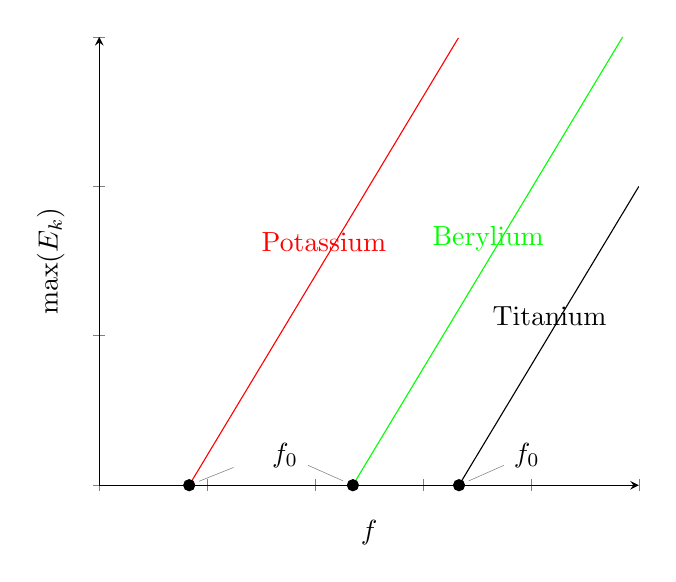
\begin{tikzpicture}
        \begin{axis}[
            axis lines = left,
            xlabel = $f$,
            ylabel = $\max(E_k)$,
            domain=0:10,
            xmin=0, xmax=10, ymin=0, ymax=15,
            yticklabels=\empty,
            xticklabels=\empty,
            samples=300,
        ]
        \addplot[color=red, restrict y to domain=0:15]   {3 * x - 5} node[anchor=east,above,pos=0.5] {\text{Potassium}};
        \addplot[color=green, restrict y to domain=0:15] {3 * x - 14.1} node[anchor=east,above,pos=0.5] {\text{Berylium}};
        \addplot[color=black, restrict y to domain=0:15] {3 * x - 20} node[anchor=east,above,pos=0.5] {\text{Titanium}};
        \addplot[mark=*] coordinates {(5/3,0)} node[pin=15:{}]{};
        \addplot[mark=*] coordinates {(4.7,0)} node[pin=170:{$f_0$}]{};
        \addplot[mark=*] coordinates {(20/3,0)} node[pin=10:{$f_0$}]{};
    \end{axis}
    \end{tikzpicture}
\end{figure}
\FloatBarrier

\begin{definition}{(\textbf{Threshold frequency})}
\textit{The threshold frequency $f_0$ of a photoemissive material is defined as the minimum frequency of the incident radiation which causes photoelectron emissions from the photoemissive surface.}
\end{definition}

Different materials have different threshold frequencies, however most elements (specifically metals) have threshold frequencies in the ultraviolet region of the electromagnetic spectrum.

\begin{definition}{(\textbf{The work function})}
\textit{The work function $\phi$ of a photoemissive material is defined as the minimum energy of the incident photons which causes photoelectron emission from the photoemissive surface.}
\end{definition}

Einstein described these factors using mathematics and the relationship between the maximum kinetic energy $\max(E_k)$ of the photoelectrons and the frequency of the absorbed photons $f$ and the threshold frequency $f_0$ of the photoemissive surface. 
\begin{equation}
    \max(E_k) = h(f - f_0)
\end{equation}
or if you prefer, to the energy of the absorbed photons $E$ and the \textbf{work function} of the surface
\begin{equation}
    \max(E_k) = E - \phi
\end{equation}
where the first term is the energy of the absorbed photons $E$ with frequency $f$ or wavelength $\lambda$ is
\begin{equation*}
    E = hf = \frac{h c}{\lambda}
\end{equation*}
where $c$ denotes the speed of light, and the second term is the \textbf{work function} $\phi$ which is defined as minimum energy required to free a single electron from the surface of the photoemissive surface and is expressed in terms of the threshold frequency $f_0$ of said surface or the threshold wavelength $\lambda_0$
\begin{equation}
    \phi = hf_0 = \frac{hc}{\lambda_0}
\end{equation}

So why did Einstein consider the maximum kinetic energy of the photoelectrons? Some electrons in the surface photoemissive material are closer to positive (metal) ions than others. Their relative positions affect how much energy is required to free them.  The work function is the minimum energy required to free an electron from the photoemissive surface (most electrons require a little more energy than the work function to free them). It follows from the conservation of energy that the electrons that requires the minimum amount of energy for photoemission to occur would have the most energy left from the incident photon. Only a few of the emitted photoelectrons have this \textit{maximum} kinetic energy - which is a fixed value based on the photoemissive material. 

Einstein also noticed a one-to-one interaction between photons and photoelectrons, that is a single incident photon on a photoemissive material with a frequency greater or equal to the threshold frequency of a photoemissive surface will cause a single photoelectron to be emitted. This interaction explains why an increase in intensity increases the rate of photoelectrons emitted. 

\subsection{Wave-particle duality}

The \textbf{wave-particle duality} is a model used to describe how all matter has both wave and particle properties. Electromagnetic radiation is a transverse wave, yet it is also a stream of particles (photons) so it has both wave and particle properties. Louis de Broglie realized that all matter travel through space as waves; matter is built from elementary particles (protons, neutrons, electrons, etc), however, matter is a probability wave (sometimes referred to as a matter wave or a de Broglie wave). 

We normally describe electrons as particles, they have a mass, a charge, can be accelerated, deflected by electric and magnetic fields; all properties we associate with particles. However, under certain conditions an electron can diffract and form a interference pattern in the same way as light. If we use an electron gun to fire an electron at a thin piece of polycrystalline graphite, which has carbon atoms arranged in different layers, the electrons pass between the individual carbon atoms in the graphite.  The gap between the atoms is so small that it is similar to the wavelength of the electrons and so the electrons diffract, as waves and form an interference pattern as seen in figures \ref{fig:electron-gun-electron-diffraction} and \ref{fig:electron-interference}.

\begin{figure}[h!]
    \centering
    \includegraphics[scale=0.1]{notes/images/Wave-Particle.JPG}
    \caption{Electron gun firing electrons at polycrystalline graphite}
    \label{fig:electron-gun-electron-diffraction}
\end{figure}
\FloatBarrier

\begin{figure}[h!]
    \centering
    \includegraphics{notes/images/Electron-Diffraction.JPG}
    \caption{Electron interference pattern}
    \label{fig:electron-interference}
\end{figure}
\FloatBarrier


In developing the wave-particle model, de Broglie combined the following equations to find the wavelength of a particle, 
\begin{equation}
    \vec{p} = m \vec{v} \hspace{1mm} \text{   and   } \hspace{1mm} \| \vec{p} \| = \frac{h}{\lambda} \hspace{0.3cm} \implies \hspace{0.3cm} \lambda = \frac{h}{\| \vec{p} \|} = \frac{h}{m \| \vec{v} \|},
\end{equation}
where $\lambda$ is the wavelength of the particle, $h$ is Planck's constant and $\vec{p}$ is the momentum of the particle. This is known as the \textbf{de Broglie equation}. We can also relate an object's kinetic energy $E_k$ to its wavelength by considering both the de Broglie equation and our general equation for kinetic energy. From the equation above, we have
\begin{equation}
    \lambda = \frac{h}{m \| \vec{v} \|}
\end{equation}
If we can find an expression for $m \| \vec{v} \|$ that includes $E_k$ we can determine the relationship between a particle's kinetic energy and its wavelength. Rearranging the follow relationship
\begin{equation*}
    E_k = \frac{1}{2} m \| \vec{v} \|^2
\end{equation*}
yields, 
\begin{equation}
    m \| \vec{v} \| = \sqrt{2mE_k}.
\end{equation}
We can then substitute this expression into the de Broglie equation, giving
\begin{equation*}
    \lambda = \frac{h}{m \| \vec{v} \|} = \frac{h}{\sqrt{2mE_k}}.
\end{equation*}
As $h$ and $m$ are constants (if we are only concerned with classical mechanics), we can see that the wavelength of a particle is inversely proportional to the square root of it's kinetic energy.
\begin{equation*}
    \lambda \propto \frac{1}{\sqrt{E_k}}.
\end{equation*}

So why don't cars have wavelengths? Do people diffract? The answer lies in the fact that as particles become larger their wave properties become harder to observe. Since
\begin{equation*}
    \lambda \propto \frac{1}{\| \vec{p} \|},
\end{equation*}
as the particle's mass increases, it's momentum increases, so it's wavelength is much smaller, and therefore much harder to observe.

\section{Particle Physics}

\subsection{Rutherford's Alpha-particle Scattering Experiment}

In 1897, English Physicist J.J Thompson discovered the existence of the electron and showed they were smaller than an atom, referred to as a \textit{sub-atomic} particle. Using his discovery, he developed ``plum - pudding'' model of the atom; suggesting that an atom contained negative electrons (the plums) embedded in a uniform sea of positive charge (the dough). 

However, in 1911, Ernest Rutherford and Geiger experimentally showed that the positive charge of the atom existed in a tiny nucleus about $10^{-14}$m in size, thus showing most the atom was empty space. In Rutherford's experiment, a narrow beam of alpha particles, all of the same kinetic energy, from a radioactive source were targeted at a thin piece of gold foil which was only a few atoms thick. The alpha particles were scattered by the foil and detected on a zinc sulfide screen mounted in front of a microscope. Each particle hitting this screen produced a ting flash. The microscope was moved around in order to count the number of alpha particles scattered through different values of the angle $\theta$ per minute.

\begin{figure}[h!]
    \centering
    \includegraphics{notes/images/Rutherford.JPG}
    \caption{Rutherford's Scattering}
\end{figure}
\FloatBarrier

Rutherford concluded the most of the alpha particles passed straight through the gold foil with very little scattering, suggesting that atoms are mainly made of empty space. Furthermore, very few of the alpha particles - about 1 in every 10000 - were deflected through angles greater than $\pi/2$, hence there must be a tiny positive charged called the \textbf{nucleus}. 

In order to be defected at angles greater than $\pi/2$, the scattered alpha particle will momentarily stop a short distance $r$ from the nucleus, before being repelled. Applying the principle of the conservation of energy, we find that
\begin{equation}
    \text{Initial kinetic energy of alpha particle} = \text{Electrical potential energy at distance } r.
\end{equation}
So in this case, we have
\begin{equation}
    \frac{1}{2} m_{\alpha} \| \vec{v} \|^2 = k_e \frac{Q_{gold} Q_{\alpha}}{r}
\end{equation}
Solving for $r$, produces an \textit{upper limit} for the radius of the gold nucleus. More energetic alpha particles might get closer. 

\subsection{The Atom}

We now know that an atom consists of a \textbf{nucleus} containing \textbf{protons} (positively charged particles) and \textbf{neutrons} (particles with a net charge of zero) surrounded by \textit{shells} of \textbf{electrons}. The size of an atom is approximately $10^{-10}$, whereas the size of the nucleus is approximately $10^{-14}$, that is to say the size of an atom is $10000$ times larger than it's nucleus.  

As mentioned previously, the nucleus contains protons and neutrons, which have approximately the same mass. The term \textbf{nucleon} is used to refer to either a proton or a neutron. A proton has the charge of $+e$, where $e$ is the elementary charge. So a neutral atom has the same number of electrons and protons to produce a net charge of zero.

The nucleus of an atom for a particle element is represent as 
\begin{equation}
    _{Z}^A X,
\end{equation}
where $X$ is the chemical symbol of the element, $A$ is the nucleon number (the total number of protons and neutrons) and $Z$ is the proton number (also known as the atomic number). The number of neutrons $N$ in the nucleus is thus $N = A - Z$

\subsubsection*{Isotopes}

\textbf{Isotopes} are nuclei of the same element that have the same number of protons but different numbers of neutrons. All isotopes of an element undergo the same chemical reactions

\subsubsection*{Atomic mass}

The masses of atoms and nuclear particles are often expressed in \textbf{atomic mass units} ($u$). One atomic mass unit $1 u$ is one-twelfth the mass of a neutral carbon-12 atom. 

\subsubsection*{Nuclear Size and Density}

The radius of the nucleus naturally depends on the nucleon number $A$. Recall that fast moving electrons have a de Broglie wavelength about $10^{-15}$. Diffraction of such electrons have be used to empirically prove that the radius $R$ of a nucleus is given by 
\begin{equation}
    R = r_0 A^{1/3},
\end{equation}
where $A$ is the nucleon number and $r_0$ has the approximate value of $1.2$ $fm$ ($1$ $fm = 10^{-15}m$). We now assume that a nucleus is spherical in nature, and therefore it's volume is given by 
\begin{equation}
    V = \frac{4}{3} \pi r_0^3 A
\end{equation}
From the definition of atomic, the mass of any given nucleus is $m = Au$, hence the density of a nucleus is 
\begin{align}
    \rho &= \frac{Au}{\frac{4}{3} \pi r_0^3 A} \\
    &= \frac{3u}{4\pi r_0^3}
\end{align}
Hence the density of any atom is constant.

\subsubsection*{Nuclear Forces}

But if a Nucleus only contains protons and neutrons, what force is overcoming the repulsive electrostatics forces between the protons? The gravitational force between protons is too weak to overcome this force. Therefore there must be another force of attraction, that only acts within the nucleus, known as the \textbf{Strong Nuclear Force}.

This force binds the nucleons together within the nucleus. It acts over a very short range of approximately $10^{-15}$ m. The strong force overcomes the electrostatic repulsion at short range, but becomes repulsive over a long range. 


\begin{figure}[h!]
    \centering
    \includegraphics{notes/images/StrongNuclear5.JPG}
    \caption{Strong Nuclear Force between two neutrons (or a neutron and a proton)}
\end{figure}
\FloatBarrier

\begin{figure}[h!]
    \centering
    \includegraphics{notes/images/StrongNuclear4.JPG}
    \caption{Strong Nuclear Force between two protons}
\end{figure}
\FloatBarrier

The graphs above show that the force is independent of charge and only acts over a range of approximately of 5 fm. The force is powerfully attractive between nucleons at distances of about 1 fm between their centers, but rapidly decreases to insignificance at distances beyond about 3 fm (for neutron and proton interaction) and 4 fm (for proton and proton interaction). At very short distances less than 0.5 fm, it becomes repulsive, and is responsible for the physical size of nuclei, since the nucleons can come no closer than the force allows. Thus preventing the nucleus from collapsing.

\subsection{Antiparticles}
\label{subsection:antiparticles}

In 1928, Paul Dirac invents the relativistic Schodinger equation, known as the Dirac equation. When applied to an electron, the wave equation refers to both an electron with charge $e$ (a positron) and an electron with charge $-e$. From this Dirac predicted that every particle has a corresponding \textbf{antiparticle} which has the same mass, opposite charge and opposite spin. For example, the antiparticle of an electron $e^{-}$ is the positron $e^{+}$. The table below lists some common particles are their corresponding antiparticle;

\begin{table}[h!]
    \centering
    \begin{tabular}{c|c}
        \textit{Particle} & \textit{Antiparticle} \\
        \hline
        \text{proton} $p$ & \text{antiproton} $\overline{p}$ \\
        \text{neutron} $n$ & \text{antineutron} $\overline{n}$ \\
        \text{electron} $e^{-}$ & \text{positron} $e^{+}$ \\
        \text{up quark} $u$ & \text{anti up quark} $\overline{u}$ \\
        \text{down quark} $d$ & \text{anti down quark} $\overline{d}$ \\
        \text{strange quark} $s$ & \text{anti strange quark} $\overline{s}$ \\
        \text{neutrino} $v$ & \text{anti neutrino} $\overline{v}$ \\
    \end{tabular}
\end{table}
\FloatBarrier

Dirac also theorised that if a particle meets it's antiparticle they \textbf{annihilate} where the masses of both particle and antiparticle are converted into a high-energy pair of photons. For example,
\begin{equation}
    e^- + e^+ \longrightarrow 2 \gamma
\end{equation}
In order to conserve momentum, the 2 photons will travel in opposite directions. 

\begin{figure}[h!]
    \centering
    \includegraphics[scale=0.15]{notes/images/Annihilation.JPG}
    \caption{Electron and Positron annihilation}
\end{figure}
\FloatBarrier

\textbf{Pair production} is the opposite process to annihilation, where high energy photons create a particle-antiparticle pair. 

\subsection{Quarks}

In 1963, American physicist Murrary Gell-Mann performed the deep inelastic scattering experiment. Gell-Mann postulated that nucleons contained particles called \textbf{Quarks}. In order to discover the structure of nucleons, electrons were fired at them in a similar experiment to Rutherford's alpha-particle scattering experiment. The results showed the existence of three concentrations of mass and charge within the nucleon, implying that a nucleon consisted of three quarks. 

The standard model of elementary particles requires six quarks and six anti-quarks. The six quarks are up, down, charm, strange, top and bottom denoted by $u, d, c, s, t$ and $b$, respectively. All quarks have a charge that is a fraction of the elementary charge $e$ (the only case where charge isn't quantized).

All the quarks are listed in the table below, but for A2 Physics we only need to use up, down and strange quarks and their anti-quarks. 

\begin{table}[h!]
    \centering
    \begin{tabular}{c | c c c c}
        \textit{Quark} & \textit{Symbol} & \textit{Relative Charge*} & \textit{Baryon Number} & \textit{Strangeness}\\
        \hline
        \text{up} & $u$ & $+\frac{2}{3}$ & $\frac{1}{3}$ & $0$ \\[2mm]
        \text{down} & $d$ & $-\frac{1}{3}$ & $\frac{1}{3}$ & $0$\\[2mm]
        \text{charm} & $c$ & $+\frac{2}{3}$ & $\frac{1}{3}$ & $0$ \\[2mm]
        \text{strange} & $s$ & $-\frac{1}{3}$ & $\frac{1}{3}$ & $-1$\\[2mm]
        \text{top} & $t$ & $+\frac{2}{3}$ & $\frac{1}{3}$ & $0$ \\[2mm]
        \text{bottom} & $b$ & $-\frac{1}{3}$ & $\frac{1}{3}$ & $0$
    \end{tabular}
\end{table}
\FloatBarrier

\begin{table}[h!]
    \centering
    \begin{tabular}{c | c c c c}
        \textit{Anti-quark} & \textit{Symbol} & \textit{Relative Charge*} & \textit{Baryon Number} & \textit{Strangeness}\\
        \hline
        \text{anti up} & $\overline{u}$ & $-\frac{2}{3}$ & $-\frac{1}{3}$ & $0$ \\[2mm]
        \text{anti down} & $\overline{d}$ & $+\frac{1}{3}$ & $-\frac{1}{3}$ & $0$\\[2mm]
        \text{anti charm} & $\overline{c}$ & $-\frac{2}{3}$ & $-\frac{1}{3}$ & $0$ \\[2mm]
        \text{anti strange} & $\overline{s}$ & $+\frac{1}{3}$ & $-\frac{1}{3}$ & $1$\\[2mm]
        \text{anti top} & $\overline{t}$ & $-\frac{2}{3}$ & $-\frac{1}{3}$ & $0$ \\[2mm]
        \text{anti bottom} & $\overline{b}$ & $+\frac{1}{3}$ & $-\frac{1}{3}$ & $0$
    \end{tabular}
\end{table}
\FloatBarrier

\noindent * relative to the elementary charge. 

\subsubsection*{Strangeness}

If a particle contains a strange quark it is said to be a \textbf{strange} particle. Strange particles are unusually long lived. The ``strangeness'' value of a particle lies in the range $[-3, 3]$. In all interactions containing strong nuclear force, strangeness is conserved. However, in weak interactions, the strangeness value may change by $-1, 0$ or $+1$. 

\subsection{Fundamental and Non-Fundamental Particles}

\noindent All particles are split into two families - fundamental particles and non-fundamental particles. 
\begin{itemize}
    \item \textbf{Fundamental Particles}: Particles with no internal structure that cannot be broken down into smaller constituents. Examples include Quarks (see above), Leptons and Exchange particles:
    \begin{itemize}
        \item \textbf{Leptons}: Leptons are particles and antiparticles that are not affected by the strong nuclear forces. Examples include electrons, muons, taus and neutrinos. All leptons have a lepton number of $1$ and all anti-leptons have a lepton number of $-1$. In all particle interactions, the lepton number must be conserved.  
        \item \textbf{Exchange particles}: Exchange particles are virtual particles that mediate the interaction between two other particles. Examples include gluons and photons. 
    \end{itemize}
    \item \textbf{Non-Fundamental Particles}: In A2 Physics, all non-fundamental particles are \textbf{Hadrons} which are made from quarks. \textbf{Hadrons} are particles and antiparticles that are affected by strong nuclear forces. Examples include protons, neutrons (baryons), pions and kaons (mesons)
    \begin{itemize}
        \item \textbf{Baryons}: Baryons are particles and antiparticle consisting of \textbf{three quarks}. Protons and neutrons are baryons, with the following quark compositions 
        \begin{equation*}
            p = uud \text{ and } n = udd.
        \end{equation*}
        Anti-protons and anti-neutrons are anti-baryons with the following quark compositions
        \begin{equation*}
            \overline{p} = \overline{u}\overline{u}\overline{d} \text{ and } \overline{n} = \overline{u}\overline{d}\overline{d}.
        \end{equation*}
        All baryons have a baryon number of $1$ and all anti-baryons have a baryon number of $-1$. In all particle interactions, the baryon number must be conserved.
        \item \textbf{Mesons}: Mesons are particles and antiparticles consisting of a quark and a anti-quark pair. For example, the meson known as a pion denoted by $\pi^0, \pi^+$ has the following quark composition:
        \begin{equation*}
            \pi^0 = u \overline{u} \text{ or } \pi^0 = d \overline{d} \text{ and } \pi^+ = u \overline{d}  
        \end{equation*}
        The anti-pion (an anti-meson) is $\pi^0$ and $\pi^-$, so 
        \begin{equation*}
            \overline{\pi^0} = \pi^0 \text{ and } \overline{\pi^+} = \pi^- = \overline{u} d
        \end{equation*}
        The Kaon $K$ is meson and a strange particle (with a strangeness of $1$), with the following quark composition
        \begin{equation*}
            K^0 = d \overline{s} \text{ and } K^+ = u \overline{s}
        \end{equation*}
        The anti-kaon is an anti-meson with a strangeness of $-1$ with the following compositions
        \begin{equation*}
            \overline{K^0} = K^0 \text{ and } \overline{K^+} + K^- = \overline{u} s.
        \end{equation*}
    \end{itemize}
\end{itemize}

\noindent Note that in all particle interactions, four quantities are conserved:
\begin{itemize}
    \item Charge
    \item Baryon Number
    \item Lepton Number
    \item Strangeness 
\end{itemize}

\subsection{Beta Decay}

There are various types of radiation that unstable nuclei emit, such as $\alpha$, $\beta$ and $\gamma$. We will discuss these types of radiations in more detail in section ??.

Beta decays is the emission of either electrons $\beta^-$ decay, or positrons $\beta^+$ decay. These emissions must be related to changes taking place within the nuclei of the atoms. In the case of beta day, the changes occur to the neutrons or the protons. The force responsible for beta decay is the \textbf{weak nuclear force}. The weak nuclear force acts between quarks in the nucleus and leptons. The weak force has a very short range, approximately $10^{-18}$ m.

In $\beta^-$ decay, a neutron $_0^1 n$ in an unstable nucleus decays into a proton $_1^1 p$, an electron $_{-1}^0 e$ and an electron anti-neutrino $\overline{v_e}$. 
\begin{equation}
    _0^1 n \longrightarrow \hspace{1mm} _1^1 p + _{-1}^{0} e + _0^0 \overline{v_e} + \text{energy}
\end{equation}


In $\beta^+$ decay, a proton $_1^1 p$ in an unstable nucleus decays into a neutron $_0^1 n$, a positron $_{1}^0 e$ and an electron neutrino $v_e$. 
\begin{equation}
    _1^1 p \longrightarrow \hspace{1mm} _0^1 n + _{1}^{0} e + _0^0 v_e + \text{energy}
\end{equation}

Since protons and neutrons consist of quarks; each type of beta decay is associated with the decay of a specific quark within the proton or the neutron. In $\beta^-$ decay one of the down quarks changes \textbf{flavour} to an up quark, so the decay equation is
\begin{equation}
    d \longrightarrow \hspace{1mm} u + _{-1}^{0} e + _0^0 \overline{v_e} + \text{energy}
\end{equation}

Similarly, in $\beta^+$ decay, one of the up quarks changes \textbf{flavour} to a down quark, hence 

\begin{equation}
    u \longrightarrow \hspace{1mm} d + _{1}^{0} e + _0^0 v_e + \text{energy}
\end{equation}

\section{Nuclear Physics}

\subsection{Radioactive Decay}

Radioactive decay is a process whereby a nucleus attempts to stabilise itself by releasing energy through radiation. A negligible amount can be detected in nature, and this is called \textbf{background radiation}, a large proportion of which is radon gas resultant from the decay of uranium within rocks. \textbf{Activity} is the measure of rate of radioactive decay, with unit \textbf{Becquerel}. 

Say \(N\) is the number of undecayed nuclei in a sample. While \(N\) is obviously discrete, being a natural number, it is often large enough to be well-approximated as a continuous variable. While, it is a random process, it is impossible to predict when any undecayed nuclei may decay, (and if we are to treat \(N\) as continuous variable, the probability of decay in any particular instant is zero) we can suppose it is equally likely that undecayed nuclei will decay in one instant than any other. 

As \(N\) is a continuous quantity dependent on \(t\), it makes sense to take a derivative in the usual sense. 

\begin{definition}{(\textbf{Activity})}
\textit{We define the activity of a sample at time \(t_0\) as:}

\begin{equation}
A(t = t_0) = \left. \frac{\mathop{\mathrm{d} N}}{\mathop{\mathrm{d} t}} \right|_{t = t_0}
\end{equation}
\end{definition} 

We know that the likelihood of decay at any given time will be proportional to the number of remaining undecayed nuclei at that instant, since we supposed that each have an equal probability of decaying in that instant. We can therefore write 
\begin{equation}
A \propto N
\end{equation}

As the activity of the sample will decrease with time, we expect the constant of proportionality here to be negative. Write this constant of proportionality \(-\lambda\), and we call \(\lambda\) the \textbf{decay constant}. Then we have the following differential equation 
\begin{equation}
\frac{\mathop{\mathrm{d} N}}{\mathop{\mathrm{d} t}} = -\lambda N.
\end{equation} 
If the initial number of undecayed nuclei is \(N_0\), we should require that \(N = N_0\) at \(t=0\).  Which can trivially be solved by the separation of variables: 
\begin{align} 
\frac 1 N \frac{\mathop{\mathrm{d} N}}{\mathop{\mathrm{d} t}} &= -\lambda \\ 
\int_{N_0}^N \frac {\mathop{\mathrm{d} N}} N &= -\lambda \int_0^t \mathop{\mathrm{d} t} \\ 
\ln \left | \frac{N}{N_0} \right| &= -\lambda t 
\\ N &= N_0 \exp(-\lambda t)
\end{align}
Hence, activity can then be determined by taking the derivative of the $N$ 
\begin{equation} 
A = \frac{\mathop{\mathrm{d} N}}{\mathop{\mathrm{d} t}} = -\lambda N_0 \exp(-\lambda t)
\end{equation} 

As we have defined the activity of the sample as being \(-\lambda N\) at any instant, the initial activity of the sample \(A_0\) is equal to \(-\lambda N_0\) where \(N_0\) is the initial number of undecayed nuclei. With that we may rewrite the original equation as 
\begin{equation} 
A = A_0 \exp(-\lambda t)
\end{equation} 

We may be interested in ways to calculate the decay constant. A common measure of the radioactivity of a substance is its half-life: 

\begin{definition}{(\textbf{Half-Life})}
\textit{The \textbf{half-life} of a particular the sample is the length of time it takes for half of the unstable nuclei in the sample to decay.}
\end{definition} 

We can determine this using, for example, the graph of the activity of the sample against time (which we could produce electronically with aid of a GM counter). We can then use this to then determine the decay constant \(\lambda\). Let use denote the half-life of a particular sample as \(t_{1/2}\), and its initial undecayed nuclei count as \(N_0\). At \(t_{1/2}\), the count of undecayed nuclei is \(\frac 1 2 N_0\), so
\begin{equation} 
\frac{N_0} 2 = N_0 e^{-\lambda t_{1/2}}
\end{equation} 
Dividing through by \(N_0\) and taking the natural log of both sides
\begin{equation*}
\ln \frac 1 2 = -\lambda t_{1/2}
\end{equation*} 
writing \(\ln \frac 1 2 = -\ln 2\), we have
\begin{equation} 
\lambda = \frac {\ln 2} {t_{1/2}}.
\end{equation} 

\subsection{Radioactive decay processes}
We have spoke a lot about the rate at which nuclei decay, but we have not yet discussed the processes by which they decay. 

\textbf{\(\alpha\) decay} occurs when a nuclei has too many protons compared to the number of neutrons. This causes the nucleus to eject a helium-4 atom, comprised of 2 protons and 2 neutrons as to reduce the ratio between protons and neutrons. This type of radiation can pose significant danger, as it is strongly ionising and can therefore cause serious damage if put into contact with, for example, internal organs. (if an alpha admitter is accidentally consumed) However, as it is so ionising, it quickly loses kinetic energy and can therefore be easily absorbed. It is absorbed by a few centimetres of air or a sheet of paper. An example of an \(\alpha\) decay process is: 

\begin{equation*} 
_{95}^{241} \textrm{Am} \longrightarrow \hspace{1mm} _{93}^{237} \textrm{Np} + _2^4 \alpha
\end{equation*} 

\textbf{\(\beta^-\) decay} occurs when there a nuclei has too many neutrons compared to the number of protons. This causes a neutron to decay into a proton (by changing its quark configuration) and an electron, (which we call a \(\beta\) particle) which is ejected along with an antineutrino. The \(\beta\) particle has half the charge of an \(\alpha\) particle and is much smaller, so is less ionising. But with this, it loses kinetic energy at a slower rate, and so can penetrate further. A thin sheet of aluminium is usually sufficient to absorb a \(\beta\) particle. 

\begin{equation*} 
_{6}^{14} \textrm{C} \longrightarrow \hspace{1mm} _{7}^{14} \textrm{N} + _{-1}^{0} \beta + _{0}^{0} \overline{v}
\end{equation*} 

\textbf{Gamma decay} occurs when a massive nuclei has too much energy, usually occurring immediately after \(\alpha\) or \(\beta\) decay as the nucleus is left in an excited state. Unlike the other types of decay, this does not release any particles and hence does not change the nuclei in any way. Instead, gamma rays are high frequency electromagnetic waves. As they are EM waves and not particles, they do not have mass or charge, so will rarely interact. However, this means that they are extremely difficult to absorb, and can only be absorbed by several inches of lead or several metres of concrete. This means that gamma is most often considered the most dangerous radiation.  

\subsection{Relativity and Einstein's Mass-Energy Equation}

Let us consider momentum in both Classical and Relativistic mechanics. In both models, momentum is defined as 
\begin{equation}
    \vec{p} = m \vec{v},
\end{equation}
and momentum is conserved in a closed system, that is 
\begin{equation}
    \frac{\mathop{\mathrm{d}}}{\mathop{\mathrm{d}t}} \sum \vec{p} = 0
\end{equation}
However, in a classical model we have
\begin{equation}
    \lim_{\vec{v} \rightarrow \infty} \vec{p} = \infty    
\end{equation} 
This is not allowed in special relativity, hence we redefine mass so it has a velocity dependence, 
\begin{equation}
    m = m_0 f(v).
\end{equation}
such that $f(v = 0) = 1$. In fact
\begin{equation}
    m = m_0 \gamma = \frac{m_0}{\sqrt{1 - v^2 / c^2}},
\end{equation}
where $c$ is the speed of light in a vacuum. So we have
\begin{equation}
    \vec{p} = \frac{m_0 \vec{v}}{\sqrt{1 - v^2 / c^2}},
\end{equation}
where $m_0$ is the \textbf{rest mass}. So in a relativistic model, Newton's second law of motion for a single particle of rest mass $m_0$ becomes
\begin{align}
    \vec{F} &= \frac{\mathop{\mathrm{d}\vec{p}}}{\mathop{\mathrm{d}t}} \\
    &= m_0 \frac{\mathrm{d}}{\mathop{\mathrm{d}t}} \gamma \vec{v} \\
    &= m_0 \left(\gamma \vec{a} + \vec{v} \frac{\mathop{\mathrm{d}\gamma}}{\mathop{\mathrm{d}t}}\right)
\end{align}
We will now consider the relativistic kinetic energy of the particle, by considering the work done by $\vec{F}$. So by definition, we have
\begin{equation}
    W = \int_C \vec{F} \cdot \mathop{\mathrm{d}\vec{r}}
    \label{eq:sr-work-1}
\end{equation}
To simplify the model, we will consider motion in one-dimension, allowing us to replace the line integral with a regular integral. Also, note that $\mathop{\mathrm{d}\vec{r}} = \vec{v} \mathop{\mathrm{d}t}$. Applying this to equation \ref{eq:sr-work-1} gives us
\begin{equation}
    W = \int_0^t m_0 v \left(\gamma \frac{\mathop{\mathrm{d}v}}{\mathop{\mathrm{d}t}} + v \frac{\mathop{\mathrm{d}\gamma}}{\mathop{\mathrm{d}t}}\right) \mathop{\mathrm{d}t}.
    \label{eq:sr-work-2}
\end{equation}
Let us now consider the time derivative of gamma, 
\begin{align}
    \frac{\mathop{\mathrm{d}\gamma}}{\mathop{\mathrm{d}t}} &= \frac{\mathrm{d}}{\mathop{\mathrm{d}t}} \frac{1}{\sqrt{1 - v^2/c^2}} \\
    &= - \frac{1}{2} (1 - v^2 / c^2)^{-\frac{3}{2}} \left(-\frac{2v}{c^2} \frac{\mathop{\mathrm{d}v}}{\mathop{\mathrm{d}t}}\right) \\
    &= v \frac{\gamma^3 }{c^2} \frac{\mathop{\mathrm{d}v}}{\mathop{\mathrm{d}t}} \label{eq:sr-dgamma-1}
\end{align}
Substituting the above expression into equation \ref{eq:sr-work-2} gives
\begin{align}
    W &= \int_0^t m_0 v \left(\gamma \frac{\mathop{\mathrm{d}v}}{\mathop{\mathrm{d}t}} + \gamma^3 \frac{v^2}{c^2} \frac{\mathop{\mathrm{d}v}}{\mathop{\mathrm{d}t}}\right) \mathop{\mathrm{d}t} \\
    &= \int_0^t m_0 v \gamma \frac{\mathop{\mathrm{d}v}}{\mathop{\mathrm{d}t}} \left(1 + \frac{v^2}{c^2} \gamma^2\right) \mathop{\mathrm{d}t}
\end{align}
Considering the 5$^{th}$ term of the integrand above gives
\begin{align}
    1 + \frac{v^2}{c^2} \gamma^2 &= 1 + \frac{v^2}{c^2} \frac{1}{1-v^2/c^2} \\
    &= \frac{1-v^2/c^2+v^2/c^2}{1-v^2/c^2} \\ 
    &= \gamma^2
\end{align}
Hence the work done is 
\begin{equation}
    W = \int_0^t m_0 v \gamma^3 \frac{\mathop{\mathrm{d}v}}{\mathop{\mathrm{d}t}} \mathop{\mathrm{d}t}. 
\end{equation}
Rearranging equation \ref{eq:sr-dgamma-1} yields
\begin{equation}
    c^2 \frac{\mathop{\mathrm{d}\gamma}}{\mathop{\mathrm{d}t}} = v \gamma^3 \frac{\mathop{\mathrm{d}v}}{\mathop{\mathrm{d}t}}
\end{equation}
Applying this to the expression for work done above, we find that 
\begin{align}
    W = \int_0^t m_0 c^2 \frac{\mathop{\mathrm{d}\gamma}}{\mathop{\mathrm{d}t}} \mathop{\mathrm{d}t} 
\end{align}
Suppose the particle we're considering is at rest at time $t = 0$, so we have
\begin{align}
    W &= m_0 c^2 \int_1^\gamma \mathop{\mathrm{d}\gamma} \\
    &= m_0 c^2 (\gamma - 1)
\end{align}
This is the expression for \textbf{Relativistic kinetic energy} $E_{k,r}$. It follows that for small $v^2/c^2$, we have
\begin{equation}
    \sqrt{1 - \frac{v^2}{c^2}} \approx 1 - \frac{1}{2}\frac{v^2}{c^2}.
\end{equation}
So 
\begin{align}
    E_{k,r} &= m_0 c^2 \left(\frac{1}{1-v^2/2c^2} - 1\right) \\
    &= m_0 c^2 \frac{v^2}{2c^2} \\
    &= \frac{1}{2} m_0 v^2
\end{align}
The classical equation for kinetic energy!. Now let us define the energy $E$ of the particle as 
\begin{equation}
    E = E_{k,r} + m_0 c^2 = \gamma m_0 c^2.
\end{equation}
Now consider $E^2 - (pc^2)$, where $p$ is the momentum of the particle (in our one-dimension model). So we have
\begin{align}
    E^2 - (pc)^2 &= m_0^2 c^4 \gamma^2 - \gamma^2 m_0^2 c^2 v^2 \\
    &= (m_0c)^2 \gamma^2 (c^2 - v^2).
\end{align}
However, recall that
\begin{equation}
    \gamma^2 = \frac{1}{1-v^2/c^2} = \frac{c^2}{c^2 - v^2},
\end{equation}
then
\begin{equation}
    E^2 - (pc)^2 = (m_0c^2)^2
\end{equation}
Now when the particle is at rest, i.e $v = 0$, we have
\begin{equation}
    E = m_0 c^2.
\end{equation}
Einstein's mass-energy equation! The interpretations of this equation are
\begin{itemize}
    \item Firstly, mass is a form of energy. The interaction of a particle and it's anti particle, known as \textbf{annihilation}, is an example of this (see section \ref{subsection:antiparticles}).
    \item Alternatively, we could say energy has mass. This is similarly demonstrated by \textbf{pair production} (see section \ref{subsection:antiparticles})
\end{itemize}  

\subsection{Einstein's mass-energy equation and Binding energy}
\begin{definition}{(\textbf{Atomic mass unit})} 
\textit{We define \(u\) to be \(\frac 1 {12}\)th of the mass of a carbon-12 atom. \(u \approx 1.67 \times 10^{-27} \textrm{kg}\) to 3 s.f.}
\end{definition} 

The mass of a nucleon is then about \(1u\). While we would expect the mass of a nucleus to be given by the sum of the masses of its constituent nucleons, this is not the case. The measured mass will always be less than this. The difference between these two masses is the \textbf{mass deficit}. This deficit is caused because a small amount of the mass is converted to \textbf{binding energy} - which is needed to hold the nucleus together. 

\begin{definition}{(\textbf{Binding energy})}
\textit{We define the binding energy $E_b$ of a nucleus as the minimum energy required to completely separate a nucleus into its constituent nucleons.}
\end{definition}
\begin{definition}({\textbf{Mass deficit}})
\textit{We define the mass deficit $\Delta m$ as the difference between the mass of the completely separated nucleons and the mass of the nucleus.}
\end{definition}

The binding energy $E_b$ can be calculated using Einstein's mass-energy equation: 
\begin{equation*}
E_b = c^2 \Delta m
\end{equation*} 

where \(E_b\) is the required binding energy, \(c\) is the speed of light in a vacuum and \(\Delta m\) is the mass deficit. Due to the comparatively low mass of electrons compared to the other nucleons, they are often ignored in calculations of mass. 

\begin{example}
For example, take a carbon-\(12\) atom, which has 6 protons (with mass \(\approx 1.008665u\)) and 6 neutrons (with mass \(\approx 1.007276u\)). From the definition of \(u\), this atom has mass \(12u\), so the mass deficit is approximately \((12 - 6 \cdot 1.008665 - 6 \cdot 1.007276)u = - 0.098937u\), giving a binding energy of approximately \(92.3 \textrm{MeV}\). 
\end{example}
\begin{example}
Consider a uranium-$235$ atom, which has $92$ protons and $143$ neutrons. Therefore the mass of the nucleons are $(92 \times 1.007276u) + (143 \times 1.008665u) = 236.908487u$. Given the mass of the nucleus is $235.004393u$, then the mass deficit is 
\begin{align}
    \Delta m &= (235.004393 - 236.908487)u = - 1.904094 u\\ 
    &= - 1.904094 \times 1.661 \times 10^{-27}\\ 
    &= - 3.162700 \times 10^{-27} \text{ kg}.
\end{align}
So the binding energy of the nucleus is 
\begin{align}
    E_b &= 3.162700 \times 10^{-27} \times (3 \times 10^8)^2 \\
    &= 2.846430 \times 10^{-10} \text{ J} \\
    &= 1779 \text{ MeV}.
\end{align}
\end{example}

We may be interested in how much energy it takes to remove a nucleon from an atom. If more energy is required to remove a nucleon from the nucleus, we can conclude that the nucleus is more "tightly bound" and hence harder (ie. requires more energy) to break apart. To quantify this we take the \textbf{binding energy per nucleon}, by dividing the mass by the number of nucleons. (we are merely taking an average, so the difference in mass between protons and neutrons does not matter.)  

\begin{figure}[h!]
    \centering
    \includegraphics[scale=0.75]{notes/images/BE-Per-Nucleon.JPG}
    \caption{Binding energy per nucleon against nucleon number $A$ for nuclei}
    \label{fig:be-per-nucleon}
\end{figure}
\FloatBarrier

The figure above shows the binding energy per nucleon against nucleon number $A$. Some deductions can be made about radioactive decay, nuclear fission and fusion from the graph;
\begin{itemize}
    \item For nuclei with $A < 56$, the binding energy per nucleon increases as $A$ increases.
    \item For nuclei with $A > 56$, the binding energy per nucleon decreases as $A$ increases.
    \item $_{26}^{56}$Fe has the greatest binding energy per nucleon and is the most stable isotope in nature.
    \item $_{2}^4$He nuclei has an abnormally greater binding energy per nucleon than it's neighbours. $_6^{12}$C and $_8^{16}$O also exhibit this property.
    \item In radioactive decay, the graph shows the total binding energy of the parent nucleus is less than the binding energy of the daughter nucleus and the alpha particle. The extra energy is released as kinetic energy.
    \item In a nuclear fission reaction, a nucleus with a high $A$ splits into lower $A$ number nuclei. Energy is released because the two daughter nuclei have higher binding energies than the parent nucleus. 
    \item In a nuclear fusion reaction, two low $A$ number nuclei amalgamate to form a higher $A$ number nucleus, which has a much greater binding energy than the initial nuclei and therefore energy is released. 
    
\end{itemize}
\subsection{Fission}
Nuclear fission is the splitting of a heavy nucleus into lighter daughter nuclei. These lighter daughter nuclei have a greater binding energy per nucleon than that of the heavy nucleus, so the sum of the masses of the daughter nuclei is less than that of the larger nucleus. Due to mass-energy conservation, this releases energy equal to \(E = c^2 \Delta m\). 

The need for heavier nuclei can be seen in Figure \ref{fig:be-per-nucleon}, as beyond iron-56, the binding energy per nucleon decreases as nucleon number increases, so performing fission with nuclei sufficiently heavier than iron causes the desired effect.  

Uranium is the most common fuel used in nuclear fission. The uranium-235 isotope easily undergoes fission on absorbing a slow neutron, known as a \textbf{thermal neutron} (because their mean kinetic energy is similar to the thermal energy of the particles in the reactor core). A typical induced fission reaction of uranium-235 by a thermal neutron is
\begin{equation}
    _{92}^{235}\text{U} + _0^1\text{n} \longrightarrow \hspace{1mm} _{92}^{236}\text{U} \longrightarrow \hspace{1mm} _{56}^{141}\text{Ba} + _{36}^{92}\text{Kr} + 3 \hspace{1mm} _{0}^1\text{n}.
\end{equation}
The uranium-235 nucleus captures the neutron, becomes a highly unstable nucleus of uranium-236. The uranium-236 nucleus than splits, the daughter nuclei produced in the example above are barium-141 and krypton-92. Three fast neutrons are also produced. 

\subsubsection*{Chain Reactions}

If the three fast neutrons discussed above could be slowed, they could induce further fission reactions. This causes a \textbf{nuclear chain reaction}.

\begin{definition}{(\textbf{Nuclear Chain Reaction})}
\textit{A nuclear chain reaction is series of nuclear reactions, each initiated by the preceding nuclear reaction.}
\end{definition}

In a nuclear fission chain reaction, the \textbf{mean generation time} $\Lambda$ is the average time from a neutron emission to a capture that results in fission. 

\begin{equation}
    \Lambda = \frac{l}{k},
\end{equation}
where $l$ is the neutron life time and $k$ is the effective neutron multiplication factor, described below. 

The neutron multiplication factor $k$ is the average number of neutrons from one fission that induce another fission. We can consider how $k$ determines how a nuclear chain reaction proceeds. Firstly, we note that the following differential equation used to model a nuclear chain reaction (note that I am unsure about the validity of this relationship, as I derived it using a thought experiment).
\begin{equation}
    \frac{\mathop{\mathrm{d}N}}{\mathop{\mathrm{d}t}} = \frac{k-1}{\tau} N - \kappa N,
\end{equation}
where $\tau$ is the mean time for one cycle and $\kappa$ is to account for some inhibitors. If the initial number of neutrons is $N_0$. We can solve the differential equation by the separation of variables
\begin{align}
    \frac{1}{N} \frac{\mathop{\mathrm{d}N}}{\mathop{\mathrm{d}t}} &= \frac{k-1}{\tau} - \kappa \\
    \int_{N_0}^N \frac{\mathop{\mathrm{d}N}}{N} &= \left(\frac{k-1}{\tau} - \kappa\right) \int_0^t \mathop{\mathrm{d}t} \\
    \ln\left|\frac{N}{N_0}\right| &= \left(\frac{k-1}{\tau} - \kappa\right) t\\
    N &= N_0 \exp\left(\left[\frac{k-1}{\tau} - \kappa\right]t\right) 
\end{align}
\begin{example}
So for example, suppose we consider the number of neutrons in a reaction with an effective neutron multiplication factor of $k = 1.01$, a cycle time of $\tau = 0.001$s with no inhibitors (hence $\kappa = 0$) after one second has elapsed;
\begin{equation}
    \frac{N}{N_0} = e^{0.01/0.001} = e^{10}
\end{equation}
So it is clear that $k>1$, we have an exponential increase in neutrons.
\end{example}
\noindent So the value of $k$ determines how the nuclear reaction proceeds
\begin{itemize}
    \item $k<1$: \textbf{Subcriticality}: The system cannot sustain a chain reaction, and any beginning of a chain reaction dies out over time.
    \item $k = 1$: \textbf{Criticality}: Every fission causes an average of one more fission, leading to a fission level that is constant. This is optimal for a nuclear power plant (provided inhibitors are minimised).
    \item $k > 1$: \textbf{Supercriticality}: For every fission reaction, it is likely that there will be $k$ fissions after the next mean generation time. The number of fissions reactions increases exponentially, according to the equation
    \begin{equation}
        \text{number of reactions} = e^{(k-1)t/\Lambda},
    \end{equation}
    where $t$ is the elapsed time. 
\end{itemize}

\subsubsection*{Fission Reactors}

Firstly, we note that a uranium reactor will \textbf{never} explode even if it goes supercritical. As the reactor core heats up, the kinetic energy of the thermal neutrons increases, thus decreasing the number of fission reactions (as slow moving neutrons are required to induce a reaction). So the reaction stabilises at a high temperature, however this leads to a \textbf{MELTDOWN}. A meltdown is where the nuclear material in the reactor melts (\textit{pretty self explanatory really...}).

\begin{figure}[h!]
    \centering
    \includegraphics[scale=0.75]{notes/images/Reactor.JPG}
    \caption{Nuclear Reactor Design.}
\end{figure}
\FloatBarrier

In this course, we'll consider the a common fission reactor design, known as a \textbf{Thermal reactor} (see figure above). 
%a thermal reactor makes uses of delayed neutron emission by designing the reactor to be subcritical to prompt neutrons and use the delayed neutrons to take it to critical. So following a nuclear fission reaction, the fast prompt neutrons are removed. They are then thermalized (increase the thermal energy of the neutron) and allow them to drift back into the fuel. 
The \textbf{fuel rods} in a reactor are spaced evenly in a steel-concrete vessel known as the \textbf{core}. A \textbf{coolant} removes the thermal energy produced by the fission reactions. The fuel rods are surrounded by the \textbf{moderator}, and \textbf{control rods}. The \textit{fuel rods} consist of enriched uranium, mainly uranium-238 and a small amount of uranium-235. The \textit{moderator} slows down the neutrons produced by nuclear fission reactions. The mean kinetic energy of the thermal neutrons $\overline{E_k}$ is given by
\begin{equation}
    \overline{E_k} = \frac{3}{2}kT,
\end{equation}
where $T$ is the thermodynamic temperature of the core. When a fast moving neutron collides elastically with protons in water or with carbon nuclei, they transfer significant kinetic energy and slow down. Suggesting water and carbon are good moderators. Many reactors uses water as both a moderator and a coolant. The \textit{control rods} are designed to absorb the neutrons, most commonly boron or cadmium. The position of the control rods is adjusted to ensure that the reactor maintains criticality. 

Nuclear fission reactors produce extremely hazardous materials such as Plutonium-239. Radioactive waste from reactors must be buried deep underground for many centuries because the isotopes with long half lives (for example 24 thousand years) must not enter water and food supplies. These burial locations need to be geologically stable, secure from attack, and designed by safety. 

\subsection{Fusion}
Nuclear fusion is the fusing of two lighter nuclei to form a heavier nucleus. Identically to fission, this heavier nucleus has a higher binding energy per nucleon, (hence why light nuclei is used, referring back to figure \ref{fig:be-per-nucleon}) so energy is released due to mass-energy conservation. 

For a given mass of reactant, fusion produces the most energy, though due to the conditions required for fusion to occur, a fusion reactor on Earth is unviable. For example, in a proton-proton fusion reaction, there is a strong electrostatic force of repulsion between the two protons (as they are like charges) that prevents the two particles from interacting. High temperatures would have to be used to give the particles enough kinetic energy to overcome this repulsion, to become close enough to interact. Similarly, to maintain a sufficiently high collision rate for the process to produce a viable amount of energy, high densities are required. 

As seen in the astrophysics chapter, fusion occurs inside stars, and the amount of fusion occurring throughout the star (determined by its power output) is indicative of the stage that the star is through its life-cycle. In this case the above conditions for viability are satisfied due to the massive gravitational forces present inside the star. 

Here are some common nuclear fusion reactions
\begin{itemize}
    \item Two protons fuse to produce a deuterium nucleus, a positron and a electron neutrino. 
    \begin{equation}
        2 \hspace{1mm} _1^1 \text{p} \longrightarrow \hspace{1mm} _1^2\text{H} + _1^0 \text{e} + v_e
    \end{equation}
    Produces $2.2$ MeV.
    \item A deuterium nucleus and a proton fuse, producing a helium-3 nucleus
    \begin{equation}
        _1^2\text{H} + _1^1\text{p} \longrightarrow \hspace{1mm} _2^3\text{He}
    \end{equation}
    Produces $5.5$ MeV.
    \item Two helium-3 nuclei fuse, producing a helium-4 nucleus and two protons
    \begin{equation}
        2 _2^3\text{H} \longrightarrow \hspace{1mm} _2^4\text{He} + 2_1^2\text{p}
    \end{equation}
    Produces $12.9$ MeV.
\end{itemize}

Notice the series of reactions produces a self sufficient cycle (provided there is enough energy in the system). 

\section{Medical Physics}

\subsection{X-Rays}

\subsubsection*{Nature}
\begin{itemize}
    \item X-rays can be polarised, diffracted by atoms in crystals and have extremely short wavelengths.
    \item They are electromagnetic waves.
    \item X-ray photons have 10-10,000 more energy than a visible light photon, depending on their wavelength.
    \item X-rays are harmful to living cells. Commonly used in the treatment of cancer cells.
\end{itemize}

\subsubsection*{Production}
\begin{itemize}
    \item Produced when fast-moving electrons are deceleration by interaction with atoms of a metal. The kinetic energy of the electrons is transformed into x-ray photons.
    \item X-ray machines contain an x-ray tube that produces x-ray photons that pass through the patient to the detection plate below. \textbf{Digital detection} plates have replaced photographic plates, as images can be stored and manipulated on computers and can be enhanced.
    \begin{figure}[h!]
        \centering
        \includegraphics[scale=0.1]{notes/images/X-Ray-1.JPG}
        \caption{X-ray Machine.}
    \end{figure}
    \FloatBarrier
    \item The tube consists of an evacuated tube contains two electrodes (a cathode and an anode). So the electrons do not interact with any gas atoms.
    \item An external power supply is used to create a large potential difference between the electrodes. The cathode (negative) is a heater which produces electrons via thermionic emission. The electrons are then accelerated by the uniform electric field between the cathode and anode. The travel towards the anode (positive), which is made out of the \textbf{target metal}, e.g. tungsten, with a high melting point. 
    \item X-ray photons are produced when the electrons are decelerated by hitting the anode.
    \item 99\% of the kinetic of the incident electrons is transformed into thermal energy of the anode. Sometimes coolant is circulated around the anode to cool it.
\end{itemize}

\subsubsection*{The Shortest Wavelength}
\begin{itemize}
    \item An electron is accelerated by a uniform electric field with potential difference of $V$. Thus the work done on the electron is
    \begin{equation}
        W = E_k = eV.
    \end{equation}
    \item Similar to the photo-electric effect, one electron released one x-ray photon (a one-to-one interaction). Applying the principle of conservation of energy gives
    \begin{equation}
        \text{Kinetic energy of electron } E_k = \text{Energy of x-ray photon } hf
    \end{equation}
    Hence
    \begin{equation}
        eV = hf = \frac{hc}{\lambda}.
    \end{equation}
    \begin{equation}
        \lambda = \frac{hc}{eV},
    \end{equation}
    where $\lambda$ is the minimum wavelength of x-ray photons. 
\end{itemize}

\subsection{Interaction of X-Rays with Matter}
Bones absorbed more x-rays photons than tissue and muscle, so the x-ray photons interact with the atoms of the material they pass through. The photons can be \textbf{scattered or absorbed} by the atoms. 

\begin{definition}{(\textbf{Attenuation})}
\textit{The term attenuation is used to describe the decrease in the intensity of an electromagnetic radiation as it passes through matter}
\end{definition}

So from the definition above, we can say that bone attenuates x-rays more than muscle or soft tissue does. 

\subsubsection*{Attenuation Mechanisms}
The intensity of a parallel (collimated) beam of x-rays \textit{decreases} as it passes through matter. The four x-ray attenuation mechanism each reduce the intensity in the original direction of travel. In all the mechanism, energy and momentum is conserved.
\begin{enumerate}
    \item \textbf{Simple Scatter}:
    X-ray photons interaction with an electron in the atom. It has less energy than the energy required to remove the electron ($E < \phi$, where $\phi$ is the work function). So it bounces off without any change to it's energy.
    \item \textbf{Photoelectric Effect}: An x-ray photon is absorbed by one of the electrons, which become excited and escapes from the atom. Attenuation of x-rays by this type is dominant when an x-ray image is taken.
    \item \textbf{Compton Scattering}: An incident x-ray photon interacts with an electron which is ejected from the atom after interaction. The x-ray photon is scattered with reduced energy. 
    \item \textbf{Pair Production}: Incident X-ray photon creates a particle-antiparticle pair. Commonly an electron and positron are created, as shown in the equation below. 
    \begin{equation}
        \gamma \longrightarrow e^+ + e^-
    \end{equation}
    Applying the mass-energy equation, we get
    \begin{equation}
        hf = 2m_e c^2,
    \end{equation}
    where $f$ is the frequency of the x-ray photon and $m_e$ is the mass of an electron.
\end{enumerate}

\begin{figure}[h!]
    \centering
    \includegraphics[scale=0.1]{notes/images/Attenuation.JPG}
    \caption{Attenuation Mechanisms.}
\end{figure}
\FloatBarrier

\subsubsection*{Attenuation Coefficients}
The interaction of x-ray photons with matter reduces the intensity of a collimated beam of x-rays in the original direction of travel. The transmitted intensity of x-rays depends on the energy of the photons and the thickness and type of material. For a given material and energy  of photons, the intensity decreases exponentially with the thickness of the material.
\begin{equation}
    I = I_0 e^{-\mu x},
\end{equation}
where $I_0$ is the initial intensity before absorption, $\mu$ is the so-called attenuation coefficient and $x$ is the thickness of the material.  

\subsubsection*{Contrast Medium}

Soft tissues have low values of $\mu$, so a contrast medium is used to improve the visibility. The most common mediums are iodine and barium compounds. Both have large protons numbers $Z$. For the predominant attenuation mechanism, the photoelectric effect, we have
\begin{equation}
    \mu \propto Z^3.
\end{equation}

\subsubsection*{Therapeutic Uses}

As mentioned before, x-rays are also used for radio-therapy. Linear particle accelerations (LINACs) are used to create high-energy x-ray photons which are used to kill off cancerous cells by mechanisms such a Compton scattering and pair production. 

\subsection{CAT Scans}

A CAT scanner records a large number of x-ray images from difference angles and assembles them into a $3$D image using computer software.

\subsubsection*{Computerised Axial Tomography}

In CAT scanners, the patient lies on their back on a horizontal examination table that can slide in and out of a large vertical ring. The ring houses an x-ray tube on one side and an array of x-ray detects on the opposite side, which are rotated around the ring. 

The x-ray tube produces a fan-shaped beam of x-rays. This irradiates a thin slide of the patient, and the x-rays are attenuated by the different amounts by different tissues. The intensity of the transmitted x-rays is recorded by the detectors.

\begin{figure}[h!]
    \centering
    \includegraphics[scale=0.1]{notes/images/CAT-Scanner.JPG}
    \caption{CAT Scanner.}
\end{figure}
\FloatBarrier

Each rotation produces a 2D image or ``slice'' of the patient. The examination table then slowly moved for the next rotation. These 2D images can be digitally processed to produce a 3D image of the patient. 

\subsubsection*{Advantages and Disadvantages of CAT Scans}
\begin{itemize}
    \item \textbf{Advantages}:
    \begin{enumerate}
        \item Creates 3D images of the body. Helps doctors correctly analyse the patient. E.g. tumor analysis.
        \item Can distinguish between soft tissues of similar attenuation coefficients.
    \end{enumerate}
    \item \textbf{Disadvantages}:
    \begin{enumerate}
        \item A traditional x-ray scan is quicker and cheaper.
        \item Exposes patients to a high radiation dose, more than a simple x-ray scan.
        \item Patients have to remain very still, otherwise the image is blurred. This is difficult for some individuals such as children or people with ASD.
    \end{enumerate}
\end{itemize}

\subsection{Medical Tracers and the Gamma Camera}

In radio-therapy, the patient is subjected to ionising radiation. Tumors can be targeted by gamma radiation or high energy x-rays. Sometimes a radioactive source may be implanted near a tumor, a technique known as \textbf{Brachytherapy}.

For medical tracing, the radioisotopes used usually undergo gamma decay as gamma photons are the least ionising and the most penetrative form of radiation. The sources must also have a short half life to ensure high activity during the procedure and minimise the time the patient is subjected to high radiation levels after the procedure.  

Radioisotopes may be produces artificially using natural decay or particle accelerators. For example, Technetium-99m (Tc-99m) is produced from the decay of Molybdenum-99 (Mo-99) 

\begin{equation}
    _{42}^{99}\text{Mo} \longrightarrow \hspace{1mm} _{43}^{99m}\text{Tc} + _{-1}^{0}\text{e} + \overline{v_e} \longrightarrow \hspace{1mm} _{43}^{99}\text{Tc} + \gamma 
\end{equation}

The $m$ is used to denote the \textbf{metastable} state of the nucleus, which refers to the nucleus being in a higher energy state for a longer period than expected. 

\subsubsection*{The Gamma Camera}

The radioisotopes discussed above are mixed with other elements to target the desired tissues / organs to make a \textbf{radiopharmaceutical}, more commonly known as a \textbf{medical tracer}. 

For example, Tc-99m is combined with oxygen and sodium to target the cells in the brain. We can study it's progress using a gamma camera; which can help doctors identify any defects / irregularities. 

\begin{figure}[h!]
    \centering
    \includegraphics[scale=0.1]{notes/images/Gamma-Camera.JPG}
    \caption{Gamma Camera.}
\end{figure}
\FloatBarrier

In the gamma camera, the photons travel toward the \textbf{collimator}, an array of long this lead tubes. Only photons that are approximately parallel to the tubes reaches the \textbf{scintillator}. The \textbf{scintillator} is a material that produces thousand of photons of visible light once a single gamma photon strikes it.  

The visible light photons travel through the light guide into the array of \textbf{photomultiplier tubes}. A single photon entering the tube is converted into an electrical pulse. These impulses then enter a analogue to digital converter (ADC). The signals are then processed by software to locate the positions of the impact of the gamma photons on the scintillator, these positions are then used to construct an image which shows the concentrations of the medical tracer.  

\subsection{PET Scans}

\subsubsection*{Fluorine and Carbon Tracers}

For the medical tracer, the radioisotope Fluorine-18 is used in a PET scan (\textbf{Positron Emission Tomography}). The Fluorine-18 undergoes $\beta^+$ decay, as shown below
\begin{equation}
    _{9}^{18}\text{F} \longrightarrow \hspace{1mm} _{8}^{18}\text{O} + _{1}^{0}\text{e} + v_e + \gamma
\end{equation}

Fluorine is artificially produced by colliding a proton and Oxygen-18 using a particle acceleration, as shown below
\begin{equation}
    _1^1\text{p} + _8^{18}\text{O} \longrightarrow \hspace{1mm} _9^{18}\text{F} + _0^1\text{n}.
\end{equation}

The PET scan produces 2D images, similar to a CAT scan, to construct a 3D image of the body. However, for a PET scan, a gamma radiation is used instead of x-rays. 

The most commonly used medical tracer is \textbf{fluorodeoxyglucose} (FDG). Our bodies treat it as normal glucose (however, its mixed with F-18). The FDG accumulated in tissues with a high respiration rate. The activity is monitored using \textbf{gamma detectors}.

Another common trace is carbon monoxide, made from the C-11 isotope, which undergoes $\beta^+$ decay. CO is very good at clinging onto haemoglobin molecules in red blood cells, allowing the tracking of circulation. 

\subsubsection*{The PET Scanner}

\begin{figure}[h!]
    \centering
    \includegraphics[scale=0.1]{notes/images/Pet-Scanner.JPG}
    \caption{The PET Scanner.}
\end{figure}
\FloatBarrier

The patient lies on a horizontal examination table and is surrounded by a ring of \textbf{gamma detectors}. Each detector consists of a \textbf{photomultiplier tube} and a \textbf{scintillator}. This produces an analogue signal for every gamma photon incident to the detector, which is the converted into a digital signal using a ADC. 

The patient is injected with FDG, the positrons emitted from the decaying F-18 then interact with the electrons inside the patient. They electron and positron undergo \textbf{annihilation}, producing two gamma photons of equal energy travelling in the opposite direction. The gamma photons are then detected by the gamma detectors. A computer determines the point of annihilation from the difference in the arrival times of the photons at the opposite detectors. A image is then generated by these positions

\subsubsection{Advantages and Disadvantages}
\begin{itemize}
    \item \textbf{Advantages}:
    \begin{enumerate}
        \item Non-invasive technique, so no risks involved.
        \item Used to help diagnose different types of cancer and help plan heart surgery
        \item Used to recognise onset of Alzheimer's Disease
    \end{enumerate}
    \item \textbf{Disadvantages}:
    \begin{enumerate}
        \item Very expensive because facilities required to produce the medical tracers.
    \end{enumerate}
\end{itemize}

\subsection{Ultrasound}

The human hearing range is $20 \leq f \leq 20000$ Hz for a sound wave of frequency $f$. The term ultrasound is used to describe any sound wave with frequency $f > 20,000$ Hz. The advantage of using Ultrasound for medical imagine, is that it's non-ionising and therefore harmless; it is also non-invasive and quick. 

An \textbf{ultrasound transducer} is used for medical imagine; a device that is designed to both generate and receive ultrasound waves. The transducer converts electrical energy into ultrasound waves and sound energy into electric energy via the \textbf{piezoelectric effect}.

\begin{figure}[h!]
    \centering
    \includegraphics[scale=0.1]{notes/images/Piezoelectric-Effect.JPG}
    \caption{The Piezoelectric Effect.}
\end{figure}
\FloatBarrier

Some crystals, such as quartz, produce an e.m.f $\varepsilon$ when they are compressed, stretched or distorted. Similarly, when an external p.d is applied across the crystal, the electric field can either compress or stretch the crystal. This is the piezoelectric effect.

\subsubsection*{The Ultrasound Transducer}

To generate an ultrasound wave, a high frequency alternative p.d is applied across the crystal. This repeatedly compresses and stretches the crystal. The frequency is chosen to be equal to the \textbf{natural frequency} $f_0$ of oscillation in the crystal; thus \textbf{resonance} occurs producing an intense ultrasound wave.

The transducer emits pulses of ultrasound, to prevent two ultrasound waves interfering with each other. To detect ultrasound waves, the incident waves on the crystal will compress and stretch the crystal, generating an alternating e.m.f $\varepsilon$ across the crystal. This produces an analogue signal that is digital processed on a computer.

\subsubsection*{The `A' Scan}
The A scan is the most simple scan, consisting of a single stationary transducer sending ultrasound pulses into the patient along a straight line. This scan is sued to determine the thickness of bone or the distance between lens and retina in the eye.

Each pulse of ultrasound is partially reflect and partially transmitted between any two different tissues. The reflected pulse, known as an \textbf{echo} will be received at the transducer. The Echo will have less energy than the original wave because of energy losses within the body and some of the original pulses is transmitted through the boundary. 

\begin{figure}[h!]
    \centering
    \includegraphics[scale=0.1]{notes/images/Ultrasound-1.JPG}
\end{figure}
\FloatBarrier

The thickness $x$ of $A$ and $B$ can be determined from the average speed of ultrasound waves $\overline{v}$ in $A$ and $B$ and the time between the voltage pulses $\Delta t$ is
\begin{equation}
    x = \frac{\overline{v}\Delta t}{2}
\end{equation}

\subsubsection{The `B' Scan}

The B scan produces a 2D image, such a fetus in a womb. The transducer is moved over the patients skin and the output is connected to a computer. For each position, the computer produces a row of dots on the screen, each dot corresponds to the boundary between tissue. The brightness of the dot is proportional to the intensity of the reflected ultrasound pulse. We use this to form the 2D image.

\subsection{Acoustic Impedance}

\begin{definition}{(\textbf{Acoustic Impedance})}
\textit{The acoustic impedance $Z$ is defined as the product of the density $\rho$ of the material and the speed $v$ of the ultrasound in that material. So mathematically, we have}
\begin{equation}
    Z = \rho v,
\end{equation}
measured in \text{kg m}$^{-2}$ s$^{-1}$.
\end{definition}

\subsubsection*{Reflection at a Boundary}

For a collimated (parallel) beam of ultrasound waves incident normally at a boundary between two materials with acoustic impedance $Z_1$ and $Z_2$, the ratio of the reflected intensity $I_r$ to the incident intensity $I_0$ is
\begin{equation}
    \frac{I_r}{I_0} = \frac{(Z_2 - Z_1)^2}{(Z_2 + Z_1)^2}.
\end{equation}
This ratio is known as the \textbf{intensity reflection  coefficient}.

\begin{figure}[h!]
    \centering
    \includegraphics[scale=0.1]{notes/images/Ultrasound-2.JPG}
\end{figure}
\FloatBarrier

At a boundary, a proportion of the intensity will be reflected and the remainder will be reflected. The amount reflected depends on the acoustic impedance of both material. 

\subsubsection*{Acoustic Impedance in Ultrasound Scans}

The acoustic impedance of air is much less than skin. Therefore placing a transducer directly on the patients skin would mean most the ultrasound would be reflected. To reduce the reflection, we use \textbf{coupling gel}, which is smeared on the transducer and skin. The gel has an acoustic impedance similar to skin, hence most the ultrasound wave is transmitted into the patient. This technique is known as \textbf{impedance matching} or \textbf{acoustic matching}, where we reduce reflected wave's intensity by having two materials with similar acoustic impedances. 

\subsection{Doppler Imaging}

Consider a ultrasound transducer placed over skin above a blood vessel. The transducer will send and receive ultrasound pulses. When an ultrasound wave is reflected off stationary tissue, the frequency and wavelength remain unchanged. However, when the wave is reflected off moving blood cells, the frequency changes due to the \textbf{Doppler effect}. If the blood cells are moving towards the transducer (the source), then the frequency $f$ increases, and if the cells are moving away the frequency $f$ decreases.

The change in frequency $\Delta f$ of the ultrasound wave is proportional to the speed of approach / recession $v$, that is
\begin{equation}
    \Delta f \propto v.
\end{equation}
The transducer is connected to a computer which produces a colour coded image to show the direction and speed of the red blood cells.

\begin{figure}[h!]
    \centering
    \includegraphics[scale=0.1]{notes/images/Ultrasound-3.JPG}
\end{figure}
\FloatBarrier

If the transducer is placed at an angle $\theta$ to the blood vessel. The frequency is changes as they reflect off the moving blood cells, such that
\begin{equation}
    \Delta f = \frac{2 f v_1 \cos \theta}{v_2},
\end{equation}
where $v_1$ is the speed of approach / recession of the cells and $v_2$ is the speed of ultrasound in blood. 



\section{Astrophysics} 

\subsection{Stars}

\begin{definition}{(\textbf{Planets})}
\textit{Planets are defined as objects with mass sufficient for their own gravity to force them to take a \textbf{spherical} shape, where no nuclear fusion occurs and the object has cleared its orbit of other objects.}
\end{definition}
\begin{definition}{(\textbf{Dwarf Planets})}
\textit{Planets where the orbit has not been cleared of other objects.}
\end{definition}
\begin{definition}{(\textbf{Planetary Satellites})}
\textit{Bodies that orbit a planet.}
\end{definition}
\begin{definition}{(\textbf{Asteroids})}
\textit{Objects which are too small and even in shape to be planets, with near circular orbits around the sun.}
\end{definition}
\begin{definition}{(\textbf{Comets})}
\textit{Small, irregularly sized balls of rock, dust and ice. They orbit the sun in eccentric elliptical orbits.}
\end{definition}
\begin{definition}{(\textbf{Solar Systems})}
\textit{The systems containing starts and orbiting objects like planets.}
\end{definition}
\begin{definition}{(\textbf{Galaxies})}
\textit{A collection of stars, dust and gas. Each galaxy contains around $10^{11}$ planets.}
\end{definition}

\subsubsection{Formation of Stars}

\textbf{Nebulae} are gigantic clouds of dust and gas, and are the birthplace of all stars. Over millions of years, the gravitational attraction between dust and gas particles pulls them together to form clouds. As they come come closer, the gravitational collapse accelerations and some regions become denser and pull in more dust and gas. The gravitational energy of the particles is converted to thermal energy. 

The resultant sphere of very hot, dense dust and gas is a \textbf{protostar}.  For the star to form, the temperature and pressure must be high enough for the hydrogen gas nuclei in the protostar to overcome the electrostatic forces of repulse and undergo nuclear fusion. Producing a star.

Initially, the star remains in \textbf{stable equilibrium}. A state where the gravitational forces that compress the star are balanced by the \textbf{radiation pressure} from the photons emitted in fusion and the gas pressure from nuclei in the core. Stars in this phase of their lives are said to be on their \textbf{main sequence}.

Larger stars are hotter, and so the rate at which they undergo fusion is faster, using up the available hydrogen nuclei more quickly. And so they have shorter main sequence than smaller stars. The next phase of a stars life depends on the mass of the star's core. 

\begin{notation}
\textit{The solar mass $M_{\odot}$ is the mass of the Sun; which has the approximate value {$M_{\odot} = 1.99 \times 10^{30}$ kg.}}
\end{notation}

\subsubsection*{The Evolution of a Low Mass Star}

\textbf{Low mass stars} are classed as having a mass between $0.5 M_{\odot}$ and $10 M_{\odot}$. As these stars have a smaller, cooler core, they remain in the main sequence for longer. Once the hydrogen supplies are low, the gravitational forces inwards overcome the radiation and gas pressures, so the star beings to \textbf{collapse inwards}. It evolves into a \textbf{red giant}. As the core collapses, the pressure increases enough to start helium fusion in a shell around the core. This causes the outer layers of the star to expand, slowly moving away from the core. As they expand, they cool, giving the star it's characteristic red colour. 

As helium nuclei run low, the red giant evolves into a \textbf{white dwarf}. The \textbf{outer shells} begin to drift off into space as \textbf{planetary nubula}, and the core remains as a very dense white dwarf. The white dwarf has a temperature of $30,000$ K, and no fusion occurs. Photons which were produced earlier in the evolution leak out, dissipating as radiation. As the star's core collapses, the \textbf{electron degeneracy pressure} prevents the core from collapsing by the \textbf{Pauli Exclusion Principle}; which states that two or more identical fermions (a class of particles that includes all quarks and leptons, and therefore electrons) cannot occupy the same quantum state within a quantum system simultaneously. So as the electrons are squeezed together, a pressure, referred to as the \textit{electron degeneracy pressure}, is created that prevents them occupying the same energy level. As long as the core's mass is below $1.44M_{\odot}$, then the white dwarf star is stable - this is the \textbf{Chandrasekhar limit}.

\subsubsection*{The Evolution of a Massive Star}

Where a star's mass is in excess of $10 M_{\odot}$, it's evolution takes a different path. As hydrogen supplies deplete, the temperature is high enough for helium fusion into heavier elements to take place, forming a \textbf{red supergiant}. The red supergiant has \textbf{layers} of increasingly heavy elements produced from fusion, with an \textbf{inert iron core} (iron cannot fuse, as such reactions cannot produce any energy).

Once the iron core forms, the star becomes \textbf{unstable}. A \textbf{type II supernova} occurs, where a implosion of the layers that bounces off the core produces a shockwave that ejects all the core material into space. Any elements heavier than iron are formed in supernovas. If the remaining core mass is greater than $1.44 M_{\odot}$, protons and electrons combine to form neutrons. This produces an extremely small, dense \textbf{neutron star}. If the remaining core mass is greater than $3 M_{\odot}$, the gravitational forces are so strong that the escape velocity is greater than the speed of light. This is a \textbf{black hole}, which even photons cannot escape (apart from Hawking Radiation).

\subsection{The Hertzsprung-Russell Diagram}

\subsection{Electromagnetic Radiation from Stars}

\subsubsection*{Energy Levels of Electrons}

Electrons bound to an atom can only exist in certain \textbf{discrete energy levels}. The electrons cannot have an energy value that is between two levels. Each element has its own set of energy levels.

When an electron moves from a lower energy state to a higher energy state, it is `excited'. This requires the input of external energy e.g. thermal energy, absorption of a photon. When an electron is de-excited, it moves towards the ground state. It released energy in the form of a photon with a specific wavelengths. 

All energy level values are \textbf{negative}, with the ground state being the most negative. An electron is completely free from an atom has energy equal to zero. Recall that this is the potential well convention used in gravitational and electric fields for energies. This negative sign is used to represent the energy required to remove the electron from the atom.

\subsubsection*{Spectra Definitions}
\begin{definition}{(\textbf{Emission Line Spectra})}
\textit{Each element produces a \textbf{unique} emission line spectrum because of the unique set of energy levels associated with it's electrons. It appears as a series of coloured lines on a black background.}
\end{definition}
\begin{definition}{(\textbf{Continuous Line Spectra})}
\textit{All visible wavelengths of light are present. They are produced by atoms of solid heated metals.}
\end{definition}
\begin{definition}{(\textbf{Absorption Line Spectra})}
\textit{A series of dark spectral lines against the background of the continuous spectrum, with each line corresponding to a wavelength of light used to excite atoms of that elements. The dark lines are at the same wavelengths as the coloured lines produced when atoms are de-excited.}
\end{definition}

\subsubsection*{Emission Spectral Lines}

When an electron is de-excited, it \textbf{releases energy} as a \textbf{photon} with a specific wavelength. The energy of the photon is given by the relationship
\begin{equation}
    E = hf = \frac{hc}{\lambda},
\end{equation}
where $h$ is planck's constant, $c$ is the speed of light, $f$ is the frequency of the photon and $\lambda$ is the wavelength of the photon. The energy released is the difference between the initial energy level of the electron and the final energy level of the electron. This means that transitions between different energy levels produces photons with different wavelengths. 

\subsubsection*{Diffraction Gratings}

Diffraction gratings are components with \textbf{regularly space slits} that can diffract light. Different colours of light have different wavelengths, and so will be diffracted at different angles. The grating equation for the $n$-th order maxima is 
\begin{equation}
    d \sin \theta = n \lambda,
\end{equation}
where $d$ is the grating spacing, $\theta$ is the angle between the zeroth order maxima and the $n$-th order maxima. Note that for the largest possible order maxima $n_{max}$, we have
\begin{equation}
    n_{max} = \left\lfloor \frac{d}{\lambda} \right\rfloor.
\end{equation}

\subsection{Wien's law and Stefan-Boltzmann} 

At any temperature above $0$ K, an object emits electromagnetic radiation of varying wavelengths and intensities. We can model hot objects as a \textbf{black body}, which is an object that absorbs all the electromagnetic radiation that's incident to it and when in thermal equilibrium, emits a characteristic distribution of wavelengths at a specific temperature. 

We can model stars as \textbf{idealised black bodies} that emit radiation across a range of wavelengths, with a \textbf{peak} intensity at a specific wavelength $\lambda_{max}$, corresponding to the colour of the star

\begin{theorem}{(\textbf{Wien's law})}
\textit{Suppose we have a black body with peak output wavelength \(\lambda_{\textrm{max}}\) and therodynamic temperature \(T\). Then: }
\begin{equation}
\lambda_{\textrm{max}} T = C
\end{equation} 
\textit{where Wein's constant \(C \approx 2.898 \times 10^{-3} \textrm{Km}\).}
\end{theorem} 

\begin{theorem}{(\textbf{Stefan-Boltzmann law})}
\textit{Suppose we have a black body of thermodynamic temperature \(T\) and surface area \(A\). Then its luminosity, \(L\) in watts W, is given by: }
\begin{equation} 
L = \sigma A T^4
\end{equation} 
\textit{where the Stefan constant \(\sigma \approx 5.67 \times 10^{-8} \textrm{W} \textrm{m}^{-2} \textrm{K}^{-4}\)}. 
\end{theorem} 

\subsection{Cosmological Principles, Distances and Measurements}

We use the cosmological principle to study the universe. The principle consists of three key assumptions:
\begin{enumerate}
    \item The universe is \textbf{homogeneous} at scales greater than $100 $ Mpc$^3$, that is to say if we observe $100 $ Mpc$^3$ of space, the matter is uniformly distributed, so we should find the same number of galaxies. So we can say the universe has a \textbf{uniform density}.
    \item The universe is \textbf{isotropic}, so the universe looks the same in all direction (\textit{I know, it doesn't make sense$\ldots$}).
    \item The laws of physics can be applied across the universe. 
\end{enumerate}

\subsubsection{Distances and Measurements}

\begin{itemize}
    \item \textbf{The Astronomical Unit} (AU): $1 $ AU $= 1.5 \times 10^{11}$ m. It is the \textbf{average distance} from the Earth to the Sun. It is mostly used to express distances between planets and the sun.
    \item \textbf{The Light Year} (Ly): $1 $ Ly $= 9.46 \times 10^{15}$ m. It is the distance light travels in one year. Commonly used to express distances to stars and other galaxies.
    \item Angles can be measured in units of \textbf{arcminutes} and \textbf{arcseconds}. $1^{\degree} = 60$ arcminutes $= 3600$ arcseconds. So we have
    \begin{equation}
        1 \text{ arcsecond} = \left(\frac{1}{3600}\right)^{\degree}
    \end{equation}
    \item \textbf{The Parsec} (pc): The distance which a circle of radius $1$ Au subtends an angle of $1$ arcsecond. So 
    \begin{equation}
        1 \text{ pc} = \frac{1.5 \times 10^{11}}{ \tan \left(\frac{1}{3600}^{\degree}\right)} = 3.1 \times 10^{16} \text{ m}.
    \end{equation}
\end{itemize}

\subsection{Approximating distances from stars}

Trigonometric parallax (or stellar parallax) is used to measure the distance of stars. Parallax is the apparent shift in position of an object against a backdrop of distance objects. It is accurate for distances of up to $100$ pc. Beyond this point, the angles involved are so small they are to accurately measure. 

\begin{theorem}{(\textbf{Trigonometric parallax})}
\textit{Suppose a star is a distance of $d$ from the Earth, at parallax angle $p$ arcseconds. Then: }

\begin{equation} 
d \approx \frac 1 p
\end{equation} 

FIGURE HERE

\end{theorem}

\begin{theorem}{(\textbf{Radiant energy intensity})}
\textit{Suppose an observer is \(d\) metres away from a black body of luminosity \(L\). Then its radiant energy intensity to the observer, \(I\), is given by: }

\begin{equation} 
I = \frac L {4 \pi d^2}
\end{equation} 

\end{theorem} 
\subsection{Doppler effect} 

The Doppler Effect is the apparent shift in wavelength occurring when the source of the waves is moving. If the source is moving towards the observer, then the wavelength appears to decrease. If the source is moving away from the observer, the wavelength appears in increase. 

FIGURE HERE

Suppose the source is moving away from the observer with a velocity $v$. Let us consider the frame of reference of the source. Suppose one wavefront of the wave arrives at the observer. The next is then at a distance $\lambda = c/f$ away from the observer (where $\lambda$ and $f$ is the wavelength and frequency the source emits and $c$ is the speed of the wave). 

The wavefront moves with speed $c$, but at the same time the source is moving away with speed $v$ during a time $t = 1/f = \lambda/c$, so
\begin{equation}
    \lambda + vt = \lambda',
\end{equation}
where $\lambda'$ is the observed wavelength. Thus the observed frequency is $f' = c/\lambda'$
\begin{equation}
    f' = \frac{c}{\lambda + vt} = \frac{c}{\lambda}\left(\frac{1}{1+vt/\lambda}\right) = f\left(\frac{1}{1+v/c}\right)
\end{equation}
Note that for $v \ll c$, we can approximate 
\begin{equation}
    f' = f (1-v/c)
\end{equation}
For the source moving towards the observer, we simply have
\begin{equation}
    f' = f (1+v/c)
\end{equation}
The equivalent formulae is
\begin{equation}
    \frac{\Delta \lambda}{\lambda} = \frac{\Delta f}{f} = \frac{v}{c},
\end{equation}
where $\Delta \lambda$ is the change in wavelength, $\lambda$ is the wavelength the source emits, $v$ is the velocity of the source towards the observer (negative if moving away from the observer) and $c$ is the speed of the wave in the medium.

\subsubsection{The Doppler Effect and Stars}

In Light, the Doppler Effects shifts the position of spectral lines. We can compare the detected absorption spectra of an element and compare it to a lab sample. We then use the Doppler equation to determine the relative speed of a star using the shift in wavelength

\begin{itemize}
    \item If a star (and it's galaxy) is moving towards the Earth the absorption lines will be \textbf{blue-shifted}. This is because the frequency of the light increases.
    \item If a galaxy is moving away from the Earth, the absorption lines will be \textbf{red-shifted}. This is because the frequency of the light decreases.
\end{itemize}

\subsection{Hubble's Law}

In 1920, Hubble analysed the Doppler shifts from absorption spectra from many distant galaxies. Noticing that almost all light is \textbf{red shifted}, implying the galaxies are moving away from Earth. He also found that the further away the galaxy was, the greater the observed red shift. This suggests that the fabric of space-time is expanding, and any point in the universe is moving away from any other point.  

\begin{theorem}
\textit{Hubble's law states that the recessional velocity (relative to earth) $v$ of a galaxy is proportional to it's distance $d$ from the Earth. Mathematically, we have}
\begin{equation}
    v = H_0 d,
\end{equation}
\textit{where $H_0 = 67.8 \pm 0.77$} kms$^{-1}$Mpc$^{-1}$.
\end{theorem}

Note that Hubble's constant has the base units s$^{-1}$ and there is an uncertainty in its value. This is due to the challenge of accurately determining the distance and velocity of distant galaxies. 

\subsubsection{Estimating the age of the universe}

If initially all points in the universe were together, then the distance of a galaxy from Earth, and its speed are related to the time taken for the galaxy this distance from Earth. So we have
\begin{equation}
    \frac{d}{t} = H_0 d,
\end{equation}
where $t$ is the age of the universe. So we can say
\begin{equation}
    t = \frac{1}{H_0}
\end{equation}

Note that Hubble's constant $H_0$ must be expressed in s$^{-1}$ to calculate the age of the universe in seconds. (approximately $4.5 \times 10^{17}$ or 14 billion years).

\subsection{The Big Bang Theory}

The Big Bang theory attempts to describe the origins and development of the early universe. All objects were initially \textbf{contained in a singularity}, which suddenly expanded outwards. The universe has not stopped expanding since then. 

\subsubsection{Evidence for the Big Bang Theory}

There are two key pieces of evidence to support the Big Bang theory. Hubble's Law shows that the universe is expanding, through the red shift of the light from distance galaxies, so it follows that initially the universe would've existed in a single point, a \textbf{singularity}, and expanded from that point. Secondly, the existence of \textbf{microwave background radiation}. When the universe was young, it contained a soup of \textbf{high energy gamma photons} and fundamental particles; but as the universe expanded (and space expanded), the \textbf{wavelength} of these photons was \textbf{stretched} into the \textbf{microwave region}. 

\subsubsection{The Evolution Of the Universe}

\begin{itemize}
    \item $t = 0$ s: The Big Bang: Space and time are created. The universe is a dense, hot singularity.
    \item $t = 10^{-35}$ s: The universe expands rapidly, in a period of incredible acceleration known as ``inflation''. There is no matter, only high energy photons and electromagnetic radiation. 
    \item $t=10^{-6}$ s: The first fundamental particles gain mass. The mechanism behind this isn't fully understood but it involves the Higgs Boson.
    \item $t = 10^{-3}$ s: Most of the mass is created using pair production. The first hadrons are formed from quarks. 
    \item $t = 1$ s: Production of mass is halted.
    \item $t = 100$ s: Protons and neutrons fuse to form deuterium, helium, lithium and beryllium nuclei, but nothing heavier. Rapid expansion continues. $25$ \% of matter is helium nuclei. 
    \item $t = 380$ thousand years: The universe is now cool enough for atoms begin to form.
    \item $t = 30$ million years: The first stars form, and fusion creates heavier elements. 
    \item $t = 200$ million years: Our galaxy forms as gravitational forces pulls together clouds of hydrogen and existing stars.
    \item $t = 9$ billion years: The solar system forms by a nubula from a supernova. This is followed by the formation of our sun, and then the Earth forms. 
    \item $t = 11$ billion years: Primitive life begins on Earth.
    \item $t = 13.7$ billion years: The first modern humans evolve.
\end{itemize}

\subsubsection{Current theories on the universe}

The universe is expanding at an increasing rate, but this acceleration is not fully understood. \textbf{Dark Energy} is a hypothetical form which fills all of space and accelerates expansion. It is used to explain the acceleration expansion, and should make up $68$\% of the total energy in the universe but so far experiments have not been able to find the form of the energy.

During observation of galaxies, it was found that the velocity did not always behave as predicted. It was assumed that as an object moved away from the centre of a galaxy, it velocity would decrease (due to a lower gravitational field). This is what happens in small mass systems, like the solar system, or the moons of Jupiter. However, some observations suggested the mass is \textbf{not concentrated} in the centre of the galaxy, but instead is spread out. All of the observable mass in galaxies is concentrated in the centre, so there must be another type of matter we can't see, called ``\textbf{Dark Matter}''. It should make up $27$\% of the mass in the universe. We don't know much about it, as it is not seen through telescopes and doesn't interact with light, but several particles have been suggested, such a gravitinos and axions. 

The future of the universe could be ``open''-where it would continue expanding for all time. Alternatively, it could be ``closed''-at one point it will stop expanding, contract and \textbf{collapse on itself}. It may be ``flat'' - there might be an \textbf{end to the expansion} and the universe will remain a fixed size. The outcome that takes place depends on the \textbf{density} of the universe, but what will happen in our universe is unknown. 
    \clearpage
    
\end{document}
